%% -*- coding:utf-8 -*-
%%%%%%%%%%%%%%%%%%%%%%%%%%%%%%%%%%%%%%%%%%%%%%%%%%%%%%%%%
%%   $RCSfile: hpsg-handout.tex,v $
%%  $Revision: 1.4 $
%%      $Date: 2007/05/27 13:27:12 $
%%     Author: Stefan Mueller (DFKI)
%%    Purpose: 
%%   Language: LaTeX
%%%%%%%%%%%%%%%%%%%%%%%%%%%%%%%%%%%%%%%%%%%%%%%%%%%%%%%%%
%% $Log: hpsg-handout.tex,v $
%% Revision 1.4  2007/05/27 13:27:12  stefan
%% Umstellung auf Unicode + Fixes in Lokalitaet
%%
%% Revision 1.3  2006/05/17 12:19:27  stefan
%% *** empty log message ***
%%
%% Revision 1.2  2004/08/14 15:44:44  stefan
%% konstituentenreihenfolge
%%
%% Revision 1.1  2004/06/21 19:14:48  stefan
%% alte Version vor LaTeX-Beamer
%%
%% Revision 1.1  2002/01/09 20:06:23  stefan
%% Initial revision
%%
%% Revision 1.1  2001/10/21 17:01:35  stefan
%% Initial revision
%%
%%%%%%%%%%%%%%%%%%%%%%%%%%%%%%%%%%%%%%%%%%%%%%%%%%%%%%%%%

\documentclass[blackandwhite,slidestop,handout,10pt]{beamer}


\usepackage{hu-beamer-includes-pdflatex} %,beamer-movement}

%% -*- coding:utf-8 -*-

%\includecomment{handout}
%\excludecomment{backup}
%\provideboolean{handout}\setboolean{handout}{true}

\usepackage{tikz-mrs}

%\usepackage{epsfig}
\usepackage{tabularx}

%% \usepackage{ifthen}

\newtoggle{hpsglight}\togglefalse{hpsglight} 
\newtoggle{hpsgvorlesung}\toggletrue{hpsgvorlesung}
%\includecomment{biblio}
\newtoggle{syntaxvorlesungen}\toggletrue{syntaxvorlesungen}

\newtoggle{konstituentenprobleme}\togglefalse{konstituentenprobleme}
\newtoggle{konstituentenprobleme-hinweis}\toggletrue{konstituentenprobleme-hinweis}
\newtoggle{einfsprachwiss-include}\togglefalse{einfsprachwiss-include}
\newtoggle{einfsprachwiss-exclude}\toggletrue{einfsprachwiss-exclude}

%\excludecomment{freiers}
%\includecomment{teil1}
%\excludecomment{teil2}

\newtoggle{teil1}\toggletrue{teil1}
\newtoggle{teil2}\togglefalse{teil2}


\newtoggle{psgbegriffe}\toggletrue{psgbegriffe}
\newtoggle{gb-intro}\togglefalse{gb-intro}

\provideboolean{hpsg-vorlesung}\setboolean{hpsg-vorlesung}{true}

\selectlanguage{german}

%\usepackage{pstricks}
%\usepackage{pst-node}
%\nodemargin5pt%\treelinewidth2pt\arrowwidth6pt\arrowlength10pt
\psset{nodesep=3pt} %,linewidth=0.8pt,arrowscale=2}
\psset{linewidth=0.5pt}

\newcommand{\nodetriangle}[2]{}

%\hypersetup{pdfauthor={Stefan Müller}}
%\hypersetup{pdftitle={Head-Driven Phrase Structure Grammar für das Deutsche}}


%\subject{Generative Grammatik für das Deutsche}


%\beamerdefaultoverlayspecification{<+->}

\let\mc=\multicolumn


%\usepackage{multimedia}

% \usepackage{media9}

% \newcommand{\includemovie}[3]{%
% \includemedia[%
% width=#1,height=#2,%
% activate=pagevisible,%
% deactivate=pageclose,%
% addresource=#3,%
% flashvars={%
% src=#3 % same path as in addresource!
% &autoPlay=true % default: false; if =true, automatically starts playback after activation (see option ‘activation)’
% &loop=true % if loop=true, media is played in a loop
% &controlBarAutoHideTimeout=0 %  time span before auto-hide
% }%
% ]{}{StrobeMediaPlayback.swf}%
% }% end of the new command


\usepackage{langsci-avm}


\usetikzlibrary{tikzmark}
\newtoggle{klimaheading}\togglefalse{klimaheading}

\title{Klimakatastrophe dokumentiert vom 6.\ IPCC-Sachstandsbericht\\ Bedeutung und Konsequenzen}

\author{Prof.\ Dr.\ Stefan Müller}

\begin{document}
\hypersetup{bookmarksopen=false}



%\newsavebox{\veranstaltungsurl}
\savebox{\veranstaltungsurl}{\url{https://hpsg.hu-berlin.de/~stefan/Lehre/HPSG/}}
 
\newsavebox{\veranstaltungsbuch}
\savebox{\veranstaltungsbuch}[11.5cm][l]{%
\parbox{11.5cm}{\raggedright Lehrbuch: \newline Müller, Stefan. 2013. Head-Driven Phrase Structure Grammar:
  Eine Einführung (Stauffenburg Einführungen 17) Tübingen: Stauffenburg Verlag, 3.\ Auf\/lage.\newline\url{https://hpsg.hu-berlin.de/~stefan/Pub/hpsg-lehrbuch.html}\bigskip\newline~\medskip\rotbf{Die Lektüre der Materialien ist Pflichtbestandteil der Veranstaltung!}}}

%\input ../../FU/organisatorisches-master-seminar.tex

\input ../../HU/organisatorisches-master-seminar.tex


%%\subtitle{Einleitung}

%\huberlintitlepage[22pt]


%\if 0

\iftoggle{einfsprachwiss-exclude}{
\section{Motivation fromale Syntax und Phrasenstrukturgrammatiken}
}

\iftoggle{hpsgvorlesung}{

\subsection{Ziele}

\frame{
\frametitle{Ziele}


\begin{itemize}[<+->]
\item Vermittlung grundlegender Vorstellungen über deutsche Syntax
\item Gefühl für die Daten, Zusammenhänge und Komplexität
\item Einführung in Grundannahmen in der HPSG
\item Befähigung zum Schreiben formaler Grammatiken
\item Die Erleuchtung und Erlangung übernatürlicher Kräfte
\end{itemize}


}

}

\iftoggle{syntaxvorlesungen}{

\frame{
\frametitle{Alte Weisheit}

{}[Grammatik ist] das Tor zur Freiheit, die Medizin für die Krankheiten der Sprache, der Reiniger
aller Wissenschaften; sie verbreitet ihr Licht über ihnen; \ldots{} sie ist
die erste Sprosse auf der Leiter, die zur Realisierung übernatürlicher Kräfte führt und der
gerade, königliche Weg für diejenigen, die die Freiheit suchen. (Bhartrhari, Spruchdichter,
gest.\ vor 650 n. Chr., aus \emph{Vakyapadiya}, gefunden von Gabriele Knoll)

}
}

\iftoggle{hpsgvorlesung}{
\outline{

\begin{itemize}
\item Wozu Syntax? / Phrasenstrukturgrammatiken
\item Formalismus
\item Valenz und Grammatikregeln
\item Komplementation
\item Semantik
\item Adjunktion und Spezifikation
\item Das Lexikon: Typen und Lexikonregeln
\item Topologie des deutschen Satzes
\item Konstituentenreihenfolge
\item Nichtlokale Abhängigkeiten
\item Relativsätze
\item Lokalität
%\item Komplexe Prädikate: Der Verbalkomplex
\end{itemize}
}
}%\end{hpsgvorlesung}


\iftoggle{einfsprachwiss-exclude}{
\frame{
\frametitlefit{Literaturhinweise}

\begin{itemize}
\item Literatur: \citew[Kapitel~1]{MuellerLehrbuch} bzw.\ \citew[Kapitel~1]{MuellerGTBuch}
\item Englische Version des Grammatiktheoriebuches: \citew[Kapitel~1]{MuellerGT-Eng}
\end{itemize}

\vspace{1cm}

%%\rotbf{Achtung, wichtiger Hinweis: Diese Literaturangabe hier bedeutet,\\dass Sie die Literatur zum
%%   nächsten Mal lesen sollen!!!!}
%% }
}
}%\end{einfsprachwiss-exclude}


\subsection{Wozu Syntax?}



\frame{
\frametitle{Wozu Syntax?}

\begin{itemize}
\item Literatur: \citew[Kapitel~1]{MuellerLehrbuch} bzw.\ \citew[Kapitel~1]{MuellerGTBuch}
\medskip

\item Zeichen: Form-Bedeutungs-Paare \citep{Saussure16a-Fr}
\pause
\item Wörter, Wortgruppen, Sätze
\pause
\item Sprache $\stackrel{?}{=}$ endliche Aufzählung von Wortfolgen\\
\pause
      Sprache ist endlich, wenn man maximale Satzlänge annimmt
      \eal
      \ex Dieser Satz geht weiter und weiter und weiter und weiter \ldots
\pause
      \ex {}[Ein Satz ist ein Satz] ist ein Satz.
      \zl
\pause
      extrem viele Sätze, Beschränkung der Wiederholung willkürlich

\item Unterscheidung zwischen \alert{Kompetenz} (das Wissen darüber, was geht) und
  \alert{Performanz} (der Benutzung des Wissens)

\end{itemize}
}


\frame{
\frametitle{Die Kinder von Bullerbü}

Und wir beeilten uns, den Jungen zu erzählen, wir hätten von Anfang an gewußt, daß es nur eine
Erfindung von Lasse gewesen sei. Und da sagte Lasse, die Jungen hätten gewußt, daß wir gewußt
hätten, es sei nur eine Erfindung von ihm. Das war natürlich gelogen, aber vorsichtshalber sagten
wir, wir hätten gewußt, die Jungen hätten gewußt, daß wir gewußt hätten, es sei nur eine Erfindung
von Lasse. Und da sagten die Jungen -- ja -- jetzt schaffe ich es nicht mehr aufzuzählen, aber es
waren so viele "`gewußt"', daß man ganz verwirrt davon werden konnte, wenn man es hörte. (S.\,248)

\bigskip

Wir sind prinzipiell in der Lage, komplexere Sätze zu bilden (Kompetenz), aber irgendwann werden wir
verwirrt, weil unsere Gehirne nicht mehr mitmachen (Performanz).


}




\frame{
\frametitle{Kreativität}


\begin{itemize}
\item Wir können Sätze bilden, die wir noch nie gehört haben $\to$\\
      muss Strukturierung, Muster geben

\end{itemize}


}

\frame{
\frametitle{Direkte Evidenz für syntaktische Strukturen?}

\begin{itemize}
\item Wir können feststellen, dass wir Regeln verwenden,\\
      indem wir Kinder beobachten.
      
      Kinder wenden Regeln mitunter falsch an (bzw. eben ihre eigenen Regeln).

\pause
\item Beispiel aus der Morphologie:
\eal
\ex[*]{
die Baggers
}
\ex[*]{
die Ritters
}
\zl
\end{itemize}
}


\frame{
\frametitle{Wozu Syntax? Bedeutung aus Bestandteilen ermitteln}

\begin{itemize}
\item Bedeutung einer Äußerung aus den Bedeutungen ihrer Teile bestimmen
      \ea
      Der Mann kennt diese Frau.
      \z
\pause
\item Syntax: Art und Weise der Kombination, Strukturierung 
      \eal
      \ex Die Frau kennt die Mädchen.
      \ex Die Frau kennen die Mädchen.
\pause
      \ex Die Frau schläft.
      \ex Die Mädchen schlafen.
      \zl
        Subjekt-Verb-Kongruenz $\to$ Bedeutung von (\mex{0}a,b) ist eindeutig
\end{itemize}

}

\subsection{Warum formal?}
\frame[shrink=20]{
\frametitle{Warum formal?}


Precisely constructed models for linguistic structure can play an
important role, both negative and positive, in the process of discovery 
itself. By pushing a precise but inadequate formulation to
an unacceptable conclusion, we can often expose the exact source
of this inadequacy and, consequently, gain a deeper understanding
of the linguistic data. More positively, a formalized theory may 
automatically provide solutions for many problems other than those
for which it was explicitly designed. Obscure and intuition-bound
notions can neither lead to absurd conclusions nor provide new and
correct ones, and hence they fail to be useful in two important respects. 
I think that some of those linguists who have questioned
the value of precise and technical development of linguistic theory
have failed to recognize the productive potential in the method
of rigorously stating a proposed theory and applying it strictly to
linguistic material with no attempt to avoid unacceptable conclusions by ad hoc adjustments or loose formulation.
\citep[S.\,5]{Chomsky57a}


As is frequently pointed out but cannot be overemphasized, an important goal
of formalization in linguistics is to enable subsequent researchers to see the defects
of an analysis as clearly as its merits; only then can progress be made efficiently.
\citep[S.\,322]{Dowty79a}


\bigskip

\begin{itemize}
\item Was bedeutet eine Analyse genau?
\item Welche Vorhersagen macht sie?
\item Ausschluß anderer Analysen
\end{itemize}


}

% has to be set elsewhere since this file is included into the syntax vorlesung
%\exewidth{(35)}

\subsection{Konstituenz}

\subsubsection{Konstituententests}

\frame{
\frametitle{Einteilung in Einheiten}

\begin{itemize}
\item Sätze können Sätze enthalten, die Sätze enthalten, die \ldots:
\ea
dass Max glaubt, [dass Julius weiß, [dass Otto behauptet, [dass Karl vermutet, [dass Richard bestätigt,
[dass Friederike lacht]]]]]
\z

Das funktioniert wie eine Matrjoschka bzw.\ wie eine Zwiebel.

\pause

\item Genauso kann man in (\mex{1}) Wörter zu Einheiten zusammenfassen:
\ea
Alle Studenten lesen während dieser Zeit Bücher.
\z

Welche?

\end{itemize}


}

\frame{
\frametitle{Schachteln}

\oneline{%
\begin{pspicture}(0,0)(12,1.8)
     \rput[bl](0,0){%
\psset{fillstyle=solid, framearc=0.25,framesep=5pt}
\psframebox{%
\psframebox{%
       \psframebox{alle}
       \psframebox{Studenten}}
\psframebox{lesen}
\psframebox{%
       \psframebox{während}
       \psframebox{%
           \psframebox{dieser}
           \psframebox{Zeit}}}
\psframebox{Bücher}}}
%\psgrid
    \end{pspicture}}

Wir tun alle Wörter, die zusammengehören, in eine Schachtel. 

Diese Schachteln können wieder in andere Schachteln getan werden.

Im Beispiel ist intuitiv klar, was zusammengehört, aber gibt es Tests?

}


\frame{
\frametitle{Konstituenz}

Begriffe:
\begin{description}
\item[Wortfolge]  Eine beliebige linear zusammenhängende Folge von Wörtern,\\
                  die nicht unbedingt syntaktisch oder semantisch zusammengehörig sein müssen.
\item[Wortgruppe, Konstituente, Phrase] Ein Wort oder mehrere Wörter,\\
                  die eine strukturelle Einheit bilden.
\end{description}


}

\iftoggle{syntaxvorlesungen}{
\frame{
\frametitle{Konstituententests}

Welche kennen Sie?
\pause

\begin{itemize}
\item Substituierbarkeit/Pronominalisierungstest/Fragetest
\item Weglaßtest
\item Verschiebetest (Umstelltest)
\item Koordinationstest
\end{itemize}


}
}%\end{syntaxvorlesungen}


\frame{
\frametitle{Konstituententests (I)}


\begin{description}
\item[Substituierbarkeit]
        Kann man eine Wortfolge einer bestimmten
	Kategorie in einem Satz gegen eine andere Wortfolge so austauschen, dass
	wieder ein akzeptabler Satz entsteht, so ist das ein Indiz dafür, dass 
	die beiden Wortfolgen Konstituenten bilden.
        \eal
        \ex Er kennt den Mann.
        \ex Er kennt eine Frau.
        \zl
\pause
\item[Pronominalisierungstest]
        Alles, worauf man sich mit einem Pronomen beziehen
	kann, ist eine Konstituente.
        \eal
        \ex Der Mann schläft.
        \ex Er schläft.
        \zl
%
\end{description}

}

\frame{
\frametitle{Konstituententests (II)}

\begin{description}
\item[Fragetest]
        Was sich erfragen läßt, ist eine Konstituente.
        \eal
        \ex Der Mann arbeitet.
        \ex Wer arbeitet?
        \zl
\pause
\item[Verschiebetest] Wortfolgen, die man ohne Beeinträchtigung der
	Korrektheit des Satzes verschieben bzw.\ umstellen kann, bilden eine Konstituente.
        \eal
        \ex weil keiner diese Frau kennt.
        \ex weil diese Frau keiner kennt.
        \zl
\pause
\item[Koordinationstest]
        Was sich koordinieren läßt, ist eine Konstituente.
        \ea
        Der Mann und die Frau arbeiten.
        \z
\end{description}

}



\iftoggle{konstituentenprobleme}{
\subsubsection{Bemerkungen zum Status der Tests}

\frame{
\frametitle{Bemerkungen zum Status der Tests: Expletiva (I)}

Was ist mit \emph{es} in (\mex{1})?
\ea
Es regnet.
\z
\pause

Substituierbarkeit und Fragetest schlagen fehl:
\eal
\ex[*]{
Der Mann/er regnet.
}
\ex[*]{
Wer/was regent?
}
\zl
Aus denselben Gründen schlägt der Koordinationstest fehl:
\ea[*]{
Es und der Mann regnet.
}
\z

}


\frame{
\frametitle{Bemerkungen zum Status der Tests: Expletiva (II)}

Nur die (allerdings eingeschränkte) Umstellbarkeit ist gegeben:
\eal
\ex[]{
Es regnet.
}
\ex[]{
Regnet es?
}
\ex[]{
weil es jetzt regnet
}
\ex[*]{
weil jetzt es regnet
}
\zl
\eal
\ex[]{
Er sah es regnen.
}
\ex[*]{
Es sah er regnen.
}
\zl

\pause
Daraus folgt: Nicht alle Tests müssen positiv ausfallen,\\
damit eine Wortfolge als Konstituente gelten kann,\\
\dash, die Test stellen keine notwendige Bedingung dar.


}


\frame[shrink=10]{
\frametitle{Bemerkungen zum Status der Tests: Koordination}

%\judgewidth{?*}
\smallframe
Was ist mit \emph{der Mann einen Esel} und \emph{die Frau ein Pferd} in (\mex{1})?
\ea
Deshalb kaufte der Mann einen Esel und die Frau ein Pferd.
\z
\pause

Diese Wörter kann man nur sehr bedingt gemeinsam umstellen:
\ea[?*]{
Der Mann einen Esel kaufte deshalb.
}
\z

Ein Ersetzung durch Pronomina ist nicht ohne Ellipse möglich:
\eal
\ex[\#]{
Deshalb kaufte er.
}
\ex[*]{
Deshalb kaufte ihn.
}
\zl
Die Pronomina stehen nicht für beide logischen Argumente % von \emph{kaufen},
sondern nur für jeweils eins.

\pause
Daraus folgt: Auch wenn einige Tests erfüllt sind,\\
muß es noch lange nicht sinnvoll sein, eine Wortfolge als Konstituente einzustufen,\\
\dash, die Test stellen keine hinreichende Bedingung dar.

}

\frame{
\frametitle{Bemerkungen zum Status der Tests: Voranstellung (I)}
%
\savespace\smallexamples

Normalerweise steht im Deutschen eine Konstituente vor dem Finitum.

{\judgewidth{?*}
\eal
\ex[]{
[Alle Studenten] lesen während der vorlesungsfreien Zeit Bücher.
}
\ex[]{
[Bücher] lesen alle Studenten während der vorlesungsfreien Zeit.
}
\ex[*]{
[Alle Studenten] [Bücher] lesen während der vorlesungsfreien Zeit.
}
\ex[*]{
[Bücher] [alle Studenten] lesen während der vorlesungsfreien Zeit.
}
\zl
}

Voranstellbarkeit vor das finite Verb wird in manchen Definitionen sogar
zum ausschlaggebenden Kriterium für \textit{Satzglied} \citep[783]{Duden2005}.

}

\frame{
\frametitle{Bemerkungen zum Status der Tests: Voranstellung (II)}

%\begin{tabular}{@{p{0.95\linewidth}}
\alert{Satzgliedtest} [Auch: Konsituententest]. Auf der $\to$ Topikalisierung
beruhendes Verfahren zur Analyse komplexer Konstituenten. Da bei Topikalisierung
jeweils nur eine Konstituente bzw.\ ein $\to$ Satzglied an den Anfang gerückt werden kann,
lassen sich komplexe Abfolgen von Konstituenten (\zb Adverbialphrasen) als
ein oder mehrere Satzglieder ausweisen; in \textit{Ein Taxi quält sich im Schrittempo
durch den Verkehr} sind \textit{im Schrittempo} und \textit{durch den Verkehr}
zwei Satzglieder, da sie beide unabhängig voneinander in Anfangsposition gerückt werden
können. \citep[S.\,446]{Bussmann83a}
%\end{tabular}

\bigskip
nicht mehr enthalten in \citew{Bussmann90a}

}

\frame{
\frametitle{Bemerkungen zum Status der Tests: Voranstellung (III)}


Nach Bußmann:
\begin{itemize}
\item Teile des Materials können einzeln vorangestellt werden. $\to$\\
      Das Material bildet keine Konstituente.
\item Material kann zusammen vorangestellt werden. $\to$\\
      Das Material bildet eine Konstituente.
\end{itemize}

Beide Implikationen sind problematisch.

Die erste ist wegen Beispielen wie (\mex{1}) problematisch:
\eal
\ex \rot{Keine Einigung} \blau{erreichten} Schröder und Chirac \gruen{über den Abbau der Agrarsubventionen}. (tagesschau, 15.10.2002, 20:00)
\ex \gruen{Über den Abbau der Agrarsubventionen} \blau{erreichten} Schröder und Chirac \rot{keine Einigung}.
\zl

}

\frame{
\frametitle{Bemerkungen zum Status der Tests: Voranstellung (IV)}

Obwohl Teile der NP einzeln vorangestellt werden können,
wollen wir die Wortfolge als eine NP analysieren, wenn sie nicht vorangestellt ist.
\ea
Schröder und Chirac \blau{erreichten} \rot{keine Einigung} \gruen{über den Abbau der Agrarsubventionen}.
\z
\pause
Diese Wortgruppe kann auch gemeinsam vorangestellt werden:
\ea
\rot{Keine Einigung} \gruen{über den Abbau der Agrarsubventionen} \blau{erreichten} Schröder und Chirac.
\z

\emph{Keine Einigung über den Abbau der Agrarsubventionen} ist eine Konstituente, 
die unter gewissen Umständen aufgespalten werden kann. 

Bei Aufspaltung können die einzelnen Teilkonstituenten unabhängig voneinander umgestellt werden.

}

\frame{
\frametitle{Bemerkungen zum Status der Tests: Voranstellung (V)}

\small
\savespace
\smallexamples
Der zweite Teil des Konstituententests ist ebenfalls problematisch:


\eal
\ex {}[Dauerhaft] [mehr Arbeitsplätze] gebe es erst, wenn sich eine Wachstumsrate von
      mindestens 2,5 Prozent über einen Zeitraum von drei oder vier Jahren halten lasse. (taz, 19.04.2000, S.\,5)
\ex {}[Wenig] [mit Sprachgeschichte] hat der dritte Beitrag in dieser Rubrik zu tun, [\ldots]
    (ZS für Dialektologie und Linguistik, LXIX, 3/2002, S.\,339)
\zl


Mehr Daten in \citew{Mueller2003b}.

Wörter vor Finitum stehen werder in semantischer noch in syntaktischer Beziehung zueinander
$\to$ nicht sinnvoll, sie als eine Konstituente zu analysieren

\medskip
Die Daten kann man mit einem leeren verbalen Kopf im Vorfeld analysieren,\\
so dass letztendlich wieder V2-Strukturen vorliegen \citep{Mueller2005d}.\\
Trotzdem sind die Daten für Konstituententests problematisch.

Voranstellbarkeit ist nicht hinreichend für Konstituentenstatus.

}

\frame{
\frametitle{Bemerkungen zum Status der Tests: Voranstellung (VI)}

\judgewidth{\#}
\eal
\ex[]{
Er bringt es bis zum Professor.
}
\ex[\#]{
Es bringt er zum Professor.
} 
\zl

\emph{es} ist Konstituente, obwohl es nicht vorangestellt werden kann.

\pause
Genauso:
\eal
\ex[]{
Karl hat sich nicht erholt.
}
\ex[*]{
Sich hat Karl nicht erholt.
}
\zl

\eal
\ex[]{
Er hörte es regnen.
}
\ex[*]{
Es hörte er regnen.
}
\zl

$\to$ Voranstellbarkeit ist nicht notwendig.

Also: Voranstellbarkeit ist weder hinreichend noch notwendig.

}
}%\end{konstituentenprobleme}


\iftoggle{konstituentenprobleme-hinweis}{

\frame{
\frametitle{Warnung}


Achtung: Diese Tests liefern leider nur Indizien für den Konstituentenstatus. 

Zu den Details siehe 
%\citew[Kapitel~1.3.2]{MuellerLehrbuch3}
\citew[Abschnitt~1.3.2]{MuellerGTBuch}.
}

}%\end{konstituentenprobleme-hinweis}

\subsection{Köpfe}



\frame{
\frametitle{Köpfe}

Kopf bestimmt die wichtigsten Eigenschaften einer Phrase
\eal
\ex \alert{Träumt} er?
\ex \alert{Erwartet} er einen dreiprozentigen Anstieg?
\ex \alert{in} diesem Haus
\ex ein \alert{Mann}
\zl

\pause
Kombination eines Kopfes mit anderem Material wird
\alert{Projektion des Kopfes} genannt.

\pause
Eine vollständige Projektion ist eine \alert{Maximalprojektion}.

\pause
Ein Satz ist die Maximalprojektion eines finiten Verbs.
}

\frame{
\frametitle{Beschriftete Schachteln}

\medskip

\centerline{%
\begin{pspicture}(0,0)(7.8,3.4)
     \rput[bl](0,0){%
\psset{fillstyle=solid, framearc=0.25,framesep=5pt}
\psframebox{%
\begin{tabular}{@{}l@{}}
VP\\
\psframebox{%
\begin{tabular}{@{}l@{}}
NP\\[2mm]
       \psframebox{\begin{tabular}{@{}l@{}}
                   Det\\der
                   \end{tabular}}
       \psframebox{\begin{tabular}{@{}l@{}}
                   N\\Mann
                   \end{tabular}}
\end{tabular}}
\psframebox{\begin{tabular}{@{}l@{}}
                   V\\liest
                   \end{tabular}}
\psframebox{%
\begin{tabular}{@{}l@{}}
NP\\[2mm]
           \psframebox{\begin{tabular}{@{}l@{}}
                   Det\\einen
                   \end{tabular}}
           \psframebox{\begin{tabular}{@{}l@{}}
                   N\\Aufsatz
                   \end{tabular}}
\end{tabular}}
\end{tabular}}}
%\psgrid
    \end{pspicture}}


Wer schon einmal umgezogen ist, weiß, dass es sinnvoll ist,\\
Schachteln zu beschriften.

Im obigen Bild steht auf jeder Schachtel etwas über das wichtigste Element in der Schachtel.

}

\frame[shrink=15]{
\frametitle{Schachteln sind austauschbar}


\begin{itemize}
\item Der genaue Inhalt einer Schachtel ist egal:
\eal
\ex er
\ex der Mann
\ex der Mann aus Stuttgart
\ex der Mann aus Stuttgart, den wir kennen
\zl
Wichtig ist: Die Wörter bzw.\ Wortfolgen in (\mex{0}) sind alle nominal und vollständig: NP.

Man kann sie innerhalb größerer Schachtel gegeneinander vertauschen.

\pause
\item Das geht aber nicht mit allen NPen:

\eal
\ex[]{ 
Der Mann liest einen Aufsatz.  
} 
\ex[*]{ 
Die Männer liest einen Aufsatz.  
} 
\ex[*]{ Des Mannes liest einen Aufsatz.  
} 
\zl 

\item Es gibt Eigenschaften, die für die Verteilung (Distribution) von Phrasen wichtig sind.


\end{itemize}


}

\frame{
\frametitle{Ausführlich beschriftete Schachteln}

~\medskip

\oneline{%
\begin{pspicture}(0,0)(16.4,3.4)
     \rput[bl](0,0){%
\psset{fillstyle=solid, framearc=0.25,framesep=5pt}
\psframebox{%
\begin{tabular}{@{}l@{}}
VP, fin\\[2mm]
\psframebox{%
\begin{tabular}{@{}l@{}}
NP, nom, 3, sg, mas\\[2mm]
       \psframebox{\begin{tabular}{@{}l@{}}
                   Det, nom, sg, mas\\der
                   \end{tabular}}
       \psframebox{\begin{tabular}{@{}l@{}}
                   N, nom, sg, mas\\Mann
                   \end{tabular}}
\end{tabular}}
\psframebox{\begin{tabular}{@{}l@{}}
                   V, fin, 3, sg\\liest
                   \end{tabular}}
\psframebox{%
\begin{tabular}{@{}l@{}}
NP, akk, 3, sg, mas\\[2mm]
           \psframebox{\begin{tabular}{@{}l@{}}
                   Det, akk, sg, mas\\einen
                   \end{tabular}}
           \psframebox{\begin{tabular}{@{}l@{}}
                   N, akk, sg, mas\\Aufsatz
                   \end{tabular}}
\end{tabular}}
\end{tabular}}}
%\psgrid
    \end{pspicture}}

Alle Merkmale, die für die Distribution der gesamten Phrase wichtig sind, werden projiziert.

Diese Merkmale werden auch \alert{Kopfmerkmale} genannt.

}


% \frame[shrink=10]{
% \frametitle{Projizierte Merkmale}


% \hfill%
% \begin{tabular}{|l|l|}\hline
% Kategorie    & projizierte Merkmale\\\hline
% Verb         & Kategorie, Verbform ({\it fin\/}, {\it bse\/}, \ldots)\\
% Nomen        & Kategorie, Kasus ({\it nom\/}, {\it gen\/}, {\it dat\/}, {\it acc\/})\\
% %Präposition  & Kategorie, Form der Präposition ({\it an\/}, {\it auf\/}, \ldots)\\
% Adjektiv     & Kategorie, bei flektierten Formen Kasus\\\hline
% \end{tabular}\hfill\hfill\mbox{}
% \pause
% ~
% \bigskip

% Beispiel:
% Wenn \emph{stolzer} den Kasus Genitiv hat,\\
% dann hat auch die gesamte Adjektiv-Phrase Genitiv. 

% \ea
% \emph<3>{einiger \emph<2>{auf ihren Sohn \blau<2>{stolzer}} \blau<3>{Männer}}
% \z

% Das ist wichtig, da die Adjektiv-Phrase mit dem Determinierer und\\
% dem Nomen im Kasus übereinstimmen muß.

% \pause
% Wenn \emph{Männern} in (\mex{1}) Dativ ist, hat die gesamte NP diese Eigenschaft.
% \ea
% den Männern
% \z

% }

%\fi

\subsection{Argumente und Adjunkte}

\frame[shrink=10]{
\frametitle{Argumente}

\begin{itemize}
\item Konstituenten stehen in verschiedenartigen Beziehungen zu ihrem Kopf.
\pause
\item Man unterscheidet zwischen \alert{Argumenten} und \alert{Adjunkten}.
\pause
\item Bestimmte Mitspieler (Aktanten) gehören zur Bedeutung eines Verbs.

\ZB gibt es in Situationen, die durch \emph{lieben} beschrieben werden,\\
immer einen \emph{Liebenden} und einen \emph{Geliebten} / etwas \emph{Geliebtes}.

\eal
\ex Conny liebt Aicke.
\ex $lieben'(Conny', Aicke')$
\zl

(\mex{0}b) ist eine logische Repräsentation für (\mex{0}a).

\relation{Conny} und \relation{Aicke} sind \alert{logische Argumente} von \relation{lieben}.

\pause
\item Syntaktische Argumente entsprechen meistens den logischen (später mehr).
\pause
\item Solche Beziehungen zwischen Kopf und Argumenten werden mit dem Begriff
\alert{Selektion} bzw.\ \alert{Valenz} erfasst.
\pause
\item \citet{Tesniere59a-u} überträgt Valenzbegriff aus der Chemie auf die Linguistik.
\end{itemize}

}


%\BackgroundPicture{periodensystem}{1}{1}
\frame{
\frametitle{Valenz in der Chemie}

\begin{itemize}
\item Atome können sich mit anderen Atomen zu mehr oder weniger stabilen Molekülen verbinden. 

\pause
\item Wichtig für die Stabilität ist, wie Elektronenschalen besetzt sind. 

\pause
\item Eine Verbindung mit anderen Atomen kann dazu führen,\\
dass eine Elektronenschale voll besetzt ist,\\
was dann zu einer stabilen Verbindung führt.

\pause
\item Die Valenz sagt etwas über die Anzahl der Wasserstoffatome aus,\\
die mit einem Atom eines Elements verbunden werden können. 

\pause
\item Sauerstoff hat die Valenz 2 und kann sich zu H$_2$O verbinden.

\pause
\item Man kann nun die Elemente in Valenzklassen einteilen.\\
Elemente mit einer bestimmten Valenz werden im Periodensystem von Mendeleev
in einer Spalte repräsentiert.

\end{itemize}

}

\frame{
\frametitle{Valenz in der Linguistik}

\begin{itemize}
\item Ein Kopf braucht bestimmte Argumente,\\
      um eine stabile Verbindung einzugehen. 
\item Wörter mit der gleichen Valenz (mit gleicher Anzahl und Art von Argumenten)  werden in Valenzklassen eingeordnet, da sie sich in bezug
auf die Verbindungen, die sie eingehen, gleich verhalten. 


\bigskip

\centerline{
\begin{forest}
[O
  [H] 
  [H] ]
\end{forest}
\hspace{5em}
\begin{forest}
[lieben
 [Conny]
 [Aicke] ]
\end{forest}
}

\bigskip

Verbindung von Sauerstoff mit Wasserstoff und Verbindung
eines Verbs mit seinen Argumenten

\end{itemize}

\vfill

}

\frame{
\frametitle{Optionale Argumente}

\begin{itemize}
\item Argumente müssen nicht immer realisiert werden:
\eal
\ex Er wartet auf den Installateur.
\ex Er wartet.
\zl
\pause
Das Präpositionalobjekt von \emph{warten} 
ist ein \alert{fakultatives Argument}.

\pause
\item In nominalen Umgebungen sind Argumente immer optional!
\eal
\ex Jemand liest diese Bücher.
\ex das Lesen dieser Bücher
\ex das Lesen
\zl

\end{itemize}
}

\frame{
\frametitle{Syntaktische Argumente, die keine logischen sind}

\begin{itemize}
\item In unserem bisherigen Beispiel entsprechen die syntaktischen den logischen Argumenten:
\eal
\ex Conny liebt Aicke.
\ex $lieben'(Conny', Aicke')$
\zl

\pause
\item Allerdings gibt es auch Argumente, die keinen semantischen Beitrag leisten:

\eal
\ex Es regnet.
\ex Conny erholt sich.
\zl
\emph{es} und \emph{sich} sind \alert{syntaktische Argumente},\\
aber keine \alert{logischen Argumente}.

\end{itemize}
}

\frame{
\frametitle{Argumente und Adjunkte}


\begin{itemize}
\item Adjunkte füllen keine semantische Rolle
\item Adjunkte sind optional
\item Adjunkte sind iterierbar
\end{itemize}


}


\frame{
\frametitle{Adjunkte füllen keine semantische Rolle}

\begin{itemize}
\item In einer \emph{lieben}"=Situation gibt es einen Liebenden und etwas Geliebtes.

\emph{seit der Schulzeit} in (\mex{1}) ist von anderer Art:
\ea
Conny liebt Aicke seit der Schulzeit.
\z
Es sagt zusätzlich etwas über die Dauer der Relation aus,\\
in der Conny und Aicke zueinander stehen.

\end{itemize}

}

\frame{
\frametitle{Adjunkte sind optional}


\begin{itemize}
\item Adjunkte sind optional:
\eal
\ex Conny liebt Aicke.
\ex Conny liebt Aicke seit der Schulzeit.
\ex Conny liebt Aicke aufrichtig.
\zl
\pause
\item Vorsicht! Das ist auch bei Argumenten mitunter der Fall:
\eal
\ex Conny gibt den Armen Geld.
\ex Conny gibt den Armen.
\pause
\ex Conny gibt Geld.
\pause
\ex Conny gibt gerne.
\pause
\ex Du gibst. (beim Skat)
\pause
\ex Gib!
\zl
\end{itemize}


}


\frame{
\frametitle{Adjunkte sind iterierbar}


\begin{itemize}
\item Argumente können nur einmal mit dem Kopf kombiniert werden:
\ea[*]{
Das Kind das Kind lacht.
}
\z

Die entsprechende Andockstelle des Kopfes (\emph{lacht}) ist besetzt.

\pause
\item Bei Adjunkten ist das anders:

\ea
\label{Beispiel-Iteration-Adjektive}
A: Alle grauen Eichhörnchen sind groß.\\
B: Nein, ich habe ein kleines graues Eichhörnchen gesehen.\\
A: Aber alle kleinen grauen Eichhörnchen sind krank.\\
B: Nein, ich habe ein gesundes kleines graues Eichhörnchen gesehen.\\
\hphantom{A:~}\ldots
\z

\end{itemize}

}

\frame{
\frametitle{Weiter Beispiele für Adjunkte}


Adverbial gebrauchtes Adjektiv (nicht alle Adjektive):
\ea
Conny lacht  \emph{laut}.
\z


Relativsätze (nicht alle):
\eal
\ex das Kind, \emph{dem Aicke hilft}
\ex das Kind, \emph{das Aicke hilft}
\zl


Präpositionalphrasen (nicht alle):
\eal
\ex Die Frau arbeitet \emph{in Berlin}.
\ex die Frau \emph{aus Berlin}
\zl



}

%\if 0



\frame{
\frametitle{Andere Bezeichnungen}

\begin{itemize}
\item Argument: Ergänzung

\pause
\item Adjunkt: (freie) Angabe

\pause
\item Argumente werden mitunter in Subjekt und Komplemente aufgeteilt.

\pause
\item auch Aktant für Subjekte und Objekte\\
      (aber nicht Prädikative und Adverbialien)
\pause
\item Zirkumstant für Adverbialien
      \begin{itemize}
      \item Adverbiale des Raumes (Lage, Richtung/Ziel, Herkunft, Weg)
      \item Adverbiale der Zeit (Zeitpunkt, Anfang, Ende, Dauer)
      \item Adverbiale des Grundes.\\
            Hierher werden traditionellerweise auch Adverbialien gestellt,\\
                   die einen Gegengrund oder eine Bedingung ausdrücken.
      \item Adverbiale der Art und Weise. 
      \end{itemize}
\end{itemize}

}


\iftoggle{einfsprachwiss-include}{

\subsection{Grammatische Funktionen}


\subsubsection{Subjekt}

\frame{
\frametitle{Subjekt}

Definition ist nicht trivial. (siehe Syntax-Vorlesung \citealt{MuellerGermanic})

Für das Deutsche wurden folgende syntaktische Eigenschaften von Subjekten genannt:
\begin{itemize}
\item Kongruenz mit dem finiten Verb
\item Nominativ in nichtkopulativen Sätzen
\item Weglassbarkeit in Infinitivkonstruktionen (Kontrolle)
\item Weglassbarkeit in Imperativsätzen
\end{itemize}

\citet{Reis82}: der zweite Punkt reicht für das Deutsche als Kriterium aus.

Einschränkung auf nichtkopulative Sätze:
\eal
\ex \blaubf{Er} ist ein Lügner.
\ex \blaubf{Er} wurde ein Lügner genannt.
\zl

}

\frame{
\frametitle{Dative sind keine Subjekte}

Kongruenz:
\eal
\ex[]{
Er hilft den Männern.
}
\ex[]{
Den Männern wurde geholfen.
}
\ex[*]{
Den Männern wurden geholfen.
}
\zl

\pause
Keine Kontrolle in Infinitivkonstruktionen:
\eal
\ex[]{
Klaus behauptet, den Männern zu helfen.
}
\ex[]{
Klaus behauptet, dass er den Männern hilft.
}
\pause
\ex[]{
Klaus behauptet, seine Familie zu lieben.
}
\ex[]{
Seine Familie behauptet, geliebt zu werden.
}
\pause
\ex[*]{
Die Männer behaupten, geholfen zu werden.
}
\ex[*]{
Die Männer behaupten, elegant getanzt zu werden.
}
\zl

}

\frame{
\frametitle{Dative sind keine Subjekte}

Weglassbarkeit in Imperativen:
\eal
\ex[]{
Fürchte dich nicht!
}
\ex[*]{
Graue nicht!
}
\ex[]{
Werd einmal unterstützt und \ldots
}
\ex[*]{
Werd einmal geholfen und \ldots
}
\zl

}


\subsubsection{Die Objekte}

\frame{
\frametitle{Die Objekte}

Im Deutschen gibt es Genitiv-, Dativ-, Akkusativ-, und Präpositionalobjekte: 
\eal
\ex Sie gedenken des Mannes.
\ex Sie helfen dem Mann.
\ex Sie kennen den Mann.
\ex Sie denken an den Mann.
\zl
}

\subsubsection{Das Adverbiale}

\frame{
\frametitle{Das Adverbiale}

Adverbialien sind oft Adverbien (daher die Bezeichnung).

Allerdings auch PP, NP, Sätze:
\eal
\ex Er arbeitet in der Universität.
\ex Er arbeitet den ganzen Tag.
\ex Er arbeitet, weil es ihm Spaß macht.
\zl

\emph{den ganzen Tag} ist kein Objekt, sondern adverbialer Akkusativ der Zeit. 

Solche Akkusative kommen mit Verben aus verschiedenen Valenzklassen vor:
\eal
\ex Er liest den ganzen Tag diesen schwierigen Aufsatz.
\ex Er gibt den Armen den ganzen Tag Suppe.
\zl

}


\frame{
\frametitle{Adverbialer Akkusativ der Zeit}

Bei Passivierung ändert sich der Kasus nicht:
\eal
\ex[]{
weil den ganzen Tag gearbeitet wurde
}
\ex[*]{
weil der ganze Tag gearbeitet wurde
}
\zl

Diese Akkusative sind so genannte \alert{semantische Kasus}.

}

\subsubsection{Das Prädikativ}

\frame{
\frametitle{Das Prädikativ}

\eal
\ex Klaus ist \blaubf{klug}.
\ex Er isst den Fisch \blaubf{roh}.
%\ex Er fährt das Auto kaputt.
\zl
\pause

\eal
\ex Sie nannte ihn \blaubf{einen Lügner}.
\ex Er wurde \blaubf{ein Lügner} genannt.
\zl

\pause
Zu weiteren Prädikativen siehe \citew{Duden2005}.

}

}%\end{einfsprachwiss-include}

\subsection[Grammatikmodelle]{Verschiedene Grammatikmodelle}

\frame{
\frametitle{Verschiedene Grammatikmodelle (I)}

\begin{itemize}
\item Dependenzgrammatik (DG)\\\citep{Tesniere80a-u,Tesniere2015a-u,Kunze75a-u,Weber97a,Heringer96a-u,Eroms2000a}
\item Kategorialgrammatik (CG)\\\citep{Ajdukiewicz35a-u,Steedman2000a-u}
\item Phrasenstrukturgrammatik (PSG)\nocite{Bloomfield33a-u}
\item Transformationsgrammatik und deren Nachfolger
      \begin{itemize}
      \item Transformationsgrammatik \\\citep{Chomsky57a,Bierwisch63a}
      \item Government \& Binding \\\citep{Chomsky81a,SS88a,Grewendorf88a}
      \item Minimalismus \\\citep{Chomsky95a-u,Grewendorf2002a}
      \end{itemize}
\end{itemize}


}
\frame{
\frametitle{Verschiedene Grammatikmodelle (II)}

\begin{itemize}
\item Tree Adjoning Grammar\\
      \citep*{JLT75a-u,Joshi87a-u,KJ85a}
\item Generalisierte Phrasenstrukturgrammatik (GPSG)\\\citep*{GKPS85a,Uszkoreit87a}
\item Lexikalisch Funktionale Grammatik (LFG)\\\citep{Bresnan82a-ed,Bresnan2001a,BF96a-ed,Berman2003a}
\item Head-Driven Phrase Structure Grammar (HPSG)\\\citep{ps,ps2,Mueller99a,Mueller2002b,MuellerLehrbuch,HPSGHandbook}
\item Construction Grammar (CxG)\\\citep*{FKoC88a,Goldberg95a,Goldberg2006a,FS2006a-ed}

\bigskip
\item Zu einem Überblick siehe \citew{MuellerGTBuch} bzw.\ \citew{MuellerGT-Eng}.
\end{itemize}


}

\subsection{Phrasenstrukturgrammatiken}


\subsubsection{Phrasenstrukturen}

\frame{
\frametitle{Phrasenstrukturen}

\smallframe
\hfill%
\begin{tabular}{@{}l@{\hspace{1cm}}l@{}}
\scalebox{.75}{%
\begin{forest}
sm edges
[S
  [NP [er] ]
  [NP
    [Det [das] ]
    [N [Buch] ] 
  ]
  [NP
    [Det [dem] ]
    [N [Mann] ] 
  ]
  [V [gibt] ]
]
\end{forest}} &
\scalebox{.75111111}{%
\begin{forest}
sm edges
[V
  [NP [er] ]
  [V
    [NP
      [Det [das] ]
      [N [Buch] ] ]
    [V
      [NP
        [Det [dem] ]
        [N [Mann] ] ]
      [V [gibt] ] ] ] ]
\end{forest}}
\\
\\[-0.4ex]
\begin{tabular}{@{~}l@{ }l@{}}
NP & $\to$ Det, N            \\
S  & $\to$ NP, NP, NP, V  \\
\end{tabular} & \begin{tabular}{@{~}l@{ }l@{}}
NP & $\to$ Det, N  \\
V  & $\to$ NP, V\\
\end{tabular}\\
\end{tabular}
\hfill\mbox{}

\medskip
Das Eigentliche sind die Ersetzungsregeln! Die Bäume sind nur die Visualisierung.\\
%
\pause%
%
Aus Platzgründen auch Klammerschreibweise:\\
{}[\sub{S} [\sub{NP} er] [\sub{NP} [\sub{Det} das] [\sub{N} Buch]]  [\sub{NP} [\sub{Det} dem] [\sub{N} Mann]] [\sub{V} gibt]]

\handoutspace
}

\iftoggle{psgbegriffe}{
\subsubsection{Begriffe}


\frame{
\frametitle{Knoten (\emph{node})}

\vfill
\psset{xunit=5mm,yunit=5mm,nodesep=8pt}
\hfill
\begin{pspicture}(0,0)(14,7.4)
\rput(3,7){\rnode{xp}{A}}
\rput(1,4){\rnode{up}{B}}\rput(5,4){\rnode{xs1}{C}}
\rput(5,1){\rnode{vp}{D}}

\psset{angleA=-90,angleB=90,arm=0pt}
\ncdiag{xp}{up}\ncdiag{xp}{xs1}%
\ncdiag{xs1}{vp}\ncdiag{xs1}{xs2}%
\ncdiag{xs2}{wp}\ncdiag{xs2}{x}%
\ncdiag{wp}{yp}\ncdiag{wp}{ws}%

\pause

%\mode<beamer>{
\psset{linecolor=red}%radius=1em}
%}
%\pscircle(3,7){2ex}
\cnode[linewidth=1.5pt](3,7){1.7ex}{nodeA}
\pscircle[linewidth=1.5pt](1,4){1.7ex}\cnode[linewidth=1.5pt](5,4){1.7ex}{nodeC}
\cnode[linewidth=1.5pt](5,1){1.7ex}{nodeD}

\pause

\rput[l](8,7){\rnode{verz}{verzweigend}}
\rput[l](8,6){\rnode{nverz}{n}icht verzweigend}

%\psset{angleA=180,angleB=0,arm=0pt,arrows=->}
\only<3>{
\ncline{->}{verz}{nodeA}
}
\pause
\only<4>{
\ncline{->}{nverz}{nodeC}
}
%\psgrid
\end{pspicture}
\hfill\hfill\mbox{}
\vfill
}

\frame{

\frametitle{Mutter, Tochter und Schwester}

\vfill
\psset{xunit=5mm,yunit=5mm,nodesep=8pt}
\hspace{1cm}%
%\begin{tabular}{@{}l@{\hspace{1cm}}l@{}}
\begin{pspicture}(0,0)(7.4,7.4)
\rput(3,7){\rnode{xp}{A}}
\rput(1,4){\rnode{up}{B}}\rput(5,4){\rnode{xs1}{C}}
\rput(5,1){\rnode{vp}{D}}

\psset{angleA=-90,angleB=90,arm=0pt}
\ncdiag{xp}{up}\ncdiag{xp}{xs1}%
\ncdiag{xs1}{vp}\ncdiag{xs1}{xs2}%
\ncdiag{xs2}{wp}\ncdiag{xs2}{x}%
\ncdiag{wp}{yp}\ncdiag{wp}{ws}%

%\psgrid
\end{pspicture}
\hspace{1cm}\raisebox{3cm}{\begin{tabular}[t]{@{}l@{}}
A ist die Mutter von B und C\\
C ist die Mutter von D\\
B ist die Schwester von C\\
\end{tabular}}


Verhältnisse wie in Stammbäumen

\vfill

}

\iftoggle{einfsprachwiss-exclude}{
\frame{
\frametitle{Dominanz (\emph{dominance})}

\vfill
\psset{xunit=5mm,yunit=5mm,nodesep=8pt}
\hspace{1cm}
\begin{pspicture}(0,0)(7.4,7.4)
\rput(3,7){\rnode{xp}{A}}
\rput(1,4){\rnode{up}{B}}\rput(5,4){\rnode{xs1}{C}}
\rput(5,1){\rnode{vp}{D}}

\psset{angleA=-90,angleB=90,arm=0pt}
\ncdiag{xs1}{xs2}%
\ncdiag{xs2}{wp}\ncdiag{xs2}{x}%
\ncdiag{wp}{yp}\ncdiag{wp}{ws}%

\alt<2>{
\mode<beamer>{
\psset{linecolor=red}
}
\ncdiag{->}{xp}{up}\ncdiag{->}{xp}{xs1}
}{
\ncdiag{xp}{up}\ncdiag{xp}{xs1}%
}
\alt<2,4>{
\mode<beamer>{
\psset{linecolor=red}
}
\ncdiag{->}{xs1}{vp}
}{
\ncdiag{xs1}{vp}
}
%\psgrid
\end{pspicture}
\hspace{1cm}\raisebox{3cm}{\begin{tabular}[t]{@{}l@{}}
A dominiert \only<2->{B, C und D}\\
\only<3->{C dominiert} \only<4->{D} \\
\end{tabular}}

\bigskip

A dominiert B genau dann, wenn A höher im Baum steht und \\
wenn es eine ausschließlich abwärts führende Linie von A nach B gibt.

\pause\pause\pause

\vfill

}

\frame{

\frametitle{Unmittelbare Dominanz (\emph{immediate dominance})}

\psset{xunit=5mm,yunit=5mm,nodesep=8pt}
\hspace{1cm}
\begin{pspicture}(0,0)(7.4,7.4)
\rput(3,7){\rnode{xp}{A}}
\rput(1,4){\rnode{up}{B}}\rput(5,4){\rnode{xs1}{C}}
\rput(5,1){\rnode{vp}{D}}

\psset{angleA=-90,angleB=90,arm=0pt}
\ncdiag{xs1}{xs2}%
\ncdiag{xs2}{wp}\ncdiag{xs2}{x}%
\ncdiag{wp}{yp}\ncdiag{wp}{ws}%

\alt<2>{
\mode<beamer>{
\psset{linecolor=red}
}
\ncdiag{->}{xp}{up}\ncdiag{->}{xp}{xs1}
}{
\ncdiag{xp}{up}\ncdiag{xp}{xs1}%
}
\alt<4>{
\mode<beamer>{
\psset{linecolor=red}
}
\ncdiag{->}{xs1}{vp}
}{
\ncdiag{->}{xs1}{vp}
}
%\psgrid
\end{pspicture}
\hspace{1cm}\raisebox{3cm}{\begin{tabular}[t]{@{}l@{}}
A dominiert unmittelbar \only<2->{B und C}\\
\only<3->{C dominiert unmittelbar} \only<4->{D} \\
\end{tabular}}

\bigskip

A dominiert unmittelbar B genau dann, wenn \\
A B dominiert und es keinen Knoten C zwischen A und B gibt.

\pause\pause\pause


}


\frame{
\frametitle{Präzedenz}

\begin{description}[<+->]
\item[Präzedenz (\textit{precedence})]~\\ A geht B voran, wenn A in einer Baumgrafik vor B steht und\\
     keiner der beiden Knoten den anderen dominiert. 
\item[Unmittelbare Präzedenz (\emph{immediate precedence})]~\\ Kein Element C zwischen A und B.
\end{description}

}
}%\end{einfsprachwiss-exclude}
}%psgbegriffe


\subsubsection{Eine Beispielgrammatik}


\frame[shrink=8]{
\frametitle{Beispielableitung bei Annahme flacher Strukturen}

\vfill

\bigskip
\parskip0pt
\begin{tabular}[t]{@{}l@{ }l}
\highlight{NP}<5,8> & \highlight{$\to$ Det N}<5,8>\\          
\highlight{S}<10>  & \highlight{$\to$ NP NP NP V}<10>
\end{tabular}\hspace{2cm}%
\begin{tabular}[t]{@{}l@{ }l}
\highlight{NP}<2> & \highlight{$\to$ er}<2>\\
\highlight{Det}<3>  & \highlight{$\to$ das}<3>\\
\highlight{Det}<6>  & \highlight{$\to$ dem}<6>\\
\end{tabular}\hspace{8mm}
\begin{tabular}[t]{@{}l@{ }l}
\highlight{N}<4> & \highlight{$\to$ Buch}<4>\\
\highlight{N}<7> & \highlight{$\to$ Mann}<7>\\
\highlight{V}<9> & \highlight{$\to$ gibt}<9>\\
\end{tabular}
\vfill

\begin{tabular}{@{}llllll@{\hspace{2.5cm}}l}
er            & das          & Buch          & dem          & Mann & gibt                \pause\\
\highlight{NP}<2> & das          & Buch          & dem          & Mann & gibt & \only<handout>{NP $\to$ er}  \pause\\
NP            & \highlight{Det}<3> & Buch          & dem          & Mann & gibt & \only<handout>{Det $\to$ das}  \pause\\
NP            & Det            & \highlight{N}<4>  & dem          & Mann & gibt & \only<handout>{N $\to$ Buch} \pause\\
NP            &              & \highlight{NP}<5> & dem          & Mann & gibt & \only<handout>{NP $\to$ Det N}\pause\\
NP            &              & NP            & \highlight{Det}<6> & Mann & gibt & \only<handout>{Det $\to$ dem}  \pause\\
NP            &              & NP            & Det            & \highlight{N}<7>    & gibt & \only<handout>{N $\to$ Mann} \pause\\
NP            &              & NP            &              & \highlight{NP}<8>       & gibt & \only<handout>{NP $\to$ Det N}\pause\\
NP            &              & NP            &              & NP       & \highlight{V}<9>   & \only<handout>{V $\to$ gibt}  \pause\\
              &              &               &              &      & \highlight{S}<10>   & \only<handout>{S $\to$ NP NP NP V}\\
\end{tabular}

\vfill
}


\begin{frame}[fragile]
\frametitle{Do try this at home!}

Sie können solche Grammatiken selbst ausprobieren.
\begin{itemize}
\item Gehen Sie auf \url{https://swish.swi-prolog.org/}.
\item Klicken Sie "`Program"'.
\item Geben Sie folgendes ein:
\begin{verbatim}
s --> np, v, np, np.
np --> det, n.
np --> [er].
det --> [das].
det --> [dem].
n --> [buch].
n --> [kind].
v --> [gibt].
\end{verbatim}
\item Geben Sie in die untere rechte Box folgendes ein: \texttt{s([er,gibt,das,buch,dem,kind],[]).}
\item Wenn in der Box darüber "`true"' erscheint, feiern Sie!
\end{itemize}

\end{frame}

\frame{
\frametitle{Eine Generative Grammatik}

\begin{itemize}
\item Die Grammatik, die Sie eingegeben haben, kann Sätze erzeugen:
\pause
\item Man kann testen, welche Sätze die Grammatik generiert, indem man folgendes eingibt:
\texttt{s([X],[]),print(X),nl,fail.}

\pause
\item \texttt{s([X],[])} fordert Prolog auf, ein X zu finden, das ein "`s"' ist.
\pause
\item \texttt{print(X),nl} gibt das X und eine newline aus und
\pause
\item \texttt{fail} teilt Prolog mit, dass wir nicht zufrieden sind und dass es noch eine weitere
  Lösung suchen soll.
\pause
\item Es versucht weiter, bis es keine weiteren Lösungen mehr gibt und failt dann.
\pause
\item Einige Grammatiken generieren unendlich viele Xe. Dieser Prozess würde also nie terminieren
  (es sei denn, der Computer hat nicht genug Speicher \ldots).

\end{itemize}

}




\frame{

\frametitle{Von der Grammatik beschriebene Sätze}



\begin{itemize}
\item die Grammatik ist zu ungenau:\\
\begin{tabular}{@{}l@{ }l}
NP & $\to$ Det N\\
S  & $\to$ NP NP NP V\\
\end{tabular}
\eal
\ex[]{
er das Buch dem Mann gibt
}
\ex[*]{
ich das Buch dem Mann gibt\\
\pause
(Subjekt"=Verb"=Kongruenz {\em ich\/}, {\em gibt\/})}
\pause
\ex[*]{
er das Buch den Mann gibt\\\pause
(Kasusanforderungen des Verbs {\em gibt\/} verlangt Dativ)
}
\pause
\ex[*]{
er den Buch dem Mann gibt\\\pause
(Determinator"=Nomen"=Kongruenz {\em den\/}, {\em Buch\/})
}
\zl
\end{itemize}

}

% geht hier nicht, weil das von anderen eingebunden wird
%\exewidth{\exnrfont(12)}

\frame{

\frametitle{Subjekt"=Verb"=Kongruenz (I)}


\begin{itemize}
\item Übereinstimmung in Person (1, 2, 3) und Numerus (sg, pl)
\eal
\ex Ich schlafe. (1, sg)
\ex Du schläfst.  (2, sg)
\ex Er schläft.  (3, sg)
\ex Wir schlafen. (1, pl)
\ex Ihr schlaft.  (2, pl)
\ex Sie schlafen. (3,pl)
\zl
\item Wie drückt man das in Regeln aus?
\end{itemize}

}

\frame{
\frametitle{Subjekt"=Verb"=Kongruenz (II)}

\begin{itemize}
\item Verfeinerung der verwedenten Symbole\\
            aus S $\to$ NP NP NP V wird\\[2ex]
\begin{tabular}{@{}l@{ }l}
S  & $\to$ NP\_1\_sg NP NP V\_1\_sg\\
S  & $\to$ NP\_2\_sg NP NP V\_2\_sg\\
S  & $\to$ NP\_3\_sg NP NP V\_3\_sg\\
S  & $\to$ NP\_1\_pl NP NP V\_1\_pl\\
S  & $\to$ NP\_2\_pl NP NP V\_2\_pl\\
S  & $\to$ NP\_3\_pl NP NP V\_3\_pl\\
\end{tabular}

\item sechs Symbole für Nominalphrasen, sechs für Verben
\item sechs Regeln statt einer
\end{itemize}

}

\frame{

\frametitle{Kasuszuweisung durch das Verb}

\begin{itemize}
\item Kasus muß repräsentiert sein:
\begin{tabular}{@{}l@{ }l}
S  & $\to$ NP\_1\_sg\_nom NP\_dat NP\_acc V\_1\_sg\_ditransitiv\\
S  & $\to$ NP\_2\_sg\_nom NP\_dat NP\_acc V\_2\_sg\_ditransitiv\\
S  & $\to$ NP\_3\_sg\_nom NP\_dat NP\_acc V\_3\_sg\_ditransitiv\\
S  & $\to$ NP\_1\_pl\_nom NP\_dat NP\_acc V\_1\_pl\_ditransitiv\\
S  & $\to$ NP\_2\_pl\_nom NP\_dat NP\_acc V\_2\_pl\_ditransitiv\\
S  & $\to$ NP\_3\_pl\_nom NP\_dat NP\_acc V\_3\_pl\_ditransitiv\\
\end{tabular}
\item insgesamt 3 * 2 * 4 = 24 neue Kategorien für NP
\item 3 * 2 * x  Kategorien für V (x = Anzahl der Valenzmuster)
\end{itemize}

}


\frame[shrink=15]{

\frametitle{Determinator"=Nomen"=Kongruenz}

\begin{itemize}
\item Übereinstimmung in Genus (fem, mas, neu), Numerus (sg, pl) und\\
      Kasus (nom, gen, dat, acc)
\eal
\ex der Mann, die Frau, das Buch (Genus)
\ex das Buch, die Bücher (Numerus)
\ex des Buches, dem Buch (Kasus)
\zl
\pause
\item aus NP $\to$ Det N wird\\[2ex]
\resizebox{\linewidth}{!}{
\begin{tabular}{@{}l@{ }l@{\hspace{4mm}}l@{ }l}
NP\_3\_sg\_nom  & $\to$ Det\_fem\_sg\_nom N\_fem\_sg\_nom & NP\_gen  & $\to$ Det\_fem\_sg\_gen N\_fem\_sg\_gen\\
NP\_3\_sg\_nom  & $\to$ Det\_mas\_sg\_nom N\_mas\_sg\_nom & NP\_gen  & $\to$ Det\_mas\_sg\_gen N\_mas\_sg\_gen\\
NP\_3\_sg\_nom  & $\to$ Det\_neu\_sg\_nom N\_neu\_sg\_nom & NP\_gen  & $\to$ Det\_neu\_sg\_gen N\_neu\_sg\_gen\\
NP\_3\_pl\_nom  & $\to$ Det\_fem\_pl\_nom N\_fem\_pl\_nom & NP\_gen  & $\to$ Det\_fem\_pl\_gen N\_fem\_pl\_gen\\
NP\_3\_pl\_nom  & $\to$ Det\_mas\_pl\_nom N\_mas\_pl\_nom & NP\_gen  & $\to$ Det\_mas\_pl\_gen N\_mas\_pl\_gen\\
NP\_3\_pl\_nom  & $\to$ Det\_neu\_pl\_nom N\_neu\_pl\_nom & NP\_gen  & $\to$ Det\_neu\_pl\_gen N\_neu\_pl\_gen\\[2mm]


\ldots & \hspaceThis{$\to$} Dativ                                                             & \ldots & \hspaceThis{$\to$} Akkusativ\\[2mm]
\end{tabular}
}
\item 24 Symbole für Determinatoren, 24 Symbole für Nomen
\item 24 Regeln statt einer
\end{itemize}
}

\subsubsection{Erweiterung der PSG durch Merkmale}


\frame{

\frametitle{Probleme dieses Ansatzes}

\begin{itemize}
\item Gernalisierungen werden nicht erfaßt.
\item weder in Regeln noch in Kategoriesymbolen
      \begin{itemize}
      \item Wo kann eine NP oder NP\_nom stehen?\\
            Nicht wo kann eine NP\_3\_sg\_nom stehen?
      \item Gemeinsamkeiten der Regeln sind nicht offensichtlich.
      \end{itemize}
\pause
\item Lösung: Merkmale mit Werten und Identität von Werten\\
      Kategoriesymbol: NP Merkmal: Per, Num, Kas, \ldots\\

Wir erhalten \zb die Regeln:\\

\begin{tabular}{@{}l@{ }l}
NP(3,sg,nom)  & $\to$ Det(fem,sg,nom) N(fem,sg,nom)\\
NP(3,sg,nom)  & $\to$ Det(mas,sg,nom) N(mas,sg,nom)\\
\end{tabular}
\end{itemize}
}


\frame{
\frametitle{Merkmale und Regelschemata (I)}

\begin{itemize}
\item Regeln mit speziellen Werten zu Regelschemata verallgemeinern:

\medskip

\begin{tabular}{@{}l@{ }l@{ }l}
NP(\blau<3>{3},\blau<2>{Num},\blau<2>{Kas}) & $\to$ & Det(\gruen<2>{Gen},\blau<2>{Num},\blau<2>{Kas}) N(\gruen<2>{Gen},\blau<2>{Num},\blau<2>{Kas})\\
\end{tabular}
\pause
\item Gen-, Num- und Kas-Werte sind egal,\\
      Hauptsache sie stimmen überein (identische Werte)
\pause
\item Der Wert des Personenmerkmals (erste Stelle in NP(3,Num,Kas))\\
 ist durch die Regel festgelegt: 3.
\end{itemize}
}


\frame{
\frametitle{Merkmale und Regelschemata (II)}

\begin{itemize}
\item Regeln mit speziellen Werten zu Regelschemata verallgemeinern:

\medskip
\begin{tabular}{@{}l@{ }l@{ }l}
NP({3},{Num},{Kas}) & $\to$ & Det(Gen,{Num},{Kas}) N(Gen,{Num},{Kas})\\
S  & $\to$ & NP(\blau<1>{Per1},\blau<1>{Num1},\blau<3>{nom})\\
   &       & NP(Per2,Num2,\blau<3>{dat})\\
   &       & NP(Per3,Num3,\blau<3>{akk})\\
   &       & V(\blau<1>{Per1},\blau<1>{Num1})\\\\
\end{tabular}
\item Per1 und Num1 sind beim Verb und Subjekt gleich.
\pause
\item Bei anderen NPen sind die Werte egal.\\
      (Schreibweise für irrelevante Werte: `\_')
\pause
\item Die Kasus der NPen sind in der zweiten Regel festgelegt.
\end{itemize}

}

%% Kommt dann in Theorie anders, deshalb hier raus
%% \frame{

%% \small
%% \frametitle{Bündelung von Merkmalen}

%% \begin{itemize}
%% \item Kann es Regeln geben, in denen nur der Per-Wert oder nur der Num-Wert identisch sein muß?\\[2ex]

%% \begin{tabular}{@{}l@{ }l@{ }l}
%% S  & $\to$ & NP(Per1,Num1,nom)\\
%%    &       & NP(Per2,Num2,dat)\\
%%    &       & NP(Per3,Num3,akk)\\
%%    &       & V(Per1,Num1)\\\\
%% \end{tabular}
%% \pause
%% \item Gruppierung von Information $\to$ stärkere Generalisierung, stärkere Aussage\\[2ex]

%% \begin{tabular}{@{}l@{ }l@{ }l}
%% S  & $\to$ & NP(Agr1,nom)\\
%%    &       & NP(Agr2,dat)\\
%%    &       & NP(Agr3,akk)\\
%%    &       & V(Agr1)\\\\
%% \end{tabular}

%% wobei Agr ein Merkmal mit komplexen Wert ist: \zb agr(1,sg)
%% \end{itemize}


%% }


\iftoggle{hpsgvorlesung}{
\subsubsection{Abstraktion über Regeln: \texorpdfstring{\xbar}{X-Bar}-Theorie}

\frame{
\frametitle{Abstraktion über Regeln}

\xbar"=Theorie \citep{Jackendoff77a}:

\medskip
\oneline{\(
\begin{array}{@{}l@{\hspace{1cm}}l@{\hspace{1cm}}l}
\xbar\mbox{-Regel} & \mbox{mit Kategorien} & \mbox{Beispiel}\\[2mm]
\overline{\overline{\mbox{X}}} \rightarrow \overline{\overline{\mbox{Spezifikator}}}~~\xbar & \overline{\overline{\mbox{N}}} \rightarrow \overline{\overline{\mbox{DET}}}~~\overline{\mbox{N}} & \mbox{das [Bild von Maria]} \\
\xbar \rightarrow \xbar~~\overline{\overline{\mbox{Adjunkt}}}             & \overline{\mbox{N}} \rightarrow \overline{\mbox{N}}~~\overline{\overline{\mbox{REL\_SATZ}}} & \mbox{[Bild von Maria] [das alle kennen]}\\
\xbar \rightarrow \overline{\overline{\mbox{Adjunkt}}}~~\xbar             & \overline{\mbox{N}} \rightarrow \overline{\overline{\mbox{ADJ}}}~~\overline{\mbox{N}} & \mbox{schöne [Bild von Maria]}\\
\xbar \rightarrow \mbox{X}~~\overline{\overline{\mbox{Komplement}}}*               & \overline{\mbox{N}} \rightarrow \mbox{N}~~\overline{\overline{\mbox{P}}} & \mbox{Bild [von Maria]}\\\\
\end{array}
\)}

X steht für beliebige Kategorie, `*' für beliebig viele Wiederholungen

}

\frame{
\frametitle{\xbar-Theorie}

\xbar-Theorie wird in vielen verschiedenen Frameworks angenommen:\\
\begin{itemize}
\item Government \& Binding (GB): \citew*{Chomsky81a}
\item Lexical Functional Grammar (LFG): \citew{Bresnan82a-ed,Bresnan2001a}
\item Generalized Phrase Structure Grammar (GPSG):\\
      \citew*{GKPS85a}
\end{itemize}

}



\subsection{Hausaufgabe}

\frame{
\frametitle{Hausaufgabe}

\begin{enumerate}
\item Schreiben Sie eine Phrasenstrukturgrammatik, mit der man u.\,a.\ die Sätze in (\mex{1})
      analysieren kann, die die Wortfolgen in (\mex{2}) aber nicht zulässt.
      \eal
      \ex[]{
      Der Mann hilft der Frau.
      }
      \ex[]{
      Er gibt ihr das Buch.
      }
      \ex[]{
      Er wartet auf ein Wunder.
      }
%       \ex[]{
%       Er wartet neben dem Bushäuschen auf ein Wunder.
%       }
      \zl
      \eal
      \ex[*]{
        Der Mann hilft er.
      }
      \ex[*]{
        Er gibt ihr den Buch.
      }
      \zl
      Dabei sollen Sie nicht für jeden Satz einzeln eigene Regeln für NP usw.\ aufstellen, sondern gemeinsame Regeln für
      alle aufgeführten Sätze entwickeln.

      Sie können für Ihre Arbeit auch Prolog benutzen: \url{https://swish.swi-prolog.org} zur Syntax
      für die Grammatiken siehe \url{https://en.wikipedia.org/wiki/Definite_clause_grammar}.
\end{enumerate}

}

}






%\fi

%\include{hpsg-light}
% \ifthenelse{\boolean{hpsg-vorlesung}}{
\iftoggle{teil1}{%
\section{Der Formalismus}
%

\outline{
\begin{itemize}
\item Ziele
\item Wozu Syntax? / Phrasenstrukturgrammatiken
\item \blau{Formalismus}
\item Valenz und Grammatikregeln
\item Komplementation
\item Semantik
\item Adjunktion und Spezifikation
\item Das Lexikon: Typen und Lexikonregeln
\item Topologie des deutschen Satzes
\item Konstituentenreihenfolge
\item Nichtlokale Abhängigkeiten
%\item Relativsätze
\item Lokalität
%\item Komplexe Prädikate: Der Verbalkomplex
\end{itemize}
}
}{%
\outline{
\begin{itemize}
\item Wiederholung
      \begin{itemize}
\item Wozu Syntax? / Phrasenstrukturgrammatiken
\item \blau{Formalismus}
\item Valenz und Grammatikregeln
\item Komplementation
\item Semantik
\item Topologie des deutschen Satzes
\item Konstituentenreihenfolge
\item Nichtlokale Abhängigkeiten
\end{itemize}
\item Kongruenz
\item Kasus
\item Der Verbalkomplex
\item Kohärenz, Inkohärenz, Anhebung und Kontrolle
\item Passiv
\item Partikelverben
\item Morphologie
\end{itemize}
}
}
\frame{
\frametitle{Merkmalstrukturen und -beschreibungen}
%
\begin{itemize}
\item Literatur: \citew[Kapitel~2]{MuellerLehrbuch3}
\end{itemize}

\vspace{1cm}

%% \rotbf{Achtung, wichtiger Hinweis: Diese Literaturangabe hier bedeutet,\\dass Sie die Literatur zum
%%   nächsten Mal lesen sollen!!!!}
}
}{
\section{Merkmalbeschreibungen, Merkmalstrukturen und Modelle}
%
\frame{
\frametitle{Merkmalbeschreibungen, Merkmalstrukturen und Modelle}
%
\begin{itemize}
\item Literatur: \citew[Kapitel~5]{MuellerGTBuch1}
\end{itemize}

\vspace{1cm}

%% \rotbf{Achtung, wichtiger Hinweis: Diese Literaturangabe hier bedeutet,\\dass Sie die Literatur zum
%%   nächsten Mal lesen sollen!!!!}
}
}

\subsection{Merkmalstrukturen und -beschreibungen}

\frame{
\frametitle{Merkmalstrukturen und -beschreibungen}

\blaubf{Merkmalstrukturen} werden benutzt,\\
um linguistische Objekte zu modellieren:
\begin{itemize}
\item Merkmal-Wert-Struktur
\item Attribut-Wert-Struktur
\item \emph{feature structure}
\end{itemize}

Der Linguist benutzt \blaubf{Merkmalsbeschreibungen},\\
um über die Merkmalstrukturen zu sprechen:
\begin{itemize}
\item \emph{attribute-value matrix}
\item \emph{feature matrix}
\end{itemize}

\medskip
\begin{itemize}
\item \citet{Shieber86a}, \citet{ps}, \citet{Johnson88},\\%
      \citet{Carpenter92a}, \citet{King94a}, \citet{Richter2004a-u}
\end{itemize}

%% \pause
%% \begin{description}
%% \item[Def.: Merkmalstruktur -- vorläufige Version]~\\ Eine Merkmalstruktur ist eine Menge von Paaren der Form
%% [{\sc attribut}  wert].
%% Dabei ist {\sc attribut}  ein Element einer Menge ATTR von
%% Merkmalen.  Die Komponente {\em wert\/}  ist 
%% \begin{itemize}
%% \item entweder atomar (Zeichenkette) (die Merkmalstruktur ist elementar)
%% \item oder selbst auch Merkmalstruktur (die Merkmalstruktur ist komplex).
%% \end{itemize}
%% \end{description}

}

%% \frame{
%% \frametitle{Merkmalstrukturen -- Beispiele}

%% Merkmale mit einfachen Werten:


%% \ms{ A1 & W1 \\
%%      A2 & W2 \\
%%      A3 & W3 \\ 
%% }\\
%% %
%% Merkmale mit einfachen und komplexen Werten:
%% \ms{ A1 & W1 \\
%%      A2 & \ms{ A21 & W21 \\
%%                A22 & \ms{ A221 & W221 \\
%%                           A222 & W222 \\
%%                         } \\ 
%%              } \\
%%      A3 & W3 \\
%%     }\\
%% %
%% Die leere Merkmalstruktur: [~]


%% }

%% \frame{
%% \frametitle{Pfad}


%% \begin{mydefinition}
%% Ein \blau{Pfad} in einer Merkmalstruktur ist eine Folge von Merkmalen,\\
%% die in der Merkmalstruktur unmittelbar aufeinander folgen.\\
%% Der \blau{Wert eines Pfades} ist die Merkmalstruktur am Ende des Pfades.
%% \end{mydefinition}


%% }


\begin{comment}
\frame{

\frametitle{Darstellung als Graph}


\(
\ms{
agr & \ms{ per & 3 \\
           num & sg \\
         } \\
}
\)

\begin{figure}[H]
\begin{center}
\setlength{\unitlength}{0.01in}%
\begin{picture}(240,176)(130,520)
\put(238,590){\circle{20}}  % agr
\put(138,590){\circle{20}}  % subj
\put(338,640){\circle{20}}  % 3
\put(338,540){\circle{20}}  % sg
\put(148,590){\vector( 1, 0){ 80}}
\put(248,595){\vector( 2, 1){ 80}}
\put(248,585){\vector( 2,-1){ 80}}
\put(108,590){\vector( 1, 0){ 20}}
\put(150,555){\makebox(0,0)[lb]{{\sc agr}}}
\put(250,625){\makebox(0,0)[lb]{{\sc per}}}
\put(250,540){\makebox(0,0)[lb]{{\sc num}}}
\put(360,535){\makebox(0,0)[lb]{{\it sg}}}
\put(360,635){\makebox(0,0)[lb]{{\it 3}}}
\end{picture}
\end{center}
\end{figure}


}
\end{comment}


\frame[shrink]{
\frametitle{Ein Beispiel}

Eine Merkmalbeschreibung, die einen Menschen beschreibt:\\
\scalebox{0.8}{\ms{
vorname    & max\\
nachname   & meier\\
geburtstag & 10.10.1985\\
}
}

\pause
Rekursive Beschreibungen:\\
\scalebox{0.8}{\ms{
vorname & max\\
nachname  & meier\\
geburtstag   & 10.10.1985\\
vater     & \ms{
             vorname & peter\\
             nachname  & meier\\
             geburtstag   & 10.05.1960\\
             vater     & \ldots\\
             mutter     & \ldots\\
             }\\
mutter     & \ldots\\
}
}

\pause
Übung: Wie repräsentieren wir die Töchter oder Söhne eines Menschen?

}


\iftoggle{loesungen}{
\frame{

\small
\frametitle{\normalsize Lösung I}


\scalebox{0.8}{\ms{
vorname & max\\
nachname  & meier\\
geburtstag   & 10.10.1985\\
vater     & \ldots\\
mutter     & \ldots\\
tochter   & \ldots\\   
}}

\pause
Was ist, wenn jemand mehrere Töchter hat?
\pause

\scalebox{0.8}{\ms{
vorname    & max\\
nachname   & meier\\
geburtstag & 10.10.1985\\
vater      & \ldots\\
mutter     & \ldots\\
tochter-1  & \ldots\\
tochter-2  & \ldots\\
tochter-3  & \ldots\\
}}

\pause
Wieviele Merkmale wollen wir haben? Wo ist die Grenze?\\
Was ist der Wert von {\sc tochter-32}?

}

\frame{

\frametitle{Lösung II -- Listen}


\scalebox{0.75}{\ms{
vorname    & max\\
nachname   & meier\\
geburtstag & 10.10.1985\\
vater      & \ldots\\
mutter     & \ldots\\
töchter    & \liste{ \ldots, \ldots }\\   
}}

\pause
Was ist mit Söhnen?


\pause
Wollen wir differenzieren?\\
Ja, aber der Unterschied ist eine Eigenschaft der beschriebenen Objekte:

\scalebox{0.75}{\ms{
vorname    & max\\
nachname   & meier\\
geburtstag & 10.10.1985\\
\blau{\sc geschlecht} & \blau{\it männlich}\\
vater      & \ldots\\
mutter     & \ldots\\
\blau{\sc kinder}     & \blau{\liste{ \ldots, \ldots }}\\   
}
}
}
}%\end{loesungen}

\subsection{Typen}

\frame{
\frametitle{Typen}

\begin{itemize}
\item Merkmalstrukturen sind von einem bestimmten Typ
\item Der Typ wird in Merkmalbeschreibungen {\it kursiv\/} gesetzt:

\ms[type]{ 
     A1 & W1 \\
}\\
\pause
\item Typen sagen etwas darüber aus, welche Merkmale zu einer bestimmten Beschreibung gehören dürfen/müssen.
\pause
\item Typen sind in Hierarchien organisiert.

Beispiel: part of speech\\
~\\[1ex]
\centerline{\mbox{\includegraphics{types-pos.eps}}}
\end{itemize}
}


\iftoggle{loesungen}{
\frame{
\frametitle{Merkmalbeschreibungen vom Typ {\it person\/}}

\begin{itemize}
\item Unsere Beispielbeschreibung beschreibt Objekte vom Typ {\it person\/}.
\scalebox{0.8}{\ms[\blau{person}]{
vorname    & max\\
nachname   & meier\\
geburtstag & 10.10.1985\\
geschlecht & männlich\\
vater      & \ldots\\
mutter     & \ldots\\
kinder     & \liste{ \ldots, \ldots }\\   
}
}
\pause
\item Eigenschaften wie {\sc Betriebsspannung} sind für solche Objekte nicht relevant!

\pause
\item Typ sagt, welche Merkmale zu einem solchen Objekt gehören.
\pause
\item Wissen, dass jeder Mensch einen Geburtstag hat,\\
auch wenn wir diesen nicht kennen.
\end{itemize}
}
}%\end{loesungen}

\subsection{Strukturteilung}

\handoutframe{
\frametitle{Strukturteilung}

Werte von A1 und A2 sind token-identisch:

\ms{A1 & \ibox{1} \mbox{\rm [{\sc A3}  {\it W3}]} \\
    A2 & \ibox{1} \\
   }

Die Identität der Werte wird durch Boxen verdeutlicht.

Boxen kann man als Variablen auf"|fassen.

%%\bigskip

%% \pause
%% unser Kongruenzbeispiel

%% \begin{tabular}[t]{@{}l@{ }l}
%% S  & $\to$ NP(Agr,nom), NP(Agr2,dat), NP(Agr3,acc), V(Agr)\\
%% \end{tabular}

%% mit Merkmalsbeschreibungen:
%% \begin{tabular}[t]{@{}l@{ }l}
%% [{\sc cat} S]  $\to$ & [{\sc cat} NP, {\sc agr} \ibox{1}, {\sc cas} {\it nom}], \\
%%                      & [{\sc cat} NP, {\sc cas} {\it dat\/}], \\
%%                      & [{\sc cat} NP, {\sc cas} {\it acc}], [{\sc cat} V, {\sc agr} \ibox{1}]\\
%% \end{tabular}

}


\iftoggle{loesungen}{
\frame{

\small
\frametitle{\normalsize Unser Beispiel mit Kindern (I)}

\begin{itemize}
\item Beschreiben wir ein Kind oder zwei Kinder von Peter und Anna?
\scalebox{0.7}{\ms[person]{
vorname    & max\\
nachname   & meier\\
geburtstag & 10.10.1985\\
vater      & \ms[person]{
              vorname  & peter\\
              nachname & meier\\
              kinder   & \liste{ \blau{\ms[person]{
                                 vorname & klaus\\
                                 }, \ldots }}\\
             }\\
mutter     & \ms[person]{
              vorname  & anna\\
              nachname & meier\\
              kinder   & \liste{ \blau{\ms[person]{
                                 vorname & klaus\\
                                 }, \ldots }}\\
             }\\
}
}
\pause
\item Wir wissen es nicht!

\pause
\item Es können zwei Kinder aus früheren Verbindungen sein.
\end{itemize}
}


\frame{

\small
\frametitle{\normalsize Unser Beispiel mit Kindern (II)}

\begin{itemize}
\item Beschreiben wir ein Kind oder zwei Kinder von Peter und Anna?
\scalebox{0.7}{\ms[person]{
vorname    & max\\
nachname   & meier\\
geburtstag & 10.10.1985\\
vater      & \ms[person]{
              vorname  & peter\\
              nachname & meier\\
              kinder   & \liste{ \ibox{1} \ms[person]{
                                 vorname & klaus\\
                                 }, \ldots }\\
             }\\
mutter     & \ms[person]{
              vorname  & anna\\
              nachname & meier\\
              kinder   & \liste{ \ibox{1}, \ldots }\\
             }\\
}}
\pause
\item Klaus ist ein Kind, das beide gemeinsam haben.
\pause
\item Was ist mit Max?
\end{itemize}
}

\subsection{Zyklische Beschreibungen}

\frame{
\frametitle{Unser Beispiel mit Kindern -- Zyklische Beschreibungen}


\begin{itemize}
\item \ibox{2} steht vor der gesamten Beschreibung und kommt auch in ihr vor.
\scalebox{0.8}{\ibox{2} \ms[person]{
vorname    & max\\
nachname   & meier\\
geburtstag & 10.10.1985\\
vater      & \ms[person]{
              vorname  & peter\\
              nachname & meier\\
              kinder   & \liste{ \ibox{1} \ms[person]{
                                 vorname & klaus\\
                                 }, \ibox{2} }\\
             }\\
mutter     & \ms[person]{
              vorname  & anna\\
              nachname & meier\\
              kinder   & \liste{ \ibox{1}, \ibox{2} }\\
             }\\
}
}
\end{itemize}

}


}%\end{loesungen}

\subsection{Unifikation}

\frame{
\frametitle{Unifikation}

\begin{itemize}[<+->]
\item Grammatikregeln \& Lexikoneinträge werden durch Merkmalbeschreibungen beschrieben. 
\item Grammatikregeln enthalten Beschreibungen möglicher Töchter,\\
      aber nicht die vollständige Information über die Tochter.
\item Im konkreten Fall muss eine Phrase mit den Anforderungen an die Tochter
      kompatibel sein,\\ um in einer Struktur als Tochter vorkommen zu dürfen.
\item Bezeichnung für diese spezielle Art der Kompatibilität: \blaubf{Unifizierbarkeit}
\item Wenn man zwei Strukturen unifiziert, bekommt man eine Struktur,\\
      die die Information aus den beiden unifizierten Strukturen enthält,\\
      aber keine zusätzliche Information.
\end{itemize}


}

\frame{
\frametitle{Beispiel: Detektivbüro}

\begin{itemize}
\item Wir suchen nach einer blonden, weiblichen Person namens Meier.
\pause
\item Die Merkmalbeschreibung wäre:\\
\medskip
\ms[person]{
nachname   & meier\\
geschlecht & weiblich\\
haarfarbe  & blond\\
}
\pause
\item Wenn wir als Antwort folgende Beschreibung bekommen,\\
      wechseln wir das Büro.\\
\medskip
\ms[person]{
nachname   & meier\\
geschlecht & männlich\\
haarfarbe  & rot\\
}

\end{itemize}

}

\frame{
\frametitle{Beispiel: Detektivbüro}
\smallframe

\begin{itemize}
\item Wir suchen nach einer blonden, weiblichen Person namens Meier.

\scalebox{0.9}{\ms[person]{
nachname   & meier\\
geschlecht & weiblich\\
haarfarbe  & blond\\
}}

ein mögliches Ergebnis für eine Anfrage:

\scalebox{0.9}{\ms[person]{
vorname    & katharina\\
nachname   & meier\\
geschlecht & weiblich\\
geburtstag & 15.10.1965\\
haarfarbe  & blond\\
}}
\pause
\item Katharina Meier kann weitere Eigenschaften haben,\\ die der Detektiv nicht kennt.

Wichtig ist nur, dass die, die er kennt, zur Anfrage passen.

\end{itemize}

}

\frame{
\frametitle{Beispiel: Detektivbüro}

\begin{tabular}{@{}l@{\hspace{2em}}l@{}}
Die Unifikation der Anfrage & mit der Information des Detektivs\\
\scalebox{0.85}{\ms[person]{
nachname   & meier\\
geschlecht & weiblich\\
haarfarbe  & blond\\
}} & \scalebox{0.85}{\ms[person]{
vorname    & katharina\\
nachname   & meier\\
geschlecht & weiblich\\
geburtstag & 15.10.1965\\
haarfarbe  & blond\\
}}\\
\multicolumn{2}{@{}l@{}}{%
\alt<beamer>{ist \visible<2>{und \rot{nicht} etwa:}}{ist nicht folgendes, da keine Information über Kinder vorliegt:}}\\
\scalebox{0.85}{\ms[person]{
vorname    & katharina\\
nachname   & meier\\
geschlecht & weiblich\\
geburtstag & 15.10.1965\\
haarfarbe  & blond\\
\visible<2>{\rot{kinder}} & \visible<2>{\rot{\liste{}}}\\
}} & \begin{tabular}{@{}l@{}}
     \visible<2>{Der Detektiv darf sich nichts ausdenken!}\\
     \visible<2>{Er riskiert sonst seinen Job!}\\
     \end{tabular}
\end{tabular}

}

\subsection{Phänomene, Modelle und formale Theorien}

\frame{
\frametitle{Phänomene, Modelle und formale Theorien}

\hfill
\begin{pspicture}(0,0)(10.4,5)
%\psgrid
\rput[Bl](0,0){%
\begin{tabular}[b]{@{}ccc@{}}
Phänomen && Modell\\
\rnode{phen}{\fbox{\begin{tabular}{c}
Linguistische\\
Objekte\\
\end{tabular}}}&&\rnode{modell}{\fbox{\begin{tabular}{c}
Merkmal-\\
strukturen\\
\end{tabular}}}\\[10ex]
&\rnode{theorie}{\fbox{\begin{tabular}{c}
Merkmal-\\
beschreibungen\\
\end{tabular}}}\\
&Formale Theorie\\
\end{tabular}}
%\anodeconnect[l]{modell}[r]{phen}%
\ncline{->}{modell}{phen}\nbput{modelliert}
%\ncdiag[angleA=180,angleB=45]{->}{modell}{theorie}
\psline{<-}(6.0,1.6)(6.6,2.4)
\rput[Bl](6.6,2){wird von Theorie lizenziert} % früher Erfüllung, jetzt FR Änderung
\psline{->}(5.6,1.6)(6.2,2.4)
\rput[Bl](4.5,2.4){legt fest}
%\nccurve{<-}{modell}{theorie}\nbput{legt fest}
\ncline{->}{theorie}{phen}\naput{sagt vorher}%
%\aanodeconnect[b]{modell}[tr]{theorie}%
%\anodeconnect[tl]{theorie}[b]{phen}%
\end{pspicture}\hfill\hfill\mbox{}
}



\subsection{Hausaufgaben}

\frame[shrink=15]{
\frametitle{Hausaufgaben}

\begin{enumerate}
\item Überlegen Sie, wie man Musikinstrumente mittels Merkmalstrukturen beschreiben könnte.
\item In diesem Kapitel wurden Listen eingeführt. Dies sieht wie eine Erweiterung des Formalismus
      aus. Dem ist aber nicht so, denn man kann die Listennotation in eine Notation überführen,
      die nur mit Merkmal"=Wert"=Paaren auskommt. Überlegen Sie wie das geht.
\item Im folgenden Kapitel wird die Relation \emph{append}\is{Relation!\emph{append}} eine Rolle spielen, die dazu dient,
      zwei Listen zu einer dritten zu verknüpfen. Relationale Beschränkungen stellen eine Erweiterung
      des Formalismus dar. Man kann beliebige Werte von Merkmalen zu anderen Werten in Beziehung setzen.
      Es stellt sich die Frage, ob man solch mächtige Beschreibungsmittel in einer linguistischen
      Theorie braucht und wenn man sie zuläßt, was für eine Komplexität man ihnen zubilligt. Eine
      Theorie, die ohne relationale Beschränkungen auskommt, ist einer anderen vorzuziehen.

      Für die Verkettung von Listen gibt es eine direkte Umsetzung in Merkmalstrukturen ohne
      relationale Beschränkungen. Finden Sie diese. Geben Sie Ihre Quellen an und dokumentieren Sie,
      wie Sie bei der Suche nach der Lösung vorgegangen sind.
\end{enumerate}

}

% \begin{comment}
% \frame{

% \frametitle{Strukturteilung}

% \eal
% \ex[]{
% Hans schläft.
% }
% \ex[*]{
% Hans schläfst.
% }
% \zl

% \begin{mydefinition}
% Zwei Merkmale innerhalb einer Merkmalstruktur \blau{teilen sich eine
% gemeinsame Struktur}, wenn beide denselben Wert haben.
% Diese Gleichheit bleibt auch bei Veränderungen an der
% Merkmalstruktur bestehen.
% Der gemeinsame Wert wird nur einmal in die Merkmalstruktur
% eingetragen, die Übereinstimmung wird durch einen Index
% festgelegt.
% \end{mydefinition}

% andere Bezeichnungen: Koreferenz, {\it reentrancy\/}

% }

% \frame{
% \frametitle{Strukturteilung}

% A1 und A2 sind token-identisch:

% \(
% \ms{A1 & \ibox{1} \ms{ A3 & W3 \\
%                      } \\
%     A2 & \ibox{1} \\
%    }
% \)

% A1 und A2 sind gleich:

% \(
% \ms{A1 & \ms{ A3 & W3 \\
%                      } \\
%     A2 & \ms{ A3 & W3 \\
%             }  \\
%    }
% \)

% Unterschied bei Strukturmanipulation
% }
% \frame{
% \frametitle{Subjekt-Verb-Kongruenz mit Strukturteilung}


% \eal
% \ex[]{
% Hans schläft.
% }
% \ex[*]{
% Hans schläfst.
% }
% \zl

% \(
% \label{hans1}
% \ms{ subj & \ms{ phon & hans \\
%                  agr  & \ibox{1} \ms{ num & sg \\
%                                       per & 3 \\
%                                     } \\
%                } \\
%      pred & \ms{ phon & schläft \\
%                  agr  & \ibox{1} \\
%                } \\
%     }
% \)

% }

% \frame{
% \frametitle{Subjekt-Verb-Kongruenz in Graphendarstellung}

% \begin{center}
% \setlength{\unitlength}{0.01in}%
% \begin{picture}(280,266)(70,560)
% \put(238,795){\circle{20}}  % hans
% \put(238,585){\circle{20}}  % schläft
% \put(238,690){\circle{20}}  % agr
% \put(138,745){\circle{20}}  % subj
% \put(138,635){\circle{20}}  % pred
% \put(338,740){\circle{20}}  % 3
% \put(338,640){\circle{20}}  % sg
% \put( 43,690){\circle{20}}
% \put(148,750){\vector( 2, 1){ 80}}
% \put(148,740){\vector( 2,-1){ 82}}
% \put(148,640){\vector( 2, 1){ 82}}
% \put(148,630){\vector( 2,-1){ 80}}
% \put(248,695){\vector( 2, 1){ 80}}
% \put(248,685){\vector( 2,-1){ 80}}
% \put( 48,700){\vector( 2, 1){ 80}}
% \put( 48,680){\vector( 2,-1){ 80}}
% \put( 13,690){\vector( 1, 0){ 20}}
% \put( 40,725){\makebox(0,0)[lb]{{\sc subj}}}
% \put( 40,640){\makebox(0,0)[lb]{{\sc pred}}}
% \put(150,780){\makebox(0,0)[lb]{{\sc phon}}}
% \put(150,590){\makebox(0,0)[lb]{{\sc phon}}}
% \put(150,710){\makebox(0,0)[lb]{{\sc agr}}}
% \put(150,665){\makebox(0,0)[lb]{{\sc agr}}}
% \put(250,725){\makebox(0,0)[lb]{{\sc per}}}
% \put(250,640){\makebox(0,0)[lb]{{\sc num}}}
% \put(360,635){\makebox(0,0)[lb]{{\it sg}}}
% \put(360,735){\makebox(0,0)[lb]{{\it 3}}}
% \put(260,790){\makebox(0,0)[lb]{{\it hans}}}
% \put(260,580){\makebox(0,0)[lb]{{\it schläft}}}
% \end{picture}
% \end{center}
% }

% \frame{

% \frametitle{Subsumption}

% 

% \begin{mydefinition}
% Eine Merkmalstruktur M1 \blau{subsumiert} eine Merkmalstruktur
% M2 (M1 $\succeq$  M2), wenn folgendes gilt: 
% \begin{itemize}
% \item Jeder vollständige Pfad von M1 ist als vollständiger Pfad 
%       in M2 enthalten und hat dort denselben Wert wie in M1.
% \item Jedes Paar von Pfaden in M1, das denselben Wert hat 
% 	({\it structure sharing}\/), mu"s auch in M2 denselben Wert haben.
% \end{itemize}
% \end{mydefinition}

% 

% }

% \frame{
% 
% {\footnotesize
% \frametitle{Beispiele}

% M1 $\succeq$  M2 $\succeq$  M7 $\succeq$  M8 $\succeq$  M9
                                    
% M1 $\succeq$  M4 $\succeq$  M6 $\succeq$  M7 $\succeq$  M8 $\succeq$  M9
                                    
% M1 $\succeq$  M3
                                    
% M1 $\succeq$  M4 $\succeq$  M5

% \begin{tabular}{p{3.0cm}p{3.0cm}p{3.0cm}}
% M1:       $[~]$            \\ \\
% M2:       $\ms{ cat & np \\ }$    & M3:       $\ms{ cat & vp \\} $   & M4:       $\ms{ agr$|$per & 3 \\ } $ \\
% \end{tabular}

% \begin{tabular}{p{3.0cm}p{4.0cm}p{3.0cm}}
% M5:       $\ms{ agr & \ms{ num & pl \\
%                            per & 3  \\
%                          } \\ }$  &           
% M6:       $\ms{ agr & \ms{ num & sg\\
%                            per & 3  \\
%                          } \\ }$ \\
% \end{tabular}

% \begin{tabular}{p{3.0cm}p{3.0cm}p{4.0cm}}
% M7:       $\ms{ cat & np \\
%                 agr & \ms{ num & sg\\ 
%                            per & 3  \\
%                          } \\ }$ &
% %
% M8:       $\ms{ cat & np \\
%                 agr & \ms{ num & sg\\ 
%                            per & 3  \\
%                          } \\
%                 subj & \ms{  num & sg\\ 
%                            per & 3  \\
%                          } \\
%                }$ &
% %
% M9:        $\ms{ cat & np \\
%                 agr & \ibox{1} \ms{ num & sg\\ 
%                            per & 3  \\
%                          } \\
%                 subj & \ibox{1} \\ 
%                }$ \\
% \end{tabular}
% }
% }

% \frame{

% \frametitle{Unifikation}
% 

% \is{$\wedge$}
% \begin{mydefinition}
% M1, M2 und M3 seien Merkmalstrukturen. M3 ist genau dann
% \blau{Unifikation} von M1 und M2 (M3 = M1 $\wedge$ M2), wenn 
% \begin{itemize}
% \item M3 von M1 und M2 subsumiert wird und
% \item M3 alle anderen Merkmalstrukturen M subsumiert, die
%    ebenfalls von M1 und M2 subsumiert werden.
% \end{itemize}
% \end{mydefinition}
% 

% }
% \frame{
% \frametitle{Beispiele}
% \(
% \ms{ cat & np \\ } \wedge \ms{cat & np\\ } = \ms{ cat & np \\ }
% \)
% \( 
% \ms{ cat & np \\ } \wedge \ms{ agr & \ms{ per & 3 \\
%                                           num & sg \\
%                                         } \\
%                              } = \ms{ cat & np \\
%                                       agr & \ms{ per & 3 \\
%                                                  num & sg \\
%                                                } \\
%                                     } \\
% \)
% \(
% \ms{ cat & np \\ } \wedge \ms{ agr & \ms{ per & 3 \\
%                                           num & sg \\
%                                         } \\
%                              } \neq \ms{ cat & np \\
%                                       agr & \ms{ per & 3 \\
%                                                  num & sg \\
%                                                } \\
%                                       subj & \ms{  num & sg \\ } \\
%                                     } \\
% \)

% }

% \frame{
% \frametitle{Unifikation und Strukturteilung}
% 


% \(
% \ms{ agr & \ibox{1} \ms{ num & sg \\ } \\
%      subj & \ibox{1} \\
%    } \wedge
% \ms{ subj & \ms{ per & 3 \\ } \\
%    } = 
% \ms{ agr & \ibox{1} \ms{ num & sg \\ 
%                          per & 3 \\
%                        } \\
%      subj & \ibox{1} \\
%    } 
% \)
% \(
% \ms{ agr & \ms{ num & sg \\ } \\
%      subj & \ms{ num & sg \\ }  \\
%    } \wedge
% \ms{ subj & \ms{ per & 3 \\ } \\
%    }  = 
% \ms{ agr & \ms{ num & sg \\ 
%               } \\
%      subj & \ms{ num & sg \\ 
%                  per & 3 \\
%                 }  \\
%    } 
% \)
% 

% }
% \frame{

% \frametitle{Negation, Disjunktion und Implikation}

% Unifikation entspricht Konjunktion

% andere Verknüpfungen: Negation, Disjunktion und Implikation

% atomare Werte:

% \begin{table}[H]
% \begin{tabular}{@{}lr@{~$\vee$~}l}
% Person  & 1  & 3  \\
% Numerus & sg & pl \\
% \end{tabular}
% \end{table}

% komplex

% \(
% \label{mdie}
% M_{die} = 
% \ms{ cas & nom $\vee$ acc \\
%      agr & \ms{ gen & fem \\
%                 num & sg \\
%               } $\vee$
%            \ms{ num & pl \\ } \\
%    }
% \)

% }
% \frame{
% \frametitle{Unifikation von Merkmalstrukturen mit Disjunktionen}

% Unifikation: Kreuzprodukt aller Disjunkte

% \(
% M_{die} = 
% \ms{ cas & nom $\vee$ acc \\
%      agr & \ms{ gen & fem \\
%                 num & sg \\
%               } $\vee$
%            \ms{ num & pl \\ } \\
%    }
% \)
% \(
% M_{Menschen} =
% \ms{ cas & gen $\vee$ dat $\vee$ acc \\
%       agr & \ms{ gen & mas \\ } \\
%     } \vee
%  \ms{ cas & nom \\
%       agr & \ms{ gen & mas \\
%                  num & pl \\
%                } \\
%     }
% \)
% %
% \(
% M_{die}~\wedge   M_{Menschen} =
% \ms{ cas & nom $\vee$ acc \\
%       agr & \ms{ gen & mas \\
%                  num & pl \\
%                } \\
%     }
% \)

% }

% \frame{
% \frametitle{Implikation}

% \is{Implikation}
% \is{$\Rightarrow$}
% %Wäh\-rend wir die Disjunktion auf allen Ebenen der Merkmalstrukturen
% %betrachtet haben, ist die Implikation A $\Rightarrow$  B nur auf der
% %Ebene vollständiger Merkmalstrukturen sinnvoll.
% Mit der Implikation A $\Rightarrow$ B werden bestimmte Prinzipien ausgedrückt,
% die für Merkmalstrukturen innerhalb linguistischer Theorien
% gelten. Ihre Bedeutung wird bei der Behandlung der Prinzipien der HPSG klarer werden.

% Die Implikation zweier Merkmalstrukturen A und B (A $\Rightarrow$  B)
% ist die am wenigsten informative Merkmalstruktur, deren
% Unifikation mit A von B subsumiert wird.

% Daraus folgt:
% Wenn ein linguistisches Objekt X sowohl von einer Merkmalstruktur C 
% als auch von A $\Rightarrow$  B beschrieben wird und C
% von A subsumiert wird, dann ist jede Merkmalstruktur C',
% C' = C $\wedge$  B, auch eine Beschreibung für X.

% \subsection*{Negation}

% \is{Negation}
% Die Negation von Merkmalstrukturen kann anstelle einer Disjunktion 
% eingesetzt werden. Die Negation atomarer Merkmalstrukturen ist stets
% durch eine Disjunktion ersetzbar, wenn man voraussetzt, 
% da"s bekannt ist, welche Werte ein Merkmal annehmen kann.

% (\mex{1}) zeigt ein Beispiel.
% %
% \eq{
% \ms{ num & pl\\} \vee 
% \ms{ per & 1 \\
%      num & sg \\
%     } \vee
% \ms{ per & 2 \\
%      num & sg \\
%     } =
% \neg \ms{ per & 3 \\
%           num & sg \\
%          } \\
% }
% $\neg$ A entspricht au"serdem der Implikation A $\Rightarrow$ $\bot$.

% \frame{
% \frametitle{Listen}
% 

% \begin{mydefinition} 
% Eine Liste A = \liste{ A$_1$, \ldots, A$_n$} \blau{subsumiert}
% eine Liste B = \liste{ B$_1$, \ldots, B$_n$ } (A $\succeq$ B) gdw.
% jedes $A_i$ das dazugehörige $B_i$ subsumiert ($A_i \succeq B_i$, 
% i = 1, \ldots, n).
% \end{mydefinition}
% 
% \begin{mydefinition}
% Seien A = \liste{ A$_1$, \ldots, A$_n$}, B = \liste{ B$_1$, \ldots, B$_n$ } und 
% C = \liste{ C$_1$, \ldots, C$_n$} Listen von Merkmalstrukturen.
% C ist die \blau{Unifikation} von A und B (C = A $\wedge$ B) gdw.
% für jedes $C_i$ gilt $C_i = A_i \wedge B_i$.
% \end{mydefinition}
% 
% \liste{} steht für die leere Liste, \dash, für eine Liste ohne Elemente
% 
% Listen kann man auch als Merkmal-Wert-Paare aufschreiben $\to$ Klammerschreibweise
% ist nur Abkürzung
% 
% }
% \frame{
% \frametitle{Funktionen und Relationen}
% 


% \begin{tabbing}
% $append($ \= \liste{X$_1$,X$_2$, \ldots, X$_n$},\liste{Y$_1$,Y$_2$, \ldots, Y$_m$})~= \\[1mm]
%           \> \liste{X$_1$,X$_2$, \ldots, X$_n$,Y$_1$,Y$_2$, \ldots, Y$_m$}
% \end{tabbing}

% \(
% \ms{
% A & \ibox{1} $\oplus$ \ibox{2} \\
% B & \ibox{1}\\
% C & \ibox{2}\\
% }
% \)
% 

% }

% \frame{

% \frametitle{Getypte Merkmalstrukturen}
% \label{tms}
% 


% keinerlei Einschränkungen für die Wahl von Merkmalen und ihren Werten

% \(
% \ms{ agr & \ms{ per & 3 \\
%                       num & sg \\
%                     }\\
%           }
% \)

% \(
%        \ms{ farbe & blau \\ }
% \)

% kompatibel, obwohl total verschiedene Objekte beschrieben werden

% 
% Negation und Disjunktion

% $\neg$[{\sc num} {\it pl\/}] $\stackrel{?}{=}$ [{\sc num} {\it sg\/}] $\vee$ [{\sc num} {\it 17\/}] $\vee$
% [{\sc farbe} {\it blau\/}]

% Informationen unbekannt oder irrelevant oder unpassend
% 

% }

% \frame{
% 
% \footnotesize

% \frametitle{\small Typen und Appropriateness}
% 

% Merkmale werden in der Definition eines Typs eingeführt

% Beispiel:

% \(
% \ms[constr]{ phon & hans \\
%             agr  & \ms[agr]{ per & 3 \\
%                            num & sg \\
%                          }\\
%                  }
% \hspace{2.5cm}
% \ms[constr]{ phon & string \\
%             agr  & agr\\
%           }\hspace{1cm}
% \ms[agr]{ per & per \\
%           num & num \\
%         }
% \)

% Typdefinition: \begin{tabular}[t]{@{}l}
%                Merkmalstrukturen vom Typ {\it constr\/} haben immer die Merkmale {\sc phon} und {\sc agr}\\
%                Merkmalstrukturen vom Typ {\it agr\/} haben immer die Merkmale {\sc per} und {\sc num}\\
%                \end{tabular}


% komplexe Typen:

% \(
% \ms[3rd-sg-constr]{ phon & string \\
%             agr  & \ms[agr]{ per & 3 \\
%                              num & sg \\
%                            }\\
%                    }
% \)

% 

% }

% \frame{
% \frametitle{Getypte Merkmalstruktur}
% 
% \(
% \label{hans2}
% \ms[satz]{ 
%      subj & \ms[constr]{ 
%               phon & \ms[hans]{}  \\
%               agr  & \ibox{1}\ms[agr]
%                                  { num & \ms[sg~]{} \\
%                                    per & \ms[3~]{} \\
%                                  } \\
%                } \\
%      pred & \ms[constr]{ 
%                  phon & \ms[schläft]{} \\
%                  agr  & \ibox{1} \\
%                } \\
%     }
% \)
% 

% }

% \frame{
% \frametitle{Getypte Merkmalstruktur in Graphendarstellung}

% \begin{center}
% \setlength{\unitlength}{0.01in}%
% \begin{picture}(280,266)(70,560)
% \put(238,795){\circle{20}}  % hans
% \put(238,585){\circle{20}}  % schläft
% \put(238,690){\circle{20}}  % agr
% \put(138,745){\circle{20}}  % subj
% \put(138,635){\circle{20}}  % pred
% \put(338,740){\circle{20}}  % 3
% \put(338,640){\circle{20}}  % sg
% \put( 43,690){\circle{20}}
% \put(148,750){\vector( 2, 1){ 80}}
% \put(148,740){\vector( 2,-1){ 82}}
% \put(148,640){\vector( 2, 1){ 82}}
% \put(148,630){\vector( 2,-1){ 80}}
% \put(248,695){\vector( 2, 1){ 80}}   
% \put(248,685){\vector( 2,-1){ 80}}
% \put( 48,700){\vector( 2, 1){ 80}}
% \put( 48,680){\vector( 2,-1){ 80}}
% \put( 13,690){\vector( 1, 0){ 20}}
% \put( 40,725){\makebox(0,0)[lb]{{\sc subj}}}
% \put( 40,640){\makebox(0,0)[lb]{{\sc pred}}}
% \put(150,780){\makebox(0,0)[lb]{{\sc phon}}}
% \put(150,590){\makebox(0,0)[lb]{{\sc phon}}}
% \put(150,710){\makebox(0,0)[lb]{{\sc agr}}}
% \put(150,665){\makebox(0,0)[lb]{{\sc agr}}}
% \put(250,725){\makebox(0,0)[lb]{{\sc per}}}
% \put(250,640){\makebox(0,0)[lb]{{\sc num}}}
% \put( 65,685){\makebox(0,0)[lb]{{\it satz}}}
% \put(165,740){\makebox(0,0)[lb]{{\it constr}}}
% \put(165,630){\makebox(0,0)[lb]{{\it constr}}}
% \put(265,685){\makebox(0,0)[lb]{{\it agr}}}
% \put(360,635){\makebox(0,0)[lb]{{\it sg}}}
% \put(360,735){\makebox(0,0)[lb]{{\it 3}}}
% \put(260,790){\makebox(0,0)[lb]{{\it hans}}}
% \put(260,580){\makebox(0,0)[lb]{{\it schläft}}}
% \end{picture}
% \end{center}

% }

% \frame{
% 
% {\small
% \frametitle{Subsumption und Unifikation mit Typen}

% Die Definitionen sind analog zu denen der Merkmalstrukturen:
% %
% \is{Subsumption!Definition!Typen}
% \is{$\succeq$}
% \begin{mydefinition}
% Ein Typ t1 \blau{subsumiert} einen Typ t2 (t1 $\succeq$ t2), wenn gilt:
% \begin{itemize}
% \item Wenn t1 und t2 selbst keine Struktur haben, dann mu"s t1 mindestens so allgemein
%       wie t2 sein.
% \item Wenn t1 und t2 eine Struktur haben, dann mu"s t1 mindestens so allgemein 
%       wie t2 sein und es mu"s gelten:
%       Jedes Merkmal {\sc attr}, das in Merkmalstrukturen vom Typ t1 vorkommt, mu"s auch in 
%       Merkmalstrukturen vom Typ t2 vorkommen,
%       und für die ATTR zugeordneten Typen t1$_{ATTR}$ und t2$_{ATTR}$ gilt:
%       t1$_{ATTR}$ $\succeq$ t2$_{ATTR}$.
% \end{itemize}
% \end{mydefinition}
% %
% Man sagt, {\it t1\/} ist \blau{Supertyp} von {\it t2\/} bzw.\ {\it t2\/} ist \blau{Subtyp} von {\it t1\/}.

% \is{Unifikation!Definition!Typen}
% \begin{mydefinition}
% t1, t2 und t3 seien Typen. t3 ist dann die \blau{Unifikation} von t1 und t2, wenn 
% \begin{itemize}
% \item t3 von t1 und t2 subsumiert wird und
% \item t3 alle anderen Typen t subsumiert, die ebenfalls von t1 und t2 subsumiert werden.
% \end{itemize}
% \end{mydefinition}
% }
% }

% \frame{
% \frametitle{Ein Beispiel}

% 

% \(
% A = \ms[aa]{
% a1 & a\\
% a2 & \ms[b]{ a21 & c\\
%            }\\
% }
% \hspace{2cm}
% B = \ms[bb]{
% a1 & a\\
% a2 & \ms[d]{ a21 & c\\
%            }\\
% a3 & e\\
% }
% \)

% A $\succeq$ B, wenn aa $\succeq$ bb und b $\succeq$ d

% 
% }

% \frame{
% \frametitle{Atomare und komplexe Typen in Vererbungshierarchien}


% 

% atomare:
% \begin{figure}[htbp]
% \epsfxsize=0.1\textwidth
% \centerline{\mbox{\epsffile{type-per.eps}}}
% \end{figure}

% genauso komplexe Typen

% 
% }

% \frame{
% \frametitle{Ein nichtlinguistisches Beispiel für Mehrfachvererbung}

% 

% \begin{figure}[htbp]
% \epsfxsize=0.6\textwidth
% \centerline{\mbox{\epsffile{type-elektr-geraet.eps}}}
% \end{figure}

% 

% }

% \frame{

% \frametitle{Negierte Subtypen} 

% 

% \begin{figure}[htp]
% \begin{center}
% \setlength{\unitlength}{0.012500in}%
% \begin{picture}(85,89)(120,680)
% \put(165,755){\line(-5,-2){ 39.655}}
% \put(165,755){\line( 0,-1){ 15}}
% \put(165,755){\line( 5,-2){ 39.655}}
% \put(125,715){\line( 0,-1){ 15}}
% \put(165,715){\line( 0,-1){ 15}}
% \put(205,715){\line( 0,-1){ 15}}
% \put(205,715){\line(-5,-1){ 79.808}}
% \put(165,715){\line( 5,-2){ 39.655}}
% \put(125,715){\line( 5,-2){ 39.655}}
% \put(160,760){\makebox(0,0)[lb]{{\it per }}}
% \put(120,720){\makebox(0,0)[lb]{{\it not1}}}
% \put(160,720){\makebox(0,0)[lb]{{\it not2}}}
% \put(200,720){\makebox(0,0)[lb]{{\it not3}}}
% \put(125,680){\makebox(0,0)[lb]{{\it 2}}}
% \put(165,680){\makebox(0,0)[lb]{{\it 3}}}
% \put(205,680){\makebox(0,0)[lb]{{\it 1}}}
% \end{picture}
% \end{center}
% \end{figure}

% 
% }
% \end{comment}

% \frame{
% \frametitle{Types}

% \begin{itemize}
% \item type hierarchies for lexical types and phrasal types
% \item linguistic generalizations are captured in the type hierarchies
% \item multiple inheritance
% \end{itemize}

% \bigskip
% \begin{itemize}
% \item \begin{itemize}
%       \item lexical types:\\
%       \citet{Flickinger87}, \citet{AW98a}, \citet{Koenig99a}
%       \item phrasal types:\\
%       \citet{Sag97a}
%       \end{itemize}
% \end{itemize}
% }



% %%%%%%%%%%%%%%%%%%%%%%%%%%%%%%%%%%%%%%%%%%%%%%%%%%%%%%%%%
%%   $RCSfile: hpsg-valenz-grammatikregeln.tex,v $
%%  $Revision: 1.3 $
%%      $Date: 2007/05/27 13:27:12 $
%%     Author: Stefan Mueller (CL Uni-Bremen)
%%    Purpose: 
%%   Language: LaTeX
%%%%%%%%%%%%%%%%%%%%%%%%%%%%%%%%%%%%%%%%%%%%%%%%%%%%%%%%%

\subtitle{Valenz, Grammatikregeln und Komplementation}

\huberlintitlepage[22pt]

\section{Valenz und Grammatikregeln}

\iftoggle{teil1}{
\outline{

\begin{itemize}
%\item Ziele
\item Wozu Syntax? / Phrasenstrukturgrammatiken
\item Formalismus
\item \blau{Valenz und Grammatikregeln}
\item Komplementation
\item Semantik
\item Adjunktion und Spezifikation
\item Das Lexikon: Typen und Lexikonregeln
\item Topologie des deutschen Satzes
\item Konstituentenreihenfolge
\item Nichtlokale Abhängigkeiten
\item Relativsätze
\item Lokalität
%\item Komplexe Prädikate: Der Verbalkomplex
\end{itemize}
}
} % \end{teil1}

\iftoggle{teil2}{
\outline{
\begin{itemize}
\item Wiederholung
      \begin{itemize}
\item Wozu Syntax? / Phrasenstrukturgrammatiken
\item Formalismus
\item \blau{Valenz und Grammatikregeln}
\item Komplementation
\item Semantik
\item Topologie des deutschen Satzes
\item Konstituentenreihenfolge
\item Nichtlokale Abhängigkeiten
\end{itemize}
\item Kongruenz
\item Kasus
\item Der Verbalkomplex
\item Kohärenz, Inkohärenz, Anhebung und Kontrolle
\item Passiv
\item Partikelverben
\item Morphologie
\end{itemize}
}
} % \end{teil2}


\frame{
\frametitle{Valenz und Grammatikregeln}
%
\begin{itemize}
\item Literatur: \citew[Kapitel~3.1]{MuellerLehrbuch3}
\end{itemize}

\vspace{1cm}


\vspace{1cm}

\rotbf{Bitte zum nächsten Mal lesen}

\vspace{1cm}

\iftoggle{hpsglight}{%
Damit alles kompatibel zum Lehrbuch bleibt,\\
nehmen wir hier auch das \subcatm für die Valenz an.

\subcat = \spr + \comps

}

%% \rotbf{Achtung, wichtiger Hinweis: Diese Literaturangabe hier bedeutet,\\dass Sie die Literatur zum
%%   nächsten Mal lesen sollen!!!!}
}

\iftoggle{hpsglight}{}{%
\frame{
\frametitle{Valenz in der Chemie und in der Linguistik}

\vfill

\centerline{
\begin{forest}
[O
  [H] 
  [H] ]
\end{forest}
\hspace{5em}
\begin{forest}
[helfen
 [Peter]
 [Maria] ]
\end{forest}
}


\vfill

}

\frame{
\frametitle{Valenz und Grammatikregeln: PSG}


\begin{itemize}
\item große Anzahl von Regeln:\\
      \begin{tabular}[t]{l@{~$\to$~}l@{\hspace{6em}}l}
      S &  NP, V               & \emph{X schläft}\\
      S &  NP, NP, V           & \emph{X Y liebt}\\
      S &  NP, PP[\type{über}], V           & \emph{X über y spricht}\\
      S &  NP, NP, NP, V       & \emph{X Y Z gibt}\\
      S &  NP, NP, PP[\type{mit}], V       & \emph{X Y mit Z dient}\\
      \end{tabular}
\pause
\item Verben müssen mit passender Regel verwendet werden.
\end{itemize}

}

\frame{

\frametitle{Valenz und Grammatikregeln: HPSG}

\begin{itemize}
\item Argumente als komplexe Kategorien in der lexikalischen Repräsentation
      eines Kopfes repräsentiert\\
      (wie Kategorialgrammatik)
\pause
\item \begin{tabular}[t]{@{}lll}
      Verb             & \subcat\\
      \emph{schlafen} & \sliste{ NP }\\
      \emph{lieben}   & \sliste{ NP, NP }\\
      \emph{sprechen} & \sliste{ NP, PP[\type{über}] }\\
      \emph{geben}    & \sliste{ NP, NP, NP }\\
      \emph{dienen}   & \sliste{ NP, NP, PP[\type{mit}] }\\  
      \end{tabular}
\end{itemize}
}

\frame{
\frametitle{Beispielstruktur mit Valenzinformation (I)}

\vfill
\hfill\begin{forest}
sm edges
[{V[\subcat \sliste{} ]}
  [\ibox{1} NP
    [Aicke]]
  [{V[\subcat \sliste{ \ibox{1} }]}
    [schläft]]]
\end{forest}\hfill\hfill\mbox{}
\vfill
V[\subcat \sliste{ }] entspricht hierbei einer vollständigen Phrase\\
(VP oder auch S)
\vfill
}

\frame{
\frametitle{Beispielstruktur mit Valenzinformation (II)}

\vfill
\centerline{%
\begin{forest}
sm edges
[{V[\subcat \sliste{} ]}
  [\ibox{1} NP
    [Aicke]]
  [{V[\subcat \sliste{ \ibox{1} }]}
    [\ibox{2} NP 
      [Conny]]
    [{V[\subcat \sliste{ \ibox{1}, \ibox{2} }]}
      [erwartet]]]]
\end{forest}}
\vfill

}

\frame{

\frametitle{Valenz und Grammatikregeln: HPSG}

\begin{itemize}
\item spezifische Regeln für Kopf-Argument-Kombination:\\
      \begin{tabular}[t]{@{}lll}
      V[SUBCAT \ibox{A}] & $\to$ & \ibox{B}\hspace{2em} V[SUBCAT \ibox{A} $\oplus$ \sliste{ \ibox{B} } ]\\
      \end{tabular}
\pause
\item Dabei ist $\oplus$ eine Relation zur Verknüpfung zweier Listen:\\
      \begin{tabular}{@{}l@{~}l@{}}
      \phonliste{ a, b } =& \phonliste{ a } $\oplus$ \phonliste{ b } oder\\
                    & \phonliste{} $\oplus$ \phonliste{ a, b } oder\\
                    & \phonliste{ a, b } $\oplus$ \phonliste{}\\
      \end{tabular}
\end{itemize}
}

\frame{
\frametitle{Valenz und Grammatikregeln (II)}

\centerline{
\begin{forest}
sm edges, for tree={l sep+=\baselineskip}
[{V[\subcat \sliste{} ]}
  [\ibox{1} NP
    [Aicke]]
  [{V[\subcat \sliste{ \ibox{1} }]},name=v2
    [\ibox{2} NP 
      [Conny]]
    [{V[\subcat \sliste{ \ibox{1}, \ibox{2} }]},name=v3
      [erwartet]]]]
\node()[above right of=v2,xshift=12em,yshift=0\baselineskip]{\small \begin{tabular}{@{}l}
                                    V[SUBCAT \ibox{A}] $\to$ \ibox{B} V[SUBCAT \ibox{A} $\oplus$ \sliste{ \ibox{B} } ] \\ 
                                    A = \sliste{ }, B = \ibox{1}
                                    \end{tabular}};
\node()[above right of=v3,xshift=12em,yshift=0\baselineskip]{\small \begin{tabular}{@{}l}
                                    V[SUBCAT \ibox{A}] $\to$ \ibox{B} V[SUBCAT \ibox{A} $\oplus$ \sliste{ \ibox{B} } ] \\ 
                                    A = \sliste{ \ibox{1} }, B = \ibox{2}
                                    \end{tabular}};
\end{forest}}

}


\frame{
%
\frametitle{Generalisierung der Regeln}

\begin{itemize}
\item spezifische Regeln für Kopf-Komplement-Kombination:\\
      \begin{tabular}[t]{@{}lll}
      \blau{V}[SUBCAT \ibox{A}] & $\to$ & \blau{\ibox{B}}\hspace{2em} \blau{V}[SUBCAT \ibox{A} $\oplus$ \sliste{ \ibox{B} } ]\\
      \blau{A}[SUBCAT \ibox{A}] & $\to$ & \blau{\ibox{B}}\hspace{2em} \blau{A}[SUBCAT \ibox{A} $\oplus$ \sliste{ \ibox{B} } ]\\
      \blau{N}[SUBCAT \ibox{A}] & $\to$ & \blau{\ibox{B}}\hspace{2em} \blau{N}[SUBCAT \ibox{A} $\oplus$ \sliste{ \ibox{B} } ]\\
      \blau{P}[SUBCAT \ibox{A}] & $\to$ & \blau{P}[SUBCAT \ibox{A} $\oplus$ \sliste{ \ibox{B} } ]\hspace{2em} \blau{\ibox{B}}\\
      \end{tabular}
\pause
\item Abstraktion von der Abfolge:
      \begin{tabular}[t]{@{}lll}
      \blau{V}[SUBCAT \ibox{A}] & $\to$ & \blau{V}[SUBCAT \ibox{A} $\oplus$ \sliste{ \ibox{B} } ]\hspace{2em} \blau{\ibox{B}}\\
      \blau{A}[SUBCAT \ibox{A}] & $\to$ & \blau{A}[SUBCAT \ibox{A} $\oplus$ \sliste{ \ibox{B} } ]\hspace{2em} \blau{\ibox{B}}\\
      \blau{N}[SUBCAT \ibox{A}] & $\to$ & \blau{N}[SUBCAT \ibox{A} $\oplus$ \sliste{ \ibox{B} } ]\hspace{2em} \blau{\ibox{B}}\\
      \blau{P}[SUBCAT \ibox{A}] & $\to$ & \blau{P}[SUBCAT \ibox{A} $\oplus$ \sliste{ \ibox{B} } ]\hspace{2em} \blau{\ibox{B}}\\
      \end{tabular}
\pause
\item generalisiertes, abstraktes Schema (H = Kopf):\\
      \begin{tabular}[t]{@{}lll}
      \blau{H}[SUBCAT \ibox{A}] & $\to$ & \blau{H}[SUBCAT \ibox{A} $\oplus$ \sliste{ \ibox{B} } ]\hspace{2em} \blau{\ibox{B}}\\
      \end{tabular}

\end{itemize}
}

\frame{
%
\frametitle{Verwendung der Regeln}

\begin{itemize}
\item generalisiertes, abstraktes Schema (H = Kopf):\\
      \begin{tabular}[t]{@{}lll}
      \blau{H}[SUBCAT \ibox{A}] & $\to$ & \blau{H}[SUBCAT \ibox{A} $\oplus$ \sliste{ \ibox{B} } ]~~~~ \blau{\ibox{B}}\\
      \end{tabular}
\pause
\item mögliche Instantiierungen des Schemas:
      \begin{tabular}[t]{@{}llll@{}}
      \blau{V}[SUBCAT \ibox{A}] & $\to$ & \blau{V}[SUBCAT \ibox{A} \eliste{} $\oplus$ \sliste{ \ibox{B} NP } ] & \blau{\ibox{B} NP}\\
                                &       & Conny erwartet & Aicke\\
                                &       & schläft        & Aicke\\\\
\pause
      \blau{V}[SUBCAT \ibox{A}] & $\to$ & \blau{V}[SUBCAT \ibox{A} \sliste{ NP } $\oplus$ \sliste{ \ibox{B} NP } ] & \blau{\ibox{B} NP}\\
                                &       & erwartet       & Conny\\\\
\pause
      \blau{N}[SUBCAT \ibox{A}] & $\to$ & \blau{N}[SUBCAT \ibox{A} \eliste{} $\oplus$ \sliste{ \ibox{B} Det } ] & \blau{\ibox{B} Det}\\
                                &       & Kind & das\\
      \end{tabular}
\end{itemize}
}


% Head ist hier noch nicht eingeführt
% \begin{comment}
% \frame{

% {\footnotesize
% \frametitle{Abkürzungen (unvollständige Strukturen)}


% \begin{tabular}{@{}lp{4cm}@{\hspace{8mm}}l@{}p{4cm}}
% DET    & $\ms{ head & \ms[det]{} \\
%                subcat & \liste{} \\                     
%              }$ & 
% VP     & $\ms{ head & \ms[verb]{ subj & \liste{ $[~]$ } \\ 
%                                } \\
%                subcat & \liste{ } \\
%              }$\\ \\
% $\overline{\mbox{N}}$ & $\ms{ head & \ms[noun]{} \\
%                               subcat & \liste{ DET }\\
%              }$ &
% S      & $\ms{ head & \ms[verb]{ vform & fin \\ } \\
%                subcat & \liste{} \\
%              }$\\ \\
% NP & $\ms{ head & \ms[noun]{} \\
%            subcat & \liste{} \\
%              }$ &
% NP[\type{nom}]~~ & $\ms{ head & \ms[noun]{cas & nom \\ } \\
%                       subcat & \liste{ } \\
%              }$ \\
% \end{tabular}

% }

% }
% \end{comment}
}% else hpsglight

\frame{
\frametitle{Repräsentation der Valenz in Merkmalsbeschreibungen}


\mbox{\emph{gibt} (finite Form):}\\
\ms{ phon & \phonliste{ gibt } \\
     part-of-speech & verb\\
     subcat & \liste{ NP[\type{nom}], NP[\type{dat}], NP[\type{acc}]   } \\
}

\medskip

NP[\type{nom}], NP[\type{acc}] und NP[\type{dat}] stehen für komplexe Merkmalsbeschreibungen.

% \(
% \ms{ phon & \phonliste{ gibt } \\
%      p-o-s & verb\\
%              subcat & \liste{ \onems{ head   \ms[noun]{cas & nom \\ } \\
%                                       subcat \liste{ } \\
%                                  }, 
%                               \onems{ head \ms[noun]{cas & acc \\ } \\
%                                    subcat \liste{ } \\
%                               }, 
%                               \onems{ head \ms[noun]{cas & dat \\ } \\
%                                       subcat \liste{ } \\
%                                  }   } \\
% }
% \)

}

\iftoggle{hpsglight}{}{

%% \iftoggle{teil1}{
%% \frame{

%% \frametitle{Reihenfolge der Elemente in der Subcat-Liste}

%% Obliqueness-Hierarchie:\\
%% \citet{KC77a}\ia{Keenan}\ia{Comrie}, \citet{Pullum77a}\ia{Pullum},
%% \citet{ps}\ia{Pollard}\ia{Sag} und Grewendorf (\citeyear{Grewendorf85a}; 
%% \citeyear{Grewendorf88a})\ia{Grewendorf}
%% \begin{table}[H]
%% \resizebox{\linewidth}{!}{
%% \begin{tabular}{@{}l@{\hspace{1ex}}l@{\hspace{1ex}}l@{\hspace{1ex}}l@{\hspace{1ex}}l@{\hspace{1ex}}l}
%% SUBJECT $=>$ & DIRECT $=>$ & INDIRECT $=>$ & OBLIQUES $=>$ & GENITIVES $=>$  & OBJECTS OF \\
%%              & OBJECT      & OBJECT        &               &                 & COMPARISON 
%% \end{tabular}%
%% }\label{page-obliquen-h}
%% \end{table}

%% \begin{itemize}
%% \item syntaktische Aktivität der grammatischen Funktion
%% \item höhere Elemente kommen eher in syntaktischen Konstruktionen vor
%%       \begin{itemize}
%%       \item Ellipse \citep{Klein85}
%%       \item Vorfeldellipse\is{Vorfeldellipse@\type{Vorfeldellipse}} \citep{Fries88b}\ia{Fries}
%%       \item freie Relativsätze
%%             \citep{Bausewein90,Pittner95b,Mueller99c}\ia{Bausewein}\ia{Pittner}\ia{Müller}
%%       \item Passiv\is{passive} \citep{KC77a}
%%       \item Zustandsprädikate \citep{Mueller2000d,Mueller2001c}
%%       \item Bindungstheorie (\citealp{Grewendorf85a}\ia{Grewendorf}; \citealp{ps2})\ia{Pollard}\ia{Sag}
%%       \end{itemize}
%% \end{itemize}

%% }

%% \frame{

%% \frametitle{Alternative Anordnung begründet mit "`Verbnähe"'}

%% \begin{tabular}{@{}l@{\hspace{1ex}}l@{\hspace{1ex}}l@{\hspace{1ex}}l@{\hspace{1ex}}l@{\hspace{1ex}}l}
%% Nominativ $=>$ & Dativ $=>$ & Akkusativ\\
%% \end{tabular}

%% \begin{itemize}
%% \item Konstituentenstellung
%% \item angeblich Voranstellung mit Dativ nicht möglich\\
%%       (\citealt{Haftka81}; \citealt{Haider82};
%%       \citet{Wegener90}; \citet{Zifonun92a})
%% \item aber: \citet{Uszkoreit87a}, \citet{SS88a}, %zitieren Thiersch82a-unread
%%       \citet{Oppenrieder91a} und \citet{Grewendorf93}
%% \end{itemize}

%% \eal
%% %\label{bsp-syntax-pvp-besonders}
%% \ex Besonders Einsteigern empfehlen\iw{empfehlen} möchte ich Quarterdeck Mosaic, dessen gelungene grafische 
%%       Oberfläche und Benutzerführung auf angenehme Weise über die ersten Hürden 
%%       hinweghilft, obwohl sich die Funktionalität auch nicht zu verstecken braucht. (c't, 9/95, S.\,156)
%% \ex Der Nachwelt hinterlassen\iw{hinterlassen} hat sie eine aufgeschlagene \emph{Hör zu} und einen kurzen
%%       Abschiedsbrief: \ldots{} (taz, 18.11.98, S.\,20)
%% \zl
%% \ea Viel anfangen\iw{anfangen mit} konnte er damit nicht. (Wochenpost, 41/95, S.\,34)
%% \z

%% }
%% } % \end{teil1}

\subsection{Übungsaufgaben}

\frame{
\frametitle{Übungsaufgaben}

\begin{enumerate}
\item Geben Sie die Valenzlisten der für folgende Wörter an:
      \eal
      \ex er
      \ex seine (in \emph{seine Ankündigung})
      \ex schnarcht
      \ex denkt
      \zl
\end{enumerate}


}

}% end hpsglight

% \section{Dominanzstrukturen und Prinzipien}

\iftoggle{teil1}{
\outline{

\begin{itemize}
\item Wozu Syntax? / Phrasenstrukturgrammatiken
\item Formalismus
\item Valenz und Grammatikregeln
\item \blaubf{Dominanzstrukturen und Prinzipien}
\item Semantik
\item Adjunktion und Spezifikation
\item Das Lexikon: Typen und Lexikonregeln
\item Topologie des deutschen Satzes
\item Konstituentenreihenfolge
\item Nichtlokale Abhängigkeiten
\item Relativsätze
\item Lokalität
%\item Komplexe Prädikate: Der Verbalkomplex
\end{itemize}
}
} %\end{teil1}

\iftoggle{teil2}{
\outline{
\begin{itemize}
\item Wiederholung
      \begin{itemize}
\item Wozu Syntax? / Phrasenstrukturgrammatiken
\item Formalismus
\item Valenz und Grammatikregeln
\item \blau{Dominanzstrukturen und Prinzipien}
\item Semantik
\item Topologie des deutschen Satzes
\item Konstituentenreihenfolge
\item Nichtlokale Abhängigkeiten
\end{itemize}
\item Kongruenz
\item Kasus
\item Der Verbalkomplex
\item Kohärenz, Inkohärenz, Anhebung und Kontrolle
\item Passiv
\item Partikelverben
\item Morphologie
\end{itemize}
}
} % \end{teil2}

\frame{
\frametitle{Dominanzstrukturen und Prinzipien}
%
\begin{itemize}
\item Literatur: \citew[Kapitel~4]{MuellerLehrbuch4}
\end{itemize}

\vspace{1cm}

\rotbf{Bitte zum nächsten Mal lesen}

}


\subsection{Die Modellierung von Konsituentenstruktur mit Hilfe von Merkmalstrukturen}


\frame{
\frametitle{Repräsentation von Grammatikregeln}

\begin{itemize}
\item Merkmalstrukturen als einheitliches Beschreibungsinventar für 
      \begin{itemize}
      \item morphologische Regeln
      \item Lexikoneinträge
      \item syntaktische Regeln
      \end{itemize}
\pause
\item Trennung von unmittelbarer Dominanz (ID) und linearer Präzedenz (LP)
\pause
\item Dominanz in \textsc{dtr}"=Merkmalen (Kopftochter und Nicht-Kopftöchter)
\textsc{headdtr} und \textsc{non-head-dtr}
\pause
\item Präzedenz in \dtrs und sich daraus ergebend in \phon
\end{itemize}

}


\frame{
\frametitlefit{Teilstruktur in Merkmalstrukturrepräsentation -- \phonw{}e (I)}

\vfill

\hfill\begin{tabular}[t]{@{}l@{\hspace{5em}}l@{}}
\begin{forest}
sm edges
[NP
  [Det,baseline
    [dem]]
  [N
    [Eichhörnchen]]]
\end{forest} &%
\ms{ 
                                                  phon     & \phonliste{ dem Eichhörnchen }\\
                                                  head-dtr & \onems{ phon \phonliste{ Eichhörnchen }  \\
                                                                 }\\
                                                  non-head-dtrs & \liste{ \onems{ phon \phonliste{ dem } \\
                                                                              }}\\
                                                  }\end{tabular}\hfill\mbox{}

\begin{itemize}
\item Es gibt genau eine Kopftochter (\textsc{head-dtr}).\\
      Die Kopftochter enthält den Kopf bzw.\ ist der Kopf.\\
      Struktur mit den Töchtern \emph{das} und \emph{Bild von Maria} $\to$\\
        \emph{Bild von Maria} ist die Kopftochter, da \emph{Bild} der Kopf ist.
\pause
\item Es kann mehrere Nicht-Kopftöchter geben\\
      (bei Annahme von flachen Strukturen).
\end{itemize}
}

\frame{
\frametitlefit{Mit entsprechend der sichtbaren Reihenfolge geordneten \dtrs}

\ea
\onems{ 
  phon      \phonliste{ dem Eichhörnchen }\\[1mm]
  head-dtr  \ibox{1} \\
  non-head-dtrs  \nliste{ \ibox{2} }\\
  dtrs  \liste{ \ibox{2} \onems{ phon \phonliste{ dem } }, \ibox{1} \onems{ phon \phonliste{ Eichhörnchen } } }\\
}
\z

}

\frame{
\frametitle{Regelschemata als Merkmalbeschreibungen}

\ea
\begin{tabular}[t]{@{}l@{~}lll}
a. & H[\spr \ibox{1}] & $\to$ & \ibox{2} H[\spr \ibox{1}  $\oplus$ \sliste{ \ibox{2} }  ]\\
b. & H[\comps \ibox{1}] & $\to$ & H[\comps \ibox{1} $\oplus$ \sliste{ \ibox{2} } ] \ibox{2}\\
\end{tabular}
\z

\begin{schema}[Kopf-Spezifikator-Schema (vorläufige Version)]
\label{schema-head-specifier-prel}
\type{head-specifier-phrase}\istype{head"=specifier"=phrase} \impl\\
\onems{
      spr \ibox{1} \\
      head-dtr$|$spr \ibox{1} $\oplus$ \sliste{ \ibox{2} } \\
      non-head-dtrs \sliste{ \ibox{2} }\\
      }
\end{schema}
Pfeil bedeutet Implikation.

\pause
\begin{schema}[Kopf-Komplement-Schema (vorläufige Version)]
\label{schema-bin-prel}
\type{head-complement-phrase}\istype{head"=complement"=phrase} \impl\\
\onems{
      comps \ibox{1} \\
      head-dtr$|$comps \ibox{1} $\oplus$ \sliste{ \ibox{2} } \\
      non-head-dtrs \sliste{ \ibox{2} }\\
      }
\end{schema}

}


\frame{
\frametitle{Ein Beispiel}


\ea
\begin{tabular}[t]{@{}l@{~}lll}
a. & N[\spr \ibox{1}] & $\to$ & Det N[\spr \ibox{1} $\oplus$ \nliste{ Det } ]\\
b. & V[\comps \ibox{1}] & $\to$ & V[\comps \ibox{1} $\oplus$ \nliste{ NP } ]~~ NP\\
\end{tabular}
\z

\pause

\centerline{%
\begin{forest}
sm edges
[V
  [NP
    [Aicke]]
  [V
    [NP
      [Det [dem]]
      [N [Eichhörnchen]]]
    [V
      [NP
        [Det [die]]
        [N [Nuss]]]
      [V
        [gibt]]]]]
\end{forest}}
}


\iftoggle{teil1}{
\frame[shrink]{

\small
\frametitlefit{Teilstruktur in Merkmalstrukturrepräsentation -- \phonw{}e}

\vfill
\centerline{\begin{forest}
sm edges
[V
  [{NP[\type{nom}]}
    [Aicke]]
  [V
    [{NP[\type{dat}]}
        [dem Eichhörnchen,roof]]
    [V
      [{NP[\type{acc}]} 
        [die Nuss, roof]]
      [V
        [gibt]]]]]
\end{forest}}

\vfill
\centerline{
\ms{
      phon     & \phonliste{ die Nuss gibt }\\
      head-dtr & \onems{ phon \phonliste{ gibt }\\
                       } \\
      non-head-dtrs & \liste{ \ms{ 
                                                  phon     & \phonliste{ die Nuss }\\
                                                  head-dtr & \onems{ phon \phonliste{ Nuss }  \\
                                                                 }\\
                                                  non-head-dtrs & \liste{ \onems{ phon \phonliste{ die } \\
                                                                              }}\\
                                                  }
                       }\\
}
}
\vfill
}


\frame{

\small
\frametitlefit{Teilstruktur in Merkmalstrukturrepräsentation -- \phonw{}e (II)}

\vfill
%\resizebox{\linewidth}{!}{
\label{ms-die-Nuss-gibt}
\onems[head-complement-phrase~]{
      phon    \phonliste{ die Nuss gibt }\\
%      spr \liste{}\\
      comps \ibox{1} \liste{ NP[\type{nom}], NP[\type{dat}]} \\
      head-dtr \onems{ phon \phonliste{ gibt }\\
%                                     spr \liste{}\\
                                     comps \ibox{1}  $\oplus$ \liste{ \ibox{2} } \\
                       } \\
      non-head-dtrs \liste{ \ibox{2} \onems[head-specifier-phrase~]{ 
                                                  phon  \phonliste{ die Nuss }\\
                                                  p-o-s \type{noun}\\
                                                  % acc
%                                                  spr \liste{}\\
%                                                  comps \liste{} \\
                                                  head-dtr \ldots \\
                                                  non-head-dtrs \ldots \\
                                                  }
                       }\\
}
}
\vfill
%}
}{}%teil1

\subsection{Projektion von Kopfeigenschaften}

\frame{

\frametitle{Projektion von Eigenschaften des Kopfes}

\settowidth{\offset}{V[\type{fi}}
\settowidth{\offsetup}{V[\type{fin}}
\centerline{
\scalebox{.9}{%
\begin{forest}
sm edges, for tree={l+=\baselineskip}
[V{[\type{fin}, \comps \eliste]}, name=fin1
	[\ibox{1} NP{[\type{nom}]}
		[Aicke]]
	[V{[\type{fin}, \comps \sliste{ \ibox{1} }]}, name=fin2
		[\ibox{2} NP{[\textit{dat}]}
			[dem Eichhörnchen,roof]]
		[V{[\type{fin}, \comps \sliste{ \ibox{1}, \ibox{2} }]}, name=fin3
			[\ibox{3} NP{[\textit{acc}]}
				[die Nuss,roof]]
			[V{[\type{fin}, \comps \sliste{ \ibox{1}, \ibox{2}, \ibox{3} }]}, name=fin4
				[gibt]]]]]	
tikz={\draw[<->] ($(fin1.south west)+(\offsetup,0)$) to ($(fin2.north west)+(\offset,0)$);
      \draw[<->] ($(fin2.south west)+(\offsetup,0)$) to ($(fin3.north west)+(\offset,0)$);
      \draw[<->] ($(fin3.south west)+(\offsetup,0)$) to ($(fin4.north west)+(\offset,0)$);}
\end{forest}
}}


\medskip
Kopf ist finites Verb


}


\frame{
\frametitle{Merkmalstrukturrepräsentation: der \textsc{head}"=Wert}

\begin{itemize}
\item mögliche Merkmalsgeometrie:\\
      \ms{ phon   & list~of~phoneme strings\\
           \blau<2->{p-o-s}  & \blau<2->{p-o-s} \\
           \blau<2->{vform} & \blau<2->{vform} \\ 
           spr    & list~of~signs\\
           comps  & list~of~signs\\
           arg-st & list~of~signs\\
         }\\
\pause
\item mehr Struktur, Bündelung der Information, die projiziert werden soll:\\
      \ms{ phon & list~of~phoneme strings\\
           head & \ms{
                  \blau<2->{p-o-s} & \blau<2->{p-o-s}\\
                  \blau<2->{vform} & \blau<2->{vform}\\
                  } \\
           spr    & list~of~signs\\
           comps  & list~of~signs\\
           arg-st & list~of~signs\\
         }\\
\end{itemize}
}

\frame{

\frametitle{Verschiedene Köpfe projizieren unterschiedliche Merkmale}

\begin{itemize}
\item \textsc{vform} ist nur für Verben sinnvoll
\item pränominale Adjektive und Nomina projizieren Kasus
\item Mögliche Struktur: eine Struktur mit allen Merkmalen:\\
      \ms{
                  p-o-s & p-o-s\\
                  vform & vform\\
                  case  & case\\
         }

      Bei Verben hat \textsc{case} keinen Wert, bei Nomina \textsc{vform} keinen Wert
\pause
\item Besser: verschiedene Typen von Merkmalstrukturen
      \begin{itemize}
      \item für Verben:

        \ms[verb]{
        vform & vform\\
        }
      \item für Nomina

        \ms[noun]{
        case & case\\
        }
        \end{itemize}
\end{itemize}
}


\subsection{Ein Lexikoneintrag mit Kopfmerkmalen}
\frame{
\frametitle{Ein Lexikoneintrag mit Kopfmerkmalen}


\begin{itemize}
\item Ein Lexikoneintrag besteht aus:

\mbox{\type{gibt}:}

\ms{ \visible<2->{phon}   & \visible<2->{\phonliste{ gibt }}\\
     \visible<3->{head}   & \visible<3->{\ms[verb]{ vform & fin \\}} \\
     \visible<4->{arg-st} & \visible<4->{\liste{ NP[\type{nom}], NP[\type{dat}], NP[\type{acc}] }} \\
}
\pause
\begin{itemize}
\item phonologischer Information
\pause
\item Kopfinformation (part of speech, Verbform, \ldots)
\pause
\item Argumentstruktur: einer Liste von Merkmalsbeschreibungen
\pause
\item Wegen Argumentrealisierungsprinzip wird \argst auf \spr und \comps gemappt.
\pause
\item \spr ist für alle finiten Verben die leere Liste. Also: \comps = \argst.
\end{itemize}

\end{itemize}



}


\frame{
\frametitle{Kopfmerkmalsprinzip (Head Feature Principle)}


\begin{itemize}
\item In einer Struktur mit Kopf sind die Kopfmerkmale der Mutter token-identisch
mit den Kopfmerkmalen der Kopftochter.

\medskip
\type{headed-phrase} \impl
\ms{ 
head \ibox{1}\\
head-dtr$|$head \ibox{1}\\
} \\

\pause
%\item Kodierung der Prinzipien im Typsystem: \citet{Krieger94a} und \citet{Sag97a}
\item \type{head-complement-phrase} ist Untertyp von \type{headed-phrase}\\
      $\to$ Beschränkungen gelten auch
\pause
\item \type{head-complement-phrase} erbt Eigenschaften von \type{headed-phrase}.
\end{itemize}


}

\subsection{Typen}
\subsubsection{Ein nicht-linguistisches Beispiel für Mehrfachvererbung}

\frame{
\frametitlefit{Typen: Ein nicht-linguistisches Beispiel für Mehrfachvererbung}


\vfill
%\oneline{%
\centerline{%
\begin{forest} 
type hierarchy
[elektrisches Gerät, calign=midpoint, calign children={1}{2},
  [druckendes Gerät,calign=first
    [Drucker,calign=first
      [Laser-Drucker]
      [\ldots]]
    [Kopierer]]
  [scannendes Gerät,calign=last
    [,identify=!r12]
    [Scanner,calign=first
      [Negativ-Scanner]
      [\ldots]]]
  [\ldots]]
\end{forest}}
\vfill

}

\frame{
\frametitle{Eigenschaften von Typhierarchien}


\begin{itemize}[<+->]
\item Subtypen erben Eigenschaften und Beschränkungen\\von ihre(n) Supertypen.

\item Generalisierungen können erfasst werden:\\
      Allgemeine Beschränkungen werden an oberen Typen repräsentiert.

\item Speziellere Typen erben diese Information von ihren Obertypen.

\item Dadurch Repräsentation von Information ohne Redundanz möglich
\end{itemize}

}

\subsubsection{Linguistische Generalisierungen im Typsystem}
\frame{
\frametitle{Linguistische Generalisierungen im Typsystem}

\begin{itemize}
\item Typen bilden Hierarchie
\pause
\item oben steht der allgemeinste Typ
\pause
\item Information über Eigenschaften von Objekten eines bestimmten Typs werden beim Typ spezifiziert.
\pause
\item Untertypen ererben diese Eigenschaften
\pause
\item Beispiel: Lexikoneintrag in Meyers Lexikon. Verweise auf übergeordnete Konzepte, keine
      Wiederholung der bereits beim übergeordneten Konzept aufgeführten Information\\
\pause
\item Der obere Teil der Typhierarchie ist für alle Sprachen relevant (Universalgrammatik oder
  CoreGram; \citealt{MuellerCoreGram}).
\pause
\item Spezifischere Typen können sprachklassen- oder sprachspezifisch sein.
\end{itemize}


}


\frame{
\frametitle{Typhierarchie für \type{sign}}

\vfill
\centerline{%
\begin{forest}
type hierarchy
[sign,
   calign=fixed angles,
   calign angle=60
  [word]
  [phrase
    [\ldots]
    [headed-phrase
      [head-specifier-phrase]
      [head-complement-phrase]
      [head-adjunct-phrase]]]]
\end{forest}}
\vfill
\centerline{alle Untertypen von \type{headed-phrase} erben Beschränkung}
\vfill
}


\frame{
\frametitle{Kopf-Komplement-Schema + Kopfmerkmalsprinzip}


\ms[head-complement-phrase~]{
\blau{head}   & \blau{\ibox{1}} \\
comps & \ibox{2} \\[2mm]
\blau{head-dtr}  & \ms{ \blau{head}   & \blau{\ibox{1}} \\
                 comps & \ibox{2} $\oplus$ \sliste{ \ibox{3} } \\
               } \\
non-head-dtrs  & \sliste{ \ibox{3} } \\
}

Typ \type{head-complement-phrase} mit \blau{von \type{headed-phrase} ererbter Information}


}



\frame{

\frametitle{\normalsize Teilstruktur in Merkmalstrukturrepräsentation}



\centering
\scalebox{0.7}{%
\onems[head-complement-phrase~]{
      phon  \phonliste{ die Nuss gibt }\\
      head  \blau{\ibox{1}}\\
      comps \ibox{2} \sliste{ NP[\nom], NP[\dat]} \\
      head-dtr \onems[word]{ phon \phonliste{ gibt }\\
                                     head \blau{\ibox{1} \ms[verb]{vform & fin \\
                                                            }}\\
                                     comps \ibox{2}  $\oplus$ \sliste{ \ibox{3} } \\
                       } \\
      non-head-dtrs \liste{ \ibox{3} \onems[head-specifier-phrase~]{ 
                                        phon \phonliste{ die Nuss }\\
                                        head \ms[noun]{ cas & acc\\
                                                      } \\
%                                        comps   \eliste \\
                                        head-dtr \ldots\\
                                        non-head-dtrs \ldots\\
                                     }
                       }\\
}}
}

\frame{
\frametitle{\textsc{mod} als Kopfmerkmal}

\ea
\label{le-treue-head-mod}
\emph{treues}:\\
\ms{ 
   phon & \phonliste{ treues }\\
   head & \ms[adj]{ %prd & $-$ \\
                        mod &  \nbar\\
                      } \\
   spr & \eliste\\
   comps & \liste{ NP[\type{dat}] } \\
}
\z
\begin{itemize}
\item Bei \emph{dem König treues} wird \headw zur Mutter nach oben gegeben.
\item Deshalb \modw von \emph{dem König treues} mit dem von \emph{treues} identisch.
\end{itemize}

}

\frame{
\frametitle{Kopf-Adjunkt-Schema}


\begin{schema}[Kopf-Adjunkt-Schema (vorläufige Version)]
\label{ha-schema-prel}
\textit{head"=adjunct"=phrase} \impl\\
\is{Schema!Kopf"=Adjunkt"=}
\ms{ 
head"=dtr      & \ibox{1} \\[2mm]
non-head"=dtrs & \liste{ \ms{ head$|$mod & \ibox{1} \\
                              spr & \eliste\\
                              comps   & \eliste \\
                           }}\\
}
\end{schema}

\begin{itemize}
\item \modw von Nicht-Kopftochter mit Kopftochter identifiziert.
\pause
\item \sprl und die \compsl der Nicht"=Kopf"|tochter leere Liste $\to$ nur vollständig gesättigte Adjunkte 
zugelassen
\ea[*]{
die Wurst in
}
\z
\pause
\item Keine Spezifikatoren oder Komplemente abgebunden. \\
Müssen zur Mutter weitergereicht werden.
\end{itemize}
}

\subsection{Das Valenzprinzip}
\label{Abschnitt-Valenzprinzip}

\frame{
\frametitle{Das Valenzprinzip}

\ea
\label{type-head-non-specifier-phrase}
\type{head-non-specifier-phrase}\istype{head"=non"=specifier"=phrase} \impl\\
\onems{
      spr \ibox{1} \\
      head-dtr$|$spr \ibox{1} \\
      }
\z
Der \sprw der Mutter wird mit dem der Kopftochter identifiziert.

\pause

\ea
\label{type-head-non-complement-phrase}
\type{head-non-complement-phrase}\istype{head"=non"=complement"=phrase} \impl\\
\onems{
      comps \ibox{1} \\
      head-dtr$|$comps \ibox{1} \\
      }
\z

}

\frame{
\frametitle{Typhierachie mit negierten Typen}


\centerline{%
\scalebox{.8}{%
\begin{forest}
type hierarchy
[sign,
 for tree={
   calign=fixed angles,
   calign angle=60
 } 
  [word]
  [phrase
    [\ldots]
    [headed-phrase
      [head-non-specifier-phrase,name=non-specifier
        [head-complement-phrase,name=complement]]
      [head-non-complement-phrase,name=non-complement
        [head-adjunct-phrase, no edge,name=head-adjunct-phrase]
        [head-specifier-phrase,name=specifier]]]]]
\draw (non-specifier.south) to (head-adjunct-phrase.north);
\draw (non-complement.south) to (head-adjunct-phrase.north);
\end{forest}}}



\begin{prinzip-break}[Valenzprinzip]
In Strukturen mit Kopf entspricht jedes Valenzmerkmal des Mutterknotens dem Wert des Valenzmerkmals der Kopf"|tochter
minus den als Nicht"=Kopf"|töchter realisierten Argumenten.
\end{prinzip-break}

}

\frame{
\frametitle{Klammerung in Nominalphrasen}

\vfill
\hfill
\begin{forest}
sm edges
[{N[\spr \eliste, \comps \eliste]}
  [Det [das]]
  [{N[\spr \nliste{ Det }, \comps \eliste]} 
    [N\feattab{\spr \nliste{ Det },\\ \comps \nliste{ NP }} [Bild]]
    [NP
      [des Gleimtunnels, roof]]]]
\end{forest}
\hfill
\begin{forest}
sm edges
[{N[\spr \eliste, \comps \eliste]}, s sep+=3ex
  [{N[\spr \eliste, \comps \nliste{ NP }]} 
    [Det [das]]
    [N\feattab{\spr \nliste{ Det },\\ \comps \nliste{ NP }} [Bild]]]
  [NP
    [des Gleimtunnels, roof]]]
\end{forest}\hfill\mbox{}

\pause
\ea
alle [[großen Seeelefanten] und [grauen Eichhörnchen]]\\
\z
\begin{itemize}
\item Der Quantor \emph{alle} bezieht sich auf \emph{großen Seeelefanten und grauen Eichhörnchen}. 
\item Würde man erst \emph{alle} mit \emph{große Seeelefanten} verbinden,\\
 hätte man mit \emph{grauen Eichhörnchen} (Dativ) einen unintegrierbaren Rest. 
\end{itemize}

}

\frame{
\frametitle{Das Kopf-Spezifikator-Schema}

Auch in SVO-Sprachen wird erst VP gebildet und dann das Subjekt dazugenommen.

\begin{schema}[Kopf-Spezifikator-Schema (vorläufige Version)]
\label{schema-head-specifier-prel-comps-leer}
\type{head-specifier-phrase}\istype{head"=specifier"=phrase} \impl\\
\onems{
      spr \ibox{1} \\
      head-dtr \ms{ spr   & \ibox{1} $\oplus$ \sliste{ \ibox{2} } \\
                    comps & \eliste\\}\\
      non-head-dtrs \sliste{ \ibox{2} }\\
      }
\end{schema}

Also: \compsl der Kopftochter muss leer sein.

}

\frame{
\frametitle{Startbedingung}

\begin{itemize}
\item Struktur für
\ea
Aicke dem Eichhörnchen die Nuss gibt
\z
\ea
\ms{
head  & \ms[verb]{vform & fin \\
              }\\
spr   & \eliste\\
comps & \eliste\\
}
\z

\end{itemize}

}

\subsection{Übungsaufgaben}

\frame{
\frametitle{Übungsaufgaben}


\begin{enumerate}
\item Zeichnen Sie einen Syntaxbaum für (\mex{1}):
\ea
dass die Frau das spannende Buch liest
\z
Markieren Sie die Kanten im Baum mit Ad für Adjunkt, Ar für Argument und
H für Kopf.
\item Geben Sie die vollständige Merkmalstruktur für (\mex{1}) an:
      \ea
      Schläft das Kind?
      \z
\end{enumerate}

}

%
\subtitle{Semantik}

\huberlintitlepage[22pt]


\section{Semantik}


\iftoggle{teil1}{
\outline{

\begin{itemize}
\item Wozu Syntax? / Phrasenstrukturgrammatiken
\item Formalismus
\item Valenz und Grammatikregeln
\item Komplementation
\item \blaubf{Semantik}
\item Adjunktion und Spezifikation
\item Das Lexikon: Typen und Lexikonregeln
\item Topologie des deutschen Satzes
\item Konstituentenreihenfolge
\item Nichtlokale Abhängigkeiten
\item Relativsätze
\item Lokalität
%\item Komplexe Prädikate: Der Verbalkomplex
\end{itemize}
}
} % \end{teil1}

\iftoggle{teil2}{
\outline{
\begin{itemize}
\item Wiederholung
      \begin{itemize}
\item Wozu Syntax? / Phrasenstrukturgrammatiken
\item Formalismus
\item Valenz und Grammatikregeln
\item Komplementation
\item \blau{Semantik}
\item Topologie des deutschen Satzes
\item Konstituentenreihenfolge
\item Nichtlokale Abhängigkeiten
\end{itemize}
\item Kongruenz
\item Kasus
\item Der Verbalkomplex
\item Kohärenz, Inkohärenz, Anhebung und Kontrolle
\item Passiv
\item Partikelverben
\item Morphologie
\end{itemize}
}
} % \end{teil2}

\frame{
\frametitle{Literaturhinweis}
%
\begin{itemize}
\item Lesestoff: \citew[Kapitel~5]{MuellerLehrbuch3}
\item Außerdem: 
\begin{itemize}
\item Überblickskapitel Semantik im HPSG-Handbuch \citep{KoenigRichter2021a}
\item Überblickskapitel Linking im HPSG-Handbuch \citep{DavisKoenigWechsler2021a}
\end{itemize}
\end{itemize}

% \vspace{1cm}

% \rotbf{Achtung, wichtiger Hinweis: Diese Literaturangabe hier bedeutet,\\dass Sie die Literatur zum
%    nächsten Mal lesen sollen!!!!}
}

\subsection{Ansätze}

\iftoggle{teil1}{
\frame{
\frametitle{\hypertarget{semantics-t}{Semantik}: Überblick über verwendete Ansätze}

\begin{itemize}
\item \citet{ps} und \citet{GSag2000a-u} nehmen Situationssemantik an
      \citep*{BP83a,CMP90,Devlin92}\nocite{BP87a}.
\pause
\item aktuellere Arbeiten verwenden:
\begin{itemize}
\item \emph{Minimal Recursion Semantics} \citep*{CFPS2005a}
\item \emph{Lexical Resource Semantics} \citep*{RichterSailer2004a-u}
\end{itemize}
\pause
\item Im Folgenden werden wir Situationssemantik nutzen.
\end{itemize}

}
} % \end{teil1}

\subsection{Die Situationssemantik}


\frame{

\frametitle{Individuen, Sachverhalte und Situationen}

\begin{itemize}[<+->]
\item beschreiben Situationen
\item Situationen sind durch Sachverhalte charakterisiert
\item Dinge von einer gewissen zeitlichen Dauer, die zur kausalen Ordnung der
Welt gehö\-ren, die man wahrnehmen kann, auf die man reagieren kann: Individuen ({\em Karl\/}, {\em die Frau\/},
{\em die Angst\/}, {\em das Versprechen\/})
\item Sachverhalte = Relationen zwischen Individuen
\end{itemize}
}

\frame{
\frametitle{Relationen und semantische Rollen}

\begin{itemize}
\item Relationen
      \begin{itemize}
      \item nullstellig: {\em regnen\/} ({\em Es regnet.\/}) \citep[Kapitel~2.8]{Kunze93}
\pause
      \item einstellig: {\em  sterben\/} ({\em Es stirbt.\/})
\pause
      \item zweistellig: {\em lieben\/}  ({\em Es liebt ihn.\/})
\pause
      \item dreistellig: {\em geben\/}   ({\em Es gibt ihm den Aufsatz.\/})
\pause
      \item vierstellig: {\em kaufen\/}  ({\em Es kauft den Mantel vom Händler für fünf Mark.\/})
      \end{itemize}
\pause
\item semantische Rollen:  \citet{Fillmore68,Fillmore77}, \citet*{Kunze91}\\
      {\sc agens}, {\sc patiens}, {\sc experiencer}, {\sc source}, {\sc goal}, 
      {\sc thema}, {\sc location}, {\sc trans-obj}, {\sc instrument}, {\sc means} und {\sc proposition}
\pause
\item Rollen wichtig für Generalisierungen:\\
      Verbindung zwischen Syntax und Semantik (\emph{Linking})
\pause
\item Rollentheorien sind problematisch, deswegen oft Bündelung in Proto-Rollen:
      \citep{Dowty91a,VanValin99a-u}
\end{itemize}
}

\frame{
\frametitle{Sachverhalte}



\begin{itemize}
\item Sachverhalt: {\it state of affairs\/} ({\it soa\/})\\
\begin{tabular}{@{}ll}
Verb:     & $\ll schlagen, agens:X, patiens:Y\gg$\\
Adjektiv: & $\ll interessant, thema: X\gg$\\
Nomen:    & $\ll mann, instance: X\gg$\\
\end{tabular}
\end{itemize}

}

\frame{
\frametitle{Parametrisierte Sachverhalte}

\begin{itemize}
\item parametrisierter Sachverhalt: {\it parmetrized state of affairs\/} ({\it psoa\/})
\begin{itemize}
\item Verb:
\ea
Der Mann schlägt den Hund.
\z
$\ll schlagen, agens:X, patiens:Y\gg$\\
$X|\ll mann, instance:X\gg,$\\
$Y|\ll hund, instance:Y\gg$
\pause
\medskip
\item Adjektiv:
\ea
Das Buch ist interessant.
\z
$\ll interessant, thema:X\gg$\\
$X|\ll buch, instance:X\gg$
\end{itemize}
\end{itemize}

}

\subsection{Die Repräsentation parametrisierter Sachverhalte mit Hilfe von Merkmalstrukturen}

\frame{
\frametitle{Sachverhalte und Repräsentation mit Merkmalstrukturen}


$\ll schlagen, agens:X, patiens:Y\gg$\\
\ms[schlagen]
{ 
 agens & X \\
 patiens & Y\\
}

\pause
$\ll mann, in\-stance\!: X\gg$\\
\ms[mann]
{ 
 inst & X \\
}


}

\subsection{Repräsentation des CONT-Wertes}

\frame[shrink]{
\frametitlefit{Repräsentation in Merkmalsbeschreibungen: der \contw}

\begin{itemize}
\item mögliche Datenstruktur ({\sc cont} = {\sc content}):\\
      \ms{ phon   & list~of~phoneme strings\\
           head   & head \\
           subcat & list\\
           cont   & cont\\
         }\\
\pause
\item stärkere Gliederung, Unterteilung in syntaktische und semantische Information
      ({\sc cat} = {\sc category})\\
      \ms{ phon & list~of~phoneme strings\\
           cat  & \ms[cat]{ head   & head\\
                            subcat & list\\
                          } \\
           cont & cont\\
         }
\item $\to$ möglich, nur syntaktische Information zu teilen
\end{itemize}
}

\frame{
\frametitle{Teilung syntaktischer Information in Koordinationen}

\begin{itemize}
\item symmetrische Koordination: der \catw ist identisch
      \ms{ phon & list~of~phoneme strings\\
           cat  & \ms[cat]{ head   & head\\
                            subcat & list\\
                          } \\
           cont & cont\\
         }
\item Beispiele:
      \eal
      \ex {}[der Mann und die Frau]
      \ex Er [kennt und liebt] diese Schallplatte.
      \ex Er ist [dumm und arrogant].
      \zl
\end{itemize}
}


\subsection{Nominale Objekte}
\frame{
\frametitle{Semantischer Beitrag nominaler Objekte}

\small
\begin{itemize}
\item semantischer Index + zugehörige Restriktionen

\mbox{{\it Buch\/}:}\\
\ms
{ cat & \ms{ head   & noun \\
             subcat & \liste{ det } \\
           } \\
  cont &  \ms
           { ind & \ibox{1} \ms{ per & 3 \\
                                 num & sg \\
                                 gen & neu \\
                               } \\
             restr & \liste{ \ms[buch]{ inst & \ibox{1} \\ }} \\
           } \\
}
\pause
\item Person, Numerus und Genus sind für die Bestimmung der Referenz/Koreferenz wichtig:
      \ea
      Die Frau$_i$ kauft ein Buch$_j$. Sie$_i$ liest es$_j$.
      \z
\end{itemize}

}

\begin{comment}
\frame{

\frametitle{Typen nominaler Objekte}

\bigskip
\begin{figure}[htbp]
\epsfxsize=0.5\textwidth
\centerline{\mbox{\epsffile{types-nom-obj.eps}}}
\end{figure}
{\footnotesize
\begin{itemize}
\item nom-obj
\begin{itemize}
\item npro = nicht-pronominal ({\em Frau\/}, {\em Hütte\/})
\item pro = pronominal
\begin{itemize}
\item ppro = Personalpronomina ({\em er\/}, {\em sie\/})
\item ana = Anaphren
\begin{itemize}
\item refl = Reflexiva ({\em sich\/})
\item recp = Reziprok ({\em einander\/})
\end{itemize}
\end{itemize}
\end{itemize}
\end{itemize}
}

}

\frame{

\frametitle{Referentielle und expletive Indizes}

\bigskip
\begin{itemize}
\item ind
\begin{itemize}
\item expl = Expletiva ({\em es\/}, {\em das\/})
\item ref = referentiell
\end{itemize}
\end{itemize}
Expletiva sind bedeutungsleer, ohne Referenz

expletives {\em es\/}:
\eal
\label{bsp-expletiva-subcat}
\ex Es regnet.
\ex Es gibt einen Weihnachtsmann.
\ex Es trug ihn aus der Kurve. \citep{Uszkoreit87a}
\ex Es schüttelte mich vor Ekel.
\ex Er hat es weit / zum Professor gebracht. \citep{Puetz82a}
\ex Er nimmt es mit zehn Gegnern auf.
%\item Beim Hören diese Gitarrensolos lief es mir kalt den Rücken hinunter.
%\item Es kam zu Handgreiflichkeiten.
\zl

auch {\em das\/}:
\ea
Das regnet ja wieder.
\z
}

\frame{
\frametitle{Abkürzungen}


\begin{tabular}{@{}lp{3.5cm}@{~~~}l@{}p{4cm}@{}}
NP$_{[3,sg,fem]}$     & \onems{ cat \onems{ head \type{noun} \\
                                            subcat \liste{} \\
                                          } \\
                                cont$|$ind \ms{ per & 3 \\
                                                num & sg \\
                                                gen & fem \\
                                              } \\
                              }  &
NP$_{\ibox{1}}$ & \ms{ cat & \onems{ head \type{noun} \\
		                     subcat \liste{} \\
                                   } \\
                       cont & \ms
                              { ind & \ibox{1} {\it ref\/} \\
                              } \\
                     }\\\\
NP$_{expl}$ & \ms{ cat & \ms{ head & noun \\
                              subcat & \liste{} \\
                            } \\
                   cont & \ms{ ind & \ms[expl]{} \\
                             }\\
                 } &
\is{:}%
\baro{N}: \ibox{1} & \ms{ cat & \ms{ head & noun \\
                                     subcat & \sliste{ det} \\
                                   } \\
                          cont & \ibox{1} \\
                        } \\
\end{tabular}

}
\end{comment}
\frame{
\frametitle{Abkürzungen}


\begin{tabular}{@{}lp{3.5cm}@{\hspace{14mm}}l@{}p{4cm}@{}}
NP$_{[3,sg,fem]}$     & \onems{ cat \onems{ head \type{noun} \\
                                            subcat \liste{} \\
                                          } \\
                                cont$|$ind \ms{ per & 3 \\
                                                num & sg \\
                                                gen & fem \\
                                              } \\
                              }  &
\pause
NP$_{\ibox{1}}$ & \ms{ cat & \onems{ head \type{noun} \\
		                     subcat \liste{} \\
                                   } \\
                       cont & \ms
                              { ind & \ibox{1}\\
                              } \\
                     }\\\\
\pause
\baro{N}: \ibox{1} & \ms{ cat & \ms{ head & noun \\
                                     subcat & \liste{ det} \\
                                   } \\
                          cont & \ibox{1} \\
                        } \\
\end{tabular}

}

\subsection{Repräsentation parametrisierter Sachverhaltet mit Merkmalstrukturen}

\frame[shrink]{
\frametitle{Sachverhalte und Repräsentation mit Merkmalstrukturen}


$\ll schlagen, agens:X, patiens:Y\gg$\\
$X|\ll mann, instance:X\gg,$\\
$Y|\ll hund, instance:Y\gg$\\
\bigskip
\ms[schlagen]
{ 
 agens & \ibox{1} \\
 patiens & \ibox{2} \\
}
\medskip

\ms{
ind & \ibox{1} \ms{ per & 3 \\
                    num & sg \\
                    gen & mas \\
                  } \\
restr & \liste{ \ms[mann]{ 
                inst & \ibox{1} \\
                }
        }\\
}
\hspace{1.5cm}
\ms{
ind & \ibox{2} \ms{ per & 3 \\
                    num & sg \\
                    gen & mas \\
                  }\\
restr & \liste{ \ms[hund]{
                inst & \ibox{2} \\
                }
        } \\
}

}

\subsection{Linking}

\frame{
\frametitle{Repräsentation in Merkmalsbeschreibungen und Linking}

\begin{itemize}
\item Linking zwischen Valenz und semantischem Beitrag\\

\psset{nodesep=1pt}

\label{le-geben}
\mbox{{\it gibt\/} (finite Form):}\\
\ms
{ cat & \ms{ head & \ms[verb]
                     { vform & fin \\} \\
             subcat & \liste{ NP[{\it nom\/}]\rnode{11}{\ind{1}}, NP[{\it acc}]\rnode{21}{\ind{2}}, NP[{\it dat}]\rnode{31}{\ind{3}}   } \\
           } \\
  cont &  \ms[geben]{ agens & \rnode{12}{\ibox{1}} \\
                      thema & \rnode{22}{\ibox{2}} \\
                      goal  & \rnode{32}{\ibox{3}} \\
           } \\
}
\pause
\item Referentielle Indizes der NPen sind mit den semantischen Rollen identifiziert.

\rot<beamer>{
\ncdiag[arm=0,angleA=-135]{<->}{11}{12}
\ncdiag[arm=0,angleA=-135]{<->}{21}{22}
\ncdiag[arm=0,angleA=-135]{<->}{31}{32}
}
\end{itemize}

}

\iftoggle{teil1}{
\frame{

\frametitle{Generalisierungen für Verbklassen}

\begin{itemize}
\item typbasiert: Verben mit Agens, mit Agens und Thema, mit Agens und Patiens
\item verschiedene Valenz/Linking-Muster\\
\ea
\onems
{ cat$|$subcat \liste{ []\ind{1}, []\ind{2}, []\ind{3}  }\\[1mm]
  cont  \ms[agens-thema-goal-rel~]{ agens & \ibox{1} \\
                      thema & \ibox{2} \\
                      goal  & \ibox{3} \\
           } \\
}
\z
\pause
\item Der Typ für die Relation {\it geben\/} ist Untertyp von {\it agens-thema-goal-rel\/}.\\
      Lexikoneintrag für \stem{geb} hat das Linking-Muster in (\mex{0}).
\pause
\item Generalisierungen darüber, wie welche Argumente realisiert werden können,
      lassen sich ebenfalls erfassen.
%\item zu Linkingtheorien in HPSG siehe 
\nocite{Davis96a-u,Wechsler91a-u}
\end{itemize}
}
} % \end{teil1}

\subsection{Der semantische Beitrag von Phrasen}
\frame{

\frametitle{Projektion des semantischen Beitrags des Kopfes}

\centerline{
\begin{forest}
sm edges, for tree={l sep+=\baselineskip}
[{V[\type{fin}, \subcat \sliste{ } ]}, name=1
  [ {\ibox{1} NP[\type{nom}]}
    [er]]
  [{V[\type{fin}, \subcat \sliste{ \ibox{1} } ]}, name=2
    [ {\ibox{2} NP[\type{acc}]}
      [das Buch, roof]]
    [{V[\type{fin}, \subcat \sliste{ \ibox{1}, \ibox{2} } ]}, name=3
      [ {\ibox{3} NP[\type{dat}]}
        [dem Mann, roof]]
      [{V[\type{fin}, \subcat \sliste{ \ibox{1}, \ibox{2}, \ibox{3} } ]}, name=4
        [gibt]]]]]
\draw[<->] (4) to[out=east,in=east] (3);
\draw[<->] (3) to[out=east,in=east] (2);
\draw[<->] (2) to[out=east,in=east] (1);
\node()[above right of=4,xshift=6em,yshift=\baselineskip]{$geben(e,b,m)$};
\end{forest}
}

}

\iftoggle{teil1}{

\frame{
\frametitle{Semantikprinzip (Ausschnitt)}


% In Strukturen mit Kopf, die keine Kopf-Adjunkt-Strukturen sind, ist der
% semantische Beitrag der Mutter identisch mit dem der Kopftochter.

In Strukturen, in denen es eine Kopftochter gibt,\\
ist der semantische Beitrag der Mutter identisch mit dem der Kopftochter.

\(
\ms{
cont & \ibox{1} \\
head-dtr$|$cont & \ibox{1} \\
}
\)

Anmerkung:\\
Diese Beschränkung gilt nicht für Kopf-Adjunkt-Strukturen.
Kopf-Adjunkt-Strukturen werden später behandelt.

}
} % \end{teil1}

\iftoggle{teil2}{
\frame{

\frametitle{Semantikprinzip (Ausschnitt)}


% In Strukturen mit Kopf, die keine Kopf-Adjunkt-Strukturen sind, ist der
% semantische Beitrag der Mutter identisch mit dem der Kopftochter.

In Strukturen, in denen es eine Kopftochter gibt, ist der
semantische Beitrag der Mutter identisch mit dem der Kopftochter.

\(
\ms{
cont & \ibox{1} \\
head-dtr$|$cont & \ibox{1} \\
}
\)

%% Anmerkung:\\
%% Diese Beschränkung gilt nicht für Kopf-Adjunkt-Strukturen.
%% Kopf-Adjunkt-Strukturen werden später behandelt.

}
} % \end{teil2}


\iftoggle{teil1}{
\frame{
\frametitle{Typhierarchie für {\it sign\/}}


\centerline{
\begin{forest}
type hierarchy
[sign
  [word]
  [phrase
    [non-headed-phrase]
    [headed-phrase
      [\ldots]
      [head-non-adjunct-phrase
        [head-argument-phrase]]
      [\ldots]]]]
\end{forest}}


}
} % \end{teil1}

\begin{comment}
\frame{
\frametitle{Typhierarchie für {\it sign\/} (Überblick)}



\epsfxsize=0.9\textwidth
\centerline{\mbox{\epsffile{types-sign-hc-hna.eps}}}


\centerline{Betrachteter Ausschnitt {\bf fett} markiert}


}
\end{comment}


\iftoggle{teil1}{
\frame{
\frametitle{Kopf-Komplement-Schema + HFP + SemP}


\onems[head-argument-phrase~]{
cat  \ms{ head   & \ibox{1} \\
           subcat & \ibox{2} \\ 
         }\\
\blau{cont  \ibox{3}}\\[2mm]
head-dtr   \ms{ cat & \ms{ head   & \ibox{1} \\
                            subcat & \ibox{2} $\oplus$ \sliste{ \ibox{4} } \\
                          } \\
                 \blau{cont} & \blau{\ibox{3}} \\
               }\\
non-head-dtrs  \sliste{ \ibox{4} } \\
} 

Typ {\it head-argument-phrase\/} mit von {\it headed-phrase\/} und 
{\it head-non-adjunct-phrase\/} ererbter Information


}

\if 0
\frame{

\frametitle{Perkolation der Indizes}


\begin{itemize}
\item Bisher ist nur Semantik des Kopfes am obersten Knoten repräsentiert.
\pause
\item Jede NP führt einen Index/Quantor ein.
\scalebox{0.85}{\onems
{   cont \blau<1>{\ibox{1}} \ms{ ind & \ibox{2} \ms{  per & 3 \\
                                            num & sg \\
                                            gen & mas \\
                                         } \\
                       restr & \liste{\ms[mann]{
                                      instance & \ibox{2} \\
                                      }} \\
                              } \\
   \blau<1>{context$|$inds   {\rm \sliste{ \ibox{1} }}} \\
 }
}
\pause
\item Indizes werden projiziert.

\type{headed-phrase} $\to$\\
\scalebox{0.85}{\onems{
context$|$inds  \ibox{1} $\oplus$ \ibox{2} \\
head-dtr$|$context$|$inds \ibox{1} \\
non-head-dtrs \liste{ \onems{
                       context$|$inds \ibox{2} \\
                      }}\\
}
}

\end{itemize}

}
\fi

} % \end{teil1}

\subsection{Übungsaufgaben}

\frame{
\frametitle{Übungsaufgaben}

\begin{enumerate}
\item Wie kann man den semantischen Beitrag von \emph{lacht} repräsentieren?
\item Geben Sie eine Merkmalstruktur für \emph{er lacht} in (\mex{1}) an:
      \ea
      {}[dass] er lacht
      \z
\end{enumerate}

}

% \section{Adjunktion und Spezifikation}

\subtitle{Adjunktion und Spezifikation}

\huberlintitlepage[22pt]



\outline{

\begin{itemize}
%\item Ziele
\item Wozu Syntax? / Phrasenstrukturgrammatiken
\item Formalismus
\item Valenz und Grammatikregeln
\item Komplementation
\item Semantik
\item \blau{Adjunktion und Spezifikation}
\item Das Lexikon: Typen und Lexikonregeln
\item Topologie des deutschen Satzes
\item Konstituentenreihenfolge
\item Nichtlokale Abhängigkeiten
\item Relativsätze
\item Lokalität
%\item Komplexe Prädikate: Der Verbalkomplex
\end{itemize}
}

\frame{
\frametitle{Literaturhinweis}
%
\begin{itemize}
\item Literatur: \citew[Kapitel~6.1--6.5]{MuellerLehrbuch3}
\end{itemize}

%\vspace{1cm}

%% \rotbf{Achtung, wichtiger Hinweis: Diese Literaturangabe hier bedeutet,\\dass Sie die Literatur zum
%%   nächsten Mal lesen sollen!!!!}
}

\frame{
\frametitle{Argumente und Adjunkte}
\pause
\begin{tabular}{@{\hspace{4mm}}ll}
Adjektive                     & ein {\em interessantes\/} Buch \\
Relativsätze\is{Relativsatz}  & der Mann, {\em den Maria liebt\/}, \\
                              & der Mann, {\em der Maria liebt\/}, \\
Adverbien\is{Adverb}          & Karl lacht {\em oft\/}. \\
\end{tabular}

\pause
\medskip

\begin{itemize}
\item Adjunkte füllen keine semantische Rolle
\item Adjunkte sind optional
\item Adjunkte sind iterierbar
\eal
\ex[*]{
Der Mann der Mann schläft.
}
\ex[]{
ein interessantes neues Buch
}
\zl
% \item Genitive?
% \eal
% \ex der Mantel des Versicherungsvertreters
% \ex der Mantel des Vaters des Versicherungsvertreters
% \zl
% \ea
% Ereignisse dieser Art der letzten Jahre \citep[S.\,257]{Heringer73a}
% \z
\end{itemize}

}

\subsection{Die Syntax von Kopf"=Adjunkt"=Strukturen}


\frame{

\frametitle{Adjunktion}

\begin{itemize}
\item Adjunkt selegiert Kopf via {\sc modified}
%\item Bedeutung des Kopfes wird in Bedeutung des Adjunktes integriert
%\item von dort projiziert
\ea
ein interessantes Buch
\z
~\\
\resizebox{5cm}{!}{
\ms{ 
   phon & \phonliste{ interessantes }\\
   cat & \ms{ head & \ms[adj]
                      { %prd & $-$ \\
                        \blau<1>{mod} &  \blau<2>{\rm $\overline{\mbox{\rm N}}$}\\
                      } \\
               subcat & \liste{} \\
             } \\
}
}
\pause
\item Adjektive selegieren eine fast vollständige Nominalprojektion.
\pause
\item Elemente, die nicht modifizieren, haben \modw{} {\it none\/}.
%% \item Alternative:\\
%%         Kopf enthält Beschreibung möglicher Adjunkte \citep{ps}\\
%%       wegen Iterierbarkeit nicht praktikabel \citep{ps2}
\end{itemize}

}

\frame{

\frametitle{Kopf"=Adjunkt"=Struktur (Selektion)}

~

\centerline{%
\begin{forest}
sm edges
[\nbar
  [{AP[{\sc head$|$mod} \ibox{1}]}
    [interessantes]]
  [\ibox{1} \nbar
    [Buch]]]
\end{forest}
}

}


\frame{

%\hspace{1cm}
Kopf-Adjunkt-Schema (vorläufige Version)\\
\label{ha-schema}
{\it head-adjunct-phrase} \impl\\
\ms{ 
head-dtr      & \blau<1>{\ibox{1}} \\[2mm]
non-head-dtrs & \liste{ \ms{ cat & \ms{ head$|$mod & \blau<1>{\ibox{1}} \\
                                        subcat   & \blau<2>{\liste{}} \\
                                      } \\
                           }}\\
}

\begin{itemize}
\item Der Wert des Selektionsmerkmals des Adjunkts (\ibox{1})\\
      wird mit der Kopftochter identifiziert.
\pause
\item Das Adjunkt muss gesättigt sein ({\sc subcat} \liste{}):
        \eal
        \ex[]{
        die Wurst in der Speisekammer
        }
        \ex[*]{
        die Wurst in
        }
        \zl
\end{itemize}
}

\frame{

\frametitle{Warum ist {\sc mod} ein Kopfmerkmal?}

\begin{itemize}[<+->]
\item Genauso wie Adjektive können Präpositionalphrasen modifizieren.
\item Adjunkte müssen gesättigt sein, damit sie modifizieren können.
\item Das Merkmal, das den zu modifizierenden Kopf selegiert,\\
      muss an der Maximalprojektion des Adjunkts vorhanden sein.
\item P + NP = PP, PP kann \nbar modifizieren.
\item {\sc mod} muss im Lexikon (P) und auf phrasaler Ebene (PP) vorhanden sein\\
        $\to$ Kopfmerkmal (als einfachste Lösung)
\end{itemize}

}

\frame{

\frametitle{Beispieleintrag für Präposition, die Nomen modifiziert}

\ea
die Wurst in der Speisekammer
\z

\ms{
phon & \phonliste{ in } \\
cat & \ms{ head & \ms[prep]{
                   mod &   {\rm $\overline{\mbox{\rm N}}$}\\
                   } \\
           subcat & \sliste{ NP[{\it dat}] } \\
         } \\
}

\pause

\ms{
phon & \phonliste{ in, der, Speisekammer } \\
cat & \ms{ head & \ms[prep]{
                   mod &   {\rm $\overline{\mbox{\rm N}}$}\\
                   } \\
           subcat & \liste{ } \\
         } \\
}

}

\subsection{Die Semantik in Kopf"=Adjunkt"=Strukturen}

\frame[shrink]{
\frametitle{Der Bedeutungsbeitrag in Kopf"=Adjunkt"=Struktur (I)}

~
\vfill
\centerline{%
\begin{forest}
sm edges
[\nbar
  [{AP[{\sc head$|$mod} \ibox{1}]}
    [interessantes]]
  [\ibox{1} \nbar
    [Buch]]]
\end{forest}
}

\begin{itemize}[<+->]
\item Woher kommt die Bedeutungsrepräsentation am Mutterknoten?
\item die Bedeutung von {\em Buch\/} steht fest: buch(X)
\item Möglichkeit: Teilbedeutungen beider Töchter einfach nach oben reichen
\item {\em interessantes\/} (interessant(X)) + {\em Buch\/} (buch(Y)) =
      interessant(X) \& buch(X)
\end{itemize}

\vfill
}

\frame{
\frametitle{Der Bedeutungsbeitrag in Kopf"=Adjunkt"=Struktur (II)}
\begin{itemize}
\item {\em interessantes\/} (interessant(X)) + {\em Buch\/} (buch(Y)) = interessant(X) \& buch(X)

aber:
      \ea
      der angebliche Mörder
      \z
      {\em angebliche\/} (angeblich(X)) + {\em Mörder\/} (mörder(Y)) $\neq$  angeblich(X) \& mörder(X)
\pause
\item Alternative: machen Bedeutung am Adjunkt fest:\\
      Im Lexikoneintrag für {\em interessantes\/} bzw.\ {\em angebliche\/} steht,\\
      wie der Bedeutungsbeitrag der Mutter aussehen wird\\[1mm]
      Bedeutung des modifizierten Kopfes wird im Lexikoneintrag\\
      des Modifikators in die Bedeutung des Modifikators integriert
\end{itemize}


}

\frame{

\frametitle{Kopf"=Adjunkt"=Struktur (Selektion und Bedeutungsbeitrag)}

\savespace
~\vspace{2ex}


\centerline{%
\small
\begin{forest}
sm edges
[{\nbar[\cont \rnode{cont1}{\ibox{1}}]}
  [AP{\begin{tabular}[t]{@{}l@{}}
      [\textsc{head$|$mod} \highlight<1>{\ibox{2}},\\
              \visible<2->{\rnode{cont2}{\cont} \ibox{1} [{\sc restr} \highlight<2>{\nliste{ interessant(\ibox{3}) } $\oplus$ \ibox{4}}]]}
      \end{tabular}} [interessantes]]
  [{\highlightbox<1>{\ibox{2}} \nbar\visible<2->{[{\sc cont$|$restr} \highlight<2>{\ibox{4} \nliste{ buch(\ibox{3}) }}]}}
    [Buch]]]
\end{forest}
}
\visible<3->{\highlight<3>{\nccurve[angleA=90,angleB=175,ncurvB=1]{<->}{cont1}{cont2}}}

\begin{itemize}[<+->]
\item Kopf"=Adjunkt"=Schema identifiziert {\sc mod}"=Wert der Adjunkttochter mit dem Kopf (\ibox{2})
\item Modifikator hat gesamte Bedeutung unter {\sc cont}: \nliste{ interessant(\ibox{3}) } $\oplus$ \ibox{4}
\item semantischer Beitrag für die Phrase wird von dort projiziert (\ibox{1})
\end{itemize}


}


\frame{
\savespace
\footnotesize
\frametitle{Adjektiveintrag mit Bedeutungsrepräsentation}



\resizebox{5cm}{!}{
\ms
 { phon & \phonliste{ interessantes }\\
   cat & \ms{ head & \ms[adj]
                      { %prd & $-$ \\
                        mod &  \blau<1>{\rm $\overline{\mbox{\rm N}}$}\visible<2->{{\upshape :} \ms{ \visible<4->{ind   & \blau<4>{\ibox{1}}} \\
                                                                                               restr & \blau<3>{\ibox{2}} \\
                                                                                 }} \\
                      } \\
               subcat & \liste{} \\
             } \\
   \visible<3->{cont & \blau<5>{\ms{ \visible<4->{ind & \blau<4>{\ibox{1}} \ms{ per & 3 \\
                                 num & sg \\
                                 gen & neu \\
                               }} \\
                     restr & \liste{ \ms[interessant]{ 
                                theme & \blau<4>{\ibox{1}} \\ 
                               } 
                             } $\oplus$ \blau<3>{\ibox{2}}  \\
              }}} \\
}
}
\begin{itemize}
\item Adjektiv selegiert zu modifizierendes Nomen über {\sc mod} 
\pause{}
$\to$\\
      Adjektiv kann auf den \contw und damit auf die Restriktionen des Nomens (\ibox{2}) zugreifen \pause $\to$
      Adjektiv kann die Restriktionen des Nomens bei sich in {\sc restr} einbauen
\pause
\item Teilung des Indexes (\ibox{1}) sorgt dafür,\\dass Adjektiv und Nomen sich auf dasselbe Objekt beziehen
\pause
\item Bedeutungsbeitrag der gesamten Struktur wird vom Adjunkt projiziert
\end{itemize}

}

\frame{

\frametitle{Ergebnis der Kombination}



\mbox{{\it interessantes Buch\/}:}\\
\ms
{ cat & \ms{ head & noun \\
             subcat & \sliste{ det } \\
           } \\
  cont &  \ms
           { ind & \ibox{1} \ms{ per & 3 \\
                                 num & sg \\
                                 gen & neu \\
                               } \\
             restr & \liste{ \ms[interessant]{ theme & \ibox{1} \\ },
                             \ms[buch]{ inst & \ibox{1} \\ } 
                           } \\
           } \\
}


Bedeutung für {\em interessantes Buch\/} ist nicht in {\em Buch\/} sondern
in {\em interessantes\/} repräsentiert $\to$ Projektion des {\sc cont}"=Wertes vom Adjunkt


}

\frame{

\frametitle{Perkolation der Bedeutung in Kopf-Adjunkt-Strukturen}


\textit{head-adjunct-phrase} \impl\\
\ms{ 
cont & \ibox{1} \\[2mm]
non-head-dtrs & \liste{ \ms{ cont & \ibox{1} \\
                           }}\\
}


}

\frame{
\frametitle{Das gesamte Kopf-Adjunkt-Schema}


\textit{head-adjunct-phrase} \impl\\
\ms{ 
cont & \ibox{1} \\
head-dtr      & \ibox{2} \\[2mm]
non-head-dtrs & \liste{ \ms{ cat & \ms{ head$|$mod & \ibox{2} \\
                                        subcat   & \liste{} \\
                                      } \\
                             cont & \ibox{1} \\
                           }}\\
}

Typ \type{head-adjunct-phrase} mit allen Beschränkungen, die zum Typ gehören

}

\subsection{Prinzipien}

\subsubsection{Das Semantikprinzip}
\frame{
\frametitle{Das Semantikprinzip}

%\small

In Strukturen mit Kopf, die keine Kopf-Adjunkt-Strukturen sind,\\
ist der semantische Beitrag der Mutter identisch mit dem der Kopftochter.

\type{head-non-adjunct-phrase} \impl
\ms{
cont & \ibox{1} \\
head-dtr$|$cont & \ibox{1} \\
}
\medskip
\pause

In Kopf-Adjunkt-Strukturen ist der semantische Beitrag der Mutter
identisch mit dem der Adjunkttochter.

\type{head-adjunct-phrase} \impl
\ms{ 
cont & \ibox{1} \\[2mm]
non-head-dtrs & \liste{ \ms{ cont & \ibox{1} \\
                           }}\\
}

\bigskip
\pause
Strukturen mit Kopf ({\it headed-phrase\/}) sind entweder Untertypen von
{\em head-non-adjunct-phrase\/} oder von {\em head-adjunct-phrase\/}.

}


\subsubsection{Das Valenzprinzip}

\frame{
\frametitle{Argumentvererbung in Kopf-Adjunkt-Strukturen}


\begin{itemize}[<+->]
\item {\em Buch\/} hat gleiche Valenz wie {\em interessantes Buch\/}:\\
      Artikel muss noch gesättigt werden

\item Adjunktion verändert Valenz nicht $\to$\\
Valenzinformation der Mutter muss der der Kopftochter entsprechen.

\item formal:

\type{head-non-argument-phrase} \impl \onems{
      cat$|$subcat \ibox{1} \\
      head-dtr$|$cat$|$subcat \ibox{1}\\
      }

In Strukturen vom Typ {\it head-non-argument-phrase\/} werden
keine Komplemente gesättigt. Der \subcatw der Mutter ist identisch mit dem der Kopftochter.


%% \item Anmerkung:\\
%% {\it head-non-argument-phrase\/} und {\it head-argument-phrase\/} sind in der Typhierarchie
%% komplementär definiert.

%% D.\,h., alle Strukturen, die vom Typ {\it headed-phrase\/} sind und nicht vom Typ {\em head-argument-phrase\/},
%% sind vom Typ {\it head-non-argument-phrase\/}.
\end{itemize}

}


\frame{
\small
\frametitle{\normalsize Subkategorisierungsprinzip}




In Strukturen mit Kopf entspricht die Subcat-Liste des Mutterknotens der \subcatl der Kopftochter
minus den als Nicht-Kopftochter realisierten Argumenten.


\type{head-argument-phrase} \impl
\onems{
cat$|$subcat \ibox{1} \\[2mm]
head-dtr$|$cat$|$subcat \ibox{1} $\oplus$ \liste{ \ibox{2} } \\
non-head-dtrs  \liste{\ibox{2}} \\
} 

\pause
\type{head-non-argument-phrase} \impl
\onems{
      cat$|$subcat \ibox{1} \\
      head-dtr$|$cat$|$subcat \ibox{1}\\
      }

\pause
\bigskip

Strukturen mit Kopf ({\it headed-phrase\/}) sind entweder Untertypen von
{\em head-argument-phrase\/} oder von {\em head-non-argument-phrase\/}.

}


\frame{
\frametitle{Typhierarchie für {\it sign\/}}


\centerline{%
\begin{forest}
type hierarchy,
 for tree={
   calign=fixed angles,
   calign angle=60
 } 
[sign %,s sep+=4em
  [word]
  [phrase
    [non-headed-phrase]
    [headed-phrase, for tree={l sep+=\baselineskip}
      [head-non-adjunct-phrase, calign=first
        [head-argument-phrase]
        [\ldots]]
      [head-non-argument-phrase, calign=last
       [,identify=!r2212]
       [head-adjunct-phrase]]]]]
\end{forest}}

}


%% \frame{
%% \frametitle{Typhierarchie für {\it sign\/} (Überblick)}


%% \epsfxsize=0.9\textwidth
%% \centerline{\mbox{\epsffile{types-sign-hc-ha.eps}}}


%% \centerline{Betrachteter Ausschnitt {\bf fett} markiert}


%% }

\frame{
\frametitle{Kopf"=Adjunkt"=Struktur (HFP, Selektion, Semantik, \ldots)}

~\vspace{2ex}

\small

\hspace{2ex}\begin{forest}
sm edges
[\nbar\feattab{\head   \rnode{h1}{\ibox{1}},\\
               \subcat \rnode{sc1}{\ibox{2}},\\
               \rnode{cont1}{\cont} \ibox{3}}
  [AP\feattab{\textsc{head$|$mod} \ibox{4},\\
              \rnode{cont2}{\cont} \ibox{3} [{\sc restr} \nliste{ interessant(\ibox{5}) } $\oplus$ \ibox{6}]}
    [interessantes]]
  [\ibox{4} \nbar\feattab{\head   \rnode{h2}{\ibox{1}},\\
                          \subcat \rnode{sc2}{\ibox{2}} \sliste{ det },\\
                          {\sc cont$|$restr} \ibox{6} \nliste{ buch(\ibox{5}) }}
    [Buch]]]
\end{forest}
\visible<2->{\highlight<2>{\nccurve[angleA=0,angleB=45]{<->}{h1}{h2}}}
\visible<3->{\highlight<3>{\nccurve[angleA=0,angleB=45]{<->}{sc1}{sc2}}}
\visible<4->{\highlight<4>{\nccurve[angleA=170,angleB=175,ncurvB=1.2]{<->}{cont1}{cont2}}}
}


\subsection{Kapselnde Modifikation}

\frame{

{\footnotesize
\frametitle{Kapselnde Modifikation}

\ea
Jeder Soldat ist ein potentieller Mörder.
\z

\ea
$\ll m"order, instance:X \gg$  %;1
\z
\pause
\ea
$\ll potentiell, arg : ~\{ \ll m"order, instance:X \gg \} \gg$  % ; 1
\z

\pause
{\em mutmaßlich-}, {\em an\-geb\-lich-}, {\em potentiell-}  nach \citep*{ps2}:\\
%
\resizebox{5cm}{!}{\ms{
  cat & \ms{ head & \ms[adj]
                     { %prd & $-$ \\
                       mod & \baro{N}{\rm :} \ms{ ind & \ibox{1} \\
                                                  restr & \ibox{2} \\
                                                                        } \\
                     } \\
             subcat & \liste{ } \\
           } \\
  cont & \ms{ ind & \ibox{1} \\
                    restr & \liste{ \ms[mutmaßlich]{ 
                                      psoa-arg & \ibox{2} \\ 
                                      } 
                                  } \\
                   } \\
}
}\\

nur Annäherung, zu Einzelheiten siehe \citew{Kasper97a} bzw.\ \citew{Mueller99a}
}
}


% \frame{
% 
% \frametitle{Interpretation von Adjektiven}
% 


% \ea
% das rote Buch
% \z
% \(
% x_1|\sliste{ \ll buch, instance: x_1; 1 \gg, \ll rot, instance: x_1; 1 \gg }
% \)

% \citet*[Kapitel~8.3]{ps2}\ia{Pollard}: {\sc standard}

% \eal
% \ex Karl ist ein guter Arzt.
% \ex Das ist ein gutes Buch.
% \ex Frank möchte eine gute Zensur bekommen.
% \zl

% McConnell-Ginet:
% \ea
% Heute spielt die Mannschaft der Computerlinguistik-Abteilung gegen die Mannschaft
% der Informatiker Basketball. In unserer Mannschaft fehlt noch ein Spieler.
% Der Kapitän hat Peter beauftragt, noch einen guten Linguisten zu finden, der
% mitspielen will.
% \z

% {\sc standard} durch Kontext bereitgestellt
% 

% }


\begin{comment}
\frame{

\frametitle{Typen oder Implikationen?}

\begin{itemize}
\item Kodierung der Prinzipien im Typsystem: \citet{Krieger94a} und \citet{Sag97a}
\item alternativ: Implikationen mit evtl.\ komplexen Antezedentien
\item \citet{ps2}:\\
      (alte Notation mit expliziter Erwähnung der Töchter)
\begin{prinzip-break}[Kopfmerkmalprinzip]
$
\\
\begin{array}{@{}l}
 \ms{ dtrs & \ms[head\-ed-phrase]{} \\ } \Rightarrow \\ \\
 \ms{
   synsem$|$loc$|$cat$|$head & \ibox{1} \\
   dtrs$|$head-dtr$|$synsem$|$loc$|$cat$|$head & \ibox{1} \\
 }
\end{array}$
\end{prinzip-break}
\end{itemize}

}



\frame{


{\small
\begin{prinzip}[Subkategorisierungsprinzip~({\it Subcat~Principle\/})]
\label{prinzip-subcat}
$
\\
$
In einem phrasalen Zeichen, dessen {\sc dtrs}-Wert vom Typ {\it head\-ed-phrase\/} ist, ist
der {\sc sub\-cat}-Wert der Kopf"|tochter die Verknüpfung der Sub\-cat"=Liste des phrasalen Zeichens
mit der Liste der {\sc synsem}-Werte der Elemente in der {\sc comp-dtrs}"=Liste.
\end{prinzip}


Mit der Markmalsgeometrie von 1987:
$
\\
\\
\begin{array}{l}
 \ms
 { dtrs & \ms[head\-ed-phrase]{} \\
 } \Rightarrow \\
 \ms
 { synsem & \ms{ loc$|$cat$|$subcat & \ibox{1} \\ } \\
   dtrs & \ms{ head-dtr &  \ms{ synsem$|$loc$|$cat$|$subcat & \ibox{1} $\oplus$ \ibox{2} \\ } \\
               comp-dtrs & \ibox{2}  \\
             } \\
 }
\end{array}
\\
$
\begin{itemize}
\item Nicht-Kopf-Komplement-Strukturen sind: {\sc comp-dtrs} = $\liste{}$
\item $\to$ {\it head-non-argument-phrase\/} Untertyp von {\it headed-phrase\/}
\item $\to$ ähnliche Typen in beiden Ansätzen erforderlich
\end{itemize}
}

}

\end{comment}


\subsection{Spezifikator-Kopf-Strukturen}
\frame{

\frametitle{Das Spezifikatorprinzip -- Possessivkonstruktionen}


Nominalstrukturen: NP = Det, \nbar

\eal
\ex Karls Geschenk
\ex seine Frau
\zl
Kopfnomen füllt semantische Rolle in der Relation des Possesivums:\\
besitzen(karl, geschenk)

\pause
\begin{prinzip-break}[Spezifikatorprinzip ({\sc spec}-Principle)] 
\label{prinzip-spec}\is{Prinzip!Spezifikator-}
Wenn eine Tochter, die keine Kopf"|tochter ist,\\
in einer Kopf"|struktur einen von {\it none\/} verschiedenen {\sc spec}-Wert besitzt,\\
so ist dieser token-identisch mit
%dem {\sc synsem}-Wert 
der Kopf"|tochter.
\end{prinzip-break}


}

\frame{

\mbox{{\it seine\/}:} \\
\ms{
cat & \ms{ head & \ms[det]{
%                       cas & nom $\vee$ acc \\
%                       gen & fem \\
%                       dtype & 3 \\
                       spec & {\rm N\ind{1}} \\
                      } \\
            subcat & \liste{} \\
           } \\
cont & \ms{ ind & \ibox{2} \ms{ 
                                     per & 3 \\
                                     num & sg \\
                                     gen & mas $\vee$ neu \\
                                    } \\
                          restr & \liste{ \ms[besitzen]{ 
                                           location & \ibox{2} \\
                                           thema    & \ibox{1} \\
                                           }} \\
                        }  \\
%context$|$inds \liste{ \ibox{2} }  \\  % N'-Index fehlt
}

Der Index des Nomens in der NP (\iboxt{1}) ist über {\sc spec} erreichbar.

}

\subsection{Übungsaufgaben}


\frame{
\frametitle{Übungsaufgaben}

\begin{enumerate}
\item Wie sieht der Lexikoneintrag für das Adjektiv \emph{großem}, wie es in (\mex{1})
vorkommt, aus?
\eal
\ex mit großem Tamtam
\ex mit großem Eifer
\zl
\end{enumerate}

}

% %%%%%%%%%%%%%%%%%%%%%%%%%%%%%%%%%%%%%%%%%%%%%%%%%%%%%%%%%
%%   $RCSfile: hpsg-lexikon.tex,v $
%%  $Revision: 1.3 $
%%      $Date: 2007/05/27 13:27:12 $
%%     Author: Stefan Mueller (CL Uni-Bremen)
%%    Purpose: 
%%   Language: LaTeX
%%%%%%%%%%%%%%%%%%%%%%%%%%%%%%%%%%%%%%%%%%%%%%%%%%%%%%%%%

\subtitle{Das Lexikon}

\huberlintitlepage[22pt]


\section{Das Lexikon}

\outline{

\begin{itemize}
\item Ziele
\item Wozu Syntax? / Phrasenstrukturgrammatiken
\item Formalismus
\item Valenz und Grammatikregeln
\item Komplementation
\item Semantik
\item Adjunktion und Spezifikation
\item \blau{Das Lexikon: Typen und Lexikonregeln}
\item Topologie des deutschen Satzes
\item Konstituentenreihenfolge
\item Nichtlokale Abhängigkeiten
\item Relativsätze
\item Lokalität
%\item Komplexe Prädikate: Der Verbalkomplex
\end{itemize}
}

\frame{
\frametitle{Literaturhinweise}
%
\begin{itemize}
\item Literatur: \citew[Kapitel~7.1--7.4]{MuellerLehrbuch3}
\item Außerdem: Handbuchartikel \citew{DavisKoenig2021a}
\end{itemize}

\vspace{1cm}

%% \rotbf{Achtung, wichtiger Hinweis: Diese Literaturangabe hier bedeutet,\\dass Sie die Literatur zum
%%   nächsten Mal lesen sollen!!!!}
}

\frame{
\frametitle{Das Lexikon}


\begin{itemize}[<+->]
\item Lexikalisierung $\to$ enorme Reduktion der Anzahl der Dominanzschemata
\item Lexikoneinträge sehr komplex
\item Strukturierung und Klassifizierung $\to$\\ Erfassung von Generalisierungen \& Vermeidung von Redundanz
\item Typhierarchien und Lexikonregeln
\end{itemize}

}

\subsection{Vertikale Generalisisierungen: Typhierarchien}

\frame{

\frametitle{Die Komplexität eines Lexikoneintrags für ein Zählnomen}
\ms{
 phon & \phonliste{ \highlight{Frau} } \\
 cat  & \ms{ head & \ms[noun]{ } \\
             subcat & \liste{ det } \\
             \ldots & \ldots\\
           } \\
 cont & \ms{
           ind   & \ibox{1} \ms{ per & 3 \\
% kommt aus der Morphologie            num & sg \\
                                       gen & fem \\
                                     } \\
           restr & \liste{ \ms[\highlight{frau}]{ inst & \ibox{1} \\ }} \\
}\\
 \ldots & \ldots\\
}

nur kleiner Teil idiosynkratisch
}


\frame{

\frametitle{Zerlegung der Information}

\begin{itemize}
\item[a.] alle Nomina\\[2mm]
    \scalebox{0.8}{\onems{ cat$|$head \type{noun} \\
             cont {\it nom-obj\/} \\
        }}\medskip
\pause
\item[b.] alle referentiellen nichtpronominalen Nomina, die einen Determinator verlangen
    (zusätzlich zu a) \nopagebreak[4]\\[2mm]
    \scalebox{0.8}{\onems{ cat$|$subcat \liste{ det } \\
          cont  \ms{ ind & \ibox{1} \ms{ per & 3 \\ }\\
           restr & \liste{ \ms[psoa]{ inst & \ibox{1} \\ }, \ldots } \\
          } \\ 
        }}\medskip
\begin{samepage}
\pause
\item[c.] alle femininen Nomina (zusätzlich zu a)\\[2mm]
    \scalebox{0.8}{\ms{ cont$|$ind$|$gen & fem \\
        }}
\end{samepage}
\end{itemize}


}

\frame{

\frametitle{Die Komplexität eines Lexikoneintrags für ein Verb}

\mbox{{\it helf-\/} (Lexikoneintrag (Wurzel)):}\\
\ms{
phon & \phonliste{ \highlight{helf} }\\
cat  & \ms{ head   & verb \\
            subcat & \liste{ NP[{\it nom\/}]\ind{1}, NP[{\it dat}]\ind{2}  } \\
          } \\
cont &  \ms[\highlight{helfen}]{ agens       & \ibox{1} \\
                                 experiencer & \ibox{2} \\
                               } \\
}


}

\frame{

\frametitle{\normalsize Zerlegung der Information}

\begin{itemize}
\item[a.] alle Verben \\[2mm]
            \scalebox{0.8}{\onems{ cat$|$head \type{verb} \\
                                   cont       \type{psoa} \\
           }}
\pause
\item[b.] bivalente Verben mit Dativobjekt 
           (zusätzlich zu a) \\[2mm]
           \scalebox{0.8}{\onems{ cat$|$subcat \liste{ NP[{\it nom\/}], NP[{\it dat\/}] } \\
           }}
\pause
\item[c.] \begin{minipage}[t]{\linewidth}alle bivalenten Verben mit {\sc agens} und {\sc experiencer} \\ 
           (zusätzlich zu a) \\[2mm]
           \scalebox{0.8}{\ms{ cat$|$subcat & \liste{ \onems{ cont$|$ind \ibox{1}\\}, \onems{ cont$|$ind \ibox{2}\\}
                                          } \\ 
                cont & \ms[agens-exp-rel]{
                         agens & \ibox{1} \\
                         experiencer & \ibox{2} \\
                        } \\
           }}\end{minipage}
\end{itemize}
%
}

% \frame{
% \frametitle{Partitionen}

% \(
% \ms[sign]{}~ =~ \ms[word]{}~ \vee ~\ms[phrase]{} \\[2mm]
% \ms[word]{}~ \wedge~ \ms[phrase]{}~ = \bot
% \)
% %

% %
% \begin{figure}[htbp]
% \setlength{\unitlength}{0.01in}%
% %\begin{center}
% \centering
% \begin{picture}(230,100)
% %\put(  0,  0){\framebox(230,100){}}
% \put( 95,70){\line(-4,-3){ 65.600}}
% \put( 95,70){\line( 5,-3){ 84.559}}
% \put(  0, 0){\makebox(0,0)[lb]{{\it word}}}
% \put(160, 0){\makebox(0,0)[lb]{{\it phrase}}}
% \put( 82,80){\makebox(0,0)[lb]{{\it sign}}}
% \end{picture}
% %\end{center}
% \caption{\label{abb-sign}%
% Partition des Typs {\it sign}}
% \end{figure}
% %

% }

\frame[shrink]{

\frametitle{Auszug aus einer möglichen Typhierarchie}


% \hfill\resizebox{0.8\linewidth}{!}{%
% \begin{tabular}{@{}c@{\hspace{3mm}}c@{\hspace{3mm}}c@{\hspace{3mm}}c@{\hspace{3mm}}c@{\hspace{3mm}}c@{\hspace{3mm}}c@{\hspace{3mm}}c@{\hspace{3mm}}c@{\hspace{3mm}}c@{\hspace{3mm}}c@{\hspace{3mm}}c@{\hspace{3mm}}c@{\hspace{3mm}}c@{\hspace{3mm}}c@{\hspace{3mm}}c@{\hspace{3mm}}c@{\hspace{3mm}}c@{\hspace{3mm}}c@{\hspace{3mm}}c@{\hspace{3mm}}c@{\hspace{3mm}}c@{\hspace{3mm}}c@{\hspace{3mm}}c@{\hspace{3mm}}c@{\hspace{3mm}}c@{\hspace{3mm}}c@{\hspace{3mm}}c@{\hspace{3mm}}c@{}}
% \multicolumn{8}{c}{\rnode{lo}{\it sign}}\\[18ex]
% \rnode{root}{\it root} & \rnode{verb}{\it verb-sign} & \rnode{noun}{\it noun-sign} &
% \rnode{saturated}{\it saturated} & \multicolumn{3}{c}{\rnode{unsaturated}{\it unsaturated}} &  
% \multicolumn{3}{c}{\rnode{nominal}{\it nominal-sem-sign}} & & \multicolumn{2}{c}{\rnode{verbal}{\it verbal-sem-sign}}\\
%                       & \rnode{verb-c}{[ {\sc head} {\it verb} ]} & \rnode{noun-c}{[ {\sc head} {\it noun} ]} &
% [ {\sc subcat} \sliste{} ] & \multicolumn{3}{c}{\rnode{unsaturated-c}{[ {\sc subcat} \sliste{ { [], \ldots} } ]}} & \multicolumn{3}{c}{\rnode{nominal-c}{[ {\sc cont} {\it nom-obj} ]}} & & \multicolumn{2}{c}{\rnode{verbal-c}{[ {\sc cont} {\it psoa} ]}}\\[6ex]
% &&&\multicolumn{2}{c}{\rnode{det-sc}{\it det-sc}} & \rnode{trans}{\it nom-arg} & \rnode{ditrans}{\it nom-dat-arg} &&
% \rnode{1}{\it 1} & \rnode{2}{\it 2} & \rnode{3}{\it 3} & \rnode{agent}{\it agent} & \rnode{exp}{\it experiencer}\\
% &&&\multicolumn{2}{c}{\rnode{det-sc-c}{[{\sc subcat} \sliste{ { det }} ]}}&\rnode{acc-o-c}{[ {\sc subcat} \sliste{ { NP[{\it nom}]} } ]} &\rnode{dat-o-c}{[ {\sc subcat} \sliste{ { NP[{\it nom}], NP[{\it dat}]} } ]}&&&& \rnode{3-c}{[{\sc ind$|$per} 3]} & \rnode{agent-c}{[{\sc cont} agent-rel]} & \rnode{exp-c}{[{\sc cont} exp-rel]}\\[6ex]
% &&&&&&&&&&&\multicolumn{2}{c}{\rnode{ag-exp}{agent-exp}}\\
% &&&&& & &&&&\rnode{3-aux-n}{}&\multicolumn{2}{c}{\rnode{ag-exp-aux-n}{}}\\[24ex]
% &\rnode{tr-dat-v-root}{\it trans-dat-verb-root~} & \rnode{cn-root}{\it count-noun-root}\\[12ex]
% &\rnode{helf}{helf-}&\rnode{frau}{Frau-}\\
% \end{tabular}
% \ncline{lo}{root}%
% \ncline{lo}{noun}\ncline{lo}{verb}%
% \ncline{lo}{saturated}\ncline{lo}{unsaturated}%
% \ncline{lo}{nominal}\ncline{lo}{verbal}%
% \ncline{unsaturated-c}{det-sc}\ncline{unsaturated-c}{trans}\ncline{unsaturated-c}{ditrans}%
% \ncline{nominal-c}{1}\ncline{nominal-c}{2}\ncline{nominal-c}{3}%
% \ncline{verbal-c}{agent}\ncline{verbal-c}{exp}%
% \ncline{root}{cn-root}\ncline{noun-c}{cn-root}\ncline{det-sc-c}{cn-root}%
% % todo \ncline{3-c}[b]{3-aux-n}\ncline{3-aux-n}{cn-root}%
% \ncline{3-c}{3-aux-n}\ncline{3-aux-n}{cn-root}%
% \ncline{agent-c}{ag-exp}\ncline{exp-c}{ag-exp}%
% %todo \ncline{root}{tr-dat-v-root}\ncline{verb-c}{tr-dat-v-root}\ncline{dat-o-c}{tr-dat-v-root}\ncline{ag-exp}[b]{ag-exp-aux-n}\ncline{ag-exp-aux-n}{tr-dat-v-root}%
% \ncline{root}{tr-dat-v-root}\ncline{verb-c}{tr-dat-v-root}\ncline{dat-o-c}{tr-dat-v-root}\ncline{ag-exp}{ag-exp-aux-n}\ncline{ag-exp-aux-n}{tr-dat-v-root}%
% {\makedash{4pt}%
% \ncline{tr-dat-v-root}{helf}\ncline{cn-root}{frau}}%
% }\hfill\hfill\mbox{}

~\vfill
\oneline{%
\begin{forest}
type hierarchy
[sign, l sep*=3
  [root,name=root]
  [{\begin{tabular}[t]{@{}c@{}}
   verb-sign\\
   \upshape [\head \type{verb}]\end{tabular}}, l sep+=8\baselineskip
    [nom-dat-verb-root, edge to= root, edge to=nom-dat-arg, edge to=agens-exp, l sep+=2\baselineskip
      [helf, instance]]]
  [{\begin{tabular}[t]{@{}c@{}}
   noun-sign\\
   \upshape [\head \type{noun}]\end{tabular}}, l sep+=8\baselineskip
    [count-noun-root, edge to=root, edge to=det-sc, edge to=3rd, l sep+=2\baselineskip
      [Frau, instance]]]
  [{\begin{tabular}[t]{@{}c@{}}
    saturated\\
   \upshape [\subcat \eliste]\end{tabular}}]
  [{\begin{tabular}[t]{@{}c@{}}
    unsaturated\\
   \upshape [\subcat \sliste{ [], \ldots }]\end{tabular}}
    [{\begin{tabular}[t]{@{}c@{}}
     det-sc\\
     \upshape [\subcat \sliste{ Det }]\end{tabular}},name=det-sc]
    [{\begin{tabular}[t]{@{}c@{}}
     nom-arg\\
     \upshape [\subcat \sliste{ NP[\type{nom}] }]\end{tabular}}]
    [{\begin{tabular}[t]{@{}c@{}}
     nom-dat-arg\\
     \upshape [\subcat \sliste{ NP[\type{nom}], NP[\type{acc}] }]\end{tabular}},name=nom-dat-arg]]
  [nominal-sem-sign
    [1]
    [2]
    [{\begin{tabular}[t]{@{}c@{}}
     3\\
     \upshape [\textsc{ind|per} \type{3}]\end{tabular}},name=3rd]]
  [{\begin{tabular}[t]{@{}c@{}}
    verbal-sem-sign\\
    \upshape [\cont \type{psoa}]\end{tabular}}
    [{\begin{tabular}[t]{@{}c@{}}
     agens\\
    \upshape [\cont \type{agens-rel}]\end{tabular}}
    [agens-exp, edge to=!un, name=agens-exp %before drawing tree={x/.option=!r.x}
    ]]
    [{\begin{tabular}[t]{@{}c@{}}
     experiencer\\
    \upshape [\cont \type{exp-rel}]\end{tabular}}
      ]]]
\end{forest}}


%\centerline{\includegraphics[width=.8\linewidth]{typehierarchie-lexikon}}
\vfill

\begin{itemize}[<+->]
\item bei Merkmalsspezifikationen entsprechende Pfade dazudenken:\\
      {}[ {\sc subcat} \liste{}] steht für [{\sc cat$|$subcat} \liste{} ]
\item Beschränkungen für Typen gelten auch für Untertypen (Vererbung)
\item Instanzen mit Strichlinie verbunden
\end{itemize}

}


\frame{
\frametitle{Beispiele für Lexikoneinträge}



\onems[count-noun-root]{
 phon   \phonliste{ Frau } \\
cont$|$restr  \liste{ \ms[frau]{}} \\
}


\ms[nom-dat-verb-root]{
phon & \phonliste{ helf } \\
cont & helfen \\
}



}

\subsection{Horizontale Generalisierungen: Lexikonregeln}

\frame{

\frametitle{Horizontale und vertikale Generalisierungen}

\begin{itemize}
\item In Typhierarchien werden linguistische Objekte kreuzklassifiziert (Lexikoneinträge, Schemata).
\pause
\item Wir drücken Generalisierungen über Klassen von linguistischen Objekten aus.
\pause
\item Wir können sagen, was bestimmte Wörter gemeinsam haben.
      \begin{itemize}
      \item {\em Frau\/} und {\em Mann\/}
      \item {\em Frau\/} und {\em Salz\/}
      \item {\em Frau\/} und {\em Plan\/}
      \end{itemize}
\pause
\item Aber es gibt andere Regularitäten:
      \begin{itemize}
      \item {\em treten\/} und {\em getreten\/} wie in {\em wird getreten\/}
      \item {\em lieben\/} und {\em geliebt\/} wie in {\em wird geliebt\/}
      \end{itemize}
\pause
\item Die Wörter könnten ebenfalls in der Hierarchie repräsentiert werden\\ (als Untertypen von intransitiv und transitiv),
      aber dann wäre nicht erfaßt,\\ dass die Valenzänderung durch denselben Prozeß ausgelöst wird.
\end{itemize}
}

\frame{
\frametitle{Lexikonregeln}

%\savespace
\begin{itemize}
\item Statt dessen: Lexikonregeln\\
\citet{Jackendoff75a}, \citet*{Williams81a}, \citet{Bresnan82a},\\
\citet*{SURT83a}, \\
\citet*{FPW85a}, \citet{Flickinger87},\\
\citet{CB92a}, \citet{Meurers2000b}

Handbuchartikel: \citew{DavisKoenig2021a}
\pause
\item Beispiel Passiv:
      Eine Lexikonregel setzt die Beschreibung eines Stamms zur Beschreibung einer Passivform in Beziehung.
\pause
\item verschiedene Interpretationen der Bedeutung von Lexikonregeln:\\
      Meta Level Lexical Rules (MLR) vs.\\
Description Level Lexical Rules (DLR)\\
      Eine detailierte Diskussion findet man bei \citew{Meurers2000b}.
\end{itemize}
}



\frame{

\frametitle{Lexikonregel für Passiv in MLR-Notation}


\mbox{Lexikonregel für persönliches Passiv nach \citet{Kiss92}:} \\
\onems[stem]{
           cat~ \ms{ head & verb \\
                     subcat & \liste{ NP[{\it nom\/}], NP[{\it acc\/}]$_{\ibox{1}}$ } $\oplus$ \ibox{2} \\
                   } \\
}   $\mapsto$ \\
\hfill\onems[word]{
  cat \ms{ head & \ms{ vform & passiv-part \\
                              } \\
           subcat & \liste{ NP[{\it nom\/}]$_{\ibox{1}}$ } $\oplus$ \ibox{2} \\
         } \\
}


\eal
\ex Judit schlägt den Weltmeister.
\ex Der Weltmeister wird geschlagen.
\zl

}


\frame{%[shrink=15]{
\frametitle{Konventionen für die Bedeutung von Lexikonregeln}

\begin{itemize}
\item Alle Information, die im Ausgabezeichen nicht erwähnt wird,\\
      wird vom Eingabezeichen übernommen.
\item Beispiel: Passiv ist bedeutungserhaltend.\\
      Die {\sc cont}"=Werte von Ein- und Ausgabe sind identisch.\\

      Linking-Information bleibt erhalten:\\
\medskip

\begin{tabular}{@{}ll@{}}
Aktiv: & Passiv:\\
      \scalebox{0.8}{\ms{
      cat & \onems{ subcat      \liste{ NP[{\it nom\/}]\ind{1}, NP[{\it acc\/}]\ind{2} } \\
             }\\
      cont & \ms[schlagen]{
            agens       & \ibox{1}\\
            patients & \ibox{2}\\
            }\\ 
      }} & \scalebox{0.8}{\ms{
      cat  & \onems{ subcat      \liste{ NP[{\it nom\/}]\ind{2} }
             }\\
      cont & \ms[schlagen]{
            agens       & \ibox{1}\\
            patients & \ibox{2}\\
            }\\ 
      }}\\
\end{tabular}
\end{itemize}

}


\frame{
\frametitle{Lexikonregel für das persönliche Passiv in DLR"=Notation}

\savespace
\onems[acc-passive-lexical-rule]{
     cat \onems{ head$|$vform \type{passiv-part} \\
              subcat  \liste{ NP[{\it nom\/}]$_{\ibox{1}}$ } $\oplus$ \ibox{2} \\
            } \\
lex-dtr \onems[stem]{
        cat~ \ms{ head & verb\\
                  subcat & \liste{ NP[{\it nom\/}], NP[{\it acc\/}]$_{\ibox{1}}$ } $\oplus$ \ibox{2} \\
                } \\
     }\\
}

\begin{itemize}
\item wie unäre Regel mit Mutter und Tochter, jedoch auf Lexikon beschränkt
\pause
\item {\it word\/} $\succ$ {\it acc-passive-lexical-rule\/}
\pause
\item Da LRs getypt sind, sind Generalisierungen über Lexikonregeln möglich.
\pause
\item DLRs sind vollständig in den Formalismus integriert
\end{itemize}

}



\frame{
\frametitle{Lexikonregel für das persönliche Passiv mit Morphologie}

\savespace
\scalebox{1}{
\onems[acc-passive-lexical-rule]{
phon $f(\ibox{1})$\\
cat \onems{ head$|$vform \type{passiv-part} \\
         subcat \liste{ NP[{\it nom\/}]$_{\ibox{2}}$ } $\oplus$ \ibox{3} \\
        } \\
lex-dtr \onems[stem]{
           phon  \ibox{1}\\
           cat$|$subcat  \liste{ NP[{\it nom\/}], NP[{\it acc\/}]$_{\ibox{2}}$ } $\oplus$ \ibox{3} \\
     }\\
}
}

\begin{itemize}
\item $f$ ist Funktion, die für den {\sc phon}"=Wert der {\sc lex-dtr} die Partizipform liefert\\ ({\em red\/} $\to$ {\em geredet\/})
\pause
\item alternativ Kopf-Affix-Strukturen\\
      (ähnlich zu binär verzweigenden syntaktischen Strukturen)
\end{itemize}

}

\subsection{Kopf-Affix-Strukturen vs.\ Lexikonregeln}
\frame{
\frametitle{Kopf-Affix-Strukturen vs.\ Lexikonregeln}

\begin{itemize}
\item Description"=Level Lexikonregeln\\
      (\citealp{Orgun96a}; 
\citealp{Riehemann98a}; \citealp{AW98a};
\citealp{Koenig99a}; \citealp{Mueller2002b,Mueller2003a,MuellerPersian})\nocite{Dowty79a}
\pause
\item Kopf-Affix-Ansätze\\
      (\citealp{KN93a}\iaright{Krieger}\iaright{Nerbonne};
\citealp{Krieger94a}\ia{Krieger}; \citealp{Eynde94}\ia{van Eynde}; \citealp{Lebeth94})
\bigskip
\pause
\item In vielen Fällen sind die Ansätze ineinander überführbar \citep{Mueller2002b}.
\pause
\item Manchmal als Vorteil betrachtet, dass man bei Ansatz mit Lexikonregeln ohne hunderte von leeren Affixen
      für Nullflexion und Konversion auskommt.
\pause
\item Morpheme, die Stämme verkürzen, werden bei LR-Ansätzen nicht gebraucht.
\pause
\item Zu Morphologie siehe auch \citew{Crysmann2021a}.
\end{itemize}

}









\subsection{Übungsaufgaben}


\frame[shrink=15]{
\frametitle{Übungsaufgaben}

\begin{enumerate}
\item Schreiben Sie eine Lexikonregel, die für Adjektivstämme wie den
\stem{reif} einen Lexikoneintrag für die attributive Verwendung (\emph{reifes})
lizenziert.

\medskip
\oneline{%
\ms{
cat & \ms{ head   & \ms[adj]{
                    mod & none\\
                    }\\
           subcat & \liste{ NP\ind{1} }\\
         }\\
cont & \ms[reif]{
       thema & \ibox{1}\\
       }\\
}\hspace{2ex}%
\ms{
cat & \ms{ head   & \ms[adj]{
                    cas & nom $\vee$ acc\\
                    mod & {\rm $\overline{\mbox{\rm N}}$:} \ms{ ind   & \ibox{1} \\
                                                                restr & \ibox{2} \\
                                                              } \\
                    }\\
           subcat & \liste{ }\\
         }\\
cont & \ms{ ind & \ibox{1} \ms{ per & 3 \\
                                num & sg\\
                                gen & neu\\
                              } \\
            restr & \liste{ \ms[reif]{ 
                             theme & \ibox{1} \\ 
                          }} $\oplus$ \ibox{2}  \\
              } \\
}}

\medskip
Die \phonwe können dabei unberücksichtigt bleiben. Wichtig ist, dass die
Regel für alle Adjektivstämme funktioniert, also \zb auch für \stem{groß}/""\emph{großem}.
\end{enumerate}

}


% \subtitle{Topologie des deutschen Satzes}

\huberlintitlepage[22pt]

\section{Topologie des deutschen Satzes}

\iftoggle{teil1}{
\outline{

\begin{itemize}
\item Ziele
\item Wozu Syntax? / Phrasenstrukturgrammatiken
\item Formalismus
\item Valenz und Grammatikregeln
\item Komplementation
\item Semantik
\item Adjunktion und Spezifikation
\item Das Lexikon: Typen und Lexikonregeln
\item \blau{Topologie des deutschen Satzes}
\item Konstituentenreihenfolge
\item Nichtlokale Abhängigkeiten
\item Relativsätze
\item Lokalität
%\item Komplexe Prädikate: Der Verbalkomplex
\end{itemize}
}
} % \end{teil1}

\iftoggle{teil2}{
\outline{
\begin{itemize}
\item Wiederholung
      \begin{itemize}
\item Wozu Syntax? / Phrasenstrukturgrammatiken
\item Formalismus
\item Valenz und Grammatikregeln
\item Komplementation
\item Semantik
\item \blau{Topologie des deutschen Satzes}
\item Konstituentenreihenfolge
\item Nichtlokale Abhängigkeiten
\end{itemize}
\item Kongruenz
\item Kasus
\item Der Verbalkomplex
\item Kohärenz, Inkohärenz, Anhebung und Kontrolle
\item Passiv
\item Partikelverben
\item Morphologie
\end{itemize}
}
} % \end{teil2}

\frame{
\frametitle{Literaturhinweis}
%
\begin{itemize}
\item Literatur: \citew[Kapitel~8]{MuellerLehrbuch3}
\end{itemize}

\vspace{1cm}

%% \rotbf{Achtung, wichtiger Hinweis: Diese Literaturangabe hier bedeutet,\\dass Sie die Literatur zum
%%   nächsten Mal lesen sollen!!!!}
}


\subsection{Verbstellungstypen, Satzklammern und topologische Felder}

\frame{
\frametitle{Topologie des deutschen Satzes}

\savespace
\begin{itemize}
\item Verbendstellung
      \ea
      Peter hat erzählt, \rot<5->{dass} er das Eis \braun<5->{\gruen<4>{gegessen} \blauit<-4>{hat}}.
      \z
\pause
\item Verberststellung
        \ea
      \rot<4->{\blauit<-3>{Hat}} Peter das Eis \braun<5->{\gruen<4>{gegessen}}?
      \z
\pause
\item Verbzweitstellung
      \ea
      Peter \rot<4->{\blauit<-3>{hat}} das Eis \braun<5->{\gruen<4>{gegessen}}.
      \z
\end{itemize}

\pause
\begin{itemize}[<+->]
\item verbale Elemente nur in (\mex{-2}) kontinuierlich
\item \rot<5->{linke} und \braun<5->{rechte} Satzklammer
\item Komplementierer (\emph{weil}, \emph{dass}, \emph{ob}) in der linken Satzklammer
\item Komplementierer und finites Verb sind komplementär verteilt
\item Bereiche vor, zwischen u.\ nach Klammern: Vorfeld, Mittelfeld, Nachfeld
\end{itemize}


}

\frame{

\resizebox{\textwidth}{!}{
\begin{tabular}{@{}lllll@{}}
\rowcolor{structure!15}Vorfeld & linke Klammer & Mittelfeld                             & rechte Klammer & Nachfeld                   \\ 
\\
\rowcolor{structure!10}Karl    & schläft.      &                                        &                &                            \\
                       Karl    & hat           &                                        & geschlafen.    &                            \\
\rowcolor{structure!10}Karl    & erkennt       & Maria.                                 &                &                            \\
                       Karl    & färbt         & den Mantel                             & um             & den Maria kennt.           \\
\rowcolor{structure!10}Karl    & hat           & Maria                                  & erkannt.       &                             \\
                       Karl    & hat           & Maria als sie aus dem Zug stieg sofort & erkannt.       &                             \\
\rowcolor{structure!10}Karl    & hat           & Maria sofort                           & erkannt        & als sie aus dem Zug stieg. \\
                       Karl    & hat           & Maria zu erkennen                      & behauptet.     &            \\
\rowcolor{structure!10}Karl    & hat           &                                        & behauptet      & Maria zu erkennen.         \\ 
\\
\rowcolor{structure!10}        & Schläft       & Karl?                                  &                &                            \\
                               & Schlaf!       &                                        &                &                             \\
\rowcolor{structure!10}        & Iß            & jetzt dein Eis                         & auf!           &                             \\
        & Hat           & er doch das ganze Eis alleine          & gegessen.            &      \\  \\
\rowcolor{structure!10}        & weil          & er das ganze Eis alleine               & gegessen hat   & ohne sich zu schämen.\\
        & weil          & er das ganze Eis alleine               & essen können will    & ohne gestört zu werden.    \\
%\rowcolor{structure!10}        & wer           & das ganze Eis alleine                  & gegessen hat.  &                             \\
\end{tabular}
}

}

\subsection{Zuordnung zu den Feldern}

\frame{

\begin{itemize}
\item mehrere Verben in der rechten Satzklammer: Verbalkomplex
\pause
%\iftoggle{teil1}{
\item manchmal wird auch von diskontinuierlichen Verbalkomplexen
      gesprochen (Initialstellung das Finitums)
\pause
\item auch prädikative Adjektive, Resultativprädikate:
      \eal
      \ex dass Karl seiner Frau treu ist.
      \ex dass Karl das Glas leer trinkt.
      \zl
\pause
%} % \end{teil1}
\item Felder nicht immer besetzt
      \ea
      \field{Der Mann}{VF} \field{gibt}{LS} \field{der Frau das Buch,}{MF} \field{die er kennt}{NF}.
      \z
\pause
\item Test: Rangprobe \citep[S.\,72]{Bech55a}
\eal
\ex[]{
Der Mann hat der Frau das Buch gegeben, die er kennt.
}
\ex[*]{
Der Mann hat der Frau das Buch, die er kennt, gegeben.
}
\zl
\end{itemize}
}

\subsection{Rekursion}

\frame{
\frametitle{Rekursives Auf"|tauchen der Felder}

\begin{itemize}
\item \citet*[S.\,82]{Reis80a}: Rekursion\\
      Vorfeld kann in Felder unterteilt sein:
\eal
\ex Die Möglichkeit, etwas zu verändern, ist damit \braun{verschüttet} \goldenrod{für lange lange Zeit}.
\ex {}[\braun{Verschüttet} \goldenrod{für lange lange Zeit}] ist damit die Möglichkeit, 
      etwas zu ver"-ändern.
\pause
\ex Wir haben schon seit langem \braun{gewußt}, \goldenrod{dass du kommst}.
\ex {}[\braun{Gewußt}, \goldenrod{dass du kommst},] haben wir schon seit langem.
\zl
\braun{rechte Satzklammer} und \goldenrod{Nachfeld} innerhalb das Vorfelds
\pause
\item im Mittelfeld beobachtbare Permutationen auch im Vorfeld

\eal
\ex Seiner Tochter ein Märchen erzählen wird er wohl müssen.
\ex Ein Märchen seiner Tochter erzählen wird er wohl müssen.
\zl
\end{itemize}

}

\subsection{Übungsaufgaben}


\frame{
\frametitle{Übungsaufgaben}

\begin{enumerate}
\item Bestimmen Sie Vorfeld, Mittelfeld und Nachfeld in den folgenden Sätzen:
\eal
\ex Karl ißt.
\ex Der Mann liebt eine Frau, den Peter kennt.
\ex Der Mann liebt eine Frau, die Peter kennt.
\ex Die Studenten behaupten, nur wegen der Hitze einzuschlafen.
\ex Die Studenten haben behauptet, nur wegen der Hitze einzuschlafen.
\zl
\end{enumerate}

}

% \subtitle{Konstituentenreihenfolge}

\huberlintitlepage[22pt]


\section{Konstituentenreihenfolge}

\iftoggle{teil1}{
\outline{

\begin{itemize}
\item Ziele
\item Formalismus
\item Valenz und Grammatikregeln
\item Komplementation
\item Semantik
\item Adjunktion und Spezifikation
\item Das Lexikon: Typen und Lexikonregeln
\item Topologie des deutschen Satzes
\item \blau{Konstituentenreihenfolge}
\item Nichtlokale Abhängigkeiten
\item Relativsätze
%\item Komplexe Prädikate: Der Verbalkomplex
\end{itemize}
}

} % \end{teil1}

\iftoggle{teil2}{
\outline{
\begin{itemize}
\item Wiederholung
      \begin{itemize}
\item Wozu Syntax? / Phrasenstrukturgrammatiken
\item Formalismus
\item Valenz und Grammatikregeln
\item Komplementation
\item Semantik
\item Topologie des deutschen Satzes
\item \blau{Konstituentenreihenfolge}
\item Nichtlokale Abhängigkeiten
\end{itemize}
\item Kongruenz
\item Kasus
\item Der Verbalkomplex
\item Kohärenz, Inkohärenz, Anhebung und Kontrolle
\item Passiv
\item Partikelverben
\item Morphologie
\end{itemize}
}
} % \end{teil2}



\iftoggle{teil1}{
\frame{
\frametitle{Konstituentenstellung}

\savespace
\begin{itemize}[<+->]
\item Deutsch ist eine Sprache mit relativ freier Konstituentenstellung.
\item Das Deutsche wird typologisch zu den Verbletztsprachen (SOV) gezählt.
In deklarativen Hauptsätzen und in Fragesätzen steht das Verb jedoch an zweiter
bzw.\ an erster Stelle. 
\item Wie kann man die Umstellung von Argumenten erklären?
\item Wie lassen sich die verschiedenen Verbstellungen erfassen?
\end{itemize}

}
} % \end{teil1}

\frame{
\frametitle{Literaturhinweise}
%
\begin{itemize}
\item Literatur: \citew[Kapitel~9.1--9.2]{MuellerLehrbuch3}
\end{itemize}

\vspace{1cm}

Damit alles kompatibel zum Lehrbuch bleibt,\\
nehmen wir hier auch das \subcatm für die Valenz an.

\subcat = \spr + \comps

Zu neueren Versionen der HPSG, die \subcat in \spr und \comps unterteilen,\\ siehe
\citew{Sag97a,HPSGHandbook,MuellerGermanic}.

Deutsch: Argumente von finiten Verben sind alle auf \comps,\\
so dass die Verwendung von \subcat hier keinen Unterschied macht.


%% \rotbf{Achtung, wichtiger Hinweis: Diese Literaturangabe hier bedeutet,\\dass Sie die Literatur zum
%%   nächsten Mal lesen sollen!!!!}
}


\subsection{Anordnung von Konstituenten im Mittelfeld}

\subsubsection{Argumente}

\frame{
\frametitle{Relativ freie Konstituentenstellung}

\begin{itemize}
\item Im \mf können Argumente in nahezu beliebiger Abfolge angeordnet werden.
\eal
\ex weil \rot{der Mann} \gruen{der Frau} \blau{das Buch} gibt
\ex weil \rot{der Mann} \blau{das Buch} \gruen{der Frau} gibt
\ex weil \blau{das Buch} \rot{der Mann} \gruen{der Frau} gibt
\ex weil \blau{das Buch} \gruen{der Frau} \rot{der Mann} gibt
\ex weil \gruen{der Frau} \rot{der Mann} \blau{das Buch} gibt
\ex weil \gruen{der Frau} \blau{das Buch} \rot{der Mann} gibt
\zl
\pause
\item In (\mex{0}b--f) muss man die Konstituenten anders betonen
und die Menge der Kontexte, in denen der Satz mit der jeweiligen Abfolge
geäußert werden kann, ist gegenüber (\mex{0}a) eingeschränkt \citep{Hoehle82a}. 

Abfolge in (\mex{0}a) = \blau{Normalabfolge} bzw.\ die \blau{unmarkierte Abfolge}.
\end{itemize}
}

\subsubsection{Adjunkte}
\frame{
\frametitle{Adjunkte im Mittelfeld}

%\savespace
\begin{itemize}
\item Außer Argumenten können sich noch Adjunkte im \mf befinden. 
\pause
\item Diese können an beliebigen Positionen zwischen Argumenten stehen:
\eal
\ex weil \blau{morgen} der Mann das Buch der Frau gibt
\ex weil der Mann \blau{morgen} das Buch der Frau gibt
\ex weil der Mann das Buch \blau{morgen} der Frau gibt
\ex weil der Mann das Buch der Frau \blau{morgen} gibt
\zl
\pause
\item Skopustragende Adjunkte kann man im Mittelfeld nicht umordnen,\\
ohne die Bedeutung des Satzes zu ändern:
\eal
\ex weil er absichtlich nicht lacht
\ex weil er nicht absichtlich lacht
\zl
\end{itemize}
}

\frame{
\frametitle{Analysen}

\begin{itemize}[<+->]
\item große Anzahl alternativer Vorschläge zur Erklärung der Daten 
\item Bei Behandlung der Mittelfeldabfolgen spielt immer auch die Behandlung der Verbstellung eine Rolle. 
\item Wichtig für die Auswahl des richtigen Ansatzes sind bestimmte Arten von Vorfeldbesetzung. 
\item Die entsprechenden Teilanalysen werden später behandelt,\\
      so dass es erst dann möglich ist, alternative Analysen zu besprechen.
\end{itemize}
}

\frame{
\frametitle{Binär verzweigende Strukturen}

\begin{itemize}
\item Sätze wie (\mex{1}) sind kein Problem:
\ea
weil [der Mann [das Buch [der Frau gibt]]]
\z
\pause
\item Die Integration von Adjunkten ist ebenfalls unproblematisch:
\eal
\ex weil [\blau{morgen} [der Mann [das Buch [der Frau gibt]]]]
\ex weil [der Mann [\blau{morgen} [das Buch [der Frau gibt]]]]
\ex weil [der Mann [das Buch [\blau{morgen} [der Frau gibt]]]]
\ex weil [der Mann [das Buch [der Frau [\blau{morgen} gibt]]]]
\zl
\pause
\item Die unterschiedliche Bedeutung der Sätze in (\mex{1})
ergibt sich aus Unterschied in Einbettung.
\eal
\ex weil er [absichtlich [nicht lacht]]
\ex weil er [nicht [absichtlich lacht]]
\zl

\end{itemize}

}

\subsubsection{Argumente}

\frame{
\frametitle{Permutation der Argumente im \mf}


\begin{itemize}
\item Permutation der Argumente ist noch nicht erklärt
\pause
\item bisher immer Kombination des Kopfes mit dem letzten Argument:
\label{schema-bin}
\type{head-argument-phrase} \impl\\*
\onems{
      subcat \ibox{1} \\
      head-dtr$|$subcat \ibox{1} $\oplus$ \sliste{ \ibox{2} } \\
      non-head-dtrs \sliste{ \ibox{2} }\\
      }
\pause
\item Verallgemeinerung des Kopf"=Argument"=Schemas:\\
      Statt die \subcatl in zwei Listen zu teilen, zerteilen wir sie in drei.\\
      So wird es möglich, ein Element aus der Mitte oder auch vom Rand zu nehmen:
\ibox{1} $\oplus$ \sliste{ \ibox{2} } $\oplus$ \ibox{3}
\end{itemize}
}

\frame{
\frametitle{Das Kopf-Argument-Schema}

\begin{itemize}
\item bisherige Version:\\
\type{head-argument-phrase} \impl\\*
\onems{
      cat$|$subcat \ibox{1} \\
      head-dtr$|$cat$|$subcat \ibox{1} $\highlight{\oplus}$ \sliste{ \ibox{2} } \\
      non-head-dtrs \sliste{ \ibox{2} }\\
      } \\
\item revidierte Version für Deutsch:\\
{\it head-argument-phrase\/} \impl\\
\onems{
      subcat \ibox{1} $\oplus$ \ibox{3}\\
      head-dtr$|$subcat \ibox{1} $\oplus$ \sliste{ \ibox{2} } $\oplus$ \ibox{3}\\
      non-head-dtrs \sliste{ \ibox{2} }\\
      }

\end{itemize}
}

\frame{
\frametitle{Beispiel: Normalabfolge}
\eal
\ex weil jeder das Buch kennt
\ex weil das Buch jeder kennt
\zl

\psset{xunit=1cm,yunit=7mm}%
\centerline{%
\begin{pspicture}(4.3,1)(12.4,7.6)
\rput[B](5,1){\rnode{jeder}{jeder}}
\rput[B](7,1){\rnode{ihnmf}{das Buch}}
\rput[B](9,1){\rnode{kennt}{kennt}}
%
\rput[B](7,3){\rnode{np1}{\ibox{2} NP[\textit{acc}]}}
\rput[B](9,3){\rnode{v}{V[\subcat}}\nput[labelsep=2pt]{0}{v}{ \nliste{\ibox{1}, \ibox{2}}]}
%
\rput[B](5,5){\rnode{np2}{\ibox{1} NP[\textit{nom}]}}
\rput[B](8,5){\rnode{vs1}{V[\subcat \nliste{\ibox{1}}]}}
%
\rput[B](6.5,7){\rnode{vp}{V[\subcat \nliste{ }]}}
%
\psset{angleA=-90,angleB=90,arm=0pt}
%
\ncdiag{v}{kennt}
\ncdiag{vs1}{np1}\ncdiag{vs1}{v}
\ncdiag{vs2}{np2}\ncdiag{vs2}{vs1}
\ncdiag{vp}{vs2}
%
%
\ncdiag{i}{t2}
\ncdiag{is}{i}\ncdiag{is}{vp}
\ncdiag{vp}{np2}\ncdiag{ip}{is}
%
\ncdiag{np2}{jeder}
%\ncdiag{np1}{ihnmf}
\ncdiag{vp}{vs1}
%
\pstriangle(7,1.5)(1.4,1.2)
%\psgrid
\end{pspicture}}%

}

\frame{
\frametitle{Beispiel: Umstellung}


\psset{xunit=1cm,yunit=8mm}%
\centerline{%
\begin{pspicture}(4.3,1)(12.4,7.6)
\rput[B](7,1){\rnode{jeder}{jeder}}
\rput[B](5,1){\rnode{ihnmf}{das Buch}}
\rput[B](9,1){\rnode{kennt}{kennt}}
%
\rput[B](7,3){\rnode{np1}{\ibox{1} NP[\textit{nom}]}}
\rput[B](9,3){\rnode{v}{V[\subcat}}\nput[labelsep=2pt]{0}{v}{ \nliste{\ibox{1}, \ibox{2}}]}
%
\rput[B](5,5){\rnode{np2}{\ibox{2} NP[\textit{acc}]}}
\rput[B](8,5){\rnode{vs1}{V[\subcat \nliste{\ibox{2}}]}}
%
\rput[B](6.5,7){\rnode{vp}{V[\subcat \nliste{ }]}}
%
\psset{angleA=-90,angleB=90,arm=0pt}
%
\ncdiag{v}{kennt}
\ncdiag{vs1}{np1}\ncdiag{vs1}{v}
\ncdiag{vs2}{np2}\ncdiag{vs2}{vs1}
\ncdiag{vp}{vs2}
%
%
\ncdiag{i}{t2}
\ncdiag{is}{i}\ncdiag{is}{vp}
\ncdiag{vp}{np2}\ncdiag{ip}{is}
%
\ncdiag{np1}{jeder}
%\ncdiag{np1}{ihnmf}
\ncdiag{vp}{vs1}
%
\pstriangle(5,1.5)(1.4,3.2)
%\psgrid
\end{pspicture}}%

\medskip
Unterschied nur in Abbindungsreihenfolge der Elemente in \subcat
}


\iftoggle{teil1}{
\subsection{Linearisierungsregeln}

\frame[shrink=10]{
\frametitle{Linearisierungsregeln}

%\smallframe
\savespace
\begin{itemize}
\item Regelschemata sind abstrakte Repräsentationen, 
      die nur etwas über die Bestandteile einer Phrase (unmittelbare Dominanz) aussagen,\\
      nicht jedoch über die Abfolge von Töchtern (lineare Präzendenz\is{Präzedenz}) 
\pause
\item Trennung zwischen \emph{immediate dominance} (ID)
und \emph{linear precedence} (LP) schon in der \gpsg \citep*{GKPS85a}
\pause
\item Motivation: Permutation mit Phrasenstrukturregeln $\to$\\
braucht für ditransitive Verben sechs Phrasenstrukturregeln für Verbletztstellung:
\ea
\begin{tabular}[t]{@{}l@{ }l@{ }l@{ }l@{ }l@{ }}
S  & $\to$ NP[nom],& NP[acc], & NP[dat], & V\\
S  & $\to$ NP[nom],& NP[dat], & NP[acc], & V\\
S  & $\to$ NP[acc],& NP[nom], & NP[dat], & V\\
S  & $\to$ NP[acc],& NP[dat], & NP[nom], & V\\
S  & $\to$ NP[dat],& NP[nom], & NP[acc], & V\\
S  & $\to$ NP[dat],& NP[acc], & NP[nom], & V\\
\end{tabular}
\z
\end{itemize}

}

\frame[shrink]{
\frametitle{Abstraktion von linearer Abfolge}

\begin{itemize}
\item Plus sechs Regeln für Verberststellung:

\begin{tabular}[t]{@{}l@{ }l@{ }l@{ }l@{ }l}
S  & $\to$ V, NP[nom],& NP[acc], & NP[dat]\\
S  & $\to$ V, NP[nom],& NP[dat], & NP[acc]\\
S  & $\to$ V, NP[acc],& NP[nom], & NP[dat]\\
S  & $\to$ V, NP[acc],& NP[dat], & NP[nom]\\
S  & $\to$ V, NP[dat],& NP[nom], & NP[acc]\\
S  & $\to$ V, NP[dat],& NP[acc], & NP[nom]\\
\end{tabular}

Die Regeln erfassen eine Generalisierung nicht.
\pause
\item \citet*{GKPS85a}:\\
      Trennung von unmittelbarer Dominanz  und linearer Abfolge 
\pause
\item Dominanzregeln sagen nichts über die Reihenfolge der Töchter.
\pause
\item LP"=Beschränkungen über lokale Bäume, \dash Bäume der Tiefe eins
\pause
\item statt zwölf Regeln nur noch eine + Aufhebung der Anordnungsrestriktion für die rechte Regelseite

\begin{tabular}[t]{@{}l@{ }l}
S  & $\to$ V NP[nom] NP[acc] NP[dat]\\
\end{tabular}

\end{itemize}
}

\frame{
\frametitle{Erneute Formulierung von Restriktionen}


\begin{itemize}
\item ohne Restriktionen für die rechte Regelseite gibt es zu viel Freiheit
\medskip
\begin{tabular}[t]{@{}l@{ }l}
S  & $\to$ V NP[nom] NP[acc] NP[dat]\\
\end{tabular}

\medskip
Die Regel lässt Abfolgen mit dem Verb zwischen NPen zu:
\ea[*]{
Der Mann der Frau gibt ein Buch.
}
\z
\pause
\item Linearisierungsregeln schließen solche Anordnungen dann aus.
\end{itemize}
}

\frame{
\frametitle{Konstituentenordnung in binär verzweigenden Strukturen}
\smallframe
\begin{itemize}
\item \begin{tabular}[t]{@{}ll@{}}
der Kopf kommt zuerst:                                   & Beispiel:\\
%
\ms{
phon & \blau{\ibox{1} $\oplus$ \ibox{2}}\\
head-dtr & \onems{ phon \ibox{1}}\\
non-head-dtrs & \liste{ \onems{ phon \ibox{2} }} \\
}&%
\ms{
phon & \phonliste{ schläft, Karl }\\
head-dtr & \onems{ phon \phonliste{ schläft } }\\
non-head-dtrs & \phonliste{ \onems{ phon \phonliste{ Karl } }} \\
}\\
\end{tabular}
\pause
\item \begin{tabular}[t]{@{}ll@{}}
der Kopf kommt zum Schluß:                            & Beispiel:\\
%
\ms{
phon & \blau{\ibox{2} $\oplus$ \ibox{1}}\\
head-dtr & \onems{ phon \ibox{1}}\\
non-head-dtrs & \liste{ \onems{ phon \ibox{2} }} \\
}&%
\ms{
phon & \phonliste{Karl, schläft }\\
head-dtr & \onems{ phon \phonliste{ schläft } }\\
non-head-dtrs & \liste{ \onems{ phon \phonliste{ Karl } }} \\
}\\
\end{tabular}
\end{itemize}
}

\frame{
\frametitle{Nötige Beschränkungen}

Bisher schließt nichts (\mex{1}) und (\mex{2}) aus:
\eal
\ex[*]{
{}[[den Schrank] in]
}
\ex[*]{
{}dass [er [es [gibt ihm]]]
}
\zl
\pause
\eal
\ex[*]{
dass [er [es [ihm [gibt nicht]]]]
}
\ex[*]{
{}[der [Mann kluge]]
}
\ex[*]{
{}[das [[am Wald] Haus]]
}
\zl
}

\frame{
\frametitle{Linearisierungsregeln in HPSG}

\begin{itemize}
\item LP-Regeln restringieren Reihenfolge von zwei beschriebenen Objekten.
\pause
\item verschiedene Arten von Linearisierungsregeln: 
      \begin{itemize}
      \item Bezug auf Merkmale der jeweiligen Objekte
\pause
      \item Bezug auf die syntaktische Funktion (Kopf, Komplement, Adjunkt, \ldots)
\pause
      \item Bezug auf beides
      \end{itemize}
\pause
\item Köpfe vs.\ Argumente:
\eal
\ex Head[\initial+] $<$ Argument
\ex Argument $<$ Head[\initial--]
\zl
\pause
\item Köpfe vs. Adjunkte:
\eal
\ex Adjunct[{\sc pre-modifier} +] $<$ Head
\ex Head $<$ Adjunct[{\sc pre-modifier} --]
\zl
\end{itemize}
}

\frame{
\frametitle{Konsequenzen der Linearisierungsregeln}

\small
nur noch die beiden folgenden Kopf"=Argument"=Strukturen werden lizenziert:

\onems{
phon \highlightbox{\ibox{1} $\oplus$ \ibox{2}}\\ 
cat$|$subcat \ibox{3} $\oplus$ \ibox{4}\\
head-dtr \ms{ phon & \ibox{1}\\
              cat  & \ms{ head$|$initial \highlightbox{+}\\
                          subcat \ibox{3} $\oplus$ \sliste{ \ibox{5} } $\oplus$ \ibox{4} \\
                        }\\
            }\\
non-head-dtrs \sliste{ \ibox{5} [ \phon \ibox{2} ] }\\
}

\pause
\onems{
phon \highlightbox{\ibox{2} $\oplus$ \ibox{1}}\\ 
cat$|$subcat \ibox{3} $\oplus$ \ibox{4}\\
head-dtr \ms{ phon & \ibox{1}\\
              cat  & \ms{ head$|$initial \highlightbox{$-$}\\
                          subcat \ibox{3} $\oplus$ \sliste{ \ibox{5} } $\oplus$ \ibox{4} \\
                        }\\
            }\\
non-head-dtrs \sliste{ \ibox{5} [ \phon \ibox{2} ] }\\
}

}



\subsection{Verberststellung}


\frame{
\frametitle{Verberststellung}
%
\begin{itemize}
\item Literatur: \citew[Kapitel~9.4]{MuellerLehrbuch3}
\end{itemize}


\vspace{1cm}

%% \rotbf{Achtung, wichtiger Hinweis: Diese Literaturangabe hier bedeutet,\\dass Sie die Literatur zum
%%   nächsten Mal lesen sollen!!!!}
}


\frame{
\frametitle{Das Deutsche als SOV-Sprache}

\savespace
\begin{itemize}
\item Transformationsgrammatik und GB: Deutsch ist SOV"=Sprache\\
      \dash, Stellung Subjekt Objekt Verb wird als Normalstellung betrachtet\\
(\citealp{Bach62a}; \citealp{Bierwisch63a}; \citealp{Reis74a}; \citealp{Thiersch78a})\nocite{Fourquet57a,Fourquet70a}
\pause
\item V1- und V2-Sätze gelten als aus Verbletztsätzen durch Umstellung\\
      des finiten Verbs abgeleitet:
\eal
\ex dass er ihr gestern das Buch gegeben \highlight{hat}.
\ex \highlight{Hat} er ihr gestern das Buch gegeben?
\ex Er \highlight{hat} ihr gestern das Buch gegeben.
\zl
(Wobei V2 = V1 + Voranstellung einer Konstituente)
\pause
\item Ähnliche Ansätze gibt es auch innerhalb der \gpsg \citep{Jacobs86a}\ia{Jacobs}
und innerhalb der HPSG (\citealp*{KW91a}\iaf{Kiss}\iaf{Wesche}; \citealp*{Netter92}\iaf{Netter}; \citealp{Oliva92a}; 
\citealp*{Kiss93}; \citealp*{Frank94}\iaf{Frank}; \citealp*{Kiss95a}).
\end{itemize}
}

\subsubsection{Motivation der Verbletztstellung als Grundstellung}

\frame{
\frametitlefit{Motivation der Verbletztstellung als Grundstellung: Partikeln}

\citew%[S.\,34--36]
{Bierwisch63a}: Sogenannte Verbzusätze oder Verbpartikel\\
bilden mit dem Verb eine enge Einheit.
\eal
\ex weil er morgen \blau{anfängt}
\ex Er \blau{fängt} morgen \blau{an}.
\zl
Diese Einheit ist nur in der Verbletzstellung zu sehen, was dafür spricht, diese
Stellung als Grundstellung anzusehen.
}



\frame{
\frametitle{Stellung von Idiomen}

\eal
\judgewidth{?*}
\ex[]{
dass niemand dem Mann den Garaus macht
}
\ex[?*]{
dass dem Mann den Garaus niemand macht
}
\ex[]{
Niemand macht ihm den Garaus.
}
\zl

Idiomteile wollen nebeneinader stehen (\mex{0}a,b).

Umstellung des Verbs ist abgeleitete Stellung. Nur zur Markierung des Satztyps.


}

\frame{
\frametitle{Stellung in Nebensätzen}

Verben in infiniten Nebensätzen und in durch eine Konjunktion eingeleiteten
finiten Nebensätzen stehen immer am Ende\\
(von Ausklammerungen ins Nachfeld abgesehen):
\eal
\ex Der Clown versucht, Kurt-Martin die Ware \blau{zu geben}.
\ex dass der Clown Kurt-Martin die Ware \blau{gibt}
\zl
}


\frame{
\frametitle{Stellung der Verben in SVO und SOV-Sprachen}

\citet{Oersnes2009b}: 
\eal
\ex dass er ihn gesehen$_3$ haben$_2$ muss$_1$
\ex 
\gll at han må$_1$ have$_2$ set$_3$ ham\\
     dass er muss haben sehen ihn\\
\zl
\pause

Nur das finite Verb wird umgestellt, die anderen Verben bleiben hinten:
\eal
\ex Muss er ihn gesehen haben?
\ex 
\gll Må han have set ham?\\
     muss er haben sehen ihn\\
\zl


}

\frame{
\frametitle{Skopus}

\citew[Abschnitt~2.3]{Netter92}:
Skopusbeziehungen der Adverbien hängt von ihrerer Reihenfolge ab (Präferenzregel?):\\
Links stehendes Adverb hat Skopus über folgendes Adverb und Verb.

\eal
\ex weil er [absichtlich [nicht lacht]]
\ex weil er [nicht [absichtlich lacht]]
\zl
\pause
Bei Verberststellung ändern sich die Skopusverhältnisse nicht.
\eal
\ex Lacht er absichtlich nicht?
\ex Lacht er nicht absichtlich?
\zl
}

\subsubsection{Analyse der Verberststellung}

\frame{
\frametitle{Parallele Strukturen für V1 und VL}

\eal
\ex weil er [absichtlich [nicht lacht]]
\ex weil er [nicht [absichtlich lacht]]
\zl

Nimmt man an, dass VL-Sätze eine parallele Struktur haben,\\
dann ist diese Tatsache automatisch erklärt. 

\pause
Annahme: leeres Element, das den Platz des Verbs in (\mex{0}) füllt und das bis auf den phonologischen Beitrag,
identisch mit dem normalen Verb ist, \dash, es hat dieselbe Valenz und leistet auch denselben semantischen
Beitrag. 
\eal
\ex Lacht$_i$ er [absichtlich [nicht \_$_i$]]?
\ex Lacht$_i$ er [nicht [absichtlich \_$_i$]]?
\zl
Das leere Element (\highlight{Spur} oder \highlight{Lücke} gennannt) ist als \_$_i$
gekennzeichnet. Zugehörigkeit zum Verb \emph{lacht} wird durch gemeinsamen
Index markiert.

}



\frame{
\frametitle{Die Verbspur}


\ea
Kennt$_i$ er das Buch \_$_i$?\label{bsp-kennt-er-das-buch}
\z

Verbspur für \emph{kennt}:\\
\ms{
phon & \phonliste{}\\
cat  & \ms{ head & \ms[verb]{ vform & fin\\
                            }\\
            subcat & \sliste{ \npnom\ind{1}, \npacc\ind{2} }\\
          }\\
cont & \ms[kennen]{
       experiencer & \ibox{1}\\
       theme       & \ibox{2}\\
       }\\
}

Dieser Eintrag unterscheidet sich vom normalen Verb nur im \phonw.
}

\frame[shrink=5]{
\frametitle{Eine erste Skizze der Analyse}

\savespace
\centerline{
\scalebox{0.7}{
%\nodemargin5pt
\begin{tabular}[t]{@{}c@{\hspace{4mm}}c@{\hspace{4mm}}c@{\hspace{4mm}}c@{}}%llll}
\multicolumn{2}{c}{\rnode{1}{\highlight<2>{V[\subcat \eliste]}}}\\
\\*[3ex]
\rnode{2}{\highlight<2>{V}} & \multicolumn{2}{c}{\rnode{3}{V[\subcat \eliste]}}\\
\\
\hspace{0ex}                         & \hspace{0mm}C                   & \hspace{10mm}H\\*[3ex]
                                     & \rnode{4}{\ibox{3} NP[{\it nom\/}]}& \multicolumn{2}{l}{\rnode{5}{V[\subcat \sliste{ \ibox{3} }]}}\\
\\
                                   &                                   & C                                & \hspace{-5mm}H\\*[3ex]
                                   &                                   & \rnode{6}{\ibox{4} NP[{\it acc}]} & \rnode{7}{V[\subcat \sliste{ \ibox{3}, \ibox{4} }]} \\
\\*[3ex]
\rnode{8}{kennt}                     & \rnode{9}{er}                  & d\rnode{10}{as Buc}h & \rnode{11}{$-$}\\
\end{tabular}
\ncline{1}{2}\ncline{1}{3}%
\ncline{3}{4}\ncline{3}{5}%
\ncline{5}{6}\ncline{5}{7}%
\ncline{2}{8}%
\ncline{4}{9}%
\nodetriangle{6}{10}%
\ncline{7}{11}%
}}
\begin{itemize}
\item Kombination der Spur mit Argumenten folgt normalen Gesetzmäßigkeiten
\pause
\item Aber wodurch ist das Verb in Initialstellung lizenziert?
\end{itemize}

}

\frame{
\frametitle{Der Status des Verbs in Erststellung}

\savespace
\begin{itemize}
\item Parallelität zwischen Komplementierer und Verb:
\eal
\ex \highlight{dass} [er das Buch kennt]
\ex \highlight{Kennt} [er das Buch \_$_i$]?
\zl
\emph{kennt} hat Kopfstatus und selegiert eine gesättigte Verbalprojektion mit Verbletztstellung.
\pause
\item Unterschied:\\
      Finite Verben in Initialstellung verlangen Projektion einer Verbspur,\\
      wohingegen Komplementierer Projektionen von overten Verben verlangen. 
\pause
\item Verbalprojektion, mit der \emph{kennt} kombiniert wird,\\
muss genau die zu \emph{kennt} gehörige Verbspur enthalten. 

Mit Verbspur für \emph{gibt} könnte man (\mex{1}) analysieren:
\ea[*]{
Kennt dem Mann die Frau das Buch.
}
\z
\end{itemize}
}



\frame{
\frametitle{Teilung der lokal relevanten Information}

\begin{itemize}
\item Identität von Information wird durch Strukturteilung ausgedrückt. 

\pause
\item Verb in Initialstellung muss also fordern,\\
dass die Spur genau die Eigenschaften des Verbs hat,\\
die das Verb hätte, wenn es sich in Letztstellung befände.
\ea
\highlight{Kennt} [er das Buch \highlight{\_$_i$}]?
\z
\pause
\item Die Information, die geteilt werden muss,\\
ist also sämtliche syntaktische und semantische Information, \\
\dash alle bisher eingeführten Merkmale bis auf das \phonm. 
\end{itemize}

}


\frame{
\frametitle{Änderung der Datenstruktur}

Syntaktische und semantische Information wird unter {\sc local} gebündelt:


\ms{ phon & list~of~phoneme strings\\
     loc & \ms{
           cat  & \ms{ head   & head\\
                            subcat & list~of~signs\\
                          } \\
           cont & cont\\
         }\\
   }

\phonwe von Spur und Verb in Erststellung unterscheiden sich.

}



\frame{
\frametitle{Verbspur mit neuer Datenstruktur}

Verbspur für \emph{kennt}:\\
\ms{
phon & \phonliste{}\\
loc  & \ms{ cat  & \ms{ head & \ms[verb]{ vform & fin\\
                                        }\\
                        subcat & \sliste{ \npnom\ind{1}, \npacc\ind{2} }\\
                      }\\
            cont & \ms[kennen]{
                    experiencer & \ibox{1}\\
                    theme       & \ibox{2}\\
                   }\\
          }\\
}


}

\frame{
\frametitle{Perkolation lokaler Information über \dsl}

\savespace
\begin{itemize}[<+->]
\item Alle lokal relevante Information steht unter \local.
\item Diese Information wird zwischen Spur und Verb geteilt. 
\item Bisher entsprechende Strukturteilung nicht möglich,
      denn das Verb kann nur Eigenschaften der Projektion der Spur selegieren und\\
      die \subcatl der selegierten Projektion ist die leere Liste. 
\item Die gesamte Information über die Verbspur muss am obersten Knoten ihrer Projektion verfügbar sein. 
\item Einführung eines Kopfmerkmals, dessen Wert dem \localw der Spur entspricht. 
Bezeichnung: {\sc dsl} = \emph{double slash}
hat eine ähnliche Funktion wie das \slashm \compare{nla}{Extraktion}

\dsl wurde von \citet*{Jacobson87} für Kopfbewegung für englische invertierte Strukturen eingeführt.

Im Gegensatz zu \hyperlink{nla}{Fernabhängigkeiten}, die mit {\sc slash} modelliert werden,\\
ist Verbbewegung lokal.

\end{itemize}
}

\frame{
\frametitle{Verbspur mit Strukturteilung der {\sc local}"=Information}

\savespace\small
Verbspur für \emph{kennt}:\\
\ms{
phon & \phonliste{}\\
loc  & \highlightbox{\ibox{1}} \ms{ cat  & \ms{ head & \ms[verb]{ vform & fin\\
                                                   dsl   & \highlightbox{\ibox{1}}\\
                                        }\\
                        subcat & \sliste{ \npnom\ind{2}, \npacc\ind{3} }\\
                      }\\
            cont & \ms[kennen]{
                    experiencer & \ibox{2}\\
                    theme       & \ibox{3}\\
                   }\\
          }\\
}
\begin{itemize}
\item Durch Teilung des \localw{}es mit dem \dslw ist die Information\\
über syntaktische und semantische Information der Verbspur\\
auch an ihrer Maximalprojektion verfügbar.
\item Verb in Erststellung kann sicherstellen, dass die Projektion der Spur zu ihm paßt.
\end{itemize}
}



\frame{
\smallframe\itemsep0pt\parskip0pt
\frametitle{\large Überblick über die Verbbewegungsanalyse}

\vfill
\hfill%
\scalebox{0.9}{%
%\small
\psset{xunit=1cm,yunit=5.4mm}%
\psset{nodesep=4pt}
%
% node labels for moving elements will be typeset by the \tmove command
% here we have to provide invisible boxes to get the line drawing right.
\begin{pspicture}(2.6,1)(9.4,9.8)
%\psgrid

\only<4->{\pscurve[%showpoints=true,%
linecolor=green,arrows=<->](8.7,2.8)(8.9,2.4)(9.2,3.2)(8.3,5.2)(6.9,7.2)(5,8.2)(3.6,7.2)(3.1,5.5)}

%\rput[B](1,1){\rnode{speccp}{\visible<1->{diesen Mann$_i$}}}
\rput[B](3,1){\rnode{cleer}{kennt$_k$}}
\rput[B](5,1){\rnode{jeder}{er}}
\rput[B](7,1){\rnode{ihnmf}{ihn}}
\rput[B](9,1){\rnode{kennt}{[ \_ ]$_k$}}

\rput[B](7,3){\rnode{np1}{NP}}
\rput[B](9,3){\rnode{v}{V\only<4->{\!/\!/V}}}

\rput[B](5,5){\rnode{np2}{NP}}
\rput[B](8,5){\rnode{vs1}{V'\only<4->{/\!/V}}}

\rput[B](6.5,7){\rnode{vp}{VP\only<4->{/\!/V}}}


\rput[B](3,5){\rnode{vlex}{V}}

\rput[B](3,7){\rnode{c}{\blau<2-3>{V \nliste{ VP\only<4->{/\!/V} }}}}

%\rput[B](1,9){\rnode{np3}{NP}}
\rput[B](4.75,9){\rnode{cs}{VP}}


%\rput[B](3.0625,11){\rnode{cp}{VP}}




\psset{angleA=-90,angleB=90,arm=0pt}

\ncdiag{v}{kennt}
\ncdiag{vs1}{np1}\ncdiag{vs1}{v}
\ncdiag{vs2}{np2}\ncdiag{vs2}{vs1}
\ncdiag{vp}{vs2}

%\ncdiag{np3}{t1}

\ncdiag{i}{t2}
\ncdiag{is}{i}\ncdiag{is}{vp}
\ncdiag{vp}{np2}\ncdiag{ip}{is}

\ncdiag{np3}{speccp}
\ncdiag{np2}{jeder}
\ncdiag{np1}{ihnmf}
\ncdiag{vp}{vs1}
\only<-2,4->{
\ncdiag{c}{vlex}
}
\ncdiag{vlex}{cleer}
\ncdiag{cs}{c}\ncdiag{cs}{vp}
\ncdiag{cp}{np3}
\ncdiag{cp}{cs}

\only<beamer| beamer:3>{
\ncline[arrows=->,linecolor=red]{vlex}{c}
}

\end{pspicture}%
}\hfill\hfill\mbox{}
\vfill

\begin{itemize}[<+->]
\item In Verberstsätzen steht in der Verbletztposition eine Spur.
\item In Verberststellung steht eine besondere Form des Verbs,\\
      die eine Projektion der Verbspur selegiert.
\item Dieser spezielle Lexikoneintrag ist durch eine Lexikonregel lizenziert.
\item Verbindung Verb/Spur durch Informationsweitergabe im Baum
\end{itemize}
\vfill
}


\frame{
\parskip0pt
\frametitle{Lexikonregel zur Lizenzierung des Verbs in Erststellung}

\scalebox{0.88}{%
\begin{tabular}[t]{@{}l@{}}
%Lexikonregel für Verb in Erststellung (vorläufige Version):\\
\ms{
loc & \visible<4->{\highlight<4>{\ibox{1}}} \ms{ cat$|$head & \ms[verb]{ vform & fin\\
                                            \highlight<1>{initial} & \highlight<1>{$-$}\\
                                          }\\
                  }\\
} \visible<2->{$\mapsto$\\
\ms{
loc$|$cat & \ms{ head & \ms[verb]{vform & fin\\
                                  \highlight<2>{initial} & \highlight<2>{$+$}\\
                                 }\\
    \visible<3->{subcat & \sliste{ \highlight<3>{\ms{ loc$|$cat \ms{ head  \ms[verb]{
                                                  \visible<4->{\highlight<4>{dsl} & \highlight<4>{\ibox{1}}}\\
                                                               }\\
                                                         subcat \eliste\\
                                                       }}}}\\
                                              }\\
                         }\\
}}
\end{tabular}
}

Verb in Letztstellung\pause{} lizenziert Verb in Erststellung\pause, das eine VP selegiert\pause,
die eine Spur enthält, deren \dslw den \local-Eigenschaften des Eingabeverbs entsprechen.

}


\frame{

\hfill\scalebox{0.7}{%
%\nodemargin5pt
\begin{tabular}[t]{@{}c@{\hspace{4mm}}c@{\hspace{4mm}}c@{\hspace{4mm}}c@{}}%llll}
\multicolumn{3}{c}{\rnode{1}{V[\begin{tabular}[t]{@{}l@{}}
  {\sc subcat} \sliste{ }]\\
  \end{tabular}}
}\\
\\
\hspace{10mm}H                     & \hspace{19mm}C\\*[3ex]
\rnode{2}{V[{\sc subcat} \sliste{ \ibox{1} }]} & \multicolumn{3}{l}{\rnode{3}{\ibox{1} V[\begin{tabular}[t]{@{}l}
                                                                    {\sc dsl$|$cat$|$subcat} \ibox{2},\\
                                                                    {\sc subcat} \sliste{ }]
                                                                    \end{tabular}}
                                                       }\\
\\
\hspace{8ex}V1-LR                    & \hspace{0mm}C                   & \hspace{15mm}H\\*[3ex]
\rnode{2b}{V[{\sc subcat} \ibox{2} ]} & \rnode{4}{\ibox{3} NP[{\it nom\/}]}& \multicolumn{2}{l}{\rnode{5}{V[\begin{tabular}[t]{@{}l}
                                                                                                       {\sc dsl$|$cat$|$subcat} \ibox{2},\\
                                                                                                       {\sc subcat} \sliste{ \ibox{3} }]\\
                                                                                                       \end{tabular}}
                                                                                           }\\
\\
                                   &                                   & C                                & \hspace{-5mm}H\\*[3ex]
                                   &                                   & \rnode{6}{\ibox{4} NP[{\it acc}]} & \rnode{7}{V[\begin{tabular}[t]{@{}l}
                                                                                                 {\sc dsl$|$cat$|$subcat} \ibox{2},\\
                                                                                                 {\sc subcat} \ibox{2} \sliste{ \ibox{3}, \ibox{4} }] \\
                                                                                                 \end{tabular}}\\
\\*[3ex]
\rnode{8}{kennt}                     & \rnode{9}{er}                  & d\rnode{10}{as Buc}h & \rnode{11}{$-$}\\
\end{tabular}
\ncline{1}{2}\ncline{1}{3}%
\ncline{3}{4}\ncline{3}{5}%
\ncline{5}{6}\ncline{5}{7}%
\ncline{2}{2b}\ncline{2b}{8}%
\ncline{4}{9}%
\nodetriangle{6}{10}%
\ncline{7}{11}%
}\hfill\hfill\mbox{}

}


\frame{
\frametitle{Lexikonregel für V1 mit semantischem Beitrag}

\smallframe

\scalebox{0.7}{
\begin{tabular}[t]{@{}l@{}}
\ms{
loc & \highlight<1>{\ibox{1}} \ms{ cat$|$head & \ms[verb]{ vform & fin\\
                                                     initial & $-$\\
                                             }\\
                  }\\
} $\mapsto$\\*
\onems{
loc \onems{ cat  \ms{ head & \ms[verb]{ vform & fin\\
                                                     initial & $+$\\
                                             }\\
                           subcat & \sliste{ \onems{ loc \onems{ cat \onems{ head \ms[verb]{
                                                                             \highlight<1>{dsl} & \highlight<1>{\ibox{1}}\\
                                                                             }\\
                                                                      subcat \eliste\\
                                                                    }\\
                                                           \highlight<4>{cont \ibox{2}}\\
                                                         }\\
                                              }}\\
                         }\\
                   \highlight<4>{cont \ibox{2}}\\
             }\\
}
\end{tabular}
}
\begin{itemize}
\item Verbspur steht auch semantisch für das Verb in Erststellung (\iboxt{1} enthält \cont).
\pause
\item semantischer Beitrag wird gemeinsam mit Valenzinfo in \dsl weitergereicht
\pause
\item Semantikprinzip sorgt für Projektion des \contws der Spur
\pause
\item Da Verb in Erststellung Kopf ist, wird semantischer Beitrag von dort projiziert.

\end{itemize}
}

\frame{

\begin{tabularx}{\linewidth}{@{}l@{}X@{}}
\scalebox{0.7}{
\begin{tabular}[t]{@{}c@{\hspace{4mm}}c@{\hspace{4mm}}c@{\hspace{4mm}}c@{}}
\multicolumn{3}{c}{\rnode{1}{V[\begin{tabular}[t]{@{}l@{}}
  \cont \rnode{c8}{\ibox{2}}]\\
  \end{tabular}}
}\\
\\
\hspace{10mm}H                     & \hspace{5ex}C\\*[3ex]
\rnode{2}{V[\begin{tabular}[t]{@{}l@{}}
\cont \rnode{c7}{\ibox{2}}]
\end{tabular}} & \multicolumn{3}{l}{\rnode{3}{V[\begin{tabular}[t]{@{}l@{}}
                                                                    {\sc dsl$|$cont} \rnode{c1}{\ibox{1}},\\
                                                                    \cont \rnode{c6}{\ibox{2}}]
                                                                    \end{tabular}}
                                                       }\\
\\
\hspace{8ex}V1-LR                         & \hspace{-1ex}C                   & \hspace{6ex}H\\*[3ex]
\rnode{2b}{V[\cont \rnode{c9}{\ibox{1}}  kennen'(er,buch)]} & \rnode{4}{NP[{\it nom\/}]}& \multicolumn{2}{l}{\rnode{5}{V[\begin{tabular}[t]{@{}l@{}}
                                                                                                       {\sc dsl$|$cont} \rnode{c2}{\ibox{1}},\\
\cont \rnode{c5}{\ibox{2}}]\\
                                                                                                       \end{tabular}}
                                                                                           }\\
\\
                                   &                                   & C                                & \hspace{-5mm}H\\*[3ex]
                                   &                                   & \rnode{6}{NP[{\it acc}]} & \rnode{7}{V[\begin{tabular}[t]{@{}l@{}}
                                                                                                 {\sc dsl$|$cont} \rnode{c3}{\ibox{1}},\\
\cont \rnode{c4}{\ibox{2}} = \ibox{1}] \\
                                                                                                 \end{tabular}}\\
\\*[3ex]
\rnode{8}{kennt}                     & \rnode{9}{er}                  & d\rnode{10}{as Buc}h & \rnode{11}{$-$}\\
\end{tabular}
\ncline{1}{2}\ncline{1}{3}%
\ncline{3}{4}\ncline{3}{5}%
\ncline{5}{6}\ncline{5}{7}%
\ncline{2}{2b}\ncline{2b}{8}%
\ncline{4}{9}%
\nodetriangle{6}{10}%
\ncline{7}{11}%
%\nodemargin2pt
% \rot{
% \aanodecurve[t]{c9}[tl]{c1}{16mm}%
% }
% \visible<2->{
% \gruen{%
% \aanodecurve[r]{c1}[t]{c2}{1cm}%
% \aanodecurve[r]{c2}[t]{c3}{1cm}%
% }
% }
% \visible<3->{
% \blau{%
% \aanodecurve[bl]{c4}[b]{c5}{2cm}%
% \aanodecurve[bl]{c5}[b]{c6}{18mm}%
% }
% }
% \visible<4->{
% \rot{
% \aanodecurve[bl]{c6}[b]{c7}{13mm}%
% }
% }
% \visible<5->{
% \blau{%
% \aanodeconnect[t]{c7}[b]{c8}%
% }
% }
}
 & \setlength{\fboxsep}{1pt}\raisebox{0.5ex}{\colorbox{red!75!black}{~~~}} Selektion\newline
   \visible<2->{\raisebox{0.5ex}{\colorbox{green!60!black}{~~~}} Kopfmerkmal}\newline
   \visible<3->{\raisebox{0.5ex}{\colorbox{blue!70}{~~~}} Semantikp.}\\
\end{tabularx}
 
Nur aus Darstellungsgründen \iboxt{1} und \iboxt{2} verschieden. Identifikation in Spur 
}

\frame{
\parskip0pt
\frametitle{Semantik in V1-Sätzen mit Adjunkt}

\vfill
\hfill\scalebox{0.5}{
\begin{tabular}[t]{@{}c@{\hspace{4mm}}c@{\hspace{4mm}}c@{\hspace{4mm}}c@{\hspace{4mm}}c@{}}%llll}
\multicolumn{3}{c}{\rnode{1}{V[\begin{tabular}[t]{@{}l@{}}
  \cont \ibox{1}]\\
  \end{tabular}}
}\\
\\
\hspace{10mm}H                     & \hspace{8ex}C\\*[3ex]
\rnode{2}{V[\begin{tabular}[t]{@{}l@{}}
\cont \ibox{1}]
\end{tabular}} & \multicolumn{3}{l}{\rnode{3}{V[\begin{tabular}[t]{@{}l@{}}
                                                                    {\sc dsl$|$cont} \ibox{2},\\
                                                                    \cont \ibox{1}]
                                                                    \end{tabular}}
                                                       }\\
\\
\hspace{8ex}V1-LR                              & \hspace{-1ex}C                   & \hspace{5ex}H\\*[3ex]
\rnode{2b}{V[\cont \ibox{2} kennen'(er,buch)]} & \rnode{4}{NP[{\it nom\/}]}& \multicolumn{2}{l}{\rnode{5}{V[\begin{tabular}[t]{@{}l@{}}
                                                                                                       {\sc dsl$|$cont} \ibox{2},\\
\cont \ibox{1}]\\
                                                                                                       \end{tabular}}
                                                                                           }\\
\\
                                   &                                   & C                                & \hspace{-5mm}H\\*[3ex]
                                   &                                   & \rnode{6}{NP[{\it acc}]} & \rnode{7}{V[\begin{tabular}[t]{@{}l@{}}
                                                                                                 {\sc dsl$|$cont} \ibox{2},\\
\cont \ibox{1}] \\
                                                                                                 \end{tabular}}\\
\\
                                   &                          &                                  & \hspace{-5mm}A           & \hspace{-5mm}H\\*[3ex]
                                   &                                  &                          & \rnode{8}{Adv[\begin{tabular}[t]{@{}l@{}}
                                                                             {\sc mod} \ibox{3} [{\sc loc}$|$\cont \ibox{2}],\\
                                                                             \blau{\cont \ibox{1} $\neg$ \ibox{2}}]
                                                                             \end{tabular}}                 & \rnode{9}{\ibox{3} V[\begin{tabular}[t]{@{}l@{}}
                                                                                                    {\sc dsl$|$cont} \ibox{2},\\
                                                                                                    \cont \ibox{2}]
                                                                                                    \end{tabular}}\\
\\*[3ex]
\rnode{10}{kennt}                     & \rnode{11}{er}                  & d\rnode{12}{as Buc}h & \rnode{13}{nicht} & \rnode{14}{$-$}\\
\end{tabular}
\ncline{1}{2}\ncline{1}{3}%
\ncline{3}{4}\ncline{3}{5}%
\ncline{5}{6}\ncline{5}{7}%
\ncline{7}{8}\ncline{7}{9}%
\ncline{2}{2b}\ncline{2b}{10}%
\ncline{4}{11}%
%\nodetriangle{6}{12}%
\ncline{8}{13}%
\ncline{9}{14}%
}\hfill\hfill\mbox{}

\vfill
\small
Hier unterschiedet sich die Gesamtbedeutung wirklich von der der Spur.
\vfill
}

\frame{
\frametitle{Beschränkung für das Auf"|treten overter Verben}

\begin{itemize}
\item müssen Sätze wie (\mex{1}) ausschließen:
\ea[*]{
Kennt er das Buch kennt.
}
\z
\pause
\item Beschränkung, die besagt, dass ein Verb, wenn es overt realisiert
wird und in syntaktische Strukturen eintritt, den {\sc dsl}"=Wert \emph{none} haben muss:

\medskip
\ms{ head-dtr & \ms[word]{ phon & non-empty-list \\
                         }
} $\to$
\onems{ loc$|$cat$|$head$|$dsl \textit{none}\\
            }

\end{itemize}

}

\frame{
\frametitle{Abstraktion über die Formen der Spur}

\savespace
\begin{itemize}[<+->]
\item Braucht man für jedes Verb eine spezielle Spur?
\item Nein! Eine ganz allgemeine Spur reicht aus:

\ms{
phon & \phonliste{}\\
loc  & \ibox{1} \ms{ cat$|$head$|$dsl   & \ibox{1}\\
                   }\\
}

\item Eigenschaften dieser Spur sind in jeweiliger Analyse durch den \dslw,\\
      der vom Verb über die LR festgelegt wird, ausreichend festgelegt.
\end{itemize}
}

\frame[shrink]{
\frametitle{Don't Panic}

Analyse der Verbstellung ist die komplexeste Analyse in dieser Vorlesung. 

Wenn man sie verstanden hat, braucht man nichts mehr zu fürchten.

\pause
Zusammenfassung der wichtigsten Punkte:
\begin{itemize}[<+->]
\item Eine Lexikonregel lizenziert für finite Verben einen besonderen Lexikoneintrag.
\item Dieser Lexikoneintrag steht in Initialstellung und verlangt als Argument eine Projektion
      einer Verbspur (eine VP mit Verbspur als Kopf).
\item Die Verbspur muss einen \dslw haben,\\
      der dem \localw des Eingabeverbs für die Lexikonregel  entspricht.
\item Da \dsl ein Kopfmerkmal ist,\\
      ist der selegierte \dslw auch an der Spur präsent.
\item Da der \dslw der Spur mit dem \localw der Spur identisch ist,\\
      ist der \localw der Spur also auch mit dem \localw\\
      des Eingabeverbs der Lexikonregel identisch.
\end{itemize}

}


\frame{

\frametitle{\large Zusammenfassung der Verbbewegungsanalyse}

\parskip0pt\itemsep1pt
\small

\vfill
\hfill%
\scalebox{0.85}{%
%\small
\psset{xunit=1cm,yunit=5.4mm}%
\psset{nodesep=4pt}
%
% node labels for moving elements will be typeset by the \tmove command
% here we have to provide invisible boxes to get the line drawing right.
\begin{pspicture}(2.6,1)(9.4,9.6)
%\psgrid

\only<4->{\pscurve[%showpoints=true,%
linecolor=green,arrows=<->](8.7,2.8)(8.9,2.4)(9.2,3.2)(8.3,5.2)(6.9,7.2)(5,8.2)(3.6,7.2)(3.1,5.5)}

%\rput[B](1,1){\rnode{speccp}{\visible<1->{diesen Mann$_i$}}}
\rput[B](3,1){\rnode{cleer}{kennt$_k$}}
\rput[B](5,1){\rnode{jeder}{er}}
\rput[B](7,1){\rnode{ihnmf}{ihn}}
\rput[B](9,1){\rnode{kennt}{\blau<1>{[ \_ ]$_k$}}}

\rput[B](7,3){\rnode{np1}{NP}}
\rput[B](9,3){\rnode{v}{\blau<1>{V}\only<4->{\!/\!/V}}}

\rput[B](5,5){\rnode{np2}{NP}}
\rput[B](8,5){\rnode{vs1}{V'\only<4->{/\!/V}}}

\rput[B](6.5,7){\rnode{vp}{VP\only<4->{/\!/V}}}


\rput[B](3,5){\rnode{vlex}{V}}

\rput[B](3,7){\rnode{c}{\blau<2>{V \nliste{ VP\only<4->{/\!/V} }}}}

%\rput[B](1,9){\rnode{np3}{NP}}
\rput[B](4.75,9){\rnode{cs}{VP}}


%\rput[B](3.0625,11){\rnode{cp}{VP}}




\psset{angleA=-90,angleB=90,arm=0pt}

\ncdiag{v}{kennt}
\ncdiag{vs1}{np1}\ncdiag{vs1}{v}
\ncdiag{vs2}{np2}\ncdiag{vs2}{vs1}
\ncdiag{vp}{vs2}

%\ncdiag{np3}{t1}

\ncdiag{i}{t2}
\ncdiag{is}{i}\ncdiag{is}{vp}
\ncdiag{vp}{np2}\ncdiag{ip}{is}

\ncdiag{np3}{speccp}
\ncdiag{np2}{jeder}
\ncdiag{np1}{ihnmf}
\ncdiag{vp}{vs1}
\only<-2,4->{
\ncdiag{c}{vlex}
}
\ncdiag{vlex}{cleer}
\ncdiag{cs}{c}\ncdiag{cs}{vp}
\ncdiag{cp}{np3}
\ncdiag{cp}{cs}

\only<beamer| beamer:3>{
\ncline[arrows=->,linecolor=red]{vlex}{c}
}



\end{pspicture}%
}\hfill\hfill\mbox{}
\vfill

\begin{itemize}[<+->]
\item In Verberstsätzen steht in der Verbletztposition eine Spur.
\item In Verberststellung steht eine besondere Form des Verbs,\\
      die eine Projektion der Verbspur selegiert.
\item Dieser spezielle Lexikoneintrag ist durch eine Lexikonregel lizenziert.
\item Verbindung Verb/Spur durch Informationsweitergabe im Baum
\end{itemize}

}


\subsection{Alternative HPSG-Ansätze}


\frame{
\frametitle{Alternative HPSG-Ansätze zur Konstituentenstellung}
\savespace
\begin{itemize}
\item Alternative HPSG"=Ansätze ausführlich in \citew{Mueller2004b} und in \citew{Mueller2005c,Mueller2005d} diskutiert.
\pause
\item Folgende Möglichkeiten wurden vorgeschlagen:
      \begin{itemize}
      \item flache Strukturen\\
            \citep{Uszkoreit87a,Pollard90a,Kasper94a}
\pause
      \item Linearisierungsansätze\\
            \citep{Reape94a,Kathol95a,Kathol2000a,KP95a,Mueller95c,Mueller99a,Mueller2002b}
\pause
      \item Variable Verzweigung\\
            \citep*{Crysmann2003b,KW91a,SRTD96a}.
      \end{itemize}
\end{itemize}
}

\subsubsection{Flache Strukturen mit freier Linearisierung des Verbs}


\frame{
\frametitle{Flache Strukturen}

\vfill


\hfill\scalebox{0.85}{\begin{tabular}[t]{@{}c@{\hspace{6mm}}c@{\hspace{6mm}}c@{\hspace{8mm}}c@{}}%llll}
\multicolumn{4}{c}{\rnode{1}{V[{\it fin\/}, {\sc subcat} \liste{ }]}}\\
\\[3ex]
%\hspace{23mm}C & \hspace{12mm}C & \hspace{-5mm}C &\hspace{-14mm}H\\
\\[3ex]
\rnode{2}{\ibox{1} NP[{\it nom\/}]} & \rnode{4}{\ibox{3} NP[{\it dat\/}]}     & \rnode{6}{\ibox{2} NP[{\it acc\/}]} & \rnode{7}{V[{\it fin\/}, {\sc subcat} \sliste{ \ibox{1}, \ibox{2}, \ibox{3} }] }\\
\\
\\*[5ex]
d\rnode{8}{er Man}n & d\rnode{9}{er Fra}u  & d\rnode{10}{as Buc}h  & \rnode{11}{gibt}\\
\end{tabular}
\ncline{1}{2}\ncline{1}{6}%
\ncline{1}{4}\ncline{1}{7}%
\ncline{7}{11}%
\nodetriangle{2}{8}%
\nodetriangle{4}{9}%
\nodetriangle{6}{10}}%
\hfill\hfill\mbox{}

\vfill
\begin{itemize}
\item Komplemente sind Töchter desselben Knotens $\to$\\
      alle Permutationen sind möglich
\item Verberst- und Verbletztstellung sind einfach alternative Anordnungen des finiten Verbs
\end{itemize}
}

\frame{
\frametitle{Probleme mit flachen Strukturen: Adjunkte}
\savespace

\begin{itemize}[<+->]
\item \citet{Netter92}: Integration von Adjunkten wegen Bedeutungskomposition schwierig
\item \citet{Kasper94a} entwickelt Lösung, verwendet komplexe relationale Beschränkungen, die alle
Adjunkttöchter nacheinander in die Berechnung der Gesamtbedeutung einbeziehen
\item Relationale Beschränkungen sind ein sehr mächtiges Beschreibungsmittel.
\item Ansätze, die sie vermeiden bzw.\ nur einfache Beschränkungen verwenden, sind vorzuziehen.
\end{itemize}
}

\frame{
\frametitle{Probleme mit flachen Strukturen: Mehrfache VF-Besetzung}
\savespace

\begin{itemize}
\item Sätze wie (\mex{1}) können mit leerem Kopf gut erklärt werden:
\eal
%% \ex Fachleute erkennen Salzschäden an Bäumen relativ gut. [\ldots] Es kann also einige
%%     Winterperioden dauern, bis man den Effekt beobachten kann. [\ldots] [Exakt] [auf das Salz]
%%     kann man es tatsächlich erst zurückführen, wenn es für den Baum zu spät ist.\footnote{
%%         taz berlin, 22.12.2003, S.\,22
%%     }
\ex {}[Dauerhaft] [mehr Arbeitsplätze] gebe es erst, wenn sich eine Wachstumsrate von
      mindestens 2,5 Prozent über einen Zeitraum von drei oder vier Jahren halten lasse.\footnote{
        taz, 19.04.2000, S.\,5 %taz Nr. 6123 vom 19.4.2000 Seite 5
      }
\ex Unverhohlen verärgert auf Kronewetters Vorwurf reagierte Silke Fischer.\footnote{
    taz berlin, 23.04.2004, S.\,21
}
\ex {}[Hart] [ins Gericht] ging Klug mit dem Studienkontenmodell der Landesregierung.\footnote{
  taz nord, 19.02.2004, S.\,24
  }
\zl
Ohne leeren Kopf nicht erklärbar oder nur mit Stipulationen.
\end{itemize}
}

\subsubsection{Binär verzweigende Strukturen und Linearisierungsdomänen}


\frame{

\footnotesize
\frametitlefit{Linearisierungsdomänen und diskontinuierliche Konstituenten}

\medskip

\alt<handout>{
\hfill%
\scalebox{0.5}{%
%\nodemargin9pt
\begin{tabular}[t]{@{}c@{\hspace{4mm}}c@{\hspace{4mm}}c@{\hspace{4mm}}c}%llll}
\multicolumn{3}{@{}l@{}}{\rnode{1}{V[\begin{tabular}[t]{@{}l}
  {\it fin\/}, {\sc subcat} \sliste{ }]\\
  \end{tabular}}
}\\
\\
\hspace{-2ex}C                      & \hspace{3ex}H\\*[3ex]
\psovalbox{\rnode{2}{\ibox{1} NP[{\it nom\/}]}} & \multicolumn{2}{@{}l@{}}{\rnode{3}{V[\begin{tabular}[t]{@{}l}
                                                                    {\it fin\/}, {\sc subcat} \sliste{ \ibox{1} }]\\
                                                                    \end{tabular}}
                                                       }\\
\\
& \hspace{0ex}C                     & \hspace{5ex}H\\*[3ex]
& \psovalbox{\rnode{4}{\ibox{2} NP[{\it acc\/}]}} & \multicolumn{2}{@{}l@{}}{\rnode{5}{V[\begin{tabular}[t]{@{}l}
                                                                    {\it fin\/}, {\sc subcat} \sliste{ \ibox{1}, \ibox{2} }]\\
                                                                    \end{tabular}}
                                                       }\\
\\
&                                   & \hspace{1ex}C                     & \hspace{-5ex}H\\*[3ex]
&                                   & \psovalbox{\rnode{6}{\ibox{3} NP[{\it dat\/}]}}& \psovalbox{\rnode{7}{V[\begin{tabular}[t]{@{}l}
                                                                                   {\it fin\/}, {\sc subcat} \sliste{ \ibox{1}, \ibox{2}, \ibox{3} }]\\
%                                                                                   {\sc vcomp} \sliste{  }, \\
                                                                                   \end{tabular}}}\\
\\*[6ex]
d\rnode{8}{er Man}n & d\rnode{9}{as Buc}h                     & d\rnode{10}{er Fra}u              & \rnode{11}{gibt}\\
\end{tabular}
\ncline{1}{2}\ncline{1}{3}%
\ncline{3}{4}\ncline{3}{5}%
\ncline{5}{6}\ncline{5}{7}%
\ncline{7}{11}%
\nodetriangle{2}{8}%
\nodetriangle{6}{10}%
\nodetriangle{4}{9}%
}\hfill\hfill\mbox{}
}{
\hfill%
\scalebox{0.63}{%
\begin{tabular}[t]{@{}c@{\hspace{4mm}}c@{\hspace{4mm}}c@{\hspace{4mm}}c}%llll}
\multicolumn{3}{@{}l@{}}{\rnode{1}{V[\begin{tabular}[t]{@{}l}
  {\it fin\/}, {\sc subcat} \sliste{ }]\\
  \end{tabular}}
}\\
\\
\hspace{-2ex}C                      & \hspace{3ex}H\\*[3ex]
\blau{\rnode{2}{\ibox{1} NP[{\it nom\/}]}} & \multicolumn{2}{@{}l@{}}{\rnode{3}{V[\begin{tabular}[t]{@{}l}
                                                                    {\it fin\/}, {\sc subcat} \sliste{ \ibox{1} }]\\
                                                                    \end{tabular}}
                                                       }\\
\\
& \hspace{0ex}C                     & \hspace{6ex}H\\*[3ex]
& \blau{\rnode{4}{\ibox{2} NP[{\it acc\/}]}} & \multicolumn{2}{@{}l@{}}{\rnode{5}{V[\begin{tabular}[t]{@{}l}
                                                                    {\it fin\/}, {\sc subcat} \sliste{ \ibox{1}, \ibox{2} }]\\
                                                                    \end{tabular}}
                                                       }\\
\\
&                                   & \hspace{1ex}C                     & \hspace{-5ex}H\\*[3ex]
&                                   & \blau{\rnode{6}{\ibox{3} NP[{\it dat\/}]}}& \blau{\rnode{7}{V[\begin{tabular}[t]{@{}l}
                                                                                   {\it fin\/}, {\sc subcat} \sliste{ \ibox{1}, \ibox{2}, \ibox{3} }]\\
%                                                                                   {\sc vcomp} \sliste{  }, \\
                                                                                   \end{tabular}}}\\
\\*[6ex]
d\rnode{8}{er Man}n & d\rnode{9}{as Buc}h                     & d\rnode{10}{er Fra}u              & \rnode{11}{gibt}\\
\end{tabular}
\ncline{1}{2}\ncline{1}{3}%
\ncline{3}{4}\ncline{3}{5}%
\ncline{5}{6}\ncline{5}{7}%
\ncline{7}{11}%
\nodetriangle{2}{8}%
\nodetriangle{6}{10}%
\nodetriangle{4}{9}%
}\hfill\hfill\mbox{}}

\begin{itemize}[<+->]
\item \alt<handout>{eingekreiste}{blaue} Knoten werden in eine Liste eingefügt: die Linearisierungsdomäne
\item die Permutation von Elementen in solchen Domänen ist nur durch Linearisierungsregeln beschränkt
\item Linearisierungsdomänen sind Kopfdomänen $\leftrightarrow$ {\it Scrambling\/} ist lokal
\end{itemize}

}

\frame{


\frametitle{Repräsentation lexikalischer Köpfe}


\hspace{4mm}
\ms[word]{
phon & \ibox{1} \\
synsem & \ibox{2} \\
dom & \liste{ \ms[word]{ phon & \ibox{1} \\
                                 synsem & \ibox{2} \\
                                 dom    & \liste{}\\
                               }
            } \\
}
\begin{itemize}[<+->]
\item Jeder Kopf enthält in seiner Konstituentenstellungsdomäne eine Beschreibung von sich selbst.
\item Adjunkt- und Komplementtöchter werden in diese Liste eingesetzt und relativ zu ihm angeordnet.
\end{itemize}

}

\pdfbookmark[5]{Domänenbildung}{domain-formation}
\frame[shrink]{

\smallframe\parskip0pt\itemsep0pt
\frametitle{Domänenbildung}
\begin{itemize}
\item alle Nicht"=Kopftöchter werden in die Domäne des Kopfes eingesetzt

\type{head-non-cluster-phrase} \impl

\ms{
  head-dtr$|$dom  & \ibox{1} \\
  non-head-dtrs   & \ibox{2} \\
  dom  & \ibox{1} $\bigcirc$ \ibox{2} \\
}
\item Dort können sie frei angeordnet werden, solange LP"=Regeln nicht verletzt sind.

\item Die {\it shuffle\/}"=Relation besteht zwischen drei Listen
A, B und C, gdw.\ C alle Elemente von A und B enthält und die Reihenfolge
der Elemente von A und die Reihenfolge der Elemente in B in C erhalten ist.

$\phonliste{ a, b } \bigcirc \phonliste{ c, d } =
\begin{tabular}[t]{@{}l}
\phonliste{ a, b, c, d } $\vee$\\*
\phonliste{ a, c, b, d } $\vee$\\*
\phonliste{ a, c, d, b } $\vee$\\*
\phonliste{ c, a, b, d } $\vee$\\*
\phonliste{ c, a, d, b } $\vee$\\*
\phonliste{ c, d, a, b }
\end{tabular}$
\end{itemize}

}

\frame{
\pdfbookmark[5]{PHON-Berechnung}{phon-computation}
\frametitle{{\sc phon}-Berechnung}
\begin{itemize}
\item in Domäne entsprechend der Oberflächenreihenfolge angeordnet
\item $\to$ Berechnung des {\sc phon}"=Wertes ist einfache Konkatenation

\medskip
\ms[phrase]{
 phon & \ibox{1} $\oplus$ \ldots $\oplus$ \ibox{n} \\ \\
     dom  & \liste{ \ms[sign]{ phon & \ibox{1} \\ }, \ldots, \ms[sign]{ phon & \ibox{n} \\ }
                  } \\
   }
\end{itemize}

}

\subsubsection{Beispiele}

\frame{

\frametitle{\normalsize Beispiel: Kontinuierliche Konstituenten}

\hfill\scalebox{0.6}{%
\begin{tabular}[t]{@{}c@{\hspace{4mm}}c@{\hspace{4mm}}c@{\hspace{4mm}}c}%llll}
\multicolumn{3}{l}{\rnode{1}{V[\begin{tabular}[t]{@{}l}
  {\it fin\/}, {\sc subcat} \sliste{ },\\
                                                                                   {\sc dom} \phonliste{ der Mann, das Buch, der Frau, gibt }]\\
  \end{tabular}}
}\\
\\
\hspace{8mm}C                     & \hspace{30mm}H\\*[3ex]
\rnode{2}{\ibox{1} NP[{\it nom\/}]} & \multicolumn{2}{l}{\rnode{3}{V[\begin{tabular}[t]{@{}l}
                                                                    {\it fin\/}, {\sc subcat} \sliste{ \ibox{1} },\\
                                                                                   {\sc dom} \phonliste{ das Buch, der Frau, gibt }]\\
                                                                    \end{tabular}}
                                                       }\\
\\
& \hspace{5mm}C                     & \hspace{18mm}H\\*[3ex]
& \rnode{4}{\ibox{2} NP[{\it acc\/}]} & \multicolumn{2}{l}{\rnode{5}{V[\begin{tabular}[t]{@{}l}
                                                                    {\it fin\/}, {\sc subcat} \sliste{ \ibox{1}, \ibox{2} },\\
                                                                                   {\sc dom} \phonliste{ der Frau, gibt }]\\
                                                                    \end{tabular}}
                                                       }\\
\\
&                                   & \hspace{4mm}C                     & \hspace{-5mm}H\\*[3ex]
&                                   & \rnode{6}{\ibox{3} NP[{\it dat\/}]}& \rnode{7}{V[\begin{tabular}[t]{@{}l}
                                                                                   {\it fin\/}, {\sc subcat} \sliste{ \ibox{1}, \ibox{2}, \ibox{3} },\\
                                                                                   {\sc dom} \phonliste{ gibt }]\\
%                                                                                   {\sc vcomp} \sliste{  }, \\
                                                                                   \end{tabular}}\\
\\*[6ex]
d\rnode{8}{er Man}n & d\rnode{9}{as Buc}h                     & d\rnode{10}{er Fra}u              & \rnode{11}{gibt}\\
\end{tabular}
\ncline{1}{2}\ncline{1}{3}%
\ncline{3}{4}\ncline{3}{5}%
\ncline{5}{6}\ncline{5}{7}%
\ncline{7}{11}%
\nodetriangle{2}{8}%
\nodetriangle{6}{10}%
\nodetriangle{4}{9}%
}\hfill\hfill\mbox{}


}

\frame{

\frametitle{\normalsize Beispiel: Diskontinuierliche Konstituenten / Anordnung im \mf}

\hfill\scalebox{0.6}{%
\begin{tabular}[t]{@{}c@{\hspace{4mm}}c@{\hspace{4mm}}c@{\hspace{4mm}}c}%llll}
\multicolumn{3}{l}{\rnode{1}{V[\begin{tabular}[t]{@{}l}
  {\it fin\/}, {\sc subcat} \sliste{ },\\
                                                                                   {\sc dom} \phonliste{ der Mann, \blau{der Frau}, das Buch, \blau{gibt} }]\\
  \end{tabular}}
}\\
\\
\hspace{8mm}C                     & \hspace{30mm}H\\*[3ex]
\rnode{2}{\ibox{1} NP[{\it nom\/}]} & \multicolumn{2}{l}{\rnode{3}{V[\begin{tabular}[t]{@{}l}
                                                                    {\it fin\/}, {\sc subcat} \sliste{ \ibox{1} },\\
                                                                                   {\sc dom} \phonliste{ \blau{der Frau}, das Buch, \blau{gibt} }]\\
                                                                    \end{tabular}}
                                                       }\\
\\
& \hspace{5mm}C                     & \hspace{18mm}H\\*[3ex]
& \rnode{4}{\ibox{2} NP[{\it acc\/}]} & \multicolumn{2}{l}{\rnode{5}{V[\begin{tabular}[t]{@{}l}
                                                                    {\it fin\/}, {\sc subcat} \sliste{ \ibox{1}, \ibox{2} },\\
                                                                                   {\sc dom} \phonliste{ der Frau, gibt }]\\
                                                                    \end{tabular}}
                                                       }\\
\\
&                                   & \hspace{4mm}C                     & \hspace{-5mm}H\\*[3ex]
&                                   & \rnode{6}{\ibox{3} NP[{\it dat\/}]}& \rnode{7}{V[\begin{tabular}[t]{@{}l}
                                                                                   {\it fin\/}, {\sc subcat} \sliste{ \ibox{1}, \ibox{2}, \ibox{3} },\\
                                                                                   {\sc dom} \phonliste{ gibt }]\\
                                                                                   \end{tabular}}\\
\\*[6ex]
d\rnode{8}{er Man}n & d\rnode{9}{as Buc}h                     & d\rnode{10}{er Fra}u              & \rnode{11}{gibt}\\
\end{tabular}
\ncline{1}{2}\ncline{1}{3}%
\ncline{3}{4}\ncline{3}{5}%
\ncline{5}{6}\ncline{5}{7}%
\ncline{7}{11}%
\nodetriangle{2}{8}%
\nodetriangle{6}{10}%
\nodetriangle{4}{9}%
}\hfill\hfill\mbox{}

}

\frame{

\frametitle{\normalsize Beispiel: Diskontinuierliche Konstituenten / Verberststellung}

\hfill\scalebox{0.6}{%
\begin{tabular}[t]{@{}c@{\hspace{4mm}}c@{\hspace{4mm}}c@{\hspace{4mm}}c}%llll}
\multicolumn{3}{l}{\rnode{1}{V[\begin{tabular}[t]{@{}l}
  {\it fin\/}, {\sc subcat} \sliste{ },\\
                                                                                   {\sc dom} \phonliste{ \blau{gibt}, der Mann, das Buch, \blau{der Frau} }]\\
  \end{tabular}}
}\\
\\
\hspace{8mm}C                     & \hspace{30mm}H\\*[3ex]
\rnode{2}{\ibox{1} NP[{\it nom\/}]} & \multicolumn{2}{l}{\rnode{3}{V[\begin{tabular}[t]{@{}l}
                                                                    {\it fin\/}, {\sc subcat} \sliste{ \ibox{1} },\\
                                                                                   {\sc dom} \phonliste{ \blau{gibt}, das Buch, \blau{der Frau} }]\\
                                                                    \end{tabular}}
                                                       }\\
\\
& \hspace{5mm}C                     & \hspace{18mm}H\\*[3ex]
& \rnode{4}{\ibox{2} NP[{\it acc\/}]} & \multicolumn{2}{l}{\rnode{5}{V[\begin{tabular}[t]{@{}l}
                                                                    {\it fin\/}, {\sc subcat} \sliste{ \ibox{1}, \ibox{2} },\\
                                                                                   {\sc dom} \phonliste{ gibt, der Frau }]\\
                                                                    \end{tabular}}
                                                       }\\
\\
&                                   & \hspace{4mm}C                     & \hspace{-5mm}H\\*[3ex]
&                                   & \rnode{6}{\ibox{3} NP[{\it dat\/}]}& \rnode{7}{V[\begin{tabular}[t]{@{}l}
                                                                                   {\it fin\/}, {\sc subcat} \sliste{ \ibox{1}, \ibox{2}, \ibox{3} },\\
                                                                                   {\sc dom} \phonliste{ gibt }]\\
%                                                                                   {\sc vcomp} \sliste{  }, \\
                                                                                   \end{tabular}}\\
\\*[6ex]
d\rnode{8}{er Man}n & d\rnode{9}{as Buc}h                     & d\rnode{10}{er Fra}u              & \rnode{11}{gibt}\\
\end{tabular}
\ncline{1}{2}\ncline{1}{3}%
\ncline{3}{4}\ncline{3}{5}%
\ncline{5}{6}\ncline{5}{7}%
\ncline{7}{11}%
\nodetriangle{2}{8}%
\nodetriangle{6}{10}%
\nodetriangle{4}{9}%
}\hfill\hfill\mbox{}


}


\frame{
\frametitle{\normalsize Verbstellung mit den Konstituenten in Oberflächenreihenfolge}

%\epsfysize=0.8\textheight
%\centerline{\mbox{\epsffile{gab-der-mann-das-buch-der-frau-domain-disc-tree.eps}}}

\hfill%
\resizebox{0.53\textwidth}{!}{%
%\nodemargin5pt
\begin{tabular}[t]{@{}l@{~}c@{\hspace{4mm}}c@{\hspace{4mm}}c}%llll}
\multicolumn{2}{@{}l}{\rnode{1}{V[\begin{tabular}[t]{@{}l}
  \textit{fin}, {\sc subcat} \sliste{ },\\
  {\sc dom} \phonliste{ \rnode{1bot}{gibt}, der Mann, das Buch, der Frau }]\\
  \end{tabular}}}\\
\\
\multicolumn{2}{@{}l@{}}{\hspace{5ex}H  \hspace{25ex}C}\\*[3ex]
\rnode{3}{V[\begin{tabular}[t]{@{}l}
         \textit{fin}, {\sc subc\rnode{3top}{\rule{0cm}{1.5ex}}at} \sliste{ \ibox{1} },\\
         {\sc dom} \phonliste{ \rnode{3bot}{gibt}, das Buch, der Frau }]\\
         \end{tabular}}                                     & \rnode{2aux}{} \\
\\
\hspace{5ex}H                     & & \hspace{-10mm}C\\*[3ex]
\rnode{5}{V[\begin{tabular}[t]{@{}l}
         \textit{fin}, {\sc subc\rnode{5top}{\rule{0cm}{1.5ex}}at} \sliste{ \ibox{1}, \ibox{2} },\\
         {\sc dom} \phonliste{ \rnode{5bot}{gibt}, der Frau }]\\
         \end{tabular}} & & \rnode{4aux}{}\\
\\
\hspace{5ex}H &                                   &                     & \hspace{-10mm}C\\*[3ex]
\rnode{7}{V[\begin{tabular}[t]{@{}l}
            \textit{fin}, {\sc subc\rnode{7top}{\rule{0cm}{1.5ex}}at} \sliste{ \ibox{1}, \ibox{2}, \ibox{3} },\\
            {\sc dom} \phonliste{ \rnode{7bot}{gibt} }]\\
%            {\sc vcomp} \liste{  }, \\
            \end{tabular}} & &                                   & \rnode{6aux}{}\\
\\[2ex]
&  \rnode{2}{\ibox{1} NP[\textit{nom}]} &  \rnode{4}{\ibox{2} NP[\textit{acc}]}           & \rnode{6}{\ibox{3} NP[\textit{dat}]}\\
\\*[8ex]
\hspace{9ex}\rnode{11}{gibt} & d\rnode{8}{er Man}n & d\rnode{9}{as Buc}h                   & d\rnode{10}{er Fra}u\\
\end{tabular}
\ncline{1bot}{2aux}\ncline{1bot}{3top}%
\ncline{3bot}{4aux}\ncline{3bot}{5top}%
\ncline{5bot}{6aux}\ncline{5bot}{7top}%
\ncline{7bot}{11}%
\nodetriangle{2}{8}%
\nodetriangle{6}{10}% 
\nodetriangle{4}{9}%
% to do
%\nodeconnect[t]{2aux}{2}%
%\nodeconnect[t]{4aux}{4}%
%\nodeconnect[t]{6aux}{6}%
}\hfill\hfill\mbox{}


}


\frame{
\frametitle{Eine Anmerkung}



\begin{itemize}
\item die Dominanzstrukturen für die Sätze in (\mex{1}) sind identisch:
      \eal
      \ex der Mann der Frau das Buch gibt.
      \ex der Mann das Buch der Frau gibt.
      \ex Gibt der Mann das Buch der Frau.
      \zl
\item Nur die Anordnung der Elemente in den Stellungsdomänen ist anders.
\end{itemize}




}


\subsubsection{Probleme der Linearisierungsansätze}
\frame{
\frametitle{Probleme der Linearisierungsansätze}

\begin{itemize}
\item Diese Ansätze haben denselben Nachteil, wie die Ansätze,\\
      die von flachen Strukturen ausgehen:
Man kann nicht motivieren,\\
dass mehrere Konstituenten im Vorfeld eine gemeinsame Konstituente bilden.
\end{itemize}
}

\frame{
\frametitlefit{Probleme der Linearisierungsansätze: Teilprojektionen im VF}

\savespace
\begin{itemize}
\item Man kann nicht ohne weiteres erklären,
wieso sowohl Dativobjekte als auch Akkusativobjekte mit dem Verb im Vorfeld stehen können.
\eal
\ex Den Wählern erzählen sollte man diese Geschichte nicht.
\ex Märchen erzählen sollte man den Wählern nicht.
\zl
\pause
\item In Linearisierungsgrammatiken muss man die Argumente eines Kopfes
in einer festen Reihenfolge sättigen, da die Sättigungsreihenfolge von der Oberflächenreihenfolge unabhängig ist.
\pause
\item mit \subcatl $\langle$ NP[{\it nom}], NP[{\it acc}], NP[{\it dat}] $\rangle$ nur (\mex{0}a) analysierbar\\
(\mex{0}b) bleibt unanalysierbar, da \emph{Märchen} erst mit \emph{erzählen} kombiniert werden kann, wenn die Kombination
mit dem Dativobjekt erfolgt ist.

\pause
\item \citet{Kathol2000a}: keine Reihenfolge für Objekte in der \subcatl\\
Damit sind Sätze in (\mex{0}) analysierbar, aber (\mex{1}) hätte zwei Analysen:
\ea
dass er den Wählern Märchen erzählt
\z
\end{itemize}
}

\frame{
\frametitle{Teilprojektionen im VF}

\begin{itemize}
\item Für den hier vorgestellten Ansatz sind  Sätze in (\mex{1}) unproblematisch:
\eal
\ex Den Wählern erzählen sollte man diese Geschichte nicht.
\ex Märchen erzählen sollte man den Wählern nicht.
\zl
Das Kopf"=Argument"=Schema läßt Kombination von Argumenten mit ihrem Kopf in beliebiger Reihenfolge zu. \compare{pvp}{Voranstellung von Phrasenteilen}
\end{itemize}
}


\subsubsection{Variable Verzweigung}

\frame{
\frametitle{Variable Verzweigung}

\begin{itemize}
\item \citet{Crysmann2003b}, \citet{KW91a} und \citet{SRTD96a}

unterschiedliche Verzweigungen:
\eal
\ex {}[[[Gibt er] dem Mann] das Buch]?
\ex {}[Hat [er [dem Mann [das Buch gegeben]]]]?
\zl
\item keinen leeren verbalen Kopf 
\item keine Möglichkeit, die scheinbar mehrfache
Vorfeldbesetzung mit Hilfe eines leeren verbalen Kopfes zu erklären
\end{itemize}


}

} % \end{teil1}



% \section{Nichtlokale Abhängigkeiten}

\subtitle{Nichtlokale Abhängigkeiten}

\huberlintitlepage[22pt]


\iftoggle{teil1}{
\outline{

\begin{itemize}
%\item Ziele
\item Wozu Syntax? / Phrasenstrukturgrammatiken
\item Formalismus
\item Valenz und Grammatikregeln
\item Komplementation
\item Semantik
\item Adjunktion und Spezifikation
\item Das Lexikon: Typen und Lexikonregeln
\item Topologie des deutschen Satzes
\item Konstituentenreihenfolge
\item \blau{Nichtlokale Abhängigkeiten}
\item Relativsätze
\item Lokalität
%\item Komplexe Prädikate: Der Verbalkomplex
\end{itemize}
}
} % \end{teil1}

\iftoggle{teil2}{
\outline{

\begin{itemize}
\item Wiederholung
      \begin{itemize}
\item Wozu Syntax? / Phrasenstrukturgrammatiken
\item Formalismus
\item Valenz und Grammatikregeln
\item Komplementation
\item Topologie des deutschen Satzes
\item Konstituentenreihenfolge
\item \blau{Nichtlokale Abhängigkeiten}
\item Lokalität
\end{itemize}
\item Kongruenz
\item Kasus
\item Der Verbalkomplex
\item Kohärenz, Inkohärenz, Anhebung und Kontrolle
\item Passiv
\item Partikelverben
\item Morphologie
\end{itemize}
}
} % \end{teil2}

\frame{
\frametitle{Literaturhinweise}
%
\begin{itemize}
\item Literatur: \citew[Kapitel~10.1--10.2]{MuellerLehrbuch3}
\item Außerdem Handbuchartikel zu Fernabhängigkeiten: \citew{BC2021a}
\end{itemize}

\vspace{1cm}

%% \rotbf{Achtung, wichtiger Hinweis: Diese Literaturangabe hier bedeutet,\\dass Sie die Literatur zum
%%   nächsten Mal lesen sollen!!!!}
}


\subsection{Verschiedene Arten von Fernabhängigkeiten}

\frame[shrink]{
\frametitle{Das Deutsche als V2-Sprache}

Vorfeld kann mit einer Konstituente (Adjunkt, Subjekt o.\ Komplement) besetzt sein (\citealp{Erdmann1886a};
\citealp{Paul1919a}) $\to$ Verbzweitsprache

\resizebox{\linewidth}{!}{
\begin{tabular}[t]{@{}l@{~}ll@{}}
a. & Schläft Karl?                                        & Karl schläft.\\
\pause
b. & Kauft Karl diese Jacke?                              & Karl kauft diese Jacke.\\
\pause
   &                                                      & Diese Jacke kauft Karl.\\
\pause
c. & Kauft Karl morgen diese Jacke?                       & Morgen kauft Karl diese Jacke.\\
\pause
d. & Wird die Jacke von Karl gekauft?                     & Von Karl wird die Jacke gekauft.\\
\pause
e. & Ist Maria schön?                                     & Schön ist Maria.\\
\pause
f. & Muß man sich kämmen?                                 & Man muss sich kämmen.\\
\pause
   &                                                      & Sich kämmen muss man.\\
\pause
g. & Glaubt Karl, dass Maria ihn liebt?                    & Daß Maria ihn liebt, glaubt Karl.\\
\pause
h. & Lacht Karl, weil er den Trick kennt?   & Weil er den Trick kennt, lacht Karl.\\
\pause
i. & Schlaf jetzt endlich!                                & Jetzt schlaf endlich!\\
\end{tabular}
}

}


\frame[label=nla]{
\frametitle{Vorfeldbesetzung als nichtlokale Abhängigkeit}

\savespace\smallexamples
\begin{itemize}
\item Linearisierungsansätze: \\
      \citet*{NSW94a} (für Voranstellung von Idiomteilen)\\ 
      \citet[Kapitel~6.3]{Kathol95a} für einfache Voranstellungen
\pause
\item keine Lösung für alle Fälle:
\eal
\ex
{}[Um zwei Millionen Mark]$_i$ soll er versucht haben,\\{}[eine Versicherung \_$_i$ zu betrügen].\footnote{
         taz, 04.05.2001, S.\,20.
}
\pause
\ex
"`Wer$_i$, glaubt\iw{glauben} er, dass er \_$_i$ ist?"' erregte sich ein Politiker vom Nil.\footnote{
        Spiegel, 8/1999, S.\,18.
}
\pause
\ex Wen$_i$ glaubst du, dass ich \_$_i$ gesehen habe.\footnote{
    \citew[S.\,84]{Scherpenisse86a}.
    }
\zl
\pause
\item Zusammengehörigkeit wird durch Indizes gekennzeichnet.\\
\_$_i$ steht für die Lücke bzw.\ \blau{Spur} ({\it gap\/} bzw.\ {\it trace\/})\\
{}[\emph{um zwei Millionen Mark}]$_i$ ist \blau{Füller}

\end{itemize}

}

\iftoggle{teil1}{

\frame{
\frametitle{Andere Fernabhängigkeiten: Extraposition} 


\savespace
\begin{itemize}
\item {\it unbounded dependencies\/} vs.\ {\it long distance dependencies\/}
\pause
\item durch Satzgrenze beschränkt:
\eal
\ex Der Mann hat [der Frau \_$_i$] den Apfel gegeben,\\
    {}[die er am schönsten fand]$_i$.
\ex Der Mann hat \_$_i$ behauptet,\\
    {}[einer Frau den Apfel gegeben zu haben]$_i$.
\zl
\pause
\item aber wirklich nicht lokal:
\ea
Karl hat mir\\
{}[von [der Kopie [einer Fälschung [eines Bildes [einer \blau{Frau}]]]]] erzählt, \blau{die} schon lange tot ist.
\z
Zur Nichtlokalität der Extraposition siehe auch \citet{Mueller2004d}.
\pause
\item Zur Extraposition in HPSG: \citew{Keller95b,Bouma96,Mueller99a}.
\end{itemize}

}
} % \end{teil1}

\subsection{Vorfeldbesetzung}


\frame{

%\frametitle{Repräsentationen und Lexikonregeln: 
\frametitle{Überblick: Vorfeldbesetzung}

\vfill
\hfill%
\scalebox{0.7}{
%\small
\psset{xunit=1cm,yunit=5.4mm}
%
% node labels for moving elements will be typeset by the \tmove command
% here we have to provide invisible boxes to get the line drawing right.
\begin{pspicture}(-.1,0.8)(9.4,12)
%
%\psgrid
%
\only<2->{\pscurve[%showpoints=true,%
%arrows=<->](6.6,2.8)(6.7,2.4)(7.0,2.4)(7.4,3.2)(8.3,5.2)(6.8,7.3)(5.1,9.2)(3,10.2)(1.3,9.6)
linecolor=green,arrows=<->](4.6,4.8)(4.7,4.4)(5.0,4.4)(5.3,5.2)(6.8,7.3)(5.1,9.2)(3,10.2)(1.3,9.6)
}
%
\rput[B](1,1){\rnode{speccp}{\blau<1>{diesen Mann$_i$}}}
\rput[B](3,1){\rnode{cleer}{{kennt}}}
\rput[B](5,1){\rnode{jeder}{\blau<1>{[ \_ ]$_i$}}}
\rput[B](7,1){\rnode{ihnmf}{jeder}}
\rput[B](9,1){\rnode{kennt}{{[ \_ ]$_k$}}}
%
\rput[B](7,3){\rnode{np1}{{NP}}}
\rput[B](9,3){\rnode{v}{V}}
%
\rput[B](5,5){\rnode{np2}{\blau<1>{NP/NP}}}
\rput[B](8,5){\rnode{vs1}{V$'$}}
%
\rput[B](6.5,7){\rnode{vp}{VP/NP}}
%
%
\rput[B](3,5){\rnode{vlex}{V}}
%
\rput[B](3,7){\rnode{c}{V}}
%
\rput[B](1,9){\rnode{np3}{\blau<1>{NP}}}
\rput[B](4.75,9){\rnode{cs}{VP/NP}}
%
%
\rput[B](3.0625,11){\rnode{cp}{VP}}
%
%
%
%
\psset{angleA=-90,angleB=90,arm=0pt}
%
\ncdiag{v}{kennt}
\ncdiag{vs1}{np1}\ncdiag{vs1}{v}
\ncdiag{vs2}{np2}\ncdiag{vs2}{vs1}
\ncdiag{vp}{vs2}
%
\ncdiag{np3}{t1}
%
\ncdiag{i}{t2}
\ncdiag{is}{i}\ncdiag{is}{vp}
\ncdiag{vp}{np2}\ncdiag{ip}{is}
%
\alt<1>{\pstriangle[linecolor=blue](1,1.6)(2.0,7.2)}{\pstriangle(1,1.6)(2.0,7.2)}
\alt<1>{\ncdiag[linecolor=blue]{np2}{jeder}}{\ncdiag{np2}{jeder}}
\ncdiag{np1}{ihnmf}
\ncdiag{vp}{vs1}
\ncdiag{c}{vlex}
\ncdiag{vlex}{cleer}
\ncdiag{cs}{c}\ncdiag{cs}{vp}
\ncdiag{cp}{np3}
\ncdiag{cp}{cs}
%
\end{pspicture}
}
\hfill\hfill\mbox{}
\vfill
\begin{itemize}
\item Wie bei Verbbewegung: Spur an ursprünglicher "`normaler"' Position.
\pause
\item Weiterreichen der Information im Baum
\pause
\item Konstituentenbewegung ist nicht lokal, Verbbewegung ist lokal\\
      mit zwei verschiedenen Merkmalen modelliert ({\sc slash} vs.\ {\sc dsl})
\end{itemize}

%\handoutspace
}

\subsubsection{Eigenschaften der Analyse}

\frame{
\frametitle{Eigenschaften der Analyse}

\savespace

\begin{itemize}[<+->]
\item Perkolation nichtlokaler Information
\item Strukturteilung
\item Information ist gleichzeitig an jedem Knoten präsent.
\item Knoten in der Mitte einer Fernabhängigkeit können darauf zugreifen\\
      (\citet*{BMS2001a}: Irisch, Chamorro, Palauan, Isländisch,\\
      \hspaceThis{(}Kikuyu, Ewe, Thompson Salish, Moore, Französisch, Spanisch, Jiddisch)
\end{itemize}

}

\subsubsection{Datenstruktur: Unterteilung lokale/nichtlokale Information}

\frame{
\frametitle{Datenstruktur: Unterteilung lokale/nichtlokale Information}

\begin{itemize}
\item Unterteilung in Information, die lokal relevant ist ({\sc local})\\
      und solche, die in Fernabhängigkeiten eine Rolle spielt ({\sc nonlocal})

\bigskip
\ms[sign]{
phon   & list~of~phoneme strings\\
 loc & \ms[loc]{ cat  & \ms[cat]{ head   & head \\
                                                       subcat & list of synsem objects\\
                                                     } \\
                                      cont & cont\\
                                    }\\
                      nonloc & nonloc\\
}
\end{itemize}

}


\frame{
\frametitle{Datenstruktur für nichtlokale Information}

\begin{itemize}
\item \nonlocw ist weiter strukturiert:
\medskip

\ms[nonloc]{
 que & \type{list~of~npros} \\
 \visible<2->{rel & \type{list~of~indices}} \\
 \visible<3->{slash & \type{list~of~local~phrases}} \\ %\\
 %extra & \ms[list~of~local~phrases]{} \\
}
\medskip

\item {\sc que}: Liste von Indizes von Fragewörtern (Interrogativsätze)
\pause
\item {\sc rel}: Liste von Indizes von Relativpronomina (Relativsätze)
\pause
\item {\sc slash}: Liste von {\it local\/}"=Objekten (Vorfeldbesetzung, Relativsätze)
\pause
\item {\sc que} wird im folgenden weggelassen.
\end{itemize}

}

\subsubsection{Die Spur für das Akkusativobjekt}

\frame{
\frametitle{Spur für das Akkusativobjekt von \emph{kennen}}

\hspace{1em}\ms[word]{
 phon & \blau<2>{\phonliste{}} \\
 loc & \blau<4>{\ibox{1}} \blau<3>{\ms{ cat \ms{ head & \ms[noun]{
                                                     cas & acc\\
                                                     } \\
                                              subcat & \sliste{}\\
                                            } \\
                                   }}\\
               nonloc & \ms{ %que   & \sliste{} \\
%                               rel & \sliste{} \\
                                slash & \sliste{ \blau<4>{\ibox{1}} } \\
                                %extra & \liste{} \\
                             } \\
}

\pause

\begin{itemize}
\item Die Spur hat keinen phonologischen Beitrag.
\pause
\item Die Spur hat die lokalen Eigenschaften, die \emph{kennen} verlangt.
\pause
\item Diese werden auch in \slasch eingeführt.
\end{itemize}

}


\subsubsection{Die Perkolation nichtlokaler Information}

\frame{
\frametitlefit{Die Perkolation nichtlokaler Information (vereinfacht $\to$ falsche Verbstellung!)}


\centerline{%
\begin{forest}
sm edges
[{V[\begin{tabular}[t]{@{}l@{}}
    \subcat \eliste\alt<1>{]}{,}\\
    \visible<2->{\blau<3>{\slasch \eliste}]}\end{tabular}}, s sep+=2ex 
  [\blau<3>{NP\ibox{1}[\type{acc}]} [das Buch,roof]]
  [{V[\begin{tabular}[t]{@{}l@{}}
      \subcat \sliste{ }\alt<1>{]}{,}\\
      \visible<2->{\blau<2-3>{\slasch \sliste{ \ibox{1} }}]}\end{tabular}}
    [{V[\begin{tabular}[t]{@{}l@{}}
      \subcat \sliste{ \ibox{2} }\alt<1>{]}{,}\\
      \visible<2->{\blau<2-3>{\slasch \sliste{ \ibox{1} }}]}\end{tabular}}
      [{V[\begin{tabular}[t]{@{}l@{}}
      \subcat \sliste{ \ibox{2}, \blau<1>{\ibox{3}} }\alt<1>{]}{,}\\
      \visible<2->{\slasch \sliste{ }]}\end{tabular}}
        [kennt]]
      [{\blau<1>{\ibox{3} NP}[\begin{tabular}[t]{@{}l@{}}\type{acc}\alt<1>{]}{,}\\
                                      \visible<2->{\blau<2>{\slasch \sliste{ \ibox{1} }}]}\end{tabular}}
        [\trace]]]
    [{\ibox{2} NP[\type{nom}]}
      [jeder]]]]
\end{forest}}
\pause

%\alt<1>{]}{,}
}


\subsubsection{Das Kopf-Füller-Schema}

\frame{
\frametitle{Das Kopf"=Füller"=Schema}
\smallframe
%\savespace
\scalebox{0.9}{%
\begin{tabular}{@{}l@{}}
\type{head-filler-phrase} $\to$\\
\ms{ 
nonloc$|$slash &   \eliste\\
head-dtr      & \highlight<1>{\onems{ loc$|$cat \onems{ head \ms[verb]{vform & fin\\
                                                                 initial & {\rm +}\\
                                                                }\\
                                                  subcat \liste{}\\
                                               }\\
                             \visible<2->{\highlight<2>{nonloc$|$slash   \sliste{ \highlight<3>{\ibox{1}} }}}}}\\
\visible<3->{non-head-dtrs & \liste{ \onems{ \highlight<3>{loc \ibox{1}}\\
                                           \visible<4->{\highlight<4>{nonloc$|$slash \liste{}}} \\
                                 }}}\\
   }
\end{tabular}}

\begin{itemize}
\item Kopftochter ist ein finiter Satz mit Verb in Verberststellung ({\sc initial}+) 
\pause
      und\\ einem Element in {\sc slash}
\pause
\item {\sc local}"=Wert der Nicht-Kopftochter ist identisch mit Element in {\sc slash}
\pause
\item Aus Nicht-Kopftochter kann nichts extrahiert werden.
\end{itemize}
}

\frame{
\frametitle{Eigenschaften von Kopf"=Füller"=Strukturen}

\begin{itemize}[<+->]
\item Es werden keine Argumente gesättigt.\\
      {\it head-filler-phrase\/} ist Untertyp von {\it head-non-argument-phrase\/}.
\item Semantischer Beitrag kommt vom Verb (der Kopftochter).\\
      {\it head-filler-phrase\/} ist Untertyp von {\it head-non-adjunct-phrase\/}.
\end{itemize}

}



\iftoggle{teil1}{
\subsubsection{Typhierarchie für \type{sign}}



\frame{
\frametitle{Typhierarchie für \type{sign}}

\vfill
\oneline{
\begin{forest}
type hierarchy,
 for tree={
   calign=fixed angles,
   calign angle=50
 } 
[sign
  [word]
  [phrase
    [non-headed-phrase]
    [headed-phrase
      [head-non-adjunct-phrase%, for current and siblings={l sep*=4}, 
        [head-argument-phrase]
        [head-filler-phrase]]
      [head-non-argument-phrase
       [,identify=!r2212]
       [head-adjunct-phrase]]]]]
\end{forest}}
\vfill

}
} % \end{teil1}


\subsubsection{Die Extraktionsspur}

\frame{
\frametitle{Die Extraktionsspur}


\hspace{1em}\ms[word]{
 phon   & \phonliste{} \\
 loc    & \ibox{1} \\
 nonloc & \ms{ %que   & \sliste{} \\
 %                                               rel & \sliste{} \\
                                                slash & \sliste{ \ibox{1} } \\ 
                                                %extra & \sliste{} \\
                                              } \\ 
}
\begin{itemize}
\item Wie bei der Verbbewegung können wir abstrahieren.
\pause
\item Über den \localw müssen wir in der Spur nichts sagen,\\
      denn das Verb weiß ja, was es will\\
      und stellt Anforderungen an den \localw seines Arguments.
\end{itemize}


}

\iftoggle{teil1}{

\subsubsection{Extraktion zusammen mit Verbbewegung}
\frame{
\frametitle{Extraktion zusammen mit Verbbewegung}

% \hfill\scalebox{0.55}{%
% \begin{tabular}[t]{@{}c@{\hspace{4mm}}c@{\hspace{4mm}}c@{\hspace{4mm}}c@{\hspace{4mm}}c@{}}%llll}
% \multicolumn{2}{@{}c}{\rnode{3all}{V[\begin{tabular}[t]{@{}l}
%                                  {\sc subcat} \rnode{3}{\eliste},\\
%                                  {\sc slash} \eliste]\\
%                                  \end{tabular}}
%                                           }\\
% \\
% \hspace{0mm}F                     & \hspace{28mm}H\\*[3ex]
% \rnode{npbuch}{NP\ibox{1}[{\it acc\/}]} & \multicolumn{2}{c}{\rnode{1}{V[\begin{tabular}[t]{@{}l}
%                                           {\sc subcat} \sliste{},\\
%                                           {\sc slash} \sliste{ \ibox{1} }]\\
%                                           \end{tabular}}
%                                           }\\
% \\
% &\hspace{7mm}H                     & \hspace{19mm}C\\*[3ex]
% &\rnode{2}{V[{\sc subcat} \sliste{ \ibox{2} }]} & \multicolumn{3}{l}{\rnode{3}{\ibox{2} V[\begin{tabular}[t]{@{}l}
%                                                                     {\sc subcat} \sliste{ },
%                                            {\sc slash} \sliste{ \ibox{1} }]
%                                                                     \end{tabular}}
%                                                        }\\
% \\
% & \hspace{8ex}V1-LR                             & \hspace{0mm}C                   & \hspace{15mm}H\\*[3ex]
% & \rnode{kennt-vl}{V[{\sc subcat} \sliste{ \ibox{3}, \ibox{4} }]}  & \rnode{4}{\ibox{3} NP[{\it nom\/}]}& \multicolumn{2}{l}{\rnode{5}{V[\begin{tabular}[t]{@{}l}
%                                                                                                        {\sc subcat} \sliste{ \ibox{3} },
%                                            {\sc slash} \sliste{ \ibox{1} }]\\
%                                                                                                        \end{tabular}}
%                                                                                            }\\
% \\
% &                                   &                                   & C                                & \hspace{-5mm}H\\*[3ex]
% &                                   &                                   & \rnode{6}{\ibox{4} [\begin{tabular}[t]{@{}l@{}}
%                                                                         {\sc loc} \ibox{1},\\
%                                                                         {\sc slash} \sliste{ \ibox{1} }] \\
%                                                                         \end{tabular}} & \rnode{7}{V[\begin{tabular}[t]{@{}l@{}}
%                                                                                                  {\sc subcat} \sliste{ \ibox{3}, \ibox{4} }] \\
%                                                                                                  \end{tabular}}\\
% \\*[3ex]
% d\rnode{buch}{as Buc}h & \rnode{8}{kennt}                     & \rnode{9}{jeder}                  & \rnode{10}{$-$} & \rnode{11}{$-$}\\
% \end{tabular}
% \ncline{3all}{npbuch}\ncline{3all}{1}%
% \ncline{1}{2}\ncline{1}{3}%
% \ncline{3}{4}\ncline{3}{5}%
% \ncline{5}{6}\ncline{5}{7}%
% \ncline{2}{kennt-vl}\ncline{kennt-vl}{8}%
% \ncline{4}{9}%
% \ncline{6}{10}%
% \ncline{7}{11}%
% \nodetriangle{npbuch}{buch}%
% }\hfill\hfill\mbox{}

}

} % \end{teil1}

\iftoggle{teil1}{
\subsection{Probleme mit Spuren}

\frame{
\frametitle{Linguistische Probleme mit Spuren}

\begin{itemize}
\item Koordination
      \begin{itemize}
      \item {\sc cat}"=Werte und {\sc nonloc}"=Werte der Konjunkte werden unifiziert
      \item Mutter hat dieselben {\sc nonloc}"=Werte wie Töchter
      \item
        Across the Board"=Extraktion (ATB)
\ea
Bagels$_i$ [[I like \_$_i$] and [Alison hates \_$_i$]].
\z
\item aber nicht mit Spuren
\ea[*]{
Bagels$_i$ I like [\_$_i$ and \_$_i$].
}
\z
%      \item Selektion der Phonologie nicht möglich ({\it synsem}) $\to$ Merkmal stipulieren
      \end{itemize}
\end{itemize}

}
\frame{

\smallframe
\frametitle{Linguistische Probleme mit Spuren}
\begin{itemize}
\item Linearisierung (in Abhängigkeit von anderen Annahmen in der Grammatik)
      \ea
      Dem Mann$_i$ hilft eine Frau \_$_i$. ~~~vs.~~ Dem Mann$_i$ hilft \_$_i$ eine Frau.\\
      \z
\pause
\medskip
\item Restriktion auf Nicht"=Köpfe
      \eal
\ex[]{
{}[Der kluge Mann]$_i$ hat \_$_i$ geschlafen.
}
\ex[*]{
{}[Mann]$_i$ hat der kluge \_$_i$ geschlafen.
}
\zl
\end{itemize}

}

\frame{
\frametitle{Verarbeitungsprobleme bei der Annahme von Spuren}



\begin{itemize}
\item In Abhängigkeit vom Parser:\\
      Hypothesen für leere Elemente, die nie benutzt werden\\
      der \_ Mann
\end{itemize}


}

\subsection{Einführung nichtlokaler Abhängigkeiten}

\frame{
\frametitle{Einführung nichtlokaler Abhängigkeiten}



\begin{itemize}
\item Spur
\item Unäre Projektion
\item Lexikonregel
\item unterspezifizierte Lexikoneinträge und relationale Beschränkungen
\end{itemize}


}

\subsection{Grammatiktransformation}
\frame{
%
\frametitle{Grammatiktransformation}

\citet*{BHPS61a}:

\begin{tabular}{@{}l@{\hspace{1cm}}c@{\hspace{1cm}}l}
\baro{v}   $\to$ \mbox{v}, \mbox{np}        &                & \baro{v}   $\to$ \mbox{v}, \mbox{np}\\
\mbox{np}  $\to$ $\epsilon$                 & $\Rightarrow$  & \baro{v}   $\to$ \mbox{v}\\
\baro{v}   $\to$ \baro{v}, \mbox{adv}       &                & \baro{v}   $\to$ \baro{v}, \mbox{adv}\\
\mbox{adv} $\to$ $\epsilon$                 &                & \baro{v}   $\to$ \baro{v}\\
\end{tabular}

\pause
\bigskip

H[{\sc subcat} X]   $\to$ H[{\sc subcat} X $\oplus$ \sliste{Y}], Y\\
Y  $\to$ $\epsilon$

$\Rightarrow$


H[{\sc subcat} X]   $\to$ H[{\sc subcat} X $\oplus$ \sliste{Y}], Y\\
H[{\sc subcat} X]   $\to$ H[{\sc subcat} X $\oplus$ \sliste{Y}]

}

\subsection{Das \texorpdfstring{{\sc slash}}{SLASH}-Einführungsschema für Komplemente}

\frame{
\frametitle{{\sc slash}"=Einführungsschema für Komplemente}
\smallframe

%\resizebox{6cm}{!}{%
\type{head-comp-slash-phrase} $\to$\\
\onems{
   \visible<3->{loc$|$cat$|$subcat \highlight<3>{\ibox{1}}} \\
   \visible<4->{nonloc$|$slash \highlight<4>{\sliste{ \ibox{4} } $\oplus$ \ibox{5}}} \\
  head-dtr  \onems{
                           loc$|$cat$|$subcat \highlight<3>{\ibox{1}} $\oplus$ \sliste{ \highlight<2>{\onems{ loc \ibox{4} \\
                                                                                 nonloc$|$slash  \highlight<4>{\sliste{ \ibox{4} }} \\ %\\
                                                                               }}
                                                                       } \\
                           \visible<4->{nonloc$|$slash \highlight<4>{\ibox{5}}}\\
                   } \\
}
%}
%
\begin{itemize}[<+->]
\item Es gibt keine Nicht-Kopftochter. (Die würde durch Spur gefüllt)
\item Letztes Element der \subcatl der Kopftochter entspricht der Spur.
\item Restliche Argumente werden zur Mutter hochgegeben.
\item \slashw der Mutter ist \slasch der Kopftochter + \slasch der "`Spur"'.
\end{itemize}

}


\subsection{Lexikontransformation}

\frame{
\frametitle{Lexikontransformation}

\begin{tabular}[t]{@{}ll@{}}
\baro{v}   $\to$ \mbox{v-ditrans}, \mbox{np}, \mbox{np}, \mbox{np}\hspace{0.5cm} & \mbox{v-ditrans} $\to$ geben\\  
\baro{v}   $\to$ \mbox{v-trans},   \mbox{np}, \mbox{np}                        & \mbox{v-trans} $\to$ lieben\\  
\baro{v}   $\to$ \mbox{v-intrans}, \mbox{np}                                   & \mbox{v-intrans} $\to$ schlafen\\
\baro{v}   $\to$ \mbox{v-subjless}\\
\mbox{np}  $\to$ $\epsilon$\\   
\end{tabular}

$\Rightarrow$

\begin{tabular}[t]{@{}ll@{}}
\baro{v}   $\to$ \mbox{v-ditrans}, \mbox{np}, \mbox{np}, \mbox{np}\hspace{0.5cm} & \mbox{v-ditrans} $\to$ geben\\
\baro{v}   $\to$ \mbox{v-trans},   \mbox{np}, \mbox{np}                        & \mbox{v-trans} $\to$ lieben $\vee$ geben\\  
\baro{v}   $\to$ \mbox{v-intrans}, \mbox{np}                                   & \mbox{v-intrans} $\to$ schlafen $\vee$ lieben $\vee$ geben\\
\baro{v}   $\to$ \mbox{v-subjless}                                             & \mbox{v-subjless} $\to$ schlafen $\vee$ lieben $\vee$ geben \\
\end{tabular}


}

\frame{

\small
\frametitle{Lexikontransformation}


V[\subcat \liste{ NP$_1$, NP$_2$, NP$_3$ }] $\to$ geben\\
V[\subcat \liste{ NP$_1$, NP$_2$ }] $\to$ lieben\\
V[\subcat \liste{ NP$_1$ }] $\to$ schlafen\\

$\Rightarrow$

\begin{multicols}{2}
V[\subcat \liste{ NP$_1$, NP$_2$, NP$_3$ }] $\to$ geben\\
V[\subcat \liste{ NP$_1$, NP$_2$ }] $\to$ geben\\
V[\subcat \liste{ NP$_1$, NP$_3$ }] $\to$ geben\\
V[\subcat \liste{ NP$_2$, NP$_3$ }] $\to$ geben\\
V[\subcat \liste{ NP$_1$ }] $\to$ geben\\
V[\subcat \liste{ NP$_2$ }] $\to$ geben\\
V[\subcat \liste{ NP$_3$ }] $\to$ geben\\
V[\subcat \liste{ }] $\to$ geben\\
V[\subcat \liste{ NP$_1$, NP$_2$ }] $\to$ lieben\\
V[\subcat \liste{ NP$_1$ }] $\to$ lieben\\
V[\subcat \liste{ NP$_2$ }] $\to$ lieben\\
V[\subcat \liste{ }] $\to$ lieben\\~\\~\\
V[\subcat \liste{ NP$_1$ }] $\to$ schlafen\\
V[\subcat \liste{ }] $\to$ schlafen
\end{multicols}

}

\frame{
\frametitle{Argumentextraktionslexikonregel}

\hspace{\leftmargini}\onems[word]{
 loc$|$cat \onems{ \visible<3>{\highlight<3>{head$|$mod  \type{none}}} \\
                             subcat \ibox{1} $\oplus$ \liste{ \highlight<1>{\ms{
                                                                loc & \ibox{4}\\
                                                                nonloc$|$slash & \sliste{ \highlight<2>{\ibox{4}} } \\ % \\
                                                                   }} } $\oplus$ \ibox{3} \\
                           } \\
 nonloc$|$slash \sliste{} \\
 } $\to$ \\~\\
\hspace{\leftmargini}\onems[word]{
 loc$|$cat$|$subcat \ibox{1} $\oplus$ \ibox{3} \\
 nonloc$|$slash \sliste{ \highlight<2>{\ibox{4}} } \\
 }

\begin{itemize}[<+->]
\item Ein Argument wird mit "`Spur"' identifiziert.
\item \slasch der "`Spur"' wird zum \slashw des Ausgabezeichens.
\item Aus Adjunkten kann nicht extrahiert werden.
\end{itemize}

}

\frame{


\frametitle{Unterspezifikation im Lexikon}

\citet*{BMS2001a}

\begin{itemize}
\item zwei Listen:
      \begin{itemize}
      \item Argumentstruktur
      \item abhängige Elemente
      \end{itemize}
\item Realisierungsbeschränkungen bilden die eine Liste auf die andere ab.\\
      "`Spuren"' werden nicht in die Liste der abhängigen Argumente aufgenommen.
\end{itemize}

}

} % \end{teil1}

% definition für Folien: Maximal 999 Beispiele
\exewidth{\exnrfont (234)}

\if 0
\subsection{Extraktionsinseln}

\frame{

\frametitle{Extraktionsverbot / Extraktionsinseln (I)}

\begin{itemize}
\item nicht alle Komplemente/Adjunkte können extrahiert werden
\item Artikel
      \eal
      \ex[]{
      Kennt er den Mann?
      }
      \ex[*]{
      Den kennt er Mann?
      }
      \zl 
\item Sätze, die durch Komplementierer eingeleitet werden
\eal
\ex[]{
"`Wer, glaubt\iw{glauben} er, dass er ist?"' erregte sich ein Politiker vom Nil. (Spiegel, 8/1999)
}
\ex[*]{
{}[Er ein mächtiger Mann ist]$_i$, glaubt er, [dass \_$_i$].
}
\zl
\item \citet{Wegener85b}: ethische Dative (sind Adjunkte)
\eal
\ex[]{
Der fährt dir glatt an den Baum.
}
\ex[*]{
Dir fährt der glatt an den Baum.
}
\ex[*]{
Wem fährt er glatt an den Baum?
}
\zl
\end{itemize}

}
\frame{
\frametitle{Extraktionsverbot / Extraktionsinseln (II)}

\begin{itemize}
\item Reflexivpronomina inhärent reflexiver Verben
\eal
\ex[*]{
Sich\iw{sich|(} hat er gut erholt.\iw{erholen}
}
\ex[*]{
Dir bist du immer gleichgeblieben. \citep*{Hoberg81a}
}
\zl
keine Eigenschaft des Pronomens,\\da Reflexiva bei nicht inhärent refl.\ Verben voranstellbar:
\eal
\ex Sich sah er im Spiegel.
\ex Mit sich\iw{sich|)} bringt\iw{bringen!mit sich $\sim$} dieser Ansatz große Probleme.
\zl
\item bestimmte Adverbien sind nicht vorfeldfähig \citep{Hoberg81a}:
\eal
\ex[]{
Einfach$_{43}$\iw{einfach} geht das nicht! (adverbial gebrauchtes Satzadjektiv)
}
\ex[]{
Er ging einfach$_{18}$ nicht. (pragmatische\is{Pragmatik} Angabe)
}
\ex[*]{
Einfach$_{18}$ ging er nicht.
}
\zl

\end{itemize}
}

\subsection{Irregularitäten}

\frame{
\frametitle{Irregularitäten}


\begin{itemize}
\item idiosynkratisches Verhalten des Akkusativ"={\em es\/} (Kürze, Betonbarkeit):
\eal
\ex[*]{
Es (das Kind) liebt der Vater.
}
\ex[]{
Ihn (den Sohn) liebt der Vater.
}
\ex[]{
Seine Freundin liebt der Vater.
}
\zl
\item {\em es\/} als Prädikat \citep{Askedal90}:
\eal
\ex[]{
Er ist es (tüchtig).
}
\ex[*]{
Es (tüchtig) ist er.
}
\zl
%\item nicht betonbar
% \item Grund funktionale Überladung des {\em es\/} (positionales {\em es\/},
%       Korrelat-{\em es\/}, \ldots)
\end{itemize}

}

\frame[shrink]{

\frametitle{Sind Nominalphrasen Extraktionsinseln? (I)}

Extraktion aus Objekts-NPen
\eal
\ex {}[Über England]$_i$ hat ja wohl jeder schon mal [einen Film \_$_i$] gesehen.\iw{Film}\iw{sehen}
\ex {}[Von Maria]$_i$ hat Karl [ein Bild \_$_i$] gemalt.\iw{Bild}
\ex {}[Von dieser Puppe]$_i$ sucht Maria noch heute [den linken Arm \_$_i$].
\ex {}[Gegen diese Behauptung]$_i$ ist ihm [ein Argument \_$_i$] eingefallen.\iw{Argument}
\ex {}[Mit den geschundenen Kreaturen]$_i$ hat keiner [Mitleid \_$_i$].\iw{Mitleid}
\ex {}[An einer Auf"|klärung]$_i$ bestand [kein Interesse \_$_i$].\iw{Interesse} % mich interessiert X -> Interesse an ...
\ex {}[Von Stuttgart]$_i$ kenne ich nur [den Bahnhof \_$_i$].\iw{Bahnhof}
%\ex {}[Mit wem]$_i$ hast du [keine Lust [ \_$_i$ zu verreisen]]?\iw{Lust}  % Funktionsverbgefüge ??
\ex Stasi-Material, [an dem]$_i$ die Bundesregierung vorgibt, [ein Sicherheitsinteresse \_$_i$] zu haben, (taz, 14.01.95)
\ex {}[Über eine Polizistin in der US"=Kleinstadt High Point] regnete es letzte Woche [Beschwerden \_$_i$]: (taz, 25.01.99)
\zl

}

\frame{

\small
\frametitle{\small Sind Nominalphrasen Extraktionsinseln? (II)}

Extraktion aus NPen in Objekts-PPen
\eal
\ex
{}[Mit Norwegen]$_i$ befinden\iw{befinden} wir uns allerdings 
      [in [einem langfristigen Stellungskrieg\iw{Stellungskrieg}\iw{Krieg} \_$_i$]]. (Wochenpost 26/95)
\ex
{}[Für ihren aus Altersgründen ausgeschiedenen Bundestagsvize Burkhard Hirsch]$_i$ hat sie sich noch
        [auf [keinen Nachfolger \_$_i$]] einigen\iw{einigen auf} können. (taz, 01.09.98)
\zl

Extraktion oder nicht? \citet{Loetscher85}:
\eal
\ex Von diesen 109 Belegen fallen bei 57 (52\,\%) Topic, Thema und Subjekt zusammen. %van de Velde 1980
\ex Aus dem Barock sollten sie sich auf die wichtigsten Lyriker konzentrieren.
\ex Von den Nebensätzen ist mir für zwei Typen bisher keine systematische Beschreibung gelungen.
\zl
bezeichnet Sätze als Ausnahmen, 
PPen in ihrer textgrammatischen Funktion sehr nahe mit diskursbereichsdefinierenden
Angaben vom Typ \emph{was x betrifft}, \emph{x betreffend} verwandt

\ea[?]{
{}[Von Maria]$_i$ denke\iw{nachdenken} ich [über [Bilder\iw{Bild} \_$_i$]] nach.
}
\z


}


\frame{

\small
\frametitle{\small Sind Nominalphrasen Extraktionsinseln? (III)}

Extraktion aus Subjekts-NPen
\eal
\ex {}[Über Strauß]$_i$ hat [ein Witz \_$_i$] die Runde gemacht. \citep{Haider93a}
\ex {}[Zu drastischeren Maß\-nah\-men]$_i$ hat ihm [der Mut \_$_i$] gefehlt. \citep{Haider93a}
\ex {}[Zu diesem Problem]$_i$ haben uns noch [einige Briefe\iw{Brief} \_$_i$] erreicht. \citep{Oppenrieder91a}
\ex {}[Von den Gefangenen]$_i$ hatte eigentlich [keine \_$_i$ ] die Nacht der Bomben überleben sollen. (Bernhard Schink, {\em Der Vorleser\/})
\ex {}[Von der HVA]$_i$ hielten sich [etwa 120 Leute \_$_i$ ] dort in ihren Gebäuden auf. (Spiegel, 3/1999)
\ex {}[Von wem]$_i$ lag [ein Bild \_$_i$] auf dem Tisch. \citep{Suchsland97a}
%\ex Was$_i$ würde [mit ihm \_$_i$ zu besprechen sich denn noch lohnen?\footnote{
%        \citep[S.\,92]{Haider97a}\iafdata{Haider}
\zl
aus Subjekts-NP in Medialkonstruktion
\ea
{}[Von Kontrollverben]$_i$ lassen sich [Perfektformen \_$_i$] bilden, (Im Haupttext von \citep{Suchsland97a})
\z
aus Subjekts-NP eines Zustandspassiv
\ea
{}[Auch zum Schumann"=Platz, wo die EU"=Kommision sitzt,]$_i$ waren [die Zufahrtswege \_$_i$] versperrt. (taz, 18.09.2000)
\z

}

\frame{


\frametitle{Sind "`bewegte"' Phrasen Extraktionsinseln?}

\eal
\ex {}[Von wem]$_i$ hast du [Bilder \_$_i$] niemandem gezeigt?
\ex {}[Von wem]$_i$ hast du niemandem [Bilder \_$_i$] gezeigt?
\zl
\eal
\ex {}[Zum Gartenvereinsvorsitzenden]$_i$ hätte er [das Talent \_$_i$].\iw{Talent}
\ex {}[Zum Gartenvereinsvorsitzenden]$_i$ hätte [das Talent \_$_i$] wohl nur dieser Mann.\label{bsp-gartenvereinsvorsitzender}
\zl

\citet{Jacobs91a} behauptet: Extraktion nur aus verbadjazenten Elementen\\
aber Partitivaufspaltung:
\eal
\ex {}[Von diesen Männern]$_i$ habe ich nur [einem \_$_i$ ] die Hand gegeben.
\ex {}[Von den Gefangenen]$_i$ hatte eigentlich [keine \_$_i$ ] die Nacht der Bomben überleben sollen. (Bernhard Schink, {\em Der Vorleser\/})
\zl
genauso:
\ea
{}[Zum Gartenvereinsvorsitzenden]$_i$ hätte [das Talent \_$_i$] wohl nur dieser Mann gehabt.
\z

}

\frame{

\small
\frametitle{\small Extraktionsverbot und Nominalphrasen}

\eal
\ex[*]{
[Des Studenten]$_i$ hat [der Sohn \_$_i$] die Masern.
}
\ex[*]{
[Daß Rauchen schädlich ist]$_i$ hat Maria [das Argument \_$_i$] gekannt.
}
\zl

Relativsätze auch über Extraktion:
\ea
die Cousine, [von der]$_i$ [\sub{S} du [ein Bild \_$_i$] ins Photoalbum geklebt hast]?
\z

Zwischenstellung: von Nomina abhängige Infinitive
\eal
\ex[]{
ein Maler, der sie um jeden Preis heiraten will und [den auszuschlagen]$_i$ sie [die geradezu heupferdmäßige Dummheit \_$_i$] hat\iw{Dummheit}
}
\ex[]{
bis ins Schlafzimmer, [das abzuschließen]$_i$ ihr [der Wille \_$_i$] fehlte\label{bsp-bis-ins-schlafzimmer}\iw{Wille}
}
\ex[*]{
ein Angebot, das$_i$ sie [die geradezu heupferdmäßige Dummheit [~\_$_i$~auszuschlagen]] hat
}
\ex[*]{
bis ins Schlafzimmer, das$_i$ ihr [der Wille [ \_$_i$ abzuschließen]] fehlte
}
\zl

gesamter Infinitiv kann extrahiert werden, Teile des Infinitivs jedoch nicht

}

\frame{
\frametitle{Der pränominale Bereich und Adjunktinseln}

keine Extraktion aus dem pränominalen Bereich
\eal
\ex[*]{
{}[Ihre Mutter]$_i$ liebt Maria [den \_$_i$ achtenden Mann].\label{bsp-extraktion-achtenden}
}
\ex[*]{
{}[Den Mann] schläft [die \_$_i$ lieben wollende Frau].\label{bsp-lieben-wollende}
}
\ex[\#]{
{}Oft$_i$ schläft [die den Hund \_$_i$ schlagende Frau].\label{bsp-oft-schlagende}
}
\ex[*]{
{}[Schöne]$_i$ kennt Peter [eine \_$_i$ Frau].\label{bsp-extraktion-schoene}% PS94: 388
}
\zl

Adjunkte sind Inseln:

\eal
\ex[*]{
{}[Dem Tisch]$_i$ steht die Flasche [auf \_$_i$].
}
\ex[*]{
{}[Ihre Mutter]$_i$ liebt Maria den Mann, [der \_$_i$ achtet].\label{bsp-extraktion-aus-rs}
}
\ex[*]{
{}[Ein Lied]$_i$ kam Karl [ \_$_i$ singend] herein.
}
\ex[*]{
{}[Das Kind]$_i$ sind wir gekommen, [um \_$_i$ abzuholen].
}
\ex[*]{
{}[Das Kind]$_i$ sind wir gekommen [ \_$_i$ abzuholen].
}
\zl


}

\frame{
\frametitle{Zusammenfassung}



\begin{itemize}
\item Nominalphrasen sind keine Extraktionsinseln
\item Umstellung im \mf ist nicht ausschlaggebend
\item Adjazenz ist nicht ausschlaggebend
\item Informationsstruktur, Gliederung
\item Es gibt jedoch harte Bedingungen (Adjunkte, Genitive, u.s.w.)!
\end{itemize}



}

\frame{


\frametitle{Formale Umsetzung der Restriktionen}

\begin{itemize}
\item nicht"=extrahierbare Komplemente in Subcat"=Liste als {\sc slash} \liste{}
\item damit gleichzeitiger Ausschluß der Extraktion des Komplements und im Komplement tiefer eingebetteter Konstituenten
\item ansonsten nur disjunktive Spezifikation möglich:\\
      {}[{\sc loc} \ibox{1}, {\sc slash} \liste{ \ibox{1} }] $\vee$ [{\sc loc} \ibox{1}, {\sc slash} \liste{ }]
\item damit Extraktion aus Adjunkten nicht blockierbar (es sei denn Adjunkte in Subcat)
\item Blockade im Kopf"=Adjunkt"=Schema (Adjunkttochter = {\sc slash} \liste{ }) nicht möglich
\ea
Da$_i$ hat Karl [ \_$_i$ drin] geschlafen.\iw{drin}
\z
\item Spur sagt: das Element mit dem es kombiniert wird ist {\sc mod} {\it none\/}
\item gegenseitige Selektion $\to$ ?
\item Alternative: Restriktion im {\sc slash}"=Einführungsschema für Adjunkte
\end{itemize}

}

\fi

% %%\include{hpsg-relativsaetze}
%% -*- coding:utf-8 -*-

%\frame{}
%\frame{}

\iftoggle{klimaheading}{
\subtitle{Klimakatastrophe}
}

\newcommand{\supertinycaption}[1]{\vspace{-2mm}{\fontsize{5}{6}\selectfont #1}}

\section{Klimakatastrophe}

\subsection{Tell the truth (Sie ist eigentlich nicht geheim)}


\huberlintitlepage[22pt]



\frame{
\frametitlefit{Scientist Rebellion weist mit Brückenblockade auf IPCC-Report hin}


\begin{columns}[T]

\begin{column}{85mm}
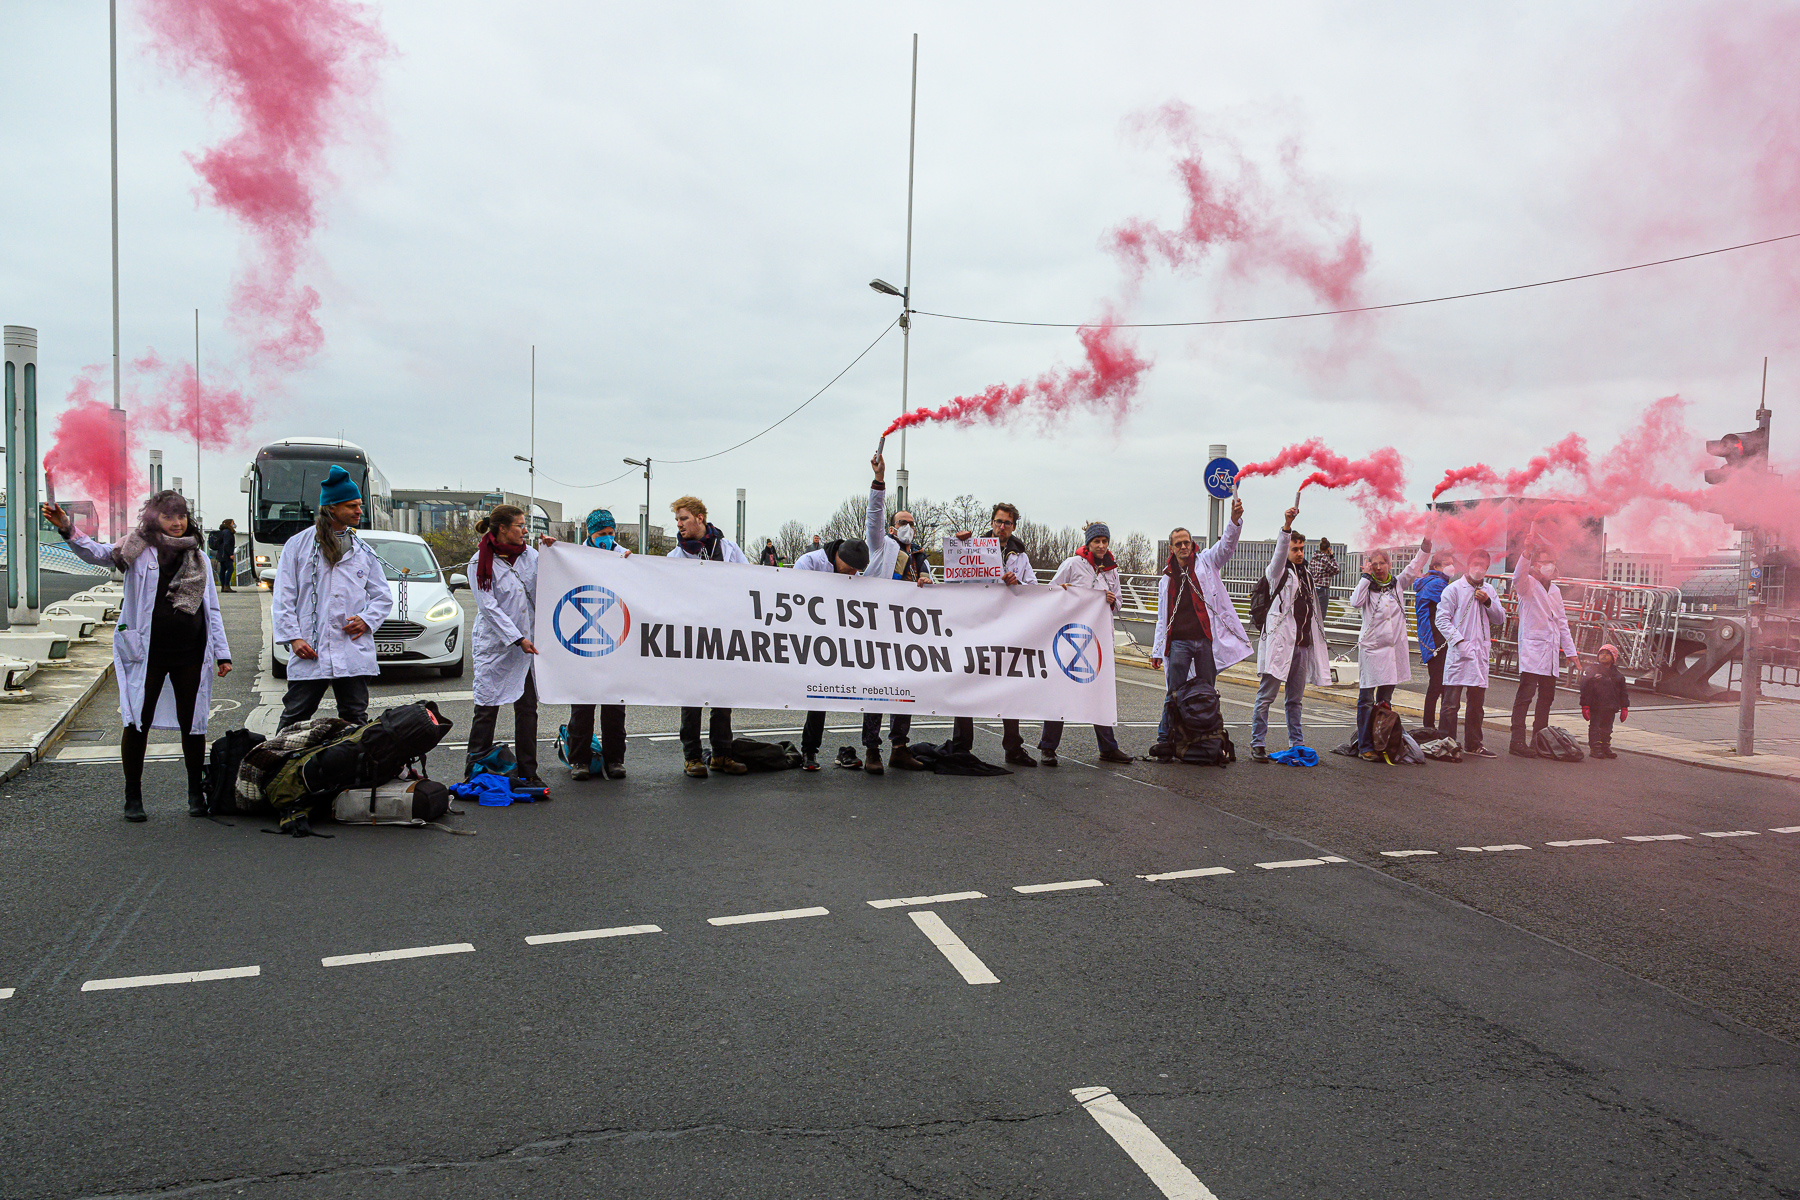
\includegraphics[width=\textwidth]{geteilte-Folien/Bilder/20220406-14-05-09.jpg}\\
\supertinycaption{% 
%Scientist Rebellion blockiert die Kronprinzenbrücke um auf Veröffentlichung IPCC-Report
%  hinzuweisen. 
Scientist Rebellion blockiert Kronprinzenbrücke in Berlin, 06.04.2022. Bild: CC-BY: Stefan Müller}
\end{column}
\begin{column}{35mm}
{\tiny
\begin{itemize}
\item[–] Andreas Zilker, Geograf,
\item[–] Anja Freiwald, Biotechnologin,
\item[–] Christian Bläul, Physiker
\item[–] Dr. Cornelia Huth, Ernährungswissenschaftlerin und Epidemologin, 
\item[–] Daniele Artico, Physiker,
%Florian Zander, 
\item[–] Friedrich Gräber, B.Sc. Biochemie,
%Harald Walsberg, Klimaaktion, Klimaschutz, 
\item[–] Kyle Topfer, Umweltwissenschaftler,
\item[–] Michael Hofmann, theoretischer Physiker,
\item[–] Dr. Nana-Maria Grüning, Biologin, 
\item[–] Prof. Dr. Nikolaus Froitzheim, Strukturgeograf,
\item[–] Dr. Stephanie Rach, Tierärztin,
\item[–] Wolfgang Metzeler-Kick, Ingenieur für technischen Umweltschutz,
\item[–] Dr. Valeria Scagliotti, Biologin,

\item[–] Seit 4/2022 internationale Proteste, auch Peter Kalmus, Klimaforscher bei NASA.

\#DontLookUp

\end{itemize}
}
\end{column}
\end{columns}

}

\frame{
\frametitlefit{Chomsky: I support the actions of the Just Stop Oil coalition}

\vfill\vfill
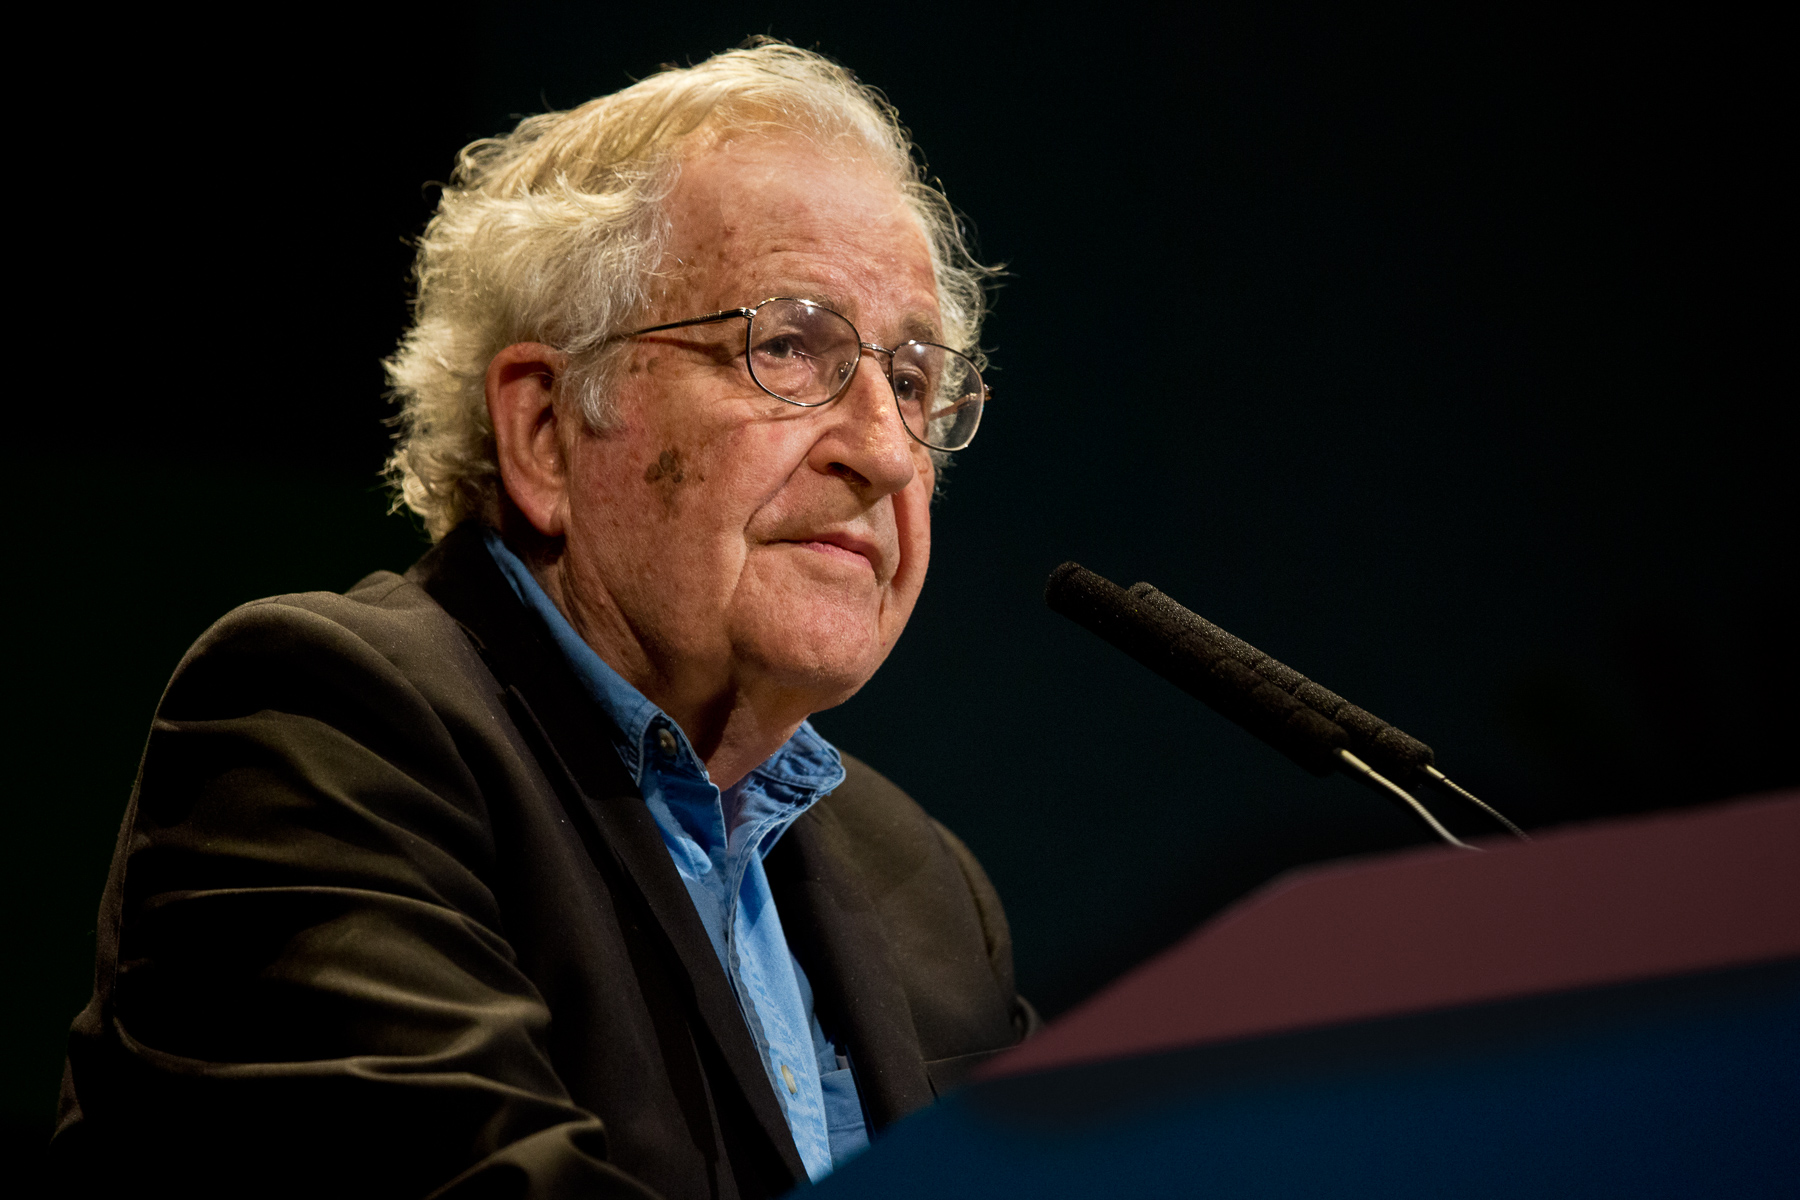
\includegraphics[width=0.65\textwidth]{geteilte-Folien/Bilder/chomsky-20150312-18-15-32.jpg}\\
\supertinycaption{% 
Noam Chomsky, 12.03.2015. Bild: CC-BY-SA: Augusto Starita}

\vfill

Video: \href{https://youtu.be/sTS04viZcGU}{Noam Chomsky on Just Stop Oil}

}

\frame{
\frametitle{Was ist Just Stop Oil? Was die Koalition?}

\begin{itemize}
\item Just Stop Oil ist eine britische Aktionsgruppe aus dem Extinction Rebellion-Umfeld.
\item Im Gegensatz zu XR blockieren sie keine Straßen, um die Politik zum Handeln aufzufordern,
sondern sie blockieren direkt relevante Infrastruktur.
\item Untertunnelung von Zufahrten zu Öl-Terminals.
\item Aus gewaltfreiem zivilem Ungehorsam ist gewaltfreier ziviler Widerstand geworden.

\bigskip

\item Was ist die Koalition?

\begin{itemize}
\item Scientist Rebellion (laut Prof. Niko Froitzheim, 13.05.2022, 1000 scientists weltweit)
\item Aufstand der Letzten Generation
\item Save old Growth (Kanada)
\item \ldots
\item Scientist Rebellion solidarisiert sich explizit mit dem Aufstand der Letzten Generation.
\end{itemize}
\end{itemize}


}

\frame[shrink=5]{
\frametitle{Katastrophenereignisse der letzten Jahre (2021--2022)}

\begin{itemize}
\item Kältewelle in den USA:
  \href{https://www.tagesschau.de/multimedia/video/video-827413.html}{Tagesschau 22.02.2021}

\item Hitze in USA/Kanada: \href{https://www.tagesschau.de/multimedia/video/video-884869.html}{Tagesschau 02.07.2021}

\item Starkregen in China (12 Tote):
  \href{https://www.tagesschau.de/multimedia/video/video-893071.html}{Tagesschau 21.07.2021} (U-Bahn)

\item Starkregen in New York (44 Tote):
  \href{https://www.tagesschau.de/multimedia/video/video-913415.html}{Tagesschau 03.09.2021}

%\item Welt: https://www.youtube.com/watch?v=msLx4ZdjUFU

\item Überflutungen Kanada (Notstand): \href{https://www.youtube.com/watch?v=3DKGoELrCN0}{Tageschau 18.11.2021}

\item Permafrostböden in der Arktis schmelzen:
  \href{https://www.mdr.de/wissen/arktis-fluesse-versiegen-rentier-eisbaer-dominoeffekt-100.html}{gute Doku im MDR}

\item Hochwasserkatastrophe in Henan, 300 Tote, 14 in U-Bahn, 200.000 evakuiert:
  \href{https://taz.de/Hochwasserkatastrophe-in-Henan/!5787142/}{taz 23.07.2021}, \href{https://www.tagesschau.de/ausland/asien/china-ueberschwemmungen-131.html}{Tagesschau 02.08.2021}



\item Antarktis 40° zu warm, Arktis 30°:
  \href{https://www.rnd.de/wissen/antarktis-temperaturen-40-grad-zu-hoch-ist-die-hitzewelle-nur-ein-aeusserst-unwahrscheinliches-3GKA6GBUIJBXHBS5OARICI2GNA.html}{rnd 22.03.2022}

\item Hunderte Millionen Menschen in Pakistan, Nord-Indien, Bangladesch  45°–48°
  \href{https://www.tagesschau.de/multimedia/video/video-1024679.html}{Tagesschau 29.04.2022},
  \href{https://www.bbc.com/news/world-asia-india-61242341}{BBC mit Film}
\end{itemize}

Is ja weit weg! Nee, isses nicht:  Ahrtal, Starkregen in Berlin 2017

30 Mrd € Schäden im Ahrtal 2021.\\
Auf Jahre Handwerker*innen beschäftigt.\\
Aber in diesem und jedem kommenden Jahr wird es neue Katastrophen geben.

Dürren. (\href{https://www.nationalgeographic.de/umwelt/2022/03/hydrologen-warnen-deutschland-trocknet-aus}{National
  Geographic, 22.03.2022})

Lieferketten gestört. 
%Teilweise durch Corona. Sich verstärkende Krisen. Und Zoonosen sind auch duch

}


\frame{
\frametitle{Folgen}

\begin{itemize}
\item Och, is doch schön, wenn's 'n bisschen wärmer wird.
\item Nee, isses nicht:\\
 Artensterben: Arten wanderen zu den Polen bzw. nach oben. 

Aber unterschiedliche Trigger:
  Temperatur bzw. Licht. 

Wenn Futter auf anderen Trigger reagiert, sterben Lebewesen aus. 

Die Ernährungskette wird löchrig. Es droht ein Kollaps. Wir sind mitten drin. (Hering in der Ostsee)

\item Regionen der Welt werden ubewohnbar. Hitze, Fluten.

\item Migration, Kriege.


\end{itemize}

}

\frame{
\frametitlefit{Prof. Dr. Maja Göpel zu existenziellen Bedrohungen der Menschheit}

\vfill
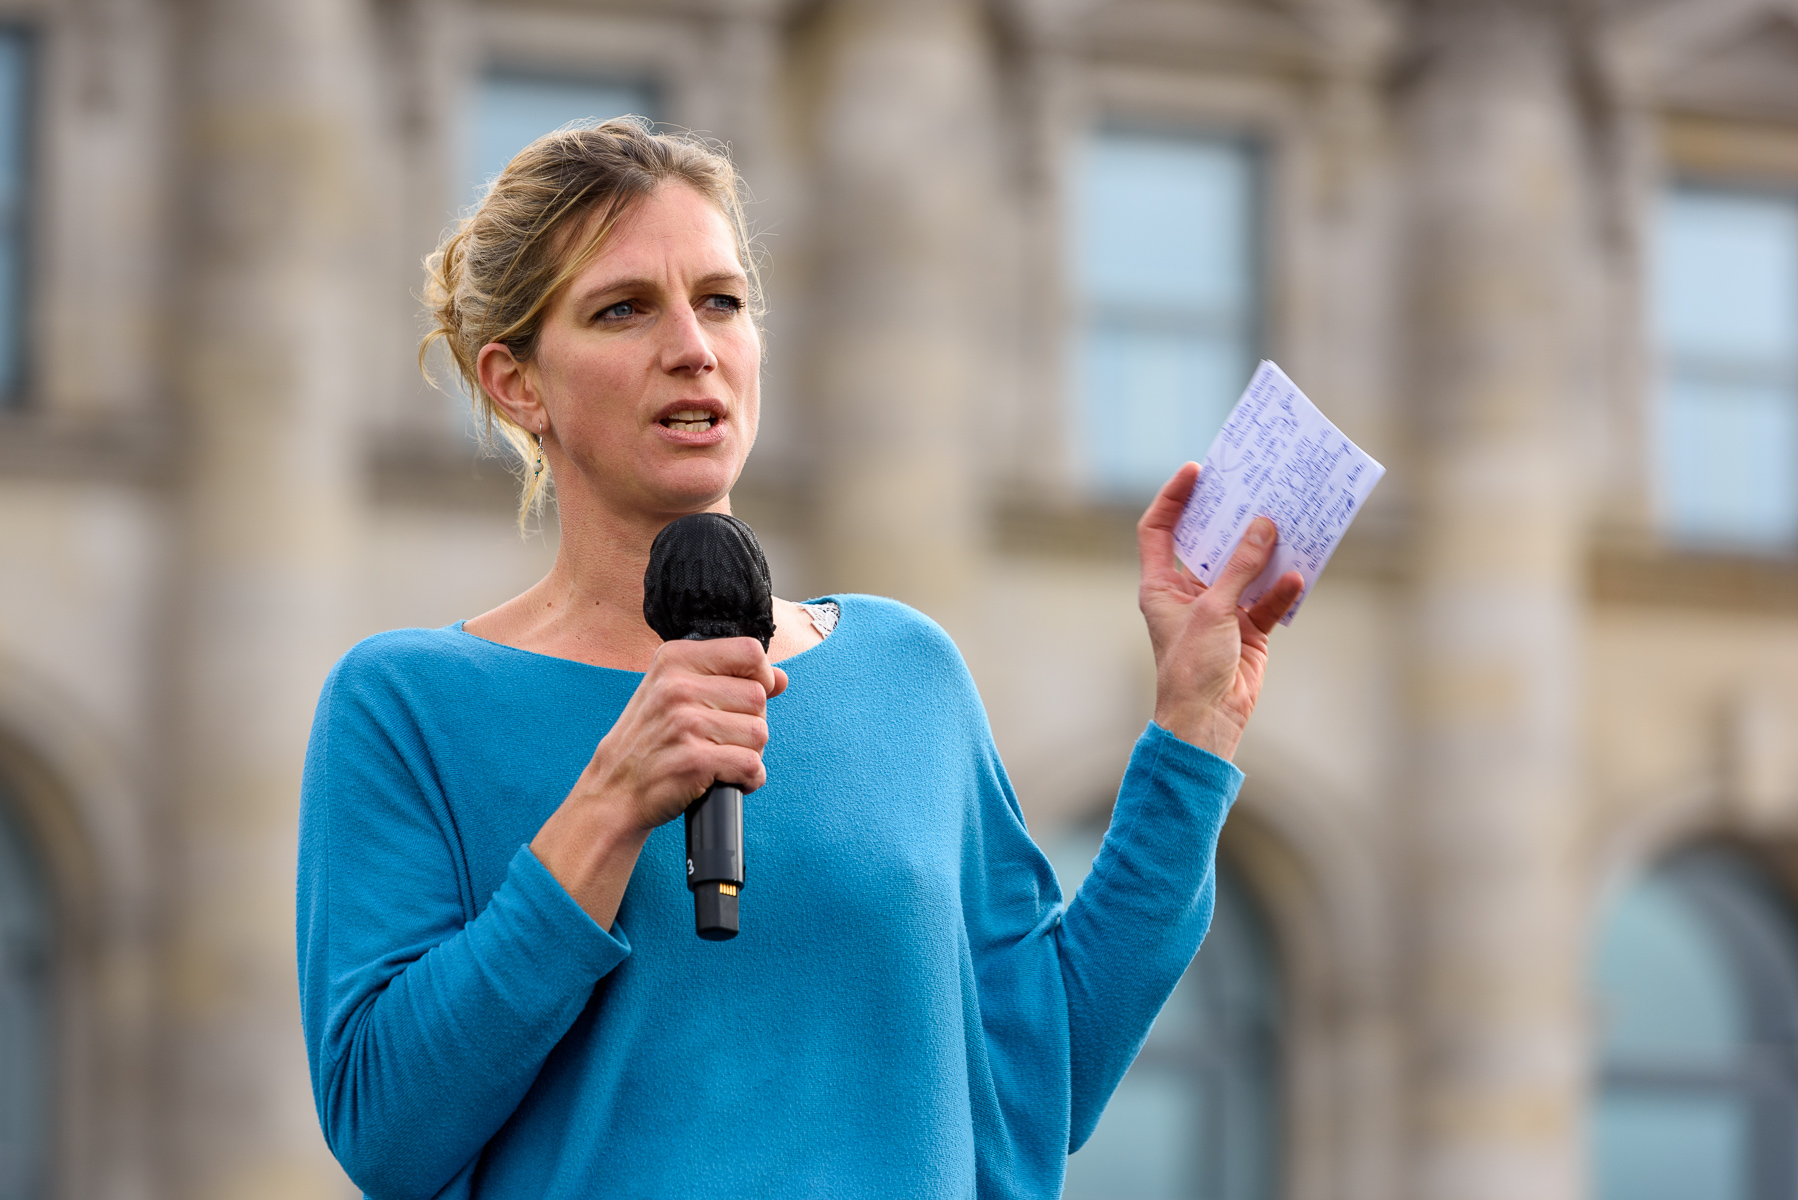
\includegraphics[width=0.65\textwidth]{geteilte-Folien/Bilder/20210924-12-39-42.jpg}\\
\supertinycaption{Maja Göpel spricht bei FFF am 24.09.2021, Bild CC-BY: Stefan Müller}
\vfill

\href{https://www.youtube.com/watch?v=Mp3z9z3Ecv4}{Video BPK}:
fünf ökologisch und die sechste Massenvernichtungswaffen
\vfill

}

\subsection{6.\ IPCC-Sachstandsbericht}

\frame{
\frametitle{Was ist los?}

\begin{itemize}
\item 6.\ IPCC-Sachstandsbericht
\item Die Lage ist verheerend. Das, was wir haben, haben wir bei 1,1° oder 1,2°. Angestrebt sind 1,5°
  also viel schlimmer. Aber so, wie wir jetzt handeln, kommen wir nicht bei 1,5° an.

\end{itemize}


}

\frame[shrink=5]{
\frametitle{CO2-Budget: Grad-Ziele, Budget und Wahrscheinlichkeiten}

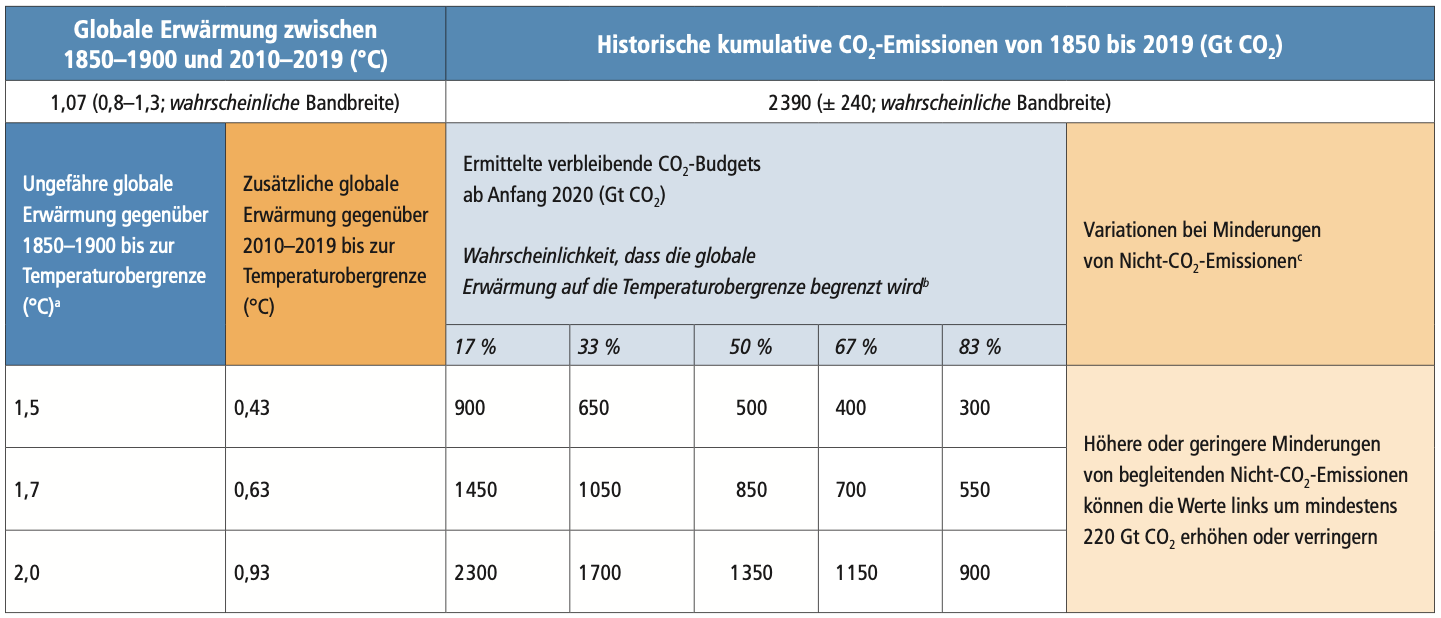
\includegraphics[width=\textwidth]{geteilte-Folien/Bilder/IPCC-CO2-Restbudget.png}\\

{\small
\begin{itemize}
\item 1,5° mit 83\,\% Wahrscheinlichkeit bedeutet ein Restbudget von 300Gt CO2.
\item Die Tabelle ist aber von Anfang 2020 \citep[\page 32]{IPCC2021-deutsch}.
\item Inzwischen haben wir weitere 70Gt CO2 emittiert.
\item Es bleiben also 230Gt für die ganze Welt.
\end{itemize}
}

}

\frame{
\frametitle{Der kleine Rest: CO2 historisch}

\begin{itemize}
\item Wie teilen wir den Rest auf? Gerecht natürlich! Aber was heißt das?
\item Es gibt fünf Verfahren für die Aufteilung \citep[\page 48]{Sachverstaendigenrat2020a}.
\item Wir setzen einfach die Zeit 1850 bis Ende CO2 an und geben allen Ländern gleiche
  Verschmutzungsrechte.
\item Upsi. Unsers ist ja schon alle. (Quelle: \href{https://www.carbonmap.org/\#Historical}{The Carbon Map})


\end{itemize}

\vfill
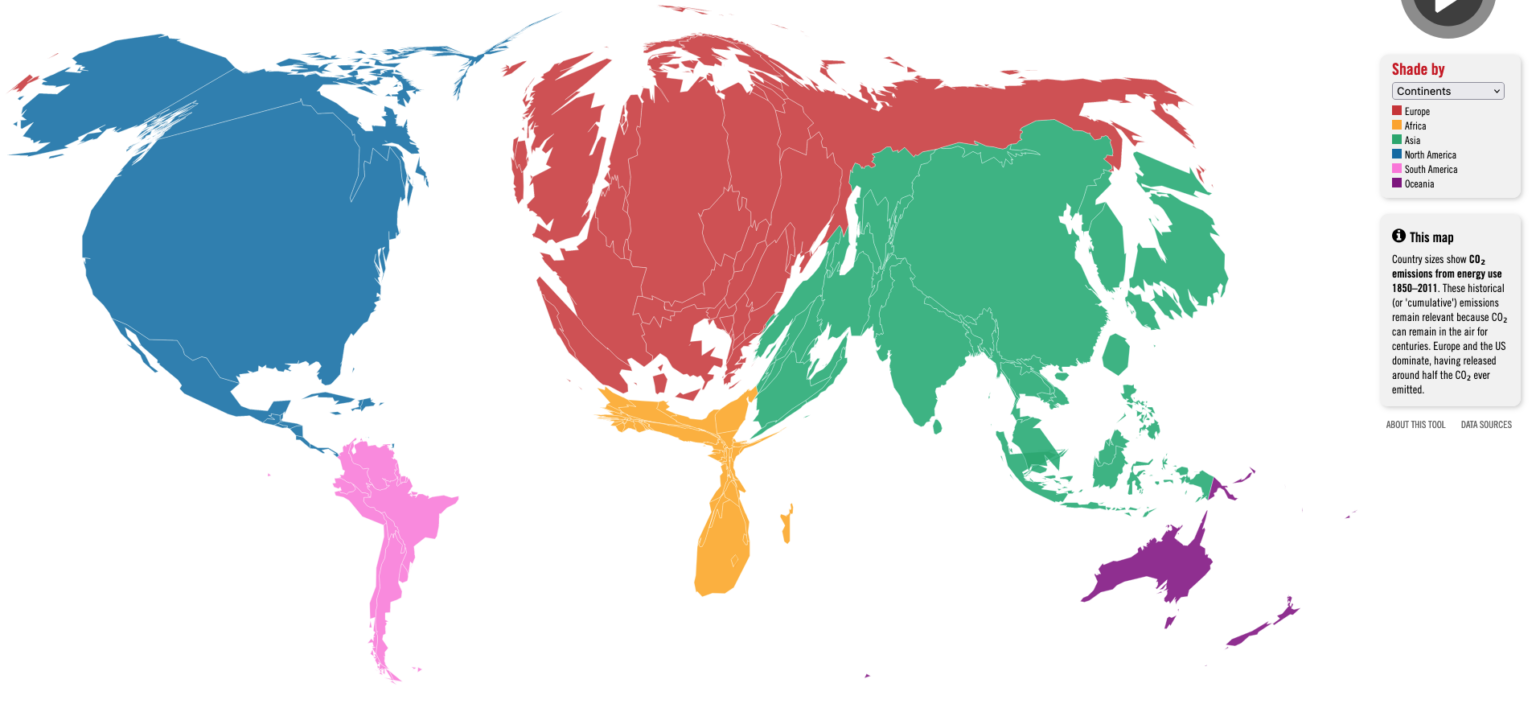
\includegraphics[width=.8\textwidth]{geteilte-Folien/Bilder/CO2-historisch.png}
\vfill

}

\frame{
\frametitle{CO2 pro lebendem Einwohner}

\begin{itemize}
\item Dann eben irgendwie anders gerecht. Wir teilen das unter den Lebenden auf.
\item D hat gegenwärtig 2\,\% des Ausstoßes, aber nur 1\,\% der Weltbevölkerung.
\item 1\,\% bedeutet 2,3 Gt für Deutschland.
\item "`Unter diesen ganzen Tonnen kann sich ja niemand etwas vorstellen."', Svenja Schulze,
  Bundesumweltministerin 2019 auf die Frage, wie hoch denn unser Restbudget wäre.
\item Was bedeutet das für jede/n Einzelnen. 2,3Gt / 83 Mio = 27,7 t.
\item Der Durchschnitts CO2-Ausstoß pro Person in Deutschland sind 9–11t pro Jahr.
\item Das heißt: In drei Jahren ist alles alle.
\end{itemize}

}

\frame{
\frametitle{Wir machen es anteilig, wie immer}

\begin{itemize}
\item Gerecht per Kopf geht ja nicht! Wir können ja nicht plötzlich, \ldots (Sarcasm)
\item Methode: grandfathering:\\
      Wir machen weiter Dreck, weil wir das schon immer gemacht haben.
\item Westen darf mehr als Entwicklungsländer. Das ist die Methode der EU.
\item Die gute Nachricht: Wir haben dann noch doppelt so lange Zeit.
\item Upsi. Sind ja auch nur sechs Jahre.

%\item Sechs Jahre = 1 freiwilliges soziales Jahr + Studium.

\bigskip

\item Nebenbemerkung: Wenn jeder sich seine Lieblingsmethode aussucht, landen wir bei
  3,2°. \citep[\page 48]{Sachverstaendigenrat2020a}


\end{itemize}


}

\frame{
\frametitle{Zur Einordnung: ein einzelnes Auto $\to$ alles weg}

\begin{itemize}
\item Autos sind in Deutschland durchschnittlich 10 Jahre zugelassen.
\item In dieser Zeit stoßen Verbrenner so viel CO2 aus, wie jeder noch übrig hat.
\item Dabei ist die Herstellung nicht berücksichtigt. Ja nach Auto 10–30t.
\item Die Herstellung fällt auch bei E-Autos an.
\item $\to$ Car is over.
\end{itemize}

\flushright\vspace{-7mm}\begin{tabular}{@{}l@{}}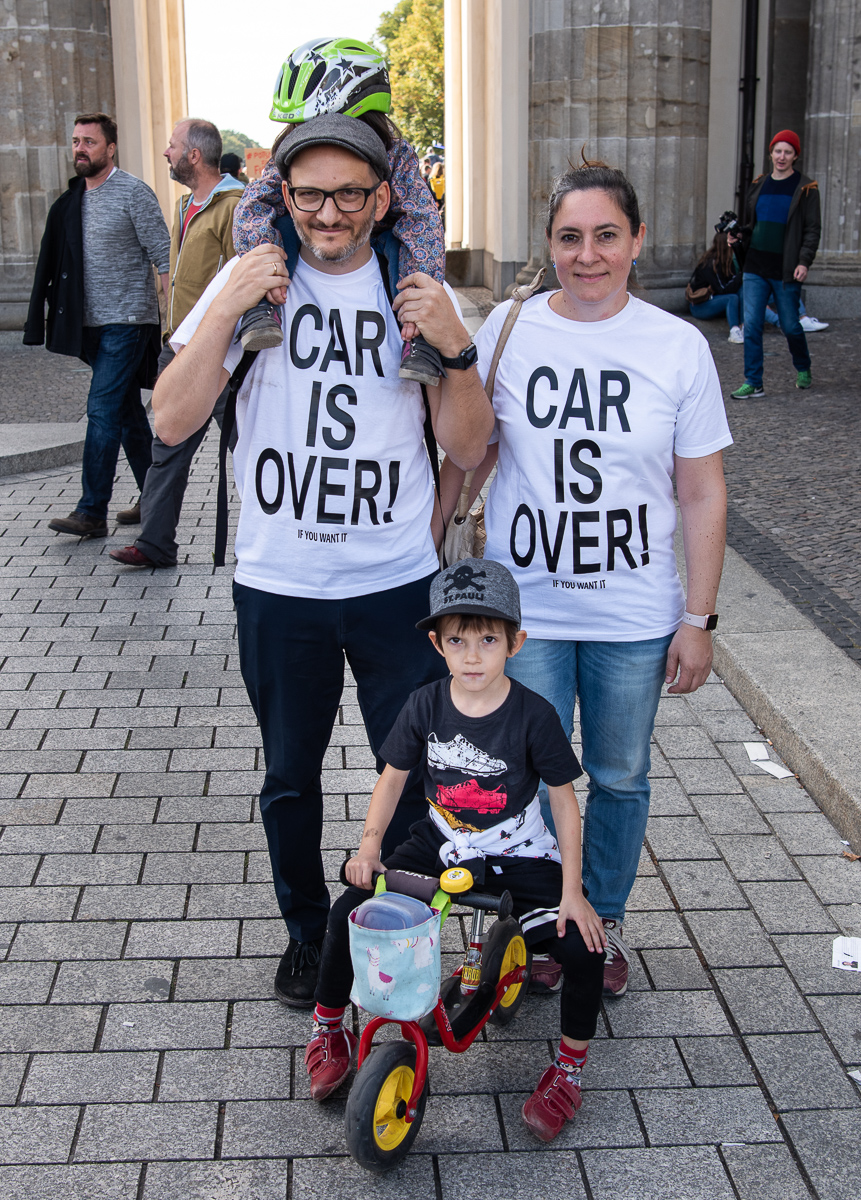
\includegraphics[width=.27\textwidth]{geteilte-Folien/Bilder/car-is-over-20190920-15-06-18.jpg}\\
\raisebox{2mm}[0pt][0pt]{\supertinycaption{Bei FFF, 20.09.2019, CC-BY St Mü}}\end{tabular}\hspace{8mm}


}


\subsection{UN-Generalsekretär António Guterres}

\frame{
\frametitle{UN-Generalsekretär António Guterres}


\begin{itemize}
\item António Guterres: \href{https://media.un.org/en/asset/k1x/k1xcijxjhp}{Link}

\item Amtliche Übersetzung auf Deutsch: \href{https://unric.org/de/ipcc280202022/}{Link}



\end{itemize}


}


\frame[shrink=5]{
\frametitlefit{Blockierer*innen hätten sich den Text nicht passender ausdenken können}

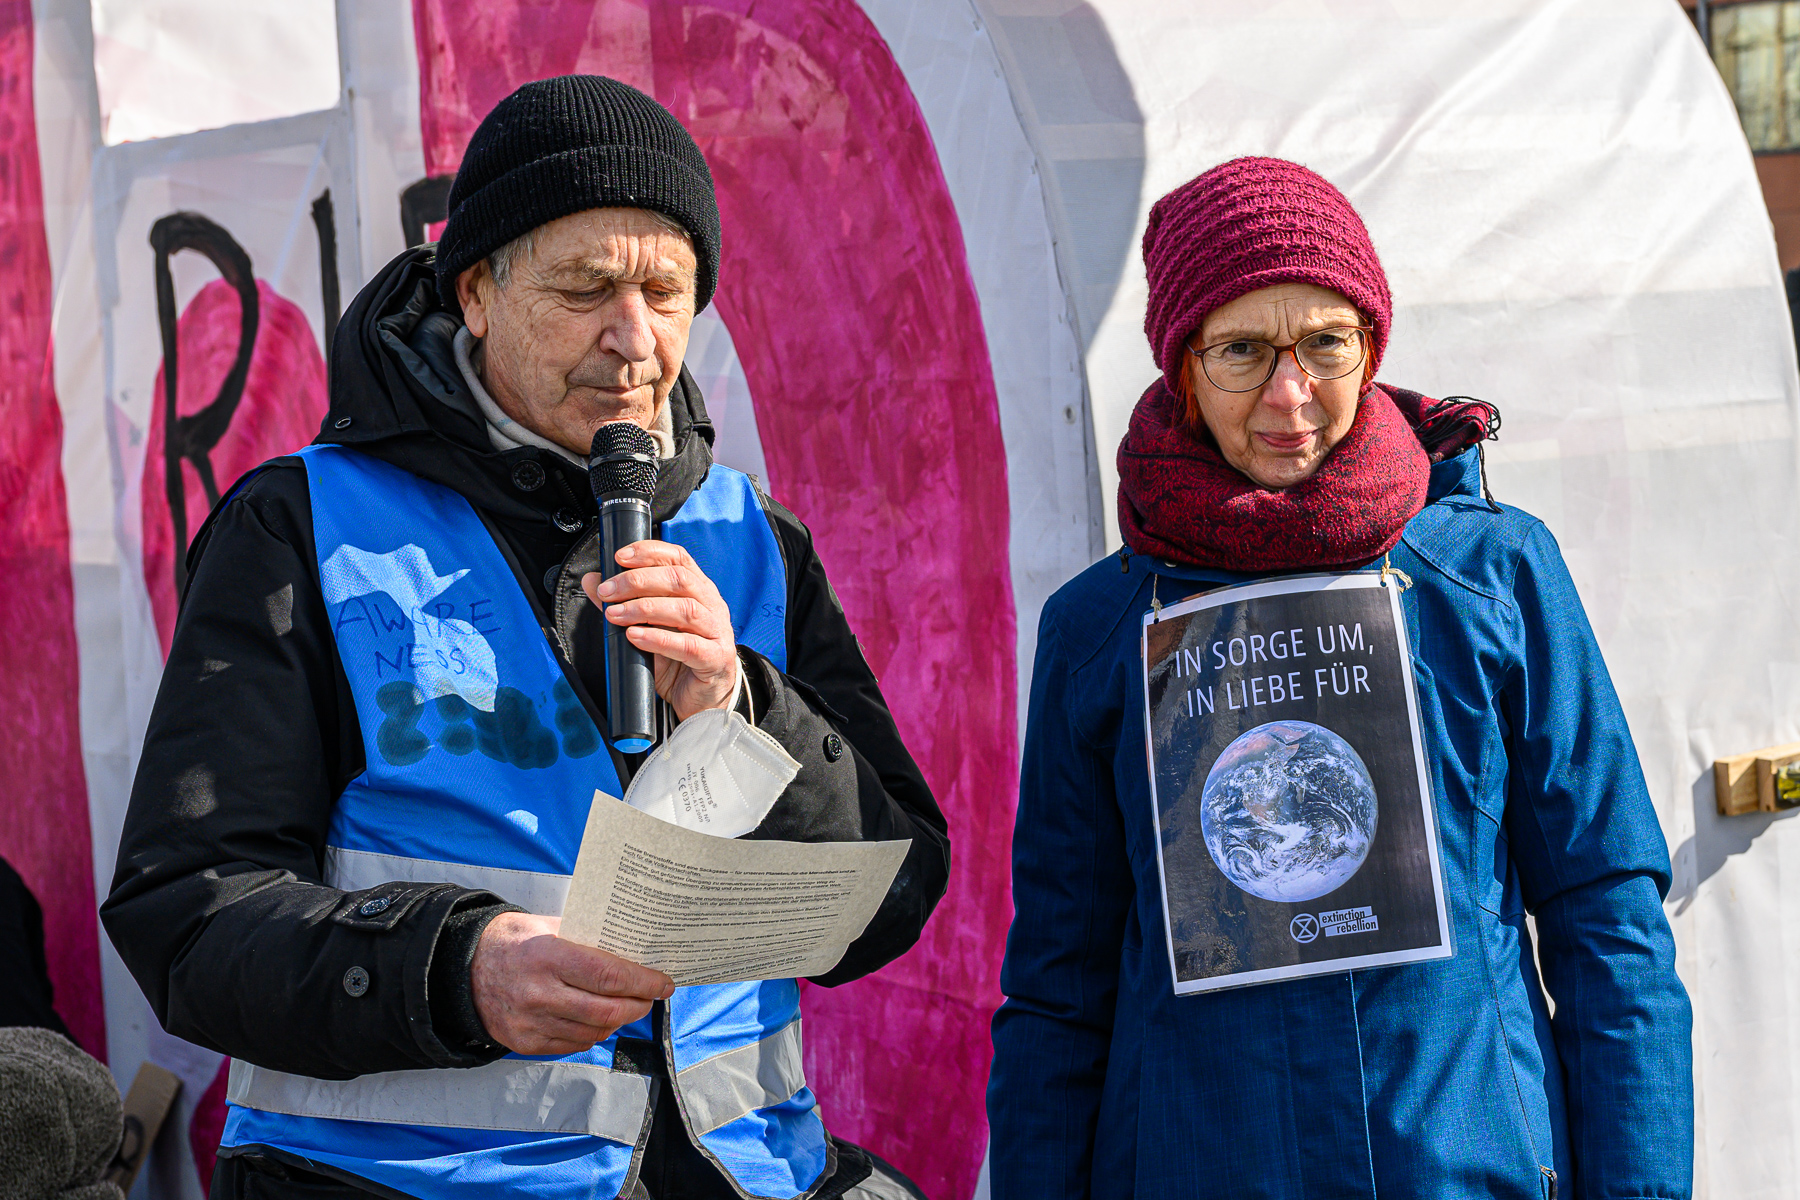
\includegraphics[width=.5\textwidth]{geteilte-Folien/Bilder/20220305-13-26-59.jpg}\\
\supertinycaption{Blockade der Marschallbrücke in Berlin durch Extinction Rebellion, 05.03.22. Bild: CC-BY Stefan Müller}

\tiny
„Die G20 müssen mit gutem Beispiel vorangehen, sonst wird die Menschheit einen noch tragischeren Preis zahlen.

Ich weiß, dass die Menschen überall ängstlich und wütend sind.

Ich bin es auch.

Jetzt ist es an der Zeit, die Wut in Taten umzusetzen.

Jeder Bruchteil eines Grades zählt.

Jede Stimme kann einen Unterschied machen.

Und jede Sekunde zählt.

Ich danke Ihnen.“ António Guterres, 28.02.2022


}




\frame[shrink=5]{
\frametitle{Was kann man selbst tun?}


Es ist schlimm, wenn man das Gefühl hat, selbst nichts tun zu können.\\
Ein bisschen kann man tun:
\begin{itemize}
\item weniger/kein Fleisch essen
\item weniger/nicht fliegen
\item In der Stadt Auto abschaffen. Sonst weniger/anders fahren.
\item weniger/anders heizen und lüften
\end{itemize}

\pause
Wichtiger sind aber die großen gesellschaftlichen Veränderungen.
\begin{itemize}
\item politisch aktiv werden/bleiben
\item Bürger*innenrat (Vertreter*innen alle Parteien wollen das inzwischen: Koalition, Schäubele,
  Köhler, \ldots)
\begin{itemize}
\item Steuern
\item Tempolimit
\item Agrarwende, Verkehrswende, Energiewende
\item usw.
\end{itemize}
\item Für all das gibt es Mehrheiten in der Bevölkerung.\\
      Klimaräte in Frankreich und Dänemark waren erfolgreich.\\
      Es gab auch in D schon einen (\href{taz, 25.06.2021}{taz, 25.06.2021})
\end{itemize}


}


\frame{
\frametitle{Was müssen wir alle gemeinsam tun?}


\begin{itemize}
\item Just stop oil! (und Kohle) "`It's now or never! Failure is not an option!"' (Chomsky, 2022)
\item Guardian: Carbon Bombs \href{https://www.theguardian.com/environment/ng-interactive/2022/may/11/fossil-fuel-carbon-bombs-climate-breakdown-oil-gas}{Link}
\item Lea Dohm (Psychologists for Future, 13.05.2022):\\ Macht, was Ihr am besten könnt,\\ was Euch Spaß
  macht.\\Macht es in der Gruppe.

\end{itemize}

}

\frame{
\frametitle{Zum Beispiel: Stadtradeln}

\begin{itemize}
\item Habe ich gerade zum Aufstand aufgerufen?
\item Ach i wo.
\item Wir machen alle Stadtradeln. In der Gruppe!
\item Das unschlagbare Linguisten-Team hat schon 27 Mitglieder.
\item Link ist im Moodle.
\end{itemize}

}
% %\include{hpsg-komplexe-praedikate}

\appendix
% muss immer geladen werden, wegen Referenzen
%\section<presentation>*{Literatur}

%% \frame{
%%   \frametitle<presentation>{Literatur}
  
%%   \beamertemplatebookbibitems

%% \bibliography{biblio}
%% \bibliographystyle{natbib.myfullname}
%% }
%\beamertemplatebookbibitems

% there seems to be a bug. These things are only set on the first literature slide
%
% The bug is still there, but the fix does not work any longer. 
\iflanguage{german}{\renewcommand{\refname}{Literaturverzeichnis}} % should be set automatically ???
%\iflanguage{german}{\def\insertsectionhead{Literaturverzeichnis}}{\def\insertsectionhead{\refname}}
\def\insertsectionhead{\refname}
\def\insertsubsectionhead{}

\huberlinjustbarfootline

\ifpdf
\else
\ifxetex
\else
\let\url=\burl
\fi
\fi
\begin{multicols}{2}
{\renewcommand*{\bibfont}{\tiny}

%\beamertemplatearticlebibitems

%\bibliography{bib-abbr,biblio,crossrefs}
%\bibliographystyle{unified}

% biblatex

%\addbibresource{bib-abbr.bib,biblio.bib}

% no book icon please
\setbeamertemplate{bibliography item}{}

%\printbibliography
\printbibliography[heading=bibliography,notkeyword=this] 

}
\end{multicols}




\end{document}


% Local variables:
% mode: lazy-lock
% End:


















